\documentclass[twoside]{book}

% Packages required by doxygen
\usepackage{fixltx2e}
\usepackage{calc}
\usepackage{doxygen}
\usepackage[export]{adjustbox} % also loads graphicx
\usepackage{graphicx}
\usepackage[utf8]{inputenc}
\usepackage{makeidx}
\usepackage{multicol}
\usepackage{multirow}
\PassOptionsToPackage{warn}{textcomp}
\usepackage{textcomp}
\usepackage[nointegrals]{wasysym}
\usepackage[table]{xcolor}

% Font selection
\usepackage[T1]{fontenc}
\usepackage[scaled=.90]{helvet}
\usepackage{courier}
\usepackage{amssymb}
\usepackage{sectsty}
\renewcommand{\familydefault}{\sfdefault}
\allsectionsfont{%
  \fontseries{bc}\selectfont%
  \color{darkgray}%
}
\renewcommand{\DoxyLabelFont}{%
  \fontseries{bc}\selectfont%
  \color{darkgray}%
}
\newcommand{\+}{\discretionary{\mbox{\scriptsize$\hookleftarrow$}}{}{}}

% Page & text layout
\usepackage{geometry}
\geometry{%
  a4paper,%
  top=2.5cm,%
  bottom=2.5cm,%
  left=2.5cm,%
  right=2.5cm%
}
\tolerance=750
\hfuzz=15pt
\hbadness=750
\setlength{\emergencystretch}{15pt}
\setlength{\parindent}{0cm}
\setlength{\parskip}{3ex plus 2ex minus 2ex}
\makeatletter
\renewcommand{\paragraph}{%
  \@startsection{paragraph}{4}{0ex}{-1.0ex}{1.0ex}{%
    \normalfont\normalsize\bfseries\SS@parafont%
  }%
}
\renewcommand{\subparagraph}{%
  \@startsection{subparagraph}{5}{0ex}{-1.0ex}{1.0ex}{%
    \normalfont\normalsize\bfseries\SS@subparafont%
  }%
}
\makeatother

% Headers & footers
\usepackage{fancyhdr}
\pagestyle{fancyplain}
\fancyhead[LE]{\fancyplain{}{\bfseries\thepage}}
\fancyhead[CE]{\fancyplain{}{}}
\fancyhead[RE]{\fancyplain{}{\bfseries\leftmark}}
\fancyhead[LO]{\fancyplain{}{\bfseries\rightmark}}
\fancyhead[CO]{\fancyplain{}{}}
\fancyhead[RO]{\fancyplain{}{\bfseries\thepage}}
\fancyfoot[LE]{\fancyplain{}{}}
\fancyfoot[CE]{\fancyplain{}{}}
\fancyfoot[RE]{\fancyplain{}{\bfseries\scriptsize Generated by Doxygen }}
\fancyfoot[LO]{\fancyplain{}{\bfseries\scriptsize Generated by Doxygen }}
\fancyfoot[CO]{\fancyplain{}{}}
\fancyfoot[RO]{\fancyplain{}{}}
\renewcommand{\footrulewidth}{0.4pt}
\renewcommand{\chaptermark}[1]{%
  \markboth{#1}{}%
}
\renewcommand{\sectionmark}[1]{%
  \markright{\thesection\ #1}%
}

% Indices & bibliography
\usepackage{natbib}
\usepackage[titles]{tocloft}
\setcounter{tocdepth}{3}
\setcounter{secnumdepth}{5}
\makeindex

% Hyperlinks (required, but should be loaded last)
\usepackage{ifpdf}
\ifpdf
  \usepackage[pdftex,pagebackref=true]{hyperref}
\else
  \usepackage[ps2pdf,pagebackref=true]{hyperref}
\fi
\hypersetup{%
  colorlinks=true,%
  linkcolor=blue,%
  citecolor=blue,%
  unicode%
}

% Custom commands
\newcommand{\clearemptydoublepage}{%
  \newpage{\pagestyle{empty}\cleardoublepage}%
}

\usepackage{caption}
\captionsetup{labelsep=space,justification=centering,font={bf},singlelinecheck=off,skip=4pt,position=top}

%===== C O N T E N T S =====

\begin{document}

% Titlepage & ToC
\hypersetup{pageanchor=false,
             bookmarksnumbered=true,
             pdfencoding=unicode
            }
\pagenumbering{alph}
\begin{titlepage}
\vspace*{7cm}
\begin{center}%
{\Large My Project }\\
\vspace*{1cm}
{\large Generated by Doxygen 1.8.14}\\
\end{center}
\end{titlepage}
\clearemptydoublepage
\pagenumbering{roman}
\tableofcontents
\clearemptydoublepage
\pagenumbering{arabic}
\hypersetup{pageanchor=true}

%--- Begin generated contents ---
\chapter{Hierarchical Index}
\section{Class Hierarchy}
This inheritance list is sorted roughly, but not completely, alphabetically\+:\begin{DoxyCompactList}
\item \contentsline{section}{boost\+:\+:winapi\+:\+:\+\_\+\+L\+U\+I\+D\+\_\+}{\pageref{structboost_1_1winapi_1_1___l_u_i_d__}}{}
\item \contentsline{section}{boost\+:\+:winapi\+:\+:\+\_\+\+L\+U\+I\+D\+\_\+\+A\+N\+D\+\_\+\+A\+T\+T\+R\+I\+B\+U\+T\+E\+S\+\_\+}{\pageref{structboost_1_1winapi_1_1___l_u_i_d___a_n_d___a_t_t_r_i_b_u_t_e_s__}}{}
\item \contentsline{section}{boost\+:\+:winapi\+:\+:\+\_\+\+P\+R\+I\+V\+I\+L\+E\+G\+E\+\_\+\+S\+E\+T\+\_\+}{\pageref{structboost_1_1winapi_1_1___p_r_i_v_i_l_e_g_e___s_e_t__}}{}
\item \contentsline{section}{boost\+:\+:winapi\+:\+:\+\_\+\+P\+R\+O\+C\+E\+S\+S\+\_\+\+M\+E\+M\+O\+R\+Y\+\_\+\+C\+O\+U\+N\+T\+E\+R\+S\+\_\+}{\pageref{structboost_1_1winapi_1_1___p_r_o_c_e_s_s___m_e_m_o_r_y___c_o_u_n_t_e_r_s__}}{}
\item \contentsline{section}{boost\+:\+:winapi\+:\+:\+\_\+\+P\+R\+O\+C\+E\+S\+S\+\_\+\+M\+E\+M\+O\+R\+Y\+\_\+\+C\+O\+U\+N\+T\+E\+R\+S\+\_\+\+E\+X\+\_\+}{\pageref{structboost_1_1winapi_1_1___p_r_o_c_e_s_s___m_e_m_o_r_y___c_o_u_n_t_e_r_s___e_x__}}{}
\item \contentsline{section}{boost\+:\+:winapi\+:\+:\+\_\+\+T\+O\+K\+E\+N\+\_\+\+P\+R\+I\+V\+I\+L\+E\+G\+E\+S\+\_\+}{\pageref{structboost_1_1winapi_1_1___t_o_k_e_n___p_r_i_v_i_l_e_g_e_s__}}{}
\item \contentsline{section}{distant\+:\+:access\+\_\+rights}{\pageref{structdistant_1_1access__rights}}{}
\item \contentsline{section}{distant\+:\+:memory\+:\+:address$<$ AddressT $>$}{\pageref{classdistant_1_1memory_1_1address}}{}
\item \contentsline{section}{address\+\_\+space}{\pageref{classaddress__space}}{}
\item \contentsline{section}{distant\+:\+:function\+\_\+traits$<$ function$<$ R(Args...), Calling\+Conv, AddressT $>$ $>$\+:\+:argument$<$ N $>$}{\pageref{structdistant_1_1function__traits_3_01function_3_01_r_07_args_8_8_8_08_00_01_calling_conv_00_01_address_t_01_4_01_4_1_1argument}}{}
\item \contentsline{section}{distant\+:\+:utility\+:\+:boolean\+\_\+validator$<$ Derived $>$}{\pageref{classdistant_1_1utility_1_1boolean__validator}}{}
\item \contentsline{section}{distant\+:\+:utility\+:\+:boolean\+\_\+validator$<$ handle\+\_\+base $>$}{\pageref{classdistant_1_1utility_1_1boolean__validator}}{}
\begin{DoxyCompactList}
\item \contentsline{section}{distant\+:\+:detail\+:\+:handle\+\_\+base}{\pageref{classdistant_1_1detail_1_1handle__base}}{}
\begin{DoxyCompactList}
\item \contentsline{section}{distant\+:\+:handle$<$ ObjectT $>$}{\pageref{classdistant_1_1handle}}{}
\item \contentsline{section}{distant\+:\+:handle$<$ distant\+:\+:kernel\+\_\+objects\+:\+:process\+\_\+base $>$}{\pageref{classdistant_1_1handle}}{}
\item \contentsline{section}{distant\+:\+:handle$<$ distant\+:\+:kernel\+\_\+objects\+:\+:snapshot $>$}{\pageref{classdistant_1_1handle}}{}
\item \contentsline{section}{distant\+:\+:handle$<$ distant\+:\+:kernel\+\_\+objects\+:\+:thread $>$}{\pageref{classdistant_1_1handle}}{}
\item \contentsline{section}{distant\+:\+:handle$<$ distant\+:\+:synch\+:\+:mutex $>$}{\pageref{classdistant_1_1handle}}{}
\item \contentsline{section}{distant\+:\+:handle$<$ kernel\+\_\+object $>$}{\pageref{classdistant_1_1handle}}{}
\end{DoxyCompactList}
\end{DoxyCompactList}
\item \contentsline{section}{distant\+:\+:utility\+:\+:boolean\+\_\+validator$<$ kernel\+\_\+object $>$}{\pageref{classdistant_1_1utility_1_1boolean__validator}}{}
\begin{DoxyCompactList}
\item \contentsline{section}{distant\+:\+:kernel\+\_\+objects\+:\+:kernel\+\_\+object}{\pageref{classdistant_1_1kernel__objects_1_1kernel__object}}{}
\begin{DoxyCompactList}
\item \contentsline{section}{distant\+:\+:kernel\+\_\+objects\+:\+:access\+\_\+token$<$ Access, Kernel\+Object $>$}{\pageref{classdistant_1_1kernel__objects_1_1access__token}}{}
\item \contentsline{section}{distant\+:\+:kernel\+\_\+objects\+:\+:securable}{\pageref{classdistant_1_1kernel__objects_1_1securable}}{}
\end{DoxyCompactList}
\end{DoxyCompactList}
\item \contentsline{section}{distant\+:\+:utility\+:\+:boolean\+\_\+validator$<$ snapshot$<$ Kernel\+Object $>$ $>$}{\pageref{classdistant_1_1utility_1_1boolean__validator}}{}
\begin{DoxyCompactList}
\item \contentsline{section}{distant\+:\+:kernel\+\_\+objects\+:\+:snapshot$<$ Kernel\+Object $>$}{\pageref{classdistant_1_1kernel__objects_1_1snapshot}}{}
\end{DoxyCompactList}
\item \contentsline{section}{distant\+:\+:memory\+:\+:x86\+\_\+calling\+\_\+conventions\+:\+:cdeclcall}{\pageref{structdistant_1_1memory_1_1x86__calling__conventions_1_1cdeclcall}}{}
\item \contentsline{section}{distant\+:\+:utility\+:\+:detail\+:\+:detector$<$ Default, Always\+Void, Op, Args $>$}{\pageref{structdistant_1_1utility_1_1detail_1_1detector}}{}
\item \contentsline{section}{distant\+:\+:utility\+:\+:detail\+:\+:detector$<$ Default, std\+:\+:void\+\_\+t$<$ Op$<$ Args... $>$ $>$, Op, Args... $>$}{\pageref{structdistant_1_1utility_1_1detail_1_1detector_3_01_default_00_01std_1_1void__t_3_01_op_3_01_arg04e1ee669e2093134af6db72a2dfc0d6}}{}
\item \contentsline{section}{distant\+:\+:kernel\+\_\+objects\+:\+:detail\+:\+:dispatcher$<$ Object $>$}{\pageref{structdistant_1_1kernel__objects_1_1detail_1_1dispatcher}}{}
\item \contentsline{section}{distant\+:\+:kernel\+\_\+objects\+:\+:detail\+:\+:dispatcher$<$ process$<$ A $>$ $>$}{\pageref{structdistant_1_1kernel__objects_1_1detail_1_1dispatcher_3_01process_3_01_a_01_4_01_4}}{}
\item \contentsline{section}{distant\+:\+:kernel\+\_\+objects\+:\+:detail\+:\+:dispatcher$<$ process\+\_\+base $>$}{\pageref{structdistant_1_1kernel__objects_1_1detail_1_1dispatcher_3_01process__base_01_4}}{}
\item \contentsline{section}{distant\+:\+:assembly\+:\+:dword\+\_\+ptr\+\_\+t$<$ T, typename $>$}{\pageref{structdistant_1_1assembly_1_1dword__ptr__t}}{}
\item error\+\_\+category\begin{DoxyCompactList}
\item \contentsline{section}{distant\+:\+:error\+:\+:windows\+\_\+category}{\pageref{classdistant_1_1error_1_1windows__category}}{}
\end{DoxyCompactList}
\item error\+\_\+code\begin{DoxyCompactList}
\item \contentsline{section}{distant\+:\+:error\+:\+:windows\+\_\+error\+\_\+code}{\pageref{classdistant_1_1error_1_1windows__error__code}}{}
\end{DoxyCompactList}
\item \contentsline{section}{distant\+:\+:memory\+:\+:x86\+\_\+calling\+\_\+conventions\+:\+:fastcall}{\pageref{structdistant_1_1memory_1_1x86__calling__conventions_1_1fastcall}}{}
\item \contentsline{section}{distant\+:\+:memory\+:\+:function$<$ Signature, Calling\+Conv, AddressT $>$}{\pageref{classdistant_1_1memory_1_1function}}{}
\item \contentsline{section}{distant\+:\+:memory\+:\+:function$<$ R(Args...), Calling\+Conv, AddressT $>$}{\pageref{classdistant_1_1memory_1_1function_3_01_r_07_args_8_8_8_08_00_01_calling_conv_00_01_address_t_01_4}}{}
\item \contentsline{section}{distant\+:\+:function\+\_\+traits$<$ F $>$}{\pageref{structdistant_1_1function__traits}}{}
\item \contentsline{section}{distant\+:\+:function\+\_\+traits$<$ function$<$ R(Args...), Calling\+Conv, AddressT $>$ $>$}{\pageref{structdistant_1_1function__traits_3_01function_3_01_r_07_args_8_8_8_08_00_01_calling_conv_00_01_address_t_01_4_01_4}}{}
\item \contentsline{section}{distant\+:\+:get\+\_\+access\+\_\+rights$<$ Object $>$}{\pageref{structdistant_1_1get__access__rights}}{}
\item \contentsline{section}{distant\+:\+:get\+\_\+access\+\_\+rights$<$ kernel\+\_\+objects\+:\+:process$<$ Access $>$ $>$}{\pageref{structdistant_1_1get__access__rights_3_01kernel__objects_1_1process_3_01_access_01_4_01_4}}{}
\item \contentsline{section}{distant\+:\+:error\+:\+:gle}{\pageref{structdistant_1_1error_1_1gle}}{}
\item \contentsline{section}{distant\+:\+:kernel\+\_\+objects\+:\+:detail\+:\+:has\+\_\+token\+\_\+access$<$ typename $>$}{\pageref{structdistant_1_1kernel__objects_1_1detail_1_1has__token__access}}{}
\item \contentsline{section}{distant\+:\+:kernel\+\_\+objects\+:\+:detail\+:\+:has\+\_\+token\+\_\+access$<$ process$<$ A $>$ $>$}{\pageref{structdistant_1_1kernel__objects_1_1detail_1_1has__token__access_3_01process_3_01_a_01_4_01_4}}{}
\item \contentsline{section}{distant\+:\+:utility\+:\+:meta\+:\+:hash$<$ T $>$}{\pageref{structdistant_1_1utility_1_1meta_1_1hash}}{}
\item \contentsline{section}{std\+:\+:hash$<$ distant\+:\+:memory\+:\+:address$<$ A $>$ $>$}{\pageref{structstd_1_1hash_3_01distant_1_1memory_1_1address_3_01_a_01_4_01_4}}{}
\item \contentsline{section}{distant\+:\+:is\+\_\+kernel\+\_\+object$<$ T $>$}{\pageref{structdistant_1_1is__kernel__object}}{}
\item iterator\+\_\+facade\begin{DoxyCompactList}
\item \contentsline{section}{distant\+:\+:assembly\+:\+:static\+\_\+assembler\+\_\+iterator$<$ Assembler\+Size, Instr\+Count $>$}{\pageref{classdistant_1_1assembly_1_1static__assembler__iterator}}{}
\item \contentsline{section}{distant\+:\+:kernel\+\_\+objects\+:\+:snapshot\+\_\+iterator$<$ Kernel\+Object $>$}{\pageref{classdistant_1_1kernel__objects_1_1snapshot__iterator}}{}
\item \contentsline{section}{distant\+:\+:memory\+:\+:virtual\+\_\+ptr$<$ Element, AddressT $>$}{\pageref{classdistant_1_1memory_1_1virtual__ptr}}{}
\item \contentsline{section}{distant\+:\+:memory\+:\+:virtual\+\_\+ptr$<$ R($\ast$)(Args...), AddressT $>$}{\pageref{classdistant_1_1memory_1_1virtual__ptr}}{}
\end{DoxyCompactList}
\item \contentsline{section}{std\+:\+:iterator\+\_\+traits$<$ distant\+:\+:memory\+:\+:virtual\+\_\+ptr$<$ Element, AddressT $>$ $>$}{\pageref{structstd_1_1iterator__traits_3_01distant_1_1memory_1_1virtual__ptr_3_01_element_00_01_address_t_01_4_01_4}}{}
\item \contentsline{section}{distant\+:\+:kernel\+\_\+object\+\_\+traits$<$ T $>$}{\pageref{structdistant_1_1kernel__object__traits}}{}
\item \contentsline{section}{distant\+:\+:utility\+:\+:literal$<$ LiteralT $>$}{\pageref{classdistant_1_1utility_1_1literal}}{}
\item \contentsline{section}{distant\+:\+:utility\+:\+:literal$<$ wait $>$}{\pageref{classdistant_1_1utility_1_1literal}}{}
\begin{DoxyCompactList}
\item \contentsline{section}{distant\+:\+:synch\+:\+:wait\+:\+:infinite}{\pageref{classdistant_1_1synch_1_1wait_1_1infinite}}{}
\end{DoxyCompactList}
\item \contentsline{section}{distant\+:\+:synch\+:\+:lock\+\_\+guard$<$ Mutex $>$}{\pageref{classdistant_1_1synch_1_1lock__guard}}{}
\item \contentsline{section}{distant\+:\+:utility\+:\+:meta\+:\+:map$<$ Key, Value, Capacity $>$}{\pageref{classdistant_1_1utility_1_1meta_1_1map}}{}
\item \contentsline{section}{distant\+:\+:kernel\+\_\+objects\+:\+:memory\+\_\+status}{\pageref{classdistant_1_1kernel__objects_1_1memory__status}}{}
\item \contentsline{section}{distant\+:\+:kernel\+\_\+objects\+:\+:module}{\pageref{classdistant_1_1kernel__objects_1_1module}}{}
\item \contentsline{section}{distant\+:\+:synch\+:\+:mutex}{\pageref{classdistant_1_1synch_1_1mutex}}{}
\item \contentsline{section}{distant\+:\+:utility\+:\+:nonesuch}{\pageref{structdistant_1_1utility_1_1nonesuch}}{}
\item \contentsline{section}{distant\+:\+:memory\+:\+:page$<$ AddressT $>$}{\pageref{classdistant_1_1memory_1_1page}}{}
\item \contentsline{section}{std\+:\+:pointer\+\_\+traits$<$ distant\+:\+:memory\+:\+:virtual\+\_\+ptr$<$ Element, AddressT $>$ $>$}{\pageref{structstd_1_1pointer__traits_3_01distant_1_1memory_1_1virtual__ptr_3_01_element_00_01_address_t_01_4_01_4}}{}
\item \contentsline{section}{distant\+:\+:security\+:\+:privilege}{\pageref{classdistant_1_1security_1_1privilege}}{}
\item \contentsline{section}{distant\+:\+:kernel\+\_\+objects\+:\+:process\+\_\+base}{\pageref{classdistant_1_1kernel__objects_1_1process__base}}{}
\begin{DoxyCompactList}
\item \contentsline{section}{distant\+:\+:kernel\+\_\+objects\+:\+:process$<$ Access\+Rights $>$}{\pageref{classdistant_1_1kernel__objects_1_1process}}{}
\item \contentsline{section}{distant\+:\+:kernel\+\_\+objects\+:\+:process$<$ Access $>$}{\pageref{classdistant_1_1kernel__objects_1_1process}}{}
\item \contentsline{section}{distant\+:\+:kernel\+\_\+objects\+:\+:process$<$ vm\+\_\+access $>$}{\pageref{classdistant_1_1kernel__objects_1_1process}}{}
\item \contentsline{section}{distant\+:\+:kernel\+\_\+objects\+:\+:process$<$ vm\+\_\+op $>$}{\pageref{classdistant_1_1kernel__objects_1_1process}}{}
\end{DoxyCompactList}
\item \contentsline{section}{distant\+:\+:detail\+:\+:process\+\_\+base\+\_\+tag}{\pageref{classdistant_1_1detail_1_1process__base__tag}}{}
\item \contentsline{section}{distant\+:\+:detail\+:\+:process\+\_\+tag}{\pageref{classdistant_1_1detail_1_1process__tag}}{}
\item \contentsline{section}{distant\+:\+:memory\+:\+:protect\+\_\+guard$<$ AddressT $>$}{\pageref{classdistant_1_1memory_1_1protect__guard}}{}
\item \contentsline{section}{distant\+:\+:memory\+:\+:virtual\+\_\+allocator$<$ T, Access, AddressT $>$\+:\+:rebind$<$ U $>$}{\pageref{structdistant_1_1memory_1_1virtual__allocator_1_1rebind}}{}
\item \contentsline{section}{std\+:\+:pointer\+\_\+traits$<$ distant\+:\+:memory\+:\+:virtual\+\_\+ptr$<$ Element, AddressT $>$ $>$\+:\+:rebind$<$ U $>$}{\pageref{structstd_1_1pointer__traits_3_01distant_1_1memory_1_1virtual__ptr_3_01_element_00_01_address_t_01_4_01_4_1_1rebind}}{}
\item \contentsline{section}{distant\+:\+:memory\+:\+:detail\+:\+:required\+\_\+vm\+\_\+access$<$ Element $>$}{\pageref{structdistant_1_1memory_1_1detail_1_1required__vm__access}}{}
\item \contentsline{section}{distant\+:\+:memory\+:\+:x86\+\_\+calling\+\_\+conventions\+:\+:safecall}{\pageref{structdistant_1_1memory_1_1x86__calling__conventions_1_1safecall}}{}
\item \contentsline{section}{distant\+:\+:kernel\+\_\+objects\+:\+:detail\+:\+:snapshot\+\_\+dispatcher$<$ T $>$}{\pageref{structdistant_1_1kernel__objects_1_1detail_1_1snapshot__dispatcher}}{}
\item \contentsline{section}{distant\+:\+:kernel\+\_\+objects\+:\+:detail\+:\+:snapshot\+\_\+dispatcher$<$ kernel\+\_\+objects\+:\+:process$<$ access $>$ $>$}{\pageref{structdistant_1_1kernel__objects_1_1detail_1_1snapshot__dispatcher_3_01kernel__objects_1_1process_3_01access_01_4_01_4}}{}
\item \contentsline{section}{distant\+:\+:kernel\+\_\+objects\+:\+:detail\+:\+:snapshot\+\_\+dispatcher$<$ kernel\+\_\+objects\+:\+:process\+\_\+base $>$}{\pageref{structdistant_1_1kernel__objects_1_1detail_1_1snapshot__dispatcher_3_01kernel__objects_1_1process__base_01_4}}{}
\item \contentsline{section}{distant\+:\+:assembly\+:\+:static\+\_\+assembler$<$ Size, Instr\+Count $>$}{\pageref{classdistant_1_1assembly_1_1static__assembler}}{}
\item \contentsline{section}{distant\+:\+:assembly\+:\+:static\+\_\+assembler$<$ Assembler\+Size, Instr\+Count $>$}{\pageref{classdistant_1_1assembly_1_1static__assembler}}{}
\item \contentsline{section}{distant\+:\+:utility\+:\+:static\+\_\+downcast$<$ derived $>$}{\pageref{classdistant_1_1utility_1_1static__downcast}}{}
\item \contentsline{section}{distant\+:\+:assembly\+:\+:static\+\_\+instruction}{\pageref{classdistant_1_1assembly_1_1static__instruction}}{}
\item \contentsline{section}{distant\+:\+:memory\+:\+:static\+\_\+instruction$<$ S, C $>$}{\pageref{classdistant_1_1memory_1_1static__instruction}}{}
\item \contentsline{section}{distant\+:\+:memory\+:\+:x86\+\_\+calling\+\_\+conventions\+:\+:stdcall}{\pageref{structdistant_1_1memory_1_1x86__calling__conventions_1_1stdcall}}{}
\item system\+\_\+error\begin{DoxyCompactList}
\item \contentsline{section}{distant\+:\+:error\+:\+:windows\+\_\+error}{\pageref{classdistant_1_1error_1_1windows__error}}{}
\end{DoxyCompactList}
\item \contentsline{section}{boost\+:\+:winapi\+:\+:tag\+P\+R\+O\+C\+E\+S\+S\+E\+N\+T\+R\+Y32\+\_\+}{\pageref{structboost_1_1winapi_1_1tag_p_r_o_c_e_s_s_e_n_t_r_y32__}}{}
\item \contentsline{section}{boost\+:\+:winapi\+:\+:tag\+P\+R\+O\+C\+E\+S\+S\+E\+N\+T\+R\+Y32\+W\+\_\+}{\pageref{structboost_1_1winapi_1_1tag_p_r_o_c_e_s_s_e_n_t_r_y32_w__}}{}
\item \contentsline{section}{distant\+:\+:memory\+:\+:x86\+\_\+calling\+\_\+conventions\+:\+:thiscall}{\pageref{structdistant_1_1memory_1_1x86__calling__conventions_1_1thiscall}}{}
\item \contentsline{section}{distant\+:\+:kernel\+\_\+objects\+:\+:thread}{\pageref{classdistant_1_1kernel__objects_1_1thread}}{}
\item \contentsline{section}{distant\+:\+:detail\+:\+:thread\+\_\+tag}{\pageref{classdistant_1_1detail_1_1thread__tag}}{}
\item \contentsline{section}{distant\+:\+:detail\+:\+:attorney\+:\+:to\+\_\+handle$<$ Accessor $>$}{\pageref{classdistant_1_1detail_1_1attorney_1_1to__handle}}{}
\item \contentsline{section}{distant\+:\+:detail\+:\+:token\+\_\+tag}{\pageref{classdistant_1_1detail_1_1token__tag}}{}
\item \contentsline{section}{std\+:\+:tuple\+\_\+size$<$ distant\+:\+:utility\+:\+:meta\+:\+:map$<$ Key, Value, Size $>$ $>$}{\pageref{structstd_1_1tuple__size_3_01distant_1_1utility_1_1meta_1_1map_3_01_key_00_01_value_00_01_size_01_4_01_4}}{}
\item \contentsline{section}{distant\+:\+:memory\+:\+:x86\+\_\+calling\+\_\+conventions\+:\+:vectorcall}{\pageref{structdistant_1_1memory_1_1x86__calling__conventions_1_1vectorcall}}{}
\item \contentsline{section}{distant\+:\+:memory\+:\+:virtual\+\_\+allocator$<$ T, Access, AddressT $>$}{\pageref{classdistant_1_1memory_1_1virtual__allocator}}{}
\item \contentsline{section}{distant\+:\+:memory\+:\+:virtual\+\_\+reference$<$ Element, AddressT $>$}{\pageref{classdistant_1_1memory_1_1virtual__reference}}{}
\item \contentsline{section}{distant\+:\+:memory\+:\+:virtual\+\_\+traits$<$ Virtual $>$}{\pageref{structdistant_1_1memory_1_1virtual__traits}}{}
\item \contentsline{section}{distant\+:\+:memory\+:\+:virtual\+\_\+traits$<$ virtual\+\_\+ptr$<$ Element, AddressT $>$ $>$}{\pageref{structdistant_1_1memory_1_1virtual__traits_3_01virtual__ptr_3_01_element_00_01_address_t_01_4_01_4}}{}
\begin{DoxyCompactList}
\item \contentsline{section}{distant\+:\+:memory\+:\+:virtual\+\_\+traits$<$ virtual\+\_\+reference$<$ Element, AddressT $>$ $>$}{\pageref{structdistant_1_1memory_1_1virtual__traits_3_01virtual__reference_3_01_element_00_01_address_t_01_4_01_4}}{}
\end{DoxyCompactList}
\item \contentsline{section}{distant\+:\+:synch\+:\+:wait}{\pageref{classdistant_1_1synch_1_1wait}}{}
\end{DoxyCompactList}

\chapter{Class Index}
\section{Class List}
Here are the classes, structs, unions and interfaces with brief descriptions\+:\begin{DoxyCompactList}
\item\contentsline{section}{\mbox{\hyperlink{structboost_1_1winapi_1_1___l_u_i_d__}{boost\+::winapi\+::\+\_\+\+L\+U\+I\+D\+\_\+}} }{\pageref{structboost_1_1winapi_1_1___l_u_i_d__}}{}
\item\contentsline{section}{\mbox{\hyperlink{structboost_1_1winapi_1_1___l_u_i_d___a_n_d___a_t_t_r_i_b_u_t_e_s__}{boost\+::winapi\+::\+\_\+\+L\+U\+I\+D\+\_\+\+A\+N\+D\+\_\+\+A\+T\+T\+R\+I\+B\+U\+T\+E\+S\+\_\+}} }{\pageref{structboost_1_1winapi_1_1___l_u_i_d___a_n_d___a_t_t_r_i_b_u_t_e_s__}}{}
\item\contentsline{section}{\mbox{\hyperlink{structboost_1_1winapi_1_1___p_r_i_v_i_l_e_g_e___s_e_t__}{boost\+::winapi\+::\+\_\+\+P\+R\+I\+V\+I\+L\+E\+G\+E\+\_\+\+S\+E\+T\+\_\+}} }{\pageref{structboost_1_1winapi_1_1___p_r_i_v_i_l_e_g_e___s_e_t__}}{}
\item\contentsline{section}{\mbox{\hyperlink{structboost_1_1winapi_1_1___p_r_o_c_e_s_s___m_e_m_o_r_y___c_o_u_n_t_e_r_s__}{boost\+::winapi\+::\+\_\+\+P\+R\+O\+C\+E\+S\+S\+\_\+\+M\+E\+M\+O\+R\+Y\+\_\+\+C\+O\+U\+N\+T\+E\+R\+S\+\_\+}} }{\pageref{structboost_1_1winapi_1_1___p_r_o_c_e_s_s___m_e_m_o_r_y___c_o_u_n_t_e_r_s__}}{}
\item\contentsline{section}{\mbox{\hyperlink{structboost_1_1winapi_1_1___p_r_o_c_e_s_s___m_e_m_o_r_y___c_o_u_n_t_e_r_s___e_x__}{boost\+::winapi\+::\+\_\+\+P\+R\+O\+C\+E\+S\+S\+\_\+\+M\+E\+M\+O\+R\+Y\+\_\+\+C\+O\+U\+N\+T\+E\+R\+S\+\_\+\+E\+X\+\_\+}} }{\pageref{structboost_1_1winapi_1_1___p_r_o_c_e_s_s___m_e_m_o_r_y___c_o_u_n_t_e_r_s___e_x__}}{}
\item\contentsline{section}{\mbox{\hyperlink{structboost_1_1winapi_1_1___t_o_k_e_n___p_r_i_v_i_l_e_g_e_s__}{boost\+::winapi\+::\+\_\+\+T\+O\+K\+E\+N\+\_\+\+P\+R\+I\+V\+I\+L\+E\+G\+E\+S\+\_\+}} }{\pageref{structboost_1_1winapi_1_1___t_o_k_e_n___p_r_i_v_i_l_e_g_e_s__}}{}
\item\contentsline{section}{\mbox{\hyperlink{structdistant_1_1access__rights}{distant\+::access\+\_\+rights}} }{\pageref{structdistant_1_1access__rights}}{}
\item\contentsline{section}{\mbox{\hyperlink{classdistant_1_1kernel__objects_1_1access__token}{distant\+::kernel\+\_\+objects\+::access\+\_\+token$<$ Access, Kernel\+Object $>$}} }{\pageref{classdistant_1_1kernel__objects_1_1access__token}}{}
\item\contentsline{section}{\mbox{\hyperlink{classdistant_1_1memory_1_1address}{distant\+::memory\+::address$<$ Address\+T $>$}} }{\pageref{classdistant_1_1memory_1_1address}}{}
\item\contentsline{section}{\mbox{\hyperlink{classaddress__space}{address\+\_\+space}} }{\pageref{classaddress__space}}{}
\item\contentsline{section}{\mbox{\hyperlink{structdistant_1_1function__traits_3_01function_3_01_r_07_args_8_8_8_08_00_01_calling_conv_00_01_address_t_01_4_01_4_1_1argument}{distant\+::function\+\_\+traits$<$ function$<$ R(\+Args...), Calling\+Conv, Address\+T $>$ $>$\+::argument$<$ N $>$}} }{\pageref{structdistant_1_1function__traits_3_01function_3_01_r_07_args_8_8_8_08_00_01_calling_conv_00_01_address_t_01_4_01_4_1_1argument}}{}
\item\contentsline{section}{\mbox{\hyperlink{classdistant_1_1utility_1_1boolean__validator}{distant\+::utility\+::boolean\+\_\+validator$<$ Derived $>$}} }{\pageref{classdistant_1_1utility_1_1boolean__validator}}{}
\item\contentsline{section}{\mbox{\hyperlink{structdistant_1_1memory_1_1x86__calling__conventions_1_1cdeclcall}{distant\+::memory\+::x86\+\_\+calling\+\_\+conventions\+::cdeclcall}} }{\pageref{structdistant_1_1memory_1_1x86__calling__conventions_1_1cdeclcall}}{}
\item\contentsline{section}{\mbox{\hyperlink{structdistant_1_1utility_1_1detail_1_1detector}{distant\+::utility\+::detail\+::detector$<$ Default, Always\+Void, Op, Args $>$}} }{\pageref{structdistant_1_1utility_1_1detail_1_1detector}}{}
\item\contentsline{section}{\mbox{\hyperlink{structdistant_1_1utility_1_1detail_1_1detector_3_01_default_00_01std_1_1void__t_3_01_op_3_01_arg04e1ee669e2093134af6db72a2dfc0d6}{distant\+::utility\+::detail\+::detector$<$ Default, std\+::void\+\_\+t$<$ Op$<$ Args... $>$ $>$, Op, Args... $>$}} }{\pageref{structdistant_1_1utility_1_1detail_1_1detector_3_01_default_00_01std_1_1void__t_3_01_op_3_01_arg04e1ee669e2093134af6db72a2dfc0d6}}{}
\item\contentsline{section}{\mbox{\hyperlink{structdistant_1_1kernel__objects_1_1detail_1_1dispatcher}{distant\+::kernel\+\_\+objects\+::detail\+::dispatcher$<$ Object $>$}} }{\pageref{structdistant_1_1kernel__objects_1_1detail_1_1dispatcher}}{}
\item\contentsline{section}{\mbox{\hyperlink{structdistant_1_1kernel__objects_1_1detail_1_1dispatcher_3_01process_3_01_a_01_4_01_4}{distant\+::kernel\+\_\+objects\+::detail\+::dispatcher$<$ process$<$ A $>$ $>$}} }{\pageref{structdistant_1_1kernel__objects_1_1detail_1_1dispatcher_3_01process_3_01_a_01_4_01_4}}{}
\item\contentsline{section}{\mbox{\hyperlink{structdistant_1_1kernel__objects_1_1detail_1_1dispatcher_3_01process__base_01_4}{distant\+::kernel\+\_\+objects\+::detail\+::dispatcher$<$ process\+\_\+base $>$}} }{\pageref{structdistant_1_1kernel__objects_1_1detail_1_1dispatcher_3_01process__base_01_4}}{}
\item\contentsline{section}{\mbox{\hyperlink{structdistant_1_1assembly_1_1dword__ptr__t}{distant\+::assembly\+::dword\+\_\+ptr\+\_\+t$<$ T, typename $>$}} }{\pageref{structdistant_1_1assembly_1_1dword__ptr__t}}{}
\item\contentsline{section}{\mbox{\hyperlink{structdistant_1_1memory_1_1x86__calling__conventions_1_1fastcall}{distant\+::memory\+::x86\+\_\+calling\+\_\+conventions\+::fastcall}} }{\pageref{structdistant_1_1memory_1_1x86__calling__conventions_1_1fastcall}}{}
\item\contentsline{section}{\mbox{\hyperlink{classdistant_1_1memory_1_1function}{distant\+::memory\+::function$<$ Signature, Calling\+Conv, Address\+T $>$}} }{\pageref{classdistant_1_1memory_1_1function}}{}
\item\contentsline{section}{\mbox{\hyperlink{classdistant_1_1memory_1_1function_3_01_r_07_args_8_8_8_08_00_01_calling_conv_00_01_address_t_01_4}{distant\+::memory\+::function$<$ R(\+Args...), Calling\+Conv, Address\+T $>$}} }{\pageref{classdistant_1_1memory_1_1function_3_01_r_07_args_8_8_8_08_00_01_calling_conv_00_01_address_t_01_4}}{}
\item\contentsline{section}{\mbox{\hyperlink{structdistant_1_1function__traits}{distant\+::function\+\_\+traits$<$ F $>$}} }{\pageref{structdistant_1_1function__traits}}{}
\item\contentsline{section}{\mbox{\hyperlink{structdistant_1_1function__traits_3_01function_3_01_r_07_args_8_8_8_08_00_01_calling_conv_00_01_address_t_01_4_01_4}{distant\+::function\+\_\+traits$<$ function$<$ R(\+Args...), Calling\+Conv, Address\+T $>$ $>$}} }{\pageref{structdistant_1_1function__traits_3_01function_3_01_r_07_args_8_8_8_08_00_01_calling_conv_00_01_address_t_01_4_01_4}}{}
\item\contentsline{section}{\mbox{\hyperlink{structdistant_1_1get__access__rights}{distant\+::get\+\_\+access\+\_\+rights$<$ Object $>$}} }{\pageref{structdistant_1_1get__access__rights}}{}
\item\contentsline{section}{\mbox{\hyperlink{structdistant_1_1get__access__rights_3_01kernel__objects_1_1process_3_01_access_01_4_01_4}{distant\+::get\+\_\+access\+\_\+rights$<$ kernel\+\_\+objects\+::process$<$ Access $>$ $>$}} }{\pageref{structdistant_1_1get__access__rights_3_01kernel__objects_1_1process_3_01_access_01_4_01_4}}{}
\item\contentsline{section}{\mbox{\hyperlink{structdistant_1_1error_1_1gle}{distant\+::error\+::gle}} }{\pageref{structdistant_1_1error_1_1gle}}{}
\item\contentsline{section}{\mbox{\hyperlink{classdistant_1_1handle}{distant\+::handle$<$ Object\+T $>$}} \\*Type-\/safe handle for windows objects }{\pageref{classdistant_1_1handle}}{}
\item\contentsline{section}{\mbox{\hyperlink{classdistant_1_1detail_1_1handle__base}{distant\+::detail\+::handle\+\_\+base}} }{\pageref{classdistant_1_1detail_1_1handle__base}}{}
\item\contentsline{section}{\mbox{\hyperlink{structdistant_1_1kernel__objects_1_1detail_1_1has__token__access}{distant\+::kernel\+\_\+objects\+::detail\+::has\+\_\+token\+\_\+access$<$ typename $>$}} }{\pageref{structdistant_1_1kernel__objects_1_1detail_1_1has__token__access}}{}
\item\contentsline{section}{\mbox{\hyperlink{structdistant_1_1kernel__objects_1_1detail_1_1has__token__access_3_01process_3_01_a_01_4_01_4}{distant\+::kernel\+\_\+objects\+::detail\+::has\+\_\+token\+\_\+access$<$ process$<$ A $>$ $>$}} }{\pageref{structdistant_1_1kernel__objects_1_1detail_1_1has__token__access_3_01process_3_01_a_01_4_01_4}}{}
\item\contentsline{section}{\mbox{\hyperlink{structdistant_1_1utility_1_1meta_1_1hash}{distant\+::utility\+::meta\+::hash$<$ T $>$}} }{\pageref{structdistant_1_1utility_1_1meta_1_1hash}}{}
\item\contentsline{section}{\mbox{\hyperlink{structstd_1_1hash_3_01distant_1_1memory_1_1address_3_01_a_01_4_01_4}{std\+::hash$<$ distant\+::memory\+::address$<$ A $>$ $>$}} }{\pageref{structstd_1_1hash_3_01distant_1_1memory_1_1address_3_01_a_01_4_01_4}}{}
\item\contentsline{section}{\mbox{\hyperlink{classdistant_1_1synch_1_1wait_1_1infinite}{distant\+::synch\+::wait\+::infinite}} }{\pageref{classdistant_1_1synch_1_1wait_1_1infinite}}{}
\item\contentsline{section}{\mbox{\hyperlink{structdistant_1_1is__kernel__object}{distant\+::is\+\_\+kernel\+\_\+object$<$ T $>$}} }{\pageref{structdistant_1_1is__kernel__object}}{}
\item\contentsline{section}{\mbox{\hyperlink{structstd_1_1iterator__traits_3_01distant_1_1memory_1_1virtual__ptr_3_01_element_00_01_address_t_01_4_01_4}{std\+::iterator\+\_\+traits$<$ distant\+::memory\+::virtual\+\_\+ptr$<$ Element, Address\+T $>$ $>$}} }{\pageref{structstd_1_1iterator__traits_3_01distant_1_1memory_1_1virtual__ptr_3_01_element_00_01_address_t_01_4_01_4}}{}
\item\contentsline{section}{\mbox{\hyperlink{classdistant_1_1kernel__objects_1_1kernel__object}{distant\+::kernel\+\_\+objects\+::kernel\+\_\+object}} \\*Base class for kernel objects }{\pageref{classdistant_1_1kernel__objects_1_1kernel__object}}{}
\item\contentsline{section}{\mbox{\hyperlink{structdistant_1_1kernel__object__traits}{distant\+::kernel\+\_\+object\+\_\+traits$<$ T $>$}} \\*Contains kernel\+\_\+object traits }{\pageref{structdistant_1_1kernel__object__traits}}{}
\item\contentsline{section}{\mbox{\hyperlink{classdistant_1_1utility_1_1literal}{distant\+::utility\+::literal$<$ Literal\+T $>$}} }{\pageref{classdistant_1_1utility_1_1literal}}{}
\item\contentsline{section}{\mbox{\hyperlink{classdistant_1_1synch_1_1lock__guard}{distant\+::synch\+::lock\+\_\+guard$<$ Mutex $>$}} }{\pageref{classdistant_1_1synch_1_1lock__guard}}{}
\item\contentsline{section}{\mbox{\hyperlink{classdistant_1_1utility_1_1meta_1_1map}{distant\+::utility\+::meta\+::map$<$ Key, Value, Capacity $>$}} }{\pageref{classdistant_1_1utility_1_1meta_1_1map}}{}
\item\contentsline{section}{\mbox{\hyperlink{classdistant_1_1kernel__objects_1_1memory__status}{distant\+::kernel\+\_\+objects\+::memory\+\_\+status}} \\*A class containing memory information about a process }{\pageref{classdistant_1_1kernel__objects_1_1memory__status}}{}
\item\contentsline{section}{\mbox{\hyperlink{classdistant_1_1kernel__objects_1_1module}{distant\+::kernel\+\_\+objects\+::module}} }{\pageref{classdistant_1_1kernel__objects_1_1module}}{}
\item\contentsline{section}{\mbox{\hyperlink{classdistant_1_1synch_1_1mutex}{distant\+::synch\+::mutex}} \\*A system-\/wide mutex satisfying the \href{http://en.cppreference.com/w/cpp/concept/Lockable}{\tt Lockable} concept }{\pageref{classdistant_1_1synch_1_1mutex}}{}
\item\contentsline{section}{\mbox{\hyperlink{structdistant_1_1utility_1_1nonesuch}{distant\+::utility\+::nonesuch}} }{\pageref{structdistant_1_1utility_1_1nonesuch}}{}
\item\contentsline{section}{\mbox{\hyperlink{classdistant_1_1memory_1_1page}{distant\+::memory\+::page$<$ Address\+T $>$}} \\*Represents a memory page in a process }{\pageref{classdistant_1_1memory_1_1page}}{}
\item\contentsline{section}{\mbox{\hyperlink{structstd_1_1pointer__traits_3_01distant_1_1memory_1_1virtual__ptr_3_01_element_00_01_address_t_01_4_01_4}{std\+::pointer\+\_\+traits$<$ distant\+::memory\+::virtual\+\_\+ptr$<$ Element, Address\+T $>$ $>$}} }{\pageref{structstd_1_1pointer__traits_3_01distant_1_1memory_1_1virtual__ptr_3_01_element_00_01_address_t_01_4_01_4}}{}
\item\contentsline{section}{\mbox{\hyperlink{classdistant_1_1security_1_1privilege}{distant\+::security\+::privilege}} \\*A \href{https://msdn.microsoft.com/en-us/library/windows/desktop/aa379306(v=vs.85).aspx}{\tt privilege} is the right of an account, such as a user or group account, to perform various system-\/related operations on the local computer, such as shutting down the system, loading device drivers, or changing the system time. a {\itshape \mbox{\hyperlink{classdistant_1_1security_1_1privilege}{security\+::privilege}}} allows one to modify a {\itshape kernel\+\_\+object\textquotesingle{}s} {\itshape access\+\_\+token} to constrain or relax permissions for the given {\itshape kernel\+\_\+object} }{\pageref{classdistant_1_1security_1_1privilege}}{}
\item\contentsline{section}{\mbox{\hyperlink{classdistant_1_1kernel__objects_1_1process}{distant\+::kernel\+\_\+objects\+::process$<$ Access\+Rights $>$}} \\*Distant\+::process represents a process, and has static type checking on the process access rights }{\pageref{classdistant_1_1kernel__objects_1_1process}}{}
\item\contentsline{section}{\mbox{\hyperlink{classdistant_1_1kernel__objects_1_1process__base}{distant\+::kernel\+\_\+objects\+::process\+\_\+base}} \\*Base type of distant\+::process This version does not have static \mbox{\hyperlink{structdistant_1_1access__rights}{access\+\_\+rights}} checking }{\pageref{classdistant_1_1kernel__objects_1_1process__base}}{}
\item\contentsline{section}{\mbox{\hyperlink{classdistant_1_1detail_1_1process__base__tag}{distant\+::detail\+::process\+\_\+base\+\_\+tag}} }{\pageref{classdistant_1_1detail_1_1process__base__tag}}{}
\item\contentsline{section}{\mbox{\hyperlink{classdistant_1_1detail_1_1process__tag}{distant\+::detail\+::process\+\_\+tag}} }{\pageref{classdistant_1_1detail_1_1process__tag}}{}
\item\contentsline{section}{\mbox{\hyperlink{classdistant_1_1memory_1_1protect__guard}{distant\+::memory\+::protect\+\_\+guard$<$ Address\+T $>$}} }{\pageref{classdistant_1_1memory_1_1protect__guard}}{}
\item\contentsline{section}{\mbox{\hyperlink{structdistant_1_1memory_1_1virtual__allocator_1_1rebind}{distant\+::memory\+::virtual\+\_\+allocator$<$ T, Access, Address\+T $>$\+::rebind$<$ U $>$}} }{\pageref{structdistant_1_1memory_1_1virtual__allocator_1_1rebind}}{}
\item\contentsline{section}{\mbox{\hyperlink{structstd_1_1pointer__traits_3_01distant_1_1memory_1_1virtual__ptr_3_01_element_00_01_address_t_01_4_01_4_1_1rebind}{std\+::pointer\+\_\+traits$<$ distant\+::memory\+::virtual\+\_\+ptr$<$ Element, Address\+T $>$ $>$\+::rebind$<$ U $>$}} }{\pageref{structstd_1_1pointer__traits_3_01distant_1_1memory_1_1virtual__ptr_3_01_element_00_01_address_t_01_4_01_4_1_1rebind}}{}
\item\contentsline{section}{\mbox{\hyperlink{structdistant_1_1memory_1_1detail_1_1required__vm__access}{distant\+::memory\+::detail\+::required\+\_\+vm\+\_\+access$<$ Element $>$}} }{\pageref{structdistant_1_1memory_1_1detail_1_1required__vm__access}}{}
\item\contentsline{section}{\mbox{\hyperlink{structdistant_1_1memory_1_1x86__calling__conventions_1_1safecall}{distant\+::memory\+::x86\+\_\+calling\+\_\+conventions\+::safecall}} }{\pageref{structdistant_1_1memory_1_1x86__calling__conventions_1_1safecall}}{}
\item\contentsline{section}{\mbox{\hyperlink{classdistant_1_1kernel__objects_1_1securable}{distant\+::kernel\+\_\+objects\+::securable}} }{\pageref{classdistant_1_1kernel__objects_1_1securable}}{}
\item\contentsline{section}{\mbox{\hyperlink{classdistant_1_1kernel__objects_1_1snapshot}{distant\+::kernel\+\_\+objects\+::snapshot$<$ Kernel\+Object $>$}} \\*A snapshot is a read-\/only copy of the current state of one or more of the following lists that reside in system memory\+: processes, threads, modules, and heaps. snapshot is a range modelling \href{http://en.cppreference.com/w/cpp/experimental/ranges/range/InputRange}{\tt Input\+Range} whose elements consist of valid instances of the specified {\itshape Kernel\+Object} }{\pageref{classdistant_1_1kernel__objects_1_1snapshot}}{}
\item\contentsline{section}{\mbox{\hyperlink{structdistant_1_1kernel__objects_1_1detail_1_1snapshot__dispatcher}{distant\+::kernel\+\_\+objects\+::detail\+::snapshot\+\_\+dispatcher$<$ T $>$}} }{\pageref{structdistant_1_1kernel__objects_1_1detail_1_1snapshot__dispatcher}}{}
\item\contentsline{section}{\mbox{\hyperlink{structdistant_1_1kernel__objects_1_1detail_1_1snapshot__dispatcher_3_01kernel__objects_1_1process_3_01access_01_4_01_4}{distant\+::kernel\+\_\+objects\+::detail\+::snapshot\+\_\+dispatcher$<$ kernel\+\_\+objects\+::process$<$ access $>$ $>$}} }{\pageref{structdistant_1_1kernel__objects_1_1detail_1_1snapshot__dispatcher_3_01kernel__objects_1_1process_3_01access_01_4_01_4}}{}
\item\contentsline{section}{\mbox{\hyperlink{structdistant_1_1kernel__objects_1_1detail_1_1snapshot__dispatcher_3_01kernel__objects_1_1process__base_01_4}{distant\+::kernel\+\_\+objects\+::detail\+::snapshot\+\_\+dispatcher$<$ kernel\+\_\+objects\+::process\+\_\+base $>$}} }{\pageref{structdistant_1_1kernel__objects_1_1detail_1_1snapshot__dispatcher_3_01kernel__objects_1_1process__base_01_4}}{}
\item\contentsline{section}{\mbox{\hyperlink{classdistant_1_1kernel__objects_1_1snapshot__iterator}{distant\+::kernel\+\_\+objects\+::snapshot\+\_\+iterator$<$ Kernel\+Object $>$}} }{\pageref{classdistant_1_1kernel__objects_1_1snapshot__iterator}}{}
\item\contentsline{section}{\mbox{\hyperlink{classdistant_1_1assembly_1_1static__assembler}{distant\+::assembly\+::static\+\_\+assembler$<$ Size, Instr\+Count $>$}} }{\pageref{classdistant_1_1assembly_1_1static__assembler}}{}
\item\contentsline{section}{\mbox{\hyperlink{classdistant_1_1assembly_1_1static__assembler__iterator}{distant\+::assembly\+::static\+\_\+assembler\+\_\+iterator$<$ Assembler\+Size, Instr\+Count $>$}} }{\pageref{classdistant_1_1assembly_1_1static__assembler__iterator}}{}
\item\contentsline{section}{\mbox{\hyperlink{classdistant_1_1utility_1_1static__downcast}{distant\+::utility\+::static\+\_\+downcast$<$ derived $>$}} }{\pageref{classdistant_1_1utility_1_1static__downcast}}{}
\item\contentsline{section}{\mbox{\hyperlink{classdistant_1_1assembly_1_1static__instruction}{distant\+::assembly\+::static\+\_\+instruction}} }{\pageref{classdistant_1_1assembly_1_1static__instruction}}{}
\item\contentsline{section}{\mbox{\hyperlink{classdistant_1_1memory_1_1static__instruction}{distant\+::memory\+::static\+\_\+instruction$<$ S, C $>$}} }{\pageref{classdistant_1_1memory_1_1static__instruction}}{}
\item\contentsline{section}{\mbox{\hyperlink{structdistant_1_1memory_1_1x86__calling__conventions_1_1stdcall}{distant\+::memory\+::x86\+\_\+calling\+\_\+conventions\+::stdcall}} }{\pageref{structdistant_1_1memory_1_1x86__calling__conventions_1_1stdcall}}{}
\item\contentsline{section}{\mbox{\hyperlink{structboost_1_1winapi_1_1tag_p_r_o_c_e_s_s_e_n_t_r_y32__}{boost\+::winapi\+::tag\+P\+R\+O\+C\+E\+S\+S\+E\+N\+T\+R\+Y32\+\_\+}} }{\pageref{structboost_1_1winapi_1_1tag_p_r_o_c_e_s_s_e_n_t_r_y32__}}{}
\item\contentsline{section}{\mbox{\hyperlink{structboost_1_1winapi_1_1tag_p_r_o_c_e_s_s_e_n_t_r_y32_w__}{boost\+::winapi\+::tag\+P\+R\+O\+C\+E\+S\+S\+E\+N\+T\+R\+Y32\+W\+\_\+}} }{\pageref{structboost_1_1winapi_1_1tag_p_r_o_c_e_s_s_e_n_t_r_y32_w__}}{}
\item\contentsline{section}{\mbox{\hyperlink{structdistant_1_1memory_1_1x86__calling__conventions_1_1thiscall}{distant\+::memory\+::x86\+\_\+calling\+\_\+conventions\+::thiscall}} }{\pageref{structdistant_1_1memory_1_1x86__calling__conventions_1_1thiscall}}{}
\item\contentsline{section}{\mbox{\hyperlink{classdistant_1_1kernel__objects_1_1thread}{distant\+::kernel\+\_\+objects\+::thread}} }{\pageref{classdistant_1_1kernel__objects_1_1thread}}{}
\item\contentsline{section}{\mbox{\hyperlink{classdistant_1_1detail_1_1thread__tag}{distant\+::detail\+::thread\+\_\+tag}} }{\pageref{classdistant_1_1detail_1_1thread__tag}}{}
\item\contentsline{section}{\mbox{\hyperlink{classdistant_1_1detail_1_1attorney_1_1to__handle}{distant\+::detail\+::attorney\+::to\+\_\+handle$<$ Accessor $>$}} }{\pageref{classdistant_1_1detail_1_1attorney_1_1to__handle}}{}
\item\contentsline{section}{\mbox{\hyperlink{classdistant_1_1detail_1_1token__tag}{distant\+::detail\+::token\+\_\+tag}} }{\pageref{classdistant_1_1detail_1_1token__tag}}{}
\item\contentsline{section}{\mbox{\hyperlink{structstd_1_1tuple__size_3_01distant_1_1utility_1_1meta_1_1map_3_01_key_00_01_value_00_01_size_01_4_01_4}{std\+::tuple\+\_\+size$<$ distant\+::utility\+::meta\+::map$<$ Key, Value, Size $>$ $>$}} }{\pageref{structstd_1_1tuple__size_3_01distant_1_1utility_1_1meta_1_1map_3_01_key_00_01_value_00_01_size_01_4_01_4}}{}
\item\contentsline{section}{\mbox{\hyperlink{structdistant_1_1memory_1_1x86__calling__conventions_1_1vectorcall}{distant\+::memory\+::x86\+\_\+calling\+\_\+conventions\+::vectorcall}} }{\pageref{structdistant_1_1memory_1_1x86__calling__conventions_1_1vectorcall}}{}
\item\contentsline{section}{\mbox{\hyperlink{classdistant_1_1memory_1_1virtual__allocator}{distant\+::memory\+::virtual\+\_\+allocator$<$ T, Access, Address\+T $>$}} }{\pageref{classdistant_1_1memory_1_1virtual__allocator}}{}
\item\contentsline{section}{\mbox{\hyperlink{classdistant_1_1memory_1_1virtual__ptr}{distant\+::memory\+::virtual\+\_\+ptr$<$ Element, Address\+T $>$}} }{\pageref{classdistant_1_1memory_1_1virtual__ptr}}{}
\item\contentsline{section}{\mbox{\hyperlink{classdistant_1_1memory_1_1virtual__reference}{distant\+::memory\+::virtual\+\_\+reference$<$ Element, Address\+T $>$}} }{\pageref{classdistant_1_1memory_1_1virtual__reference}}{}
\item\contentsline{section}{\mbox{\hyperlink{structdistant_1_1memory_1_1virtual__traits}{distant\+::memory\+::virtual\+\_\+traits$<$ Virtual $>$}} }{\pageref{structdistant_1_1memory_1_1virtual__traits}}{}
\item\contentsline{section}{\mbox{\hyperlink{structdistant_1_1memory_1_1virtual__traits_3_01virtual__ptr_3_01_element_00_01_address_t_01_4_01_4}{distant\+::memory\+::virtual\+\_\+traits$<$ virtual\+\_\+ptr$<$ Element, Address\+T $>$ $>$}} }{\pageref{structdistant_1_1memory_1_1virtual__traits_3_01virtual__ptr_3_01_element_00_01_address_t_01_4_01_4}}{}
\item\contentsline{section}{\mbox{\hyperlink{structdistant_1_1memory_1_1virtual__traits_3_01virtual__reference_3_01_element_00_01_address_t_01_4_01_4}{distant\+::memory\+::virtual\+\_\+traits$<$ virtual\+\_\+reference$<$ Element, Address\+T $>$ $>$}} }{\pageref{structdistant_1_1memory_1_1virtual__traits_3_01virtual__reference_3_01_element_00_01_address_t_01_4_01_4}}{}
\item\contentsline{section}{\mbox{\hyperlink{classdistant_1_1synch_1_1wait}{distant\+::synch\+::wait}} }{\pageref{classdistant_1_1synch_1_1wait}}{}
\item\contentsline{section}{\mbox{\hyperlink{classdistant_1_1error_1_1windows__category}{distant\+::error\+::windows\+\_\+category}} }{\pageref{classdistant_1_1error_1_1windows__category}}{}
\item\contentsline{section}{\mbox{\hyperlink{classdistant_1_1error_1_1windows__error}{distant\+::error\+::windows\+\_\+error}} }{\pageref{classdistant_1_1error_1_1windows__error}}{}
\item\contentsline{section}{\mbox{\hyperlink{classdistant_1_1error_1_1windows__error__code}{distant\+::error\+::windows\+\_\+error\+\_\+code}} \\*Windows error code }{\pageref{classdistant_1_1error_1_1windows__error__code}}{}
\end{DoxyCompactList}

\chapter{Class Documentation}
\hypertarget{structboost_1_1winapi_1_1___l_u_i_d__}{}\section{boost\+:\+:winapi\+:\+:\+\_\+\+L\+U\+I\+D\+\_\+ Struct Reference}
\label{structboost_1_1winapi_1_1___l_u_i_d__}\index{boost\+::winapi\+::\+\_\+\+L\+U\+I\+D\+\_\+@{boost\+::winapi\+::\+\_\+\+L\+U\+I\+D\+\_\+}}
\subsection*{Public Attributes}
\begin{DoxyCompactItemize}
\item 
\mbox{\Hypertarget{structboost_1_1winapi_1_1___l_u_i_d___aae3c8f737400723809e7bf23117910f6}\label{structboost_1_1winapi_1_1___l_u_i_d___aae3c8f737400723809e7bf23117910f6}} 
boost\+::winapi\+::\+D\+W\+O\+R\+D\+\_\+ {\bfseries Low\+Part}
\item 
\mbox{\Hypertarget{structboost_1_1winapi_1_1___l_u_i_d___aa6a1adf21f2d980a7ad7efdf76f04704}\label{structboost_1_1winapi_1_1___l_u_i_d___aa6a1adf21f2d980a7ad7efdf76f04704}} 
boost\+::winapi\+::\+L\+O\+N\+G\+\_\+ {\bfseries High\+Part}
\end{DoxyCompactItemize}


The documentation for this struct was generated from the following file\+:\begin{DoxyCompactItemize}
\item 
C\+:/\+Users/dinne/source/repos/distant dev/distant dev/include/distant/support/winapi/basic\+\_\+types.\+hpp\end{DoxyCompactItemize}

\hypertarget{structboost_1_1winapi_1_1___l_u_i_d___a_n_d___a_t_t_r_i_b_u_t_e_s__}{}\section{boost\+:\+:winapi\+:\+:\+\_\+\+L\+U\+I\+D\+\_\+\+A\+N\+D\+\_\+\+A\+T\+T\+R\+I\+B\+U\+T\+E\+S\+\_\+ Struct Reference}
\label{structboost_1_1winapi_1_1___l_u_i_d___a_n_d___a_t_t_r_i_b_u_t_e_s__}\index{boost\+::winapi\+::\+\_\+\+L\+U\+I\+D\+\_\+\+A\+N\+D\+\_\+\+A\+T\+T\+R\+I\+B\+U\+T\+E\+S\+\_\+@{boost\+::winapi\+::\+\_\+\+L\+U\+I\+D\+\_\+\+A\+N\+D\+\_\+\+A\+T\+T\+R\+I\+B\+U\+T\+E\+S\+\_\+}}
\subsection*{Public Attributes}
\begin{DoxyCompactItemize}
\item 
\mbox{\Hypertarget{structboost_1_1winapi_1_1___l_u_i_d___a_n_d___a_t_t_r_i_b_u_t_e_s___a94426443132148b79a2ba494c1fdee4d}\label{structboost_1_1winapi_1_1___l_u_i_d___a_n_d___a_t_t_r_i_b_u_t_e_s___a94426443132148b79a2ba494c1fdee4d}} 
\mbox{\hyperlink{structboost_1_1winapi_1_1___l_u_i_d__}{L\+U\+I\+D\+\_\+}} {\bfseries Luid}
\item 
\mbox{\Hypertarget{structboost_1_1winapi_1_1___l_u_i_d___a_n_d___a_t_t_r_i_b_u_t_e_s___a4e453012cba54142584fa6a5a1ad1185}\label{structboost_1_1winapi_1_1___l_u_i_d___a_n_d___a_t_t_r_i_b_u_t_e_s___a4e453012cba54142584fa6a5a1ad1185}} 
boost\+::winapi\+::\+D\+W\+O\+R\+D\+\_\+ {\bfseries Attributes}
\end{DoxyCompactItemize}


The documentation for this struct was generated from the following file\+:\begin{DoxyCompactItemize}
\item 
C\+:/\+Users/dinne/source/repos/distant dev/distant dev/include/distant/support/winapi/basic\+\_\+types.\+hpp\end{DoxyCompactItemize}

\hypertarget{structboost_1_1winapi_1_1___p_r_i_v_i_l_e_g_e___s_e_t__}{}\section{boost\+:\+:winapi\+:\+:\+\_\+\+P\+R\+I\+V\+I\+L\+E\+G\+E\+\_\+\+S\+E\+T\+\_\+ Struct Reference}
\label{structboost_1_1winapi_1_1___p_r_i_v_i_l_e_g_e___s_e_t__}\index{boost\+::winapi\+::\+\_\+\+P\+R\+I\+V\+I\+L\+E\+G\+E\+\_\+\+S\+E\+T\+\_\+@{boost\+::winapi\+::\+\_\+\+P\+R\+I\+V\+I\+L\+E\+G\+E\+\_\+\+S\+E\+T\+\_\+}}
\subsection*{Public Attributes}
\begin{DoxyCompactItemize}
\item 
\mbox{\Hypertarget{structboost_1_1winapi_1_1___p_r_i_v_i_l_e_g_e___s_e_t___abe4f7025b2195849d658fec8a92d13de}\label{structboost_1_1winapi_1_1___p_r_i_v_i_l_e_g_e___s_e_t___abe4f7025b2195849d658fec8a92d13de}} 
D\+W\+O\+R\+D\+\_\+ {\bfseries Privilege\+Count}
\item 
\mbox{\Hypertarget{structboost_1_1winapi_1_1___p_r_i_v_i_l_e_g_e___s_e_t___aa0d82b875e5514e615669140eaa3d6b3}\label{structboost_1_1winapi_1_1___p_r_i_v_i_l_e_g_e___s_e_t___aa0d82b875e5514e615669140eaa3d6b3}} 
D\+W\+O\+R\+D\+\_\+ {\bfseries Control}
\item 
\mbox{\Hypertarget{structboost_1_1winapi_1_1___p_r_i_v_i_l_e_g_e___s_e_t___aeb1b17e66c42a8607ff6457ab9f7504f}\label{structboost_1_1winapi_1_1___p_r_i_v_i_l_e_g_e___s_e_t___aeb1b17e66c42a8607ff6457ab9f7504f}} 
\mbox{\hyperlink{structboost_1_1winapi_1_1___l_u_i_d___a_n_d___a_t_t_r_i_b_u_t_e_s__}{L\+U\+I\+D\+\_\+\+A\+N\+D\+\_\+\+A\+T\+T\+R\+I\+B\+U\+T\+E\+S\+\_\+}} {\bfseries Privilege} \mbox{[}A\+N\+Y\+S\+I\+Z\+E\+\_\+\+A\+R\+R\+A\+Y\+\_\+\mbox{]}
\end{DoxyCompactItemize}


The documentation for this struct was generated from the following file\+:\begin{DoxyCompactItemize}
\item 
C\+:/\+Users/dinne/source/repos/distant dev/distant dev/include/distant/support/winapi/privilege.\+hpp\end{DoxyCompactItemize}

\hypertarget{structboost_1_1winapi_1_1___p_r_o_c_e_s_s___m_e_m_o_r_y___c_o_u_n_t_e_r_s__}{}\section{boost\+:\+:winapi\+:\+:\+\_\+\+P\+R\+O\+C\+E\+S\+S\+\_\+\+M\+E\+M\+O\+R\+Y\+\_\+\+C\+O\+U\+N\+T\+E\+R\+S\+\_\+ Struct Reference}
\label{structboost_1_1winapi_1_1___p_r_o_c_e_s_s___m_e_m_o_r_y___c_o_u_n_t_e_r_s__}\index{boost\+::winapi\+::\+\_\+\+P\+R\+O\+C\+E\+S\+S\+\_\+\+M\+E\+M\+O\+R\+Y\+\_\+\+C\+O\+U\+N\+T\+E\+R\+S\+\_\+@{boost\+::winapi\+::\+\_\+\+P\+R\+O\+C\+E\+S\+S\+\_\+\+M\+E\+M\+O\+R\+Y\+\_\+\+C\+O\+U\+N\+T\+E\+R\+S\+\_\+}}
\subsection*{Public Attributes}
\begin{DoxyCompactItemize}
\item 
\mbox{\Hypertarget{structboost_1_1winapi_1_1___p_r_o_c_e_s_s___m_e_m_o_r_y___c_o_u_n_t_e_r_s___a801cddbc88917b5995f934ff121908fd}\label{structboost_1_1winapi_1_1___p_r_o_c_e_s_s___m_e_m_o_r_y___c_o_u_n_t_e_r_s___a801cddbc88917b5995f934ff121908fd}} 
boost\+::winapi\+::\+D\+W\+O\+R\+D\+\_\+ {\bfseries cb}
\item 
\mbox{\Hypertarget{structboost_1_1winapi_1_1___p_r_o_c_e_s_s___m_e_m_o_r_y___c_o_u_n_t_e_r_s___af8d4b63e269d89de60fd3967ad0ed843}\label{structboost_1_1winapi_1_1___p_r_o_c_e_s_s___m_e_m_o_r_y___c_o_u_n_t_e_r_s___af8d4b63e269d89de60fd3967ad0ed843}} 
boost\+::winapi\+::\+D\+W\+O\+R\+D\+\_\+ {\bfseries Page\+Fault\+Count}
\item 
\mbox{\Hypertarget{structboost_1_1winapi_1_1___p_r_o_c_e_s_s___m_e_m_o_r_y___c_o_u_n_t_e_r_s___a2864c6f758b733dee419cb725cf728c1}\label{structboost_1_1winapi_1_1___p_r_o_c_e_s_s___m_e_m_o_r_y___c_o_u_n_t_e_r_s___a2864c6f758b733dee419cb725cf728c1}} 
boost\+::winapi\+::\+S\+I\+Z\+E\+\_\+\+T\+\_\+ {\bfseries Peak\+Working\+Set\+Size}
\item 
\mbox{\Hypertarget{structboost_1_1winapi_1_1___p_r_o_c_e_s_s___m_e_m_o_r_y___c_o_u_n_t_e_r_s___a8dd4e64891304d89b2d27f7004da988e}\label{structboost_1_1winapi_1_1___p_r_o_c_e_s_s___m_e_m_o_r_y___c_o_u_n_t_e_r_s___a8dd4e64891304d89b2d27f7004da988e}} 
boost\+::winapi\+::\+S\+I\+Z\+E\+\_\+\+T\+\_\+ {\bfseries Working\+Set\+Size}
\item 
\mbox{\Hypertarget{structboost_1_1winapi_1_1___p_r_o_c_e_s_s___m_e_m_o_r_y___c_o_u_n_t_e_r_s___a815fe7c8690e9d3821b45627ed104173}\label{structboost_1_1winapi_1_1___p_r_o_c_e_s_s___m_e_m_o_r_y___c_o_u_n_t_e_r_s___a815fe7c8690e9d3821b45627ed104173}} 
boost\+::winapi\+::\+S\+I\+Z\+E\+\_\+\+T\+\_\+ {\bfseries Quota\+Peak\+Paged\+Pool\+Usage}
\item 
\mbox{\Hypertarget{structboost_1_1winapi_1_1___p_r_o_c_e_s_s___m_e_m_o_r_y___c_o_u_n_t_e_r_s___ad7b7ecd626fcf3e9351c1f6299d52c25}\label{structboost_1_1winapi_1_1___p_r_o_c_e_s_s___m_e_m_o_r_y___c_o_u_n_t_e_r_s___ad7b7ecd626fcf3e9351c1f6299d52c25}} 
boost\+::winapi\+::\+S\+I\+Z\+E\+\_\+\+T\+\_\+ {\bfseries Quota\+Paged\+Pool\+Usage}
\item 
\mbox{\Hypertarget{structboost_1_1winapi_1_1___p_r_o_c_e_s_s___m_e_m_o_r_y___c_o_u_n_t_e_r_s___aae034c0419faa5a9e2a728a4e80e3588}\label{structboost_1_1winapi_1_1___p_r_o_c_e_s_s___m_e_m_o_r_y___c_o_u_n_t_e_r_s___aae034c0419faa5a9e2a728a4e80e3588}} 
boost\+::winapi\+::\+S\+I\+Z\+E\+\_\+\+T\+\_\+ {\bfseries Quota\+Peak\+Non\+Paged\+Pool\+Usage}
\item 
\mbox{\Hypertarget{structboost_1_1winapi_1_1___p_r_o_c_e_s_s___m_e_m_o_r_y___c_o_u_n_t_e_r_s___a4a011a1d557099106244de1fd95f6c8b}\label{structboost_1_1winapi_1_1___p_r_o_c_e_s_s___m_e_m_o_r_y___c_o_u_n_t_e_r_s___a4a011a1d557099106244de1fd95f6c8b}} 
boost\+::winapi\+::\+S\+I\+Z\+E\+\_\+\+T\+\_\+ {\bfseries Quota\+Non\+Paged\+Pool\+Usage}
\item 
\mbox{\Hypertarget{structboost_1_1winapi_1_1___p_r_o_c_e_s_s___m_e_m_o_r_y___c_o_u_n_t_e_r_s___a23d775a87f37710f1e678cd42b73410a}\label{structboost_1_1winapi_1_1___p_r_o_c_e_s_s___m_e_m_o_r_y___c_o_u_n_t_e_r_s___a23d775a87f37710f1e678cd42b73410a}} 
boost\+::winapi\+::\+S\+I\+Z\+E\+\_\+\+T\+\_\+ {\bfseries Pagefile\+Usage}
\item 
\mbox{\Hypertarget{structboost_1_1winapi_1_1___p_r_o_c_e_s_s___m_e_m_o_r_y___c_o_u_n_t_e_r_s___a5e1a3648f6d52bab1065f72eb2503aee}\label{structboost_1_1winapi_1_1___p_r_o_c_e_s_s___m_e_m_o_r_y___c_o_u_n_t_e_r_s___a5e1a3648f6d52bab1065f72eb2503aee}} 
boost\+::winapi\+::\+S\+I\+Z\+E\+\_\+\+T\+\_\+ {\bfseries Peak\+Pagefile\+Usage}
\end{DoxyCompactItemize}


The documentation for this struct was generated from the following file\+:\begin{DoxyCompactItemize}
\item 
C\+:/\+Users/dinne/source/repos/distant dev/distant dev/include/distant/support/winapi/psapi.\+hpp\end{DoxyCompactItemize}

\hypertarget{structboost_1_1winapi_1_1___p_r_o_c_e_s_s___m_e_m_o_r_y___c_o_u_n_t_e_r_s___e_x__}{}\section{boost\+:\+:winapi\+:\+:\+\_\+\+P\+R\+O\+C\+E\+S\+S\+\_\+\+M\+E\+M\+O\+R\+Y\+\_\+\+C\+O\+U\+N\+T\+E\+R\+S\+\_\+\+E\+X\+\_\+ Struct Reference}
\label{structboost_1_1winapi_1_1___p_r_o_c_e_s_s___m_e_m_o_r_y___c_o_u_n_t_e_r_s___e_x__}\index{boost\+::winapi\+::\+\_\+\+P\+R\+O\+C\+E\+S\+S\+\_\+\+M\+E\+M\+O\+R\+Y\+\_\+\+C\+O\+U\+N\+T\+E\+R\+S\+\_\+\+E\+X\+\_\+@{boost\+::winapi\+::\+\_\+\+P\+R\+O\+C\+E\+S\+S\+\_\+\+M\+E\+M\+O\+R\+Y\+\_\+\+C\+O\+U\+N\+T\+E\+R\+S\+\_\+\+E\+X\+\_\+}}
\subsection*{Public Attributes}
\begin{DoxyCompactItemize}
\item 
\mbox{\Hypertarget{structboost_1_1winapi_1_1___p_r_o_c_e_s_s___m_e_m_o_r_y___c_o_u_n_t_e_r_s___e_x___abf3712c7de7b5dc45f4bc58b07e1593c}\label{structboost_1_1winapi_1_1___p_r_o_c_e_s_s___m_e_m_o_r_y___c_o_u_n_t_e_r_s___e_x___abf3712c7de7b5dc45f4bc58b07e1593c}} 
boost\+::winapi\+::\+D\+W\+O\+R\+D\+\_\+ {\bfseries cb}
\item 
\mbox{\Hypertarget{structboost_1_1winapi_1_1___p_r_o_c_e_s_s___m_e_m_o_r_y___c_o_u_n_t_e_r_s___e_x___a3920a711e74781841c1f6de18483b5ee}\label{structboost_1_1winapi_1_1___p_r_o_c_e_s_s___m_e_m_o_r_y___c_o_u_n_t_e_r_s___e_x___a3920a711e74781841c1f6de18483b5ee}} 
boost\+::winapi\+::\+D\+W\+O\+R\+D\+\_\+ {\bfseries Page\+Fault\+Count}
\item 
\mbox{\Hypertarget{structboost_1_1winapi_1_1___p_r_o_c_e_s_s___m_e_m_o_r_y___c_o_u_n_t_e_r_s___e_x___a99f1be1aca3b56d2638a18e9e879f2de}\label{structboost_1_1winapi_1_1___p_r_o_c_e_s_s___m_e_m_o_r_y___c_o_u_n_t_e_r_s___e_x___a99f1be1aca3b56d2638a18e9e879f2de}} 
boost\+::winapi\+::\+S\+I\+Z\+E\+\_\+\+T\+\_\+ {\bfseries Peak\+Working\+Set\+Size}
\item 
\mbox{\Hypertarget{structboost_1_1winapi_1_1___p_r_o_c_e_s_s___m_e_m_o_r_y___c_o_u_n_t_e_r_s___e_x___a33150cd933779dca44760f5433335872}\label{structboost_1_1winapi_1_1___p_r_o_c_e_s_s___m_e_m_o_r_y___c_o_u_n_t_e_r_s___e_x___a33150cd933779dca44760f5433335872}} 
boost\+::winapi\+::\+S\+I\+Z\+E\+\_\+\+T\+\_\+ {\bfseries Working\+Set\+Size}
\item 
\mbox{\Hypertarget{structboost_1_1winapi_1_1___p_r_o_c_e_s_s___m_e_m_o_r_y___c_o_u_n_t_e_r_s___e_x___a61a70b4ebbbb5af437983ad0ffb16183}\label{structboost_1_1winapi_1_1___p_r_o_c_e_s_s___m_e_m_o_r_y___c_o_u_n_t_e_r_s___e_x___a61a70b4ebbbb5af437983ad0ffb16183}} 
boost\+::winapi\+::\+S\+I\+Z\+E\+\_\+\+T\+\_\+ {\bfseries Quota\+Peak\+Paged\+Pool\+Usage}
\item 
\mbox{\Hypertarget{structboost_1_1winapi_1_1___p_r_o_c_e_s_s___m_e_m_o_r_y___c_o_u_n_t_e_r_s___e_x___a1246f4d7fbd38736169c10019839e8b8}\label{structboost_1_1winapi_1_1___p_r_o_c_e_s_s___m_e_m_o_r_y___c_o_u_n_t_e_r_s___e_x___a1246f4d7fbd38736169c10019839e8b8}} 
boost\+::winapi\+::\+S\+I\+Z\+E\+\_\+\+T\+\_\+ {\bfseries Quota\+Paged\+Pool\+Usage}
\item 
\mbox{\Hypertarget{structboost_1_1winapi_1_1___p_r_o_c_e_s_s___m_e_m_o_r_y___c_o_u_n_t_e_r_s___e_x___a95acfd03a0ba06ca431ad1a922ef117b}\label{structboost_1_1winapi_1_1___p_r_o_c_e_s_s___m_e_m_o_r_y___c_o_u_n_t_e_r_s___e_x___a95acfd03a0ba06ca431ad1a922ef117b}} 
boost\+::winapi\+::\+S\+I\+Z\+E\+\_\+\+T\+\_\+ {\bfseries Quota\+Peak\+Non\+Paged\+Pool\+Usage}
\item 
\mbox{\Hypertarget{structboost_1_1winapi_1_1___p_r_o_c_e_s_s___m_e_m_o_r_y___c_o_u_n_t_e_r_s___e_x___abb61e21f6b370ae840c7253e5835436b}\label{structboost_1_1winapi_1_1___p_r_o_c_e_s_s___m_e_m_o_r_y___c_o_u_n_t_e_r_s___e_x___abb61e21f6b370ae840c7253e5835436b}} 
boost\+::winapi\+::\+S\+I\+Z\+E\+\_\+\+T\+\_\+ {\bfseries Quota\+Non\+Paged\+Pool\+Usage}
\item 
\mbox{\Hypertarget{structboost_1_1winapi_1_1___p_r_o_c_e_s_s___m_e_m_o_r_y___c_o_u_n_t_e_r_s___e_x___ad7f7f71be7b61c3c4cde470461dbeb96}\label{structboost_1_1winapi_1_1___p_r_o_c_e_s_s___m_e_m_o_r_y___c_o_u_n_t_e_r_s___e_x___ad7f7f71be7b61c3c4cde470461dbeb96}} 
boost\+::winapi\+::\+S\+I\+Z\+E\+\_\+\+T\+\_\+ {\bfseries Pagefile\+Usage}
\item 
\mbox{\Hypertarget{structboost_1_1winapi_1_1___p_r_o_c_e_s_s___m_e_m_o_r_y___c_o_u_n_t_e_r_s___e_x___a9d38c94ea8f4cc8591d872a5ea75a870}\label{structboost_1_1winapi_1_1___p_r_o_c_e_s_s___m_e_m_o_r_y___c_o_u_n_t_e_r_s___e_x___a9d38c94ea8f4cc8591d872a5ea75a870}} 
boost\+::winapi\+::\+S\+I\+Z\+E\+\_\+\+T\+\_\+ {\bfseries Peak\+Pagefile\+Usage}
\item 
\mbox{\Hypertarget{structboost_1_1winapi_1_1___p_r_o_c_e_s_s___m_e_m_o_r_y___c_o_u_n_t_e_r_s___e_x___a62b4b098a959d766c70206f3f8ef47e4}\label{structboost_1_1winapi_1_1___p_r_o_c_e_s_s___m_e_m_o_r_y___c_o_u_n_t_e_r_s___e_x___a62b4b098a959d766c70206f3f8ef47e4}} 
boost\+::winapi\+::\+S\+I\+Z\+E\+\_\+\+T\+\_\+ {\bfseries Private\+Usage}
\end{DoxyCompactItemize}


The documentation for this struct was generated from the following file\+:\begin{DoxyCompactItemize}
\item 
C\+:/\+Users/dinne/source/repos/distant dev/distant dev/include/distant/support/winapi/psapi.\+hpp\end{DoxyCompactItemize}

\hypertarget{structboost_1_1winapi_1_1___t_o_k_e_n___p_r_i_v_i_l_e_g_e_s__}{}\section{boost\+:\+:winapi\+:\+:\+\_\+\+T\+O\+K\+E\+N\+\_\+\+P\+R\+I\+V\+I\+L\+E\+G\+E\+S\+\_\+ Struct Reference}
\label{structboost_1_1winapi_1_1___t_o_k_e_n___p_r_i_v_i_l_e_g_e_s__}\index{boost\+::winapi\+::\+\_\+\+T\+O\+K\+E\+N\+\_\+\+P\+R\+I\+V\+I\+L\+E\+G\+E\+S\+\_\+@{boost\+::winapi\+::\+\_\+\+T\+O\+K\+E\+N\+\_\+\+P\+R\+I\+V\+I\+L\+E\+G\+E\+S\+\_\+}}
\subsection*{Public Attributes}
\begin{DoxyCompactItemize}
\item 
\mbox{\Hypertarget{structboost_1_1winapi_1_1___t_o_k_e_n___p_r_i_v_i_l_e_g_e_s___a57b96b6257d9a25c4dc7d6583a926fad}\label{structboost_1_1winapi_1_1___t_o_k_e_n___p_r_i_v_i_l_e_g_e_s___a57b96b6257d9a25c4dc7d6583a926fad}} 
boost\+::winapi\+::\+D\+W\+O\+R\+D\+\_\+ {\bfseries Privilege\+Count}
\item 
\mbox{\Hypertarget{structboost_1_1winapi_1_1___t_o_k_e_n___p_r_i_v_i_l_e_g_e_s___a9b00b7aca08298ee54e1bcb42a9c3f3e}\label{structboost_1_1winapi_1_1___t_o_k_e_n___p_r_i_v_i_l_e_g_e_s___a9b00b7aca08298ee54e1bcb42a9c3f3e}} 
\mbox{\hyperlink{structboost_1_1winapi_1_1___l_u_i_d___a_n_d___a_t_t_r_i_b_u_t_e_s__}{boost\+::winapi\+::\+L\+U\+I\+D\+\_\+\+A\+N\+D\+\_\+\+A\+T\+T\+R\+I\+B\+U\+T\+E\+S\+\_\+}} {\bfseries Privileges} \mbox{[}A\+N\+Y\+S\+I\+Z\+E\+\_\+\+A\+R\+R\+A\+Y\+\_\+\mbox{]}
\end{DoxyCompactItemize}


The documentation for this struct was generated from the following file\+:\begin{DoxyCompactItemize}
\item 
C\+:/\+Users/dinne/source/repos/distant dev/distant dev/include/distant/support/winapi/token.\+hpp\end{DoxyCompactItemize}

\hypertarget{structdistant_1_1access__rights}{}\section{distant\+:\+:access\+\_\+rights Struct Reference}
\label{structdistant_1_1access__rights}\index{distant\+::access\+\_\+rights@{distant\+::access\+\_\+rights}}


{\ttfamily \#include $<$access\+\_\+rights.\+hpp$>$}

\subsection*{Public Types}
\begin{DoxyCompactItemize}
\item 
\mbox{\Hypertarget{structdistant_1_1access__rights_a1aa121d7e246b51f7386f992adce1664}\label{structdistant_1_1access__rights_a1aa121d7e246b51f7386f992adce1664}} 
enum {\bfseries standard} \{ \newline
{\bfseries delete\+\_\+} = boost\+:\+:winapi\+:\+:D\+E\+L\+E\+T\+E\+\_\+, 
{\bfseries read\+\_\+control} = boost\+:\+:winapi\+:\+:R\+E\+A\+D\+\_\+\+C\+O\+N\+T\+R\+O\+L\+\_\+, 
{\bfseries synchronize} = boost\+:\+:winapi\+:\+:S\+Y\+N\+C\+H\+R\+O\+N\+I\+Z\+E\+\_\+, 
{\bfseries write\+\_\+dac} = boost\+:\+:winapi\+:\+:W\+R\+I\+T\+E\+\_\+\+D\+A\+C\+\_\+, 
\newline
{\bfseries writer\+\_\+owner} = boost\+:\+:winapi\+:\+:W\+R\+I\+T\+E\+\_\+\+O\+W\+N\+E\+R\+\_\+
 \}
\item 
\mbox{\Hypertarget{structdistant_1_1access__rights_ae153052a690584111c46ec7a78d1ef81}\label{structdistant_1_1access__rights_ae153052a690584111c46ec7a78d1ef81}} 
enum {\bfseries process} \{ \newline
{\bfseries all\+\_\+access} = boost\+:\+:winapi\+:\+:P\+R\+O\+C\+E\+S\+S\+\_\+\+A\+L\+L\+\_\+\+A\+C\+C\+E\+S\+S\+\_\+, 
{\bfseries set\+\_\+information} = boost\+:\+:winapi\+:\+:P\+R\+O\+C\+E\+S\+S\+\_\+\+S\+E\+T\+\_\+\+I\+N\+F\+O\+R\+M\+A\+T\+I\+O\+N\+\_\+, 
{\bfseries set\+\_\+quota} = boost\+:\+:winapi\+:\+:P\+R\+O\+C\+E\+S\+S\+\_\+\+S\+E\+T\+\_\+\+Q\+U\+O\+T\+A\+\_\+, 
{\bfseries vm\+\_\+operation} = boost\+:\+:winapi\+:\+:P\+R\+O\+C\+E\+S\+S\+\_\+\+V\+M\+\_\+\+O\+P\+E\+R\+A\+T\+I\+O\+N\+\_\+, 
\newline
{\bfseries vm\+\_\+read} = boost\+:\+:winapi\+:\+:P\+R\+O\+C\+E\+S\+S\+\_\+\+V\+M\+\_\+\+R\+E\+A\+D\+\_\+, 
{\bfseries vm\+\_\+write} = boost\+:\+:winapi\+:\+:P\+R\+O\+C\+E\+S\+S\+\_\+\+V\+M\+\_\+\+W\+R\+I\+T\+E\+\_\+, 
{\bfseries create\+\_\+process} = boost\+:\+:winapi\+:\+:P\+R\+O\+C\+E\+S\+S\+\_\+\+C\+R\+E\+A\+T\+E\+\_\+\+P\+R\+O\+C\+E\+S\+S\+\_\+, 
{\bfseries create\+\_\+thread} = boost\+:\+:winapi\+:\+:P\+R\+O\+C\+E\+S\+S\+\_\+\+C\+R\+E\+A\+T\+E\+\_\+\+T\+H\+R\+E\+A\+D\+\_\+, 
\newline
{\bfseries dup\+\_\+handle} = boost\+:\+:winapi\+:\+:P\+R\+O\+C\+E\+S\+S\+\_\+\+D\+U\+P\+\_\+\+H\+A\+N\+D\+L\+E\+\_\+, 
{\bfseries suspend\+\_\+resume} = boost\+:\+:winapi\+:\+:P\+R\+O\+C\+E\+S\+S\+\_\+\+S\+U\+S\+P\+E\+N\+D\+\_\+\+R\+E\+S\+U\+M\+E\+\_\+, 
{\bfseries terminate} = boost\+:\+:winapi\+:\+:P\+R\+O\+C\+E\+S\+S\+\_\+\+T\+E\+R\+M\+I\+N\+A\+T\+E\+\_\+, 
{\bfseries query\+\_\+limited\+\_\+information} = boost\+:\+:winapi\+:\+:P\+R\+O\+C\+E\+S\+S\+\_\+\+Q\+U\+E\+R\+Y\+\_\+\+L\+I\+M\+I\+T\+E\+D\+\_\+\+I\+N\+F\+O\+R\+M\+A\+T\+I\+O\+N\+\_\+, 
\newline
{\bfseries query\+\_\+information} = boost\+:\+:winapi\+:\+:P\+R\+O\+C\+E\+S\+S\+\_\+\+Q\+U\+E\+R\+Y\+\_\+\+I\+N\+F\+O\+R\+M\+A\+T\+I\+O\+N\+\_\+, 
{\bfseries synchronize} = boost\+:\+:winapi\+:\+:S\+Y\+N\+C\+H\+R\+O\+N\+I\+Z\+E\+\_\+
 \}
\item 
\mbox{\Hypertarget{structdistant_1_1access__rights_a6b4d9e837868c8c15cf407e4c80d7f3c}\label{structdistant_1_1access__rights_a6b4d9e837868c8c15cf407e4c80d7f3c}} 
enum {\bfseries token} \{ \newline
{\bfseries assign\+\_\+primary} = boost\+:\+:winapi\+:\+:T\+O\+K\+E\+N\+\_\+\+A\+S\+S\+I\+G\+N\+\_\+\+P\+R\+I\+M\+A\+R\+Y\+\_\+, 
{\bfseries duplicate} = boost\+:\+:winapi\+:\+:T\+O\+K\+E\+N\+\_\+\+D\+U\+P\+L\+I\+C\+A\+T\+E\+\_\+, 
{\bfseries impersonate} = boost\+:\+:winapi\+:\+:T\+O\+K\+E\+N\+\_\+\+D\+U\+P\+L\+I\+C\+A\+T\+E\+\_\+, 
{\bfseries query} = boost\+:\+:winapi\+:\+:T\+O\+K\+E\+N\+\_\+\+Q\+U\+E\+R\+Y\+\_\+, 
\newline
{\bfseries query\+\_\+source} = boost\+:\+:winapi\+:\+:T\+O\+K\+E\+N\+\_\+\+Q\+U\+E\+R\+Y\+\_\+\+S\+O\+U\+R\+C\+E\+\_\+, 
{\bfseries adjust\+\_\+privileges} = boost\+:\+:winapi\+:\+:T\+O\+K\+E\+N\+\_\+\+A\+D\+J\+U\+S\+T\+\_\+\+P\+R\+I\+V\+I\+L\+E\+G\+E\+S\+\_\+, 
{\bfseries adjust\+\_\+groups} = boost\+:\+:winapi\+:\+:T\+O\+K\+E\+N\+\_\+\+A\+D\+J\+U\+S\+T\+\_\+\+G\+R\+O\+U\+P\+S\+\_\+, 
{\bfseries adjust\+\_\+default} = boost\+:\+:winapi\+:\+:T\+O\+K\+E\+N\+\_\+\+A\+D\+J\+U\+S\+T\+\_\+\+D\+E\+F\+A\+U\+L\+T\+\_\+, 
\newline
{\bfseries adjust\+\_\+session\+\_\+id} = boost\+:\+:winapi\+:\+:T\+O\+K\+E\+N\+\_\+\+A\+D\+J\+U\+S\+T\+\_\+\+S\+E\+S\+S\+I\+O\+N\+I\+D\+\_\+, 
{\bfseries trust\+\_\+constraint\+\_\+mask} = boost\+:\+:winapi\+:\+:T\+O\+K\+E\+N\+\_\+\+T\+R\+U\+S\+T\+\_\+\+C\+O\+N\+S\+T\+R\+A\+I\+N\+T\+\_\+\+M\+A\+S\+K\+\_\+, 
{\bfseries read} = boost\+:\+:winapi\+:\+:T\+O\+K\+E\+N\+\_\+\+R\+E\+A\+D\+\_\+, 
{\bfseries write} = boost\+:\+:winapi\+:\+:T\+O\+K\+E\+N\+\_\+\+W\+R\+I\+T\+E\+\_\+, 
\newline
{\bfseries execute} = boost\+:\+:winapi\+:\+:T\+O\+K\+E\+N\+\_\+\+E\+X\+E\+C\+U\+T\+E\+\_\+, 
{\bfseries all\+\_\+access} = boost\+:\+:winapi\+:\+:T\+O\+K\+E\+N\+\_\+\+A\+L\+L\+\_\+\+A\+C\+C\+E\+S\+S\+\_\+
 \}
\item 
\mbox{\Hypertarget{structdistant_1_1access__rights_a09c6caea8f570f8e2d18c3ef2e2a7804}\label{structdistant_1_1access__rights_a09c6caea8f570f8e2d18c3ef2e2a7804}} 
enum {\bfseries page\+\_\+protection} \{ \newline
{\bfseries noaccess} = boost\+:\+:winapi\+:\+:P\+A\+G\+E\+\_\+\+N\+O\+A\+C\+C\+E\+S\+S\+\_\+, 
{\bfseries readonly} = boost\+:\+:winapi\+:\+:P\+A\+G\+E\+\_\+\+R\+E\+A\+D\+O\+N\+L\+Y\+\_\+, 
{\bfseries readwrite} = boost\+:\+:winapi\+:\+:P\+A\+G\+E\+\_\+\+R\+E\+A\+D\+W\+R\+I\+T\+E\+\_\+, 
{\bfseries writecopy} = boost\+:\+:winapi\+:\+:P\+A\+G\+E\+\_\+\+W\+R\+I\+T\+E\+C\+O\+P\+Y\+\_\+, 
\newline
{\bfseries guard} = boost\+:\+:winapi\+:\+:P\+A\+G\+E\+\_\+\+G\+U\+A\+R\+D\+\_\+, 
{\bfseries nocache} = boost\+:\+:winapi\+:\+:P\+A\+G\+E\+\_\+\+N\+O\+C\+A\+C\+H\+E\+\_\+, 
{\bfseries writecombine} = boost\+:\+:winapi\+:\+:P\+A\+G\+E\+\_\+\+W\+R\+I\+T\+E\+C\+O\+M\+B\+I\+N\+E\+\_\+, 
{\bfseries execute} = boost\+:\+:winapi\+:\+:P\+A\+G\+E\+\_\+\+E\+X\+E\+C\+U\+T\+E\+\_\+, 
\newline
{\bfseries execute\+\_\+read} = boost\+:\+:winapi\+:\+:P\+A\+G\+E\+\_\+\+E\+X\+E\+C\+U\+T\+E\+\_\+\+R\+E\+A\+D\+\_\+, 
{\bfseries execute\+\_\+readwrite} = boost\+:\+:winapi\+:\+:P\+A\+G\+E\+\_\+\+E\+X\+E\+C\+U\+T\+E\+\_\+\+R\+E\+A\+D\+W\+R\+I\+T\+E\+\_\+, 
{\bfseries execute\+\_\+writecopy} = boost\+:\+:winapi\+:\+:P\+A\+G\+E\+\_\+\+E\+X\+E\+C\+U\+T\+E\+\_\+\+W\+R\+I\+T\+E\+C\+O\+P\+Y\+\_\+
 \}
\item 
\mbox{\Hypertarget{structdistant_1_1access__rights_a57d7f97ab8d52365d0cd4dbcbd4741a4}\label{structdistant_1_1access__rights_a57d7f97ab8d52365d0cd4dbcbd4741a4}} 
enum {\bfseries handle} \{ {\bfseries inherit} = boost\+:\+:winapi\+:\+:H\+A\+N\+D\+L\+E\+\_\+\+F\+L\+A\+G\+\_\+\+I\+N\+H\+E\+R\+I\+T\+\_\+, 
{\bfseries close\+\_\+protected} = boost\+:\+:winapi\+:\+:H\+A\+N\+D\+L\+E\+\_\+\+F\+L\+A\+G\+\_\+\+P\+R\+O\+T\+E\+C\+T\+\_\+\+F\+R\+O\+M\+\_\+\+C\+L\+O\+S\+E\+\_\+
 \}
\end{DoxyCompactItemize}


\subsection{Detailed Description}
Contains enums for the following access rights\+: process, token, handle, file, standard 

The documentation for this struct was generated from the following file\+:\begin{DoxyCompactItemize}
\item 
C\+:/\+Users/dinne/source/repos/distant dev/distant dev/include/distant/access\+\_\+rights.\+hpp\end{DoxyCompactItemize}

\hypertarget{classdistant_1_1kernel__objects_1_1access__token}{}\section{distant\+:\+:kernel\+\_\+objects\+:\+:access\+\_\+token$<$ Access, Kernel\+Object $>$ Class Template Reference}
\label{classdistant_1_1kernel__objects_1_1access__token}\index{distant\+::kernel\+\_\+objects\+::access\+\_\+token$<$ Access, Kernel\+Object $>$@{distant\+::kernel\+\_\+objects\+::access\+\_\+token$<$ Access, Kernel\+Object $>$}}
Inheritance diagram for distant\+:\+:kernel\+\_\+objects\+:\+:access\+\_\+token$<$ Access, Kernel\+Object $>$\+:\begin{figure}[H]
\begin{center}
\leavevmode
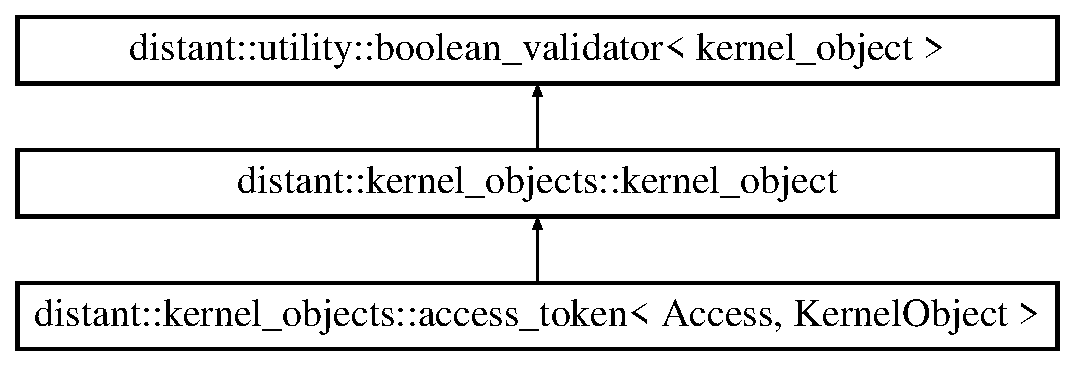
\includegraphics[height=3.000000cm]{classdistant_1_1kernel__objects_1_1access__token}
\end{center}
\end{figure}
\subsection*{Public Member Functions}
\begin{DoxyCompactItemize}
\item 
bool \mbox{\hyperlink{classdistant_1_1kernel__objects_1_1access__token_a6509ad02d8454898bdd591c6a70f55d5}{has\+\_\+privilege}} (const \mbox{\hyperlink{classdistant_1_1security_1_1privilege}{security\+::privilege}} \&p) const noexcept
\item 
bool \mbox{\hyperlink{classdistant_1_1kernel__objects_1_1access__token_aa51295b8d8f8602743d5d431806a29c4}{set\+\_\+privilege}} (const \mbox{\hyperlink{classdistant_1_1security_1_1privilege}{security\+::privilege}} \&p, security\+::privilege\+::attributes attribute=security\+::privilege\+::attributes\+::enabled) noexcept
\item 
bool \mbox{\hyperlink{classdistant_1_1kernel__objects_1_1access__token_aa396b0b32bd1f9aba79320a5104e0289}{remove\+\_\+privilege}} (const \mbox{\hyperlink{classdistant_1_1security_1_1privilege}{security\+::privilege}} \&p) noexcept
\item 
\mbox{\Hypertarget{classdistant_1_1kernel__objects_1_1access__token_a98db4be610792be51a07631bb3016a70}\label{classdistant_1_1kernel__objects_1_1access__token_a98db4be610792be51a07631bb3016a70}} 
{\bfseries access\+\_\+token} (const Kernel\+Object \&k) noexcept
\item 
\mbox{\Hypertarget{classdistant_1_1kernel__objects_1_1access__token_a9565c8e217a315df78664ef057b5fe18}\label{classdistant_1_1kernel__objects_1_1access__token_a9565c8e217a315df78664ef057b5fe18}} 
{\bfseries access\+\_\+token} (\mbox{\hyperlink{classdistant_1_1kernel__objects_1_1access__token}{access\+\_\+token}} \&\&) noexcept=default
\item 
\mbox{\Hypertarget{classdistant_1_1kernel__objects_1_1access__token_a095187fef9d7ec7297666e2eebff949c}\label{classdistant_1_1kernel__objects_1_1access__token_a095187fef9d7ec7297666e2eebff949c}} 
{\footnotesize template$<$access\+\_\+rights\+::token A, typename K $>$ }\\{\bfseries access\+\_\+token} (const K \&k) noexcept
\end{DoxyCompactItemize}
\subsection*{Friends}
\begin{DoxyCompactItemize}
\item 
\mbox{\Hypertarget{classdistant_1_1kernel__objects_1_1access__token_aae4643b98f37138b1f31ff510f3a3197}\label{classdistant_1_1kernel__objects_1_1access__token_aae4643b98f37138b1f31ff510f3a3197}} 
{\footnotesize template$<$access\+\_\+rights\+::token , class $>$ }\\class {\bfseries access\+\_\+token}
\end{DoxyCompactItemize}
\subsection*{Additional Inherited Members}


\subsection{Member Function Documentation}
\mbox{\Hypertarget{classdistant_1_1kernel__objects_1_1access__token_a6509ad02d8454898bdd591c6a70f55d5}\label{classdistant_1_1kernel__objects_1_1access__token_a6509ad02d8454898bdd591c6a70f55d5}} 
\index{distant\+::kernel\+\_\+objects\+::access\+\_\+token@{distant\+::kernel\+\_\+objects\+::access\+\_\+token}!has\+\_\+privilege@{has\+\_\+privilege}}
\index{has\+\_\+privilege@{has\+\_\+privilege}!distant\+::kernel\+\_\+objects\+::access\+\_\+token@{distant\+::kernel\+\_\+objects\+::access\+\_\+token}}
\subsubsection{\texorpdfstring{has\+\_\+privilege()}{has\_privilege()}}
{\footnotesize\ttfamily template$<$access\+\_\+rights\+::token A, typename K $>$ \\
bool \mbox{\hyperlink{classdistant_1_1kernel__objects_1_1access__token}{distant\+::kernel\+\_\+objects\+::access\+\_\+token}}$<$ A, K $>$\+::has\+\_\+privilege (\begin{DoxyParamCaption}\item[{const \mbox{\hyperlink{classdistant_1_1security_1_1privilege}{security\+::privilege}} \&}]{p }\end{DoxyParamCaption}) const\hspace{0.3cm}{\ttfamily [noexcept]}}

Check if the given privilege is in the access token\textquotesingle{}s list of privileges. 
\begin{DoxyParams}{Parameters}
{\em p} & the privilege to test. \\
\hline
\end{DoxyParams}
\begin{DoxyReturn}{Returns}
true if the privilege is enabled for the access token. 
\end{DoxyReturn}
\mbox{\Hypertarget{classdistant_1_1kernel__objects_1_1access__token_aa396b0b32bd1f9aba79320a5104e0289}\label{classdistant_1_1kernel__objects_1_1access__token_aa396b0b32bd1f9aba79320a5104e0289}} 
\index{distant\+::kernel\+\_\+objects\+::access\+\_\+token@{distant\+::kernel\+\_\+objects\+::access\+\_\+token}!remove\+\_\+privilege@{remove\+\_\+privilege}}
\index{remove\+\_\+privilege@{remove\+\_\+privilege}!distant\+::kernel\+\_\+objects\+::access\+\_\+token@{distant\+::kernel\+\_\+objects\+::access\+\_\+token}}
\subsubsection{\texorpdfstring{remove\+\_\+privilege()}{remove\_privilege()}}
{\footnotesize\ttfamily template$<$access\+\_\+rights\+::token A, typename K $>$ \\
bool \mbox{\hyperlink{classdistant_1_1kernel__objects_1_1access__token}{distant\+::kernel\+\_\+objects\+::access\+\_\+token}}$<$ A, K $>$\+::remove\+\_\+privilege (\begin{DoxyParamCaption}\item[{const \mbox{\hyperlink{classdistant_1_1security_1_1privilege}{security\+::privilege}} \&}]{p }\end{DoxyParamCaption})\hspace{0.3cm}{\ttfamily [noexcept]}}

Remove the given privilege from the access token. 
\begin{DoxyParams}{Parameters}
{\em p} & the privilege to remove. \\
\hline
\end{DoxyParams}
\begin{DoxyReturn}{Returns}
true if the privilege has been successfully removed. 
\end{DoxyReturn}
\mbox{\Hypertarget{classdistant_1_1kernel__objects_1_1access__token_aa51295b8d8f8602743d5d431806a29c4}\label{classdistant_1_1kernel__objects_1_1access__token_aa51295b8d8f8602743d5d431806a29c4}} 
\index{distant\+::kernel\+\_\+objects\+::access\+\_\+token@{distant\+::kernel\+\_\+objects\+::access\+\_\+token}!set\+\_\+privilege@{set\+\_\+privilege}}
\index{set\+\_\+privilege@{set\+\_\+privilege}!distant\+::kernel\+\_\+objects\+::access\+\_\+token@{distant\+::kernel\+\_\+objects\+::access\+\_\+token}}
\subsubsection{\texorpdfstring{set\+\_\+privilege()}{set\_privilege()}}
{\footnotesize\ttfamily template$<$access\+\_\+rights\+::token A, typename K $>$ \\
bool \mbox{\hyperlink{classdistant_1_1kernel__objects_1_1access__token}{distant\+::kernel\+\_\+objects\+::access\+\_\+token}}$<$ A, K $>$\+::set\+\_\+privilege (\begin{DoxyParamCaption}\item[{const \mbox{\hyperlink{classdistant_1_1security_1_1privilege}{security\+::privilege}} \&}]{p,  }\item[{security\+::privilege\+::attributes}]{attribute = {\ttfamily security\+:\+:privilege\+:\+:attributes\+:\+:enabled} }\end{DoxyParamCaption})\hspace{0.3cm}{\ttfamily [noexcept]}}

Enable/disable the given privilege in the access token 
\begin{DoxyParams}{Parameters}
{\em p} & the privilege to set. \\
\hline
{\em attribute} & enable, remove, or enable by default the privilege. \\
\hline
\end{DoxyParams}
\begin{DoxyReturn}{Returns}
true if the privilege has been successfully set. 
\end{DoxyReturn}


The documentation for this class was generated from the following files\+:\begin{DoxyCompactItemize}
\item 
C\+:/\+Users/dinne/source/repos/distant dev/distant dev/include/distant/kernel\+\_\+objects/access\+\_\+token.\+hpp\item 
C\+:/\+Users/dinne/source/repos/distant dev/distant dev/include/distant/kernel\+\_\+objects/impl/access\+\_\+token.\+hxx\end{DoxyCompactItemize}

\hypertarget{classdistant_1_1memory_1_1address}{}\section{distant\+:\+:memory\+:\+:address$<$ AddressT $>$ Class Template Reference}
\label{classdistant_1_1memory_1_1address}\index{distant\+::memory\+::address$<$ Address\+T $>$@{distant\+::memory\+::address$<$ Address\+T $>$}}
\subsection*{Public Types}
\begin{DoxyCompactItemize}
\item 
\mbox{\Hypertarget{classdistant_1_1memory_1_1address_ae7e5f3e881710ffeff16d4cc1187e3e5}\label{classdistant_1_1memory_1_1address_ae7e5f3e881710ffeff16d4cc1187e3e5}} 
using {\bfseries address\+\_\+type} = AddressT
\end{DoxyCompactItemize}
\subsection*{Public Member Functions}
\begin{DoxyCompactItemize}
\item 
\mbox{\Hypertarget{classdistant_1_1memory_1_1address_a1d0c5919b7d7397eb812b2f8ed7fb8fb}\label{classdistant_1_1memory_1_1address_a1d0c5919b7d7397eb812b2f8ed7fb8fb}} 
constexpr {\bfseries operator address\+\_\+type} () const noexcept
\item 
\mbox{\Hypertarget{classdistant_1_1memory_1_1address_a7563ca3df13cced36b6119b5582afb19}\label{classdistant_1_1memory_1_1address_a7563ca3df13cced36b6119b5582afb19}} 
constexpr \mbox{\hyperlink{classdistant_1_1memory_1_1address}{address}} \& {\bfseries operator+=} (\mbox{\hyperlink{classdistant_1_1memory_1_1address}{address}}) noexcept
\item 
\mbox{\Hypertarget{classdistant_1_1memory_1_1address_a11298753ba9b8825e0b5119dada37a4e}\label{classdistant_1_1memory_1_1address_a11298753ba9b8825e0b5119dada37a4e}} 
constexpr \mbox{\hyperlink{classdistant_1_1memory_1_1address}{address}} \& {\bfseries operator-\/=} (\mbox{\hyperlink{classdistant_1_1memory_1_1address}{address}}) noexcept
\item 
\mbox{\Hypertarget{classdistant_1_1memory_1_1address_aed59911560fdb1fe9ef50653f88ea39d}\label{classdistant_1_1memory_1_1address_aed59911560fdb1fe9ef50653f88ea39d}} 
constexpr \mbox{\hyperlink{classdistant_1_1memory_1_1address}{address}} \& {\bfseries operator$\ast$=} (\mbox{\hyperlink{classdistant_1_1memory_1_1address}{address}}) noexcept
\item 
\mbox{\Hypertarget{classdistant_1_1memory_1_1address_ab2f580751fb3e28fbed1762c660c0496}\label{classdistant_1_1memory_1_1address_ab2f580751fb3e28fbed1762c660c0496}} 
constexpr \mbox{\hyperlink{classdistant_1_1memory_1_1address}{address}} \& {\bfseries operator/=} (\mbox{\hyperlink{classdistant_1_1memory_1_1address}{address}}) noexcept
\item 
\mbox{\Hypertarget{classdistant_1_1memory_1_1address_a24e7114550241198b178a4d7f8f3a92a}\label{classdistant_1_1memory_1_1address_a24e7114550241198b178a4d7f8f3a92a}} 
constexpr \mbox{\hyperlink{classdistant_1_1memory_1_1address}{address}} \& {\bfseries operator\&=} (\mbox{\hyperlink{classdistant_1_1memory_1_1address}{address}}) noexcept
\item 
\mbox{\Hypertarget{classdistant_1_1memory_1_1address_accd05522a107b4180a08258bfdca5936}\label{classdistant_1_1memory_1_1address_accd05522a107b4180a08258bfdca5936}} 
constexpr \mbox{\hyperlink{classdistant_1_1memory_1_1address}{address}} \& {\bfseries operator$^\wedge$=} (\mbox{\hyperlink{classdistant_1_1memory_1_1address}{address}}) noexcept
\item 
\mbox{\Hypertarget{classdistant_1_1memory_1_1address_a920b0e3ae67efadeee2273ed1a3e3cd3}\label{classdistant_1_1memory_1_1address_a920b0e3ae67efadeee2273ed1a3e3cd3}} 
constexpr \mbox{\hyperlink{classdistant_1_1memory_1_1address}{address}} \& {\bfseries operator$\vert$=} (\mbox{\hyperlink{classdistant_1_1memory_1_1address}{address}}) noexcept
\item 
\mbox{\Hypertarget{classdistant_1_1memory_1_1address_adadb260d041b06f68a1bf827432e1918}\label{classdistant_1_1memory_1_1address_adadb260d041b06f68a1bf827432e1918}} 
{\footnotesize template$<$typename T $>$ }\\constexpr {\bfseries address} (T $\ast$x) noexcept
\item 
\mbox{\Hypertarget{classdistant_1_1memory_1_1address_a4dc4cad050aef738a19ebb63ed94e13d}\label{classdistant_1_1memory_1_1address_a4dc4cad050aef738a19ebb63ed94e13d}} 
constexpr {\bfseries address} (address\+\_\+type x) noexcept
\end{DoxyCompactItemize}
\subsection*{Friends}
\begin{DoxyCompactItemize}
\item 
\mbox{\Hypertarget{classdistant_1_1memory_1_1address_a8eefa780ab985fb77d69cbeaf4d82ad4}\label{classdistant_1_1memory_1_1address_a8eefa780ab985fb77d69cbeaf4d82ad4}} 
constexpr bool {\bfseries operator==} (const \mbox{\hyperlink{classdistant_1_1memory_1_1address}{address}} lhs, const \mbox{\hyperlink{classdistant_1_1memory_1_1address}{address}} rhs) noexcept
\item 
\mbox{\Hypertarget{classdistant_1_1memory_1_1address_ab78b2b70518bd59568ad03507bf938ae}\label{classdistant_1_1memory_1_1address_ab78b2b70518bd59568ad03507bf938ae}} 
constexpr bool {\bfseries operator$<$} (const \mbox{\hyperlink{classdistant_1_1memory_1_1address}{address}} lhs, const \mbox{\hyperlink{classdistant_1_1memory_1_1address}{address}} rhs) noexcept
\item 
\mbox{\Hypertarget{classdistant_1_1memory_1_1address_a2e154552a201f25abc0184f31afe1648}\label{classdistant_1_1memory_1_1address_a2e154552a201f25abc0184f31afe1648}} 
constexpr bool {\bfseries operator!=} (const \mbox{\hyperlink{classdistant_1_1memory_1_1address}{address}} lhs, const \mbox{\hyperlink{classdistant_1_1memory_1_1address}{address}} rhs) noexcept
\item 
\mbox{\Hypertarget{classdistant_1_1memory_1_1address_aa8dd8f3bdbeb0a68715bb8a824ed8257}\label{classdistant_1_1memory_1_1address_aa8dd8f3bdbeb0a68715bb8a824ed8257}} 
constexpr bool {\bfseries operator$>$=} (const \mbox{\hyperlink{classdistant_1_1memory_1_1address}{address}} lhs, const \mbox{\hyperlink{classdistant_1_1memory_1_1address}{address}} rhs) noexcept
\item 
\mbox{\Hypertarget{classdistant_1_1memory_1_1address_a6276259f2d9b36ecdd31a4d15754fd2a}\label{classdistant_1_1memory_1_1address_a6276259f2d9b36ecdd31a4d15754fd2a}} 
constexpr bool {\bfseries operator$>$} (const \mbox{\hyperlink{classdistant_1_1memory_1_1address}{address}} lhs, const \mbox{\hyperlink{classdistant_1_1memory_1_1address}{address}} rhs) noexcept
\item 
\mbox{\Hypertarget{classdistant_1_1memory_1_1address_a7a220d5b499d27f797a0bc5348270e86}\label{classdistant_1_1memory_1_1address_a7a220d5b499d27f797a0bc5348270e86}} 
constexpr bool {\bfseries operator$<$=} (const \mbox{\hyperlink{classdistant_1_1memory_1_1address}{address}} lhs, const \mbox{\hyperlink{classdistant_1_1memory_1_1address}{address}} rhs) noexcept
\item 
\mbox{\Hypertarget{classdistant_1_1memory_1_1address_aad3cc2980861b0dd81860ea54dc5fae1}\label{classdistant_1_1memory_1_1address_aad3cc2980861b0dd81860ea54dc5fae1}} 
constexpr \mbox{\hyperlink{classdistant_1_1memory_1_1address}{address}} {\bfseries operator\%} (const \mbox{\hyperlink{classdistant_1_1memory_1_1address}{address}} lhs, const \mbox{\hyperlink{classdistant_1_1memory_1_1address}{address}} rhs) noexcept
\item 
\mbox{\Hypertarget{classdistant_1_1memory_1_1address_a13dc3556cdaf1ea7ed0e912c18da3c6b}\label{classdistant_1_1memory_1_1address_a13dc3556cdaf1ea7ed0e912c18da3c6b}} 
constexpr \mbox{\hyperlink{classdistant_1_1memory_1_1address}{address}} {\bfseries operator \&} (const \mbox{\hyperlink{classdistant_1_1memory_1_1address}{address}} lhs, const \mbox{\hyperlink{classdistant_1_1memory_1_1address}{address}} rhs) noexcept
\item 
\mbox{\Hypertarget{classdistant_1_1memory_1_1address_ae9bebc2460e7e096f40a62965e4eb33f}\label{classdistant_1_1memory_1_1address_ae9bebc2460e7e096f40a62965e4eb33f}} 
constexpr \mbox{\hyperlink{classdistant_1_1memory_1_1address}{address}} {\bfseries operator$\vert$} (const \mbox{\hyperlink{classdistant_1_1memory_1_1address}{address}} lhs, const \mbox{\hyperlink{classdistant_1_1memory_1_1address}{address}} rhs) noexcept
\item 
\mbox{\Hypertarget{classdistant_1_1memory_1_1address_a48a9b10cf8ce09f2dc710181795fc18c}\label{classdistant_1_1memory_1_1address_a48a9b10cf8ce09f2dc710181795fc18c}} 
constexpr \mbox{\hyperlink{classdistant_1_1memory_1_1address}{address}} {\bfseries operator$^\wedge$} (const \mbox{\hyperlink{classdistant_1_1memory_1_1address}{address}} lhs, const \mbox{\hyperlink{classdistant_1_1memory_1_1address}{address}} rhs) noexcept
\item 
\mbox{\Hypertarget{classdistant_1_1memory_1_1address_a9845bd494e1520228fc261bd1d2f2d12}\label{classdistant_1_1memory_1_1address_a9845bd494e1520228fc261bd1d2f2d12}} 
constexpr \mbox{\hyperlink{classdistant_1_1memory_1_1address}{address}} {\bfseries operator$<$$<$} (const \mbox{\hyperlink{classdistant_1_1memory_1_1address}{address}} lhs, const \mbox{\hyperlink{classdistant_1_1memory_1_1address}{address}} rhs) noexcept
\item 
\mbox{\Hypertarget{classdistant_1_1memory_1_1address_a740cf28f126ed9d1956b3ef831e0fad6}\label{classdistant_1_1memory_1_1address_a740cf28f126ed9d1956b3ef831e0fad6}} 
constexpr \mbox{\hyperlink{classdistant_1_1memory_1_1address}{address}} {\bfseries operator$>$$>$} (const \mbox{\hyperlink{classdistant_1_1memory_1_1address}{address}} lhs, const \mbox{\hyperlink{classdistant_1_1memory_1_1address}{address}} rhs) noexcept
\item 
\mbox{\Hypertarget{classdistant_1_1memory_1_1address_a04953593dea9d095e38a4f515aef7d58}\label{classdistant_1_1memory_1_1address_a04953593dea9d095e38a4f515aef7d58}} 
constexpr \mbox{\hyperlink{classdistant_1_1memory_1_1address}{address}} {\bfseries operator+} (const \mbox{\hyperlink{classdistant_1_1memory_1_1address}{address}} lhs, const \mbox{\hyperlink{classdistant_1_1memory_1_1address}{address}} rhs) noexcept
\item 
\mbox{\Hypertarget{classdistant_1_1memory_1_1address_ab7b9a651b5cf91cdc4faad61e42752c2}\label{classdistant_1_1memory_1_1address_ab7b9a651b5cf91cdc4faad61e42752c2}} 
constexpr \mbox{\hyperlink{classdistant_1_1memory_1_1address}{address}} {\bfseries operator-\/} (const \mbox{\hyperlink{classdistant_1_1memory_1_1address}{address}} lhs, const \mbox{\hyperlink{classdistant_1_1memory_1_1address}{address}} rhs) noexcept
\item 
\mbox{\Hypertarget{classdistant_1_1memory_1_1address_a4e614d2c07d4570fb6e96e6d0d1399c9}\label{classdistant_1_1memory_1_1address_a4e614d2c07d4570fb6e96e6d0d1399c9}} 
constexpr \mbox{\hyperlink{classdistant_1_1memory_1_1address}{address}} {\bfseries operator$\ast$} (const \mbox{\hyperlink{classdistant_1_1memory_1_1address}{address}} lhs, const \mbox{\hyperlink{classdistant_1_1memory_1_1address}{address}} rhs) noexcept
\item 
\mbox{\Hypertarget{classdistant_1_1memory_1_1address_adfaca89e0f2970dc529f38052fb4db79}\label{classdistant_1_1memory_1_1address_adfaca89e0f2970dc529f38052fb4db79}} 
constexpr \mbox{\hyperlink{classdistant_1_1memory_1_1address}{address}} {\bfseries operator/} (const \mbox{\hyperlink{classdistant_1_1memory_1_1address}{address}} lhs, const \mbox{\hyperlink{classdistant_1_1memory_1_1address}{address}} rhs) noexcept
\end{DoxyCompactItemize}


The documentation for this class was generated from the following files\+:\begin{DoxyCompactItemize}
\item 
C\+:/\+Users/dinne/source/repos/distant dev/distant dev/include/distant/memory/address.\+hpp\item 
C\+:/\+Users/dinne/source/repos/distant dev/distant dev/include/distant/memory/impl/address.\+hxx\end{DoxyCompactItemize}

\hypertarget{classaddress__space}{}\section{address\+\_\+space Class Reference}
\label{classaddress__space}\index{address\+\_\+space@{address\+\_\+space}}


The documentation for this class was generated from the following file\+:\begin{DoxyCompactItemize}
\item 
C\+:/\+Users/dinne/source/repos/distant dev/distant dev/include/distant/memory/address\+\_\+space.\+hpp\end{DoxyCompactItemize}

\hypertarget{structdistant_1_1function__traits_3_01function_3_01_r_07_args_8_8_8_08_00_01_calling_conv_00_01_address_t_01_4_01_4_1_1argument}{}\section{distant\+:\+:function\+\_\+traits$<$ function$<$ R(Args...), Calling\+Conv, AddressT $>$ $>$\+:\+:argument$<$ N $>$ Struct Template Reference}
\label{structdistant_1_1function__traits_3_01function_3_01_r_07_args_8_8_8_08_00_01_calling_conv_00_01_address_t_01_4_01_4_1_1argument}\index{distant\+::function\+\_\+traits$<$ function$<$ R(\+Args...), Calling\+Conv, Address\+T $>$ $>$\+::argument$<$ N $>$@{distant\+::function\+\_\+traits$<$ function$<$ R(\+Args...), Calling\+Conv, Address\+T $>$ $>$\+::argument$<$ N $>$}}
\subsection*{Public Types}
\begin{DoxyCompactItemize}
\item 
\mbox{\Hypertarget{structdistant_1_1function__traits_3_01function_3_01_r_07_args_8_8_8_08_00_01_calling_conv_00_01_address_t_01_4_01_4_1_1argument_a227914de4a3cd9b3b25f181fe6b1010e}\label{structdistant_1_1function__traits_3_01function_3_01_r_07_args_8_8_8_08_00_01_calling_conv_00_01_address_t_01_4_01_4_1_1argument_a227914de4a3cd9b3b25f181fe6b1010e}} 
using {\bfseries type} = std\+::tuple\+\_\+element\+\_\+t$<$ N, std\+::tuple$<$ Args... $>$ $>$
\end{DoxyCompactItemize}


The documentation for this struct was generated from the following file\+:\begin{DoxyCompactItemize}
\item 
C\+:/\+Users/dinne/source/repos/distant dev/distant dev/include/distant/memory/function.\+hpp\end{DoxyCompactItemize}

\hypertarget{classdistant_1_1utility_1_1boolean__validator}{}\section{distant\+:\+:utility\+:\+:boolean\+\_\+validator$<$ Derived $>$ Class Template Reference}
\label{classdistant_1_1utility_1_1boolean__validator}\index{distant\+::utility\+::boolean\+\_\+validator$<$ Derived $>$@{distant\+::utility\+::boolean\+\_\+validator$<$ Derived $>$}}
\subsection*{Public Member Functions}
\begin{DoxyCompactItemize}
\item 
\mbox{\Hypertarget{classdistant_1_1utility_1_1boolean__validator_a4b549ffb8fddc68ec7370bb3df93f7d3}\label{classdistant_1_1utility_1_1boolean__validator_a4b549ffb8fddc68ec7370bb3df93f7d3}} 
{\bfseries operator bool} () const noexcept
\end{DoxyCompactItemize}


The documentation for this class was generated from the following file\+:\begin{DoxyCompactItemize}
\item 
C\+:/\+Users/dinne/source/repos/distant dev/distant dev/include/distant/utility/boolean\+\_\+validator.\+hpp\end{DoxyCompactItemize}

\hypertarget{structdistant_1_1memory_1_1x86__calling__conventions_1_1cdeclcall}{}\section{distant\+:\+:memory\+:\+:x86\+\_\+calling\+\_\+conventions\+:\+:cdeclcall Struct Reference}
\label{structdistant_1_1memory_1_1x86__calling__conventions_1_1cdeclcall}\index{distant\+::memory\+::x86\+\_\+calling\+\_\+conventions\+::cdeclcall@{distant\+::memory\+::x86\+\_\+calling\+\_\+conventions\+::cdeclcall}}


The documentation for this struct was generated from the following file\+:\begin{DoxyCompactItemize}
\item 
C\+:/\+Users/dinne/source/repos/distant dev/distant dev/include/distant/memory/x86\+\_\+calling\+\_\+conventions.\+hpp\end{DoxyCompactItemize}

\hypertarget{structdistant_1_1utility_1_1detail_1_1detector}{}\section{distant\+:\+:utility\+:\+:detail\+:\+:detector$<$ Default, Always\+Void, Op, Args $>$ Struct Template Reference}
\label{structdistant_1_1utility_1_1detail_1_1detector}\index{distant\+::utility\+::detail\+::detector$<$ Default, Always\+Void, Op, Args $>$@{distant\+::utility\+::detail\+::detector$<$ Default, Always\+Void, Op, Args $>$}}
\subsection*{Public Types}
\begin{DoxyCompactItemize}
\item 
\mbox{\Hypertarget{structdistant_1_1utility_1_1detail_1_1detector_a66286f0f6fe1b7c5a8aa2b0300fc3143}\label{structdistant_1_1utility_1_1detail_1_1detector_a66286f0f6fe1b7c5a8aa2b0300fc3143}} 
using {\bfseries value\+\_\+t} = std\+::false\+\_\+type
\item 
\mbox{\Hypertarget{structdistant_1_1utility_1_1detail_1_1detector_a1b5495d07d6b5969a68dbfd48c9e5b8e}\label{structdistant_1_1utility_1_1detail_1_1detector_a1b5495d07d6b5969a68dbfd48c9e5b8e}} 
using {\bfseries type} = Default
\end{DoxyCompactItemize}


The documentation for this struct was generated from the following file\+:\begin{DoxyCompactItemize}
\item 
C\+:/\+Users/dinne/source/repos/distant dev/distant dev/include/distant/utility/detection.\+hpp\end{DoxyCompactItemize}

\hypertarget{structdistant_1_1utility_1_1detail_1_1detector_3_01_default_00_01std_1_1void__t_3_01_op_3_01_arg04e1ee669e2093134af6db72a2dfc0d6}{}\section{distant\+:\+:utility\+:\+:detail\+:\+:detector$<$ Default, std\+:\+:void\+\_\+t$<$ Op$<$ Args... $>$ $>$, Op, Args... $>$ Struct Template Reference}
\label{structdistant_1_1utility_1_1detail_1_1detector_3_01_default_00_01std_1_1void__t_3_01_op_3_01_arg04e1ee669e2093134af6db72a2dfc0d6}\index{distant\+::utility\+::detail\+::detector$<$ Default, std\+::void\+\_\+t$<$ Op$<$ Args... $>$ $>$, Op, Args... $>$@{distant\+::utility\+::detail\+::detector$<$ Default, std\+::void\+\_\+t$<$ Op$<$ Args... $>$ $>$, Op, Args... $>$}}
\subsection*{Public Types}
\begin{DoxyCompactItemize}
\item 
\mbox{\Hypertarget{structdistant_1_1utility_1_1detail_1_1detector_3_01_default_00_01std_1_1void__t_3_01_op_3_01_arg04e1ee669e2093134af6db72a2dfc0d6_af0de3097b60600cc721bfb00e3ed5b18}\label{structdistant_1_1utility_1_1detail_1_1detector_3_01_default_00_01std_1_1void__t_3_01_op_3_01_arg04e1ee669e2093134af6db72a2dfc0d6_af0de3097b60600cc721bfb00e3ed5b18}} 
using {\bfseries value\+\_\+t} = std\+::true\+\_\+type
\item 
\mbox{\Hypertarget{structdistant_1_1utility_1_1detail_1_1detector_3_01_default_00_01std_1_1void__t_3_01_op_3_01_arg04e1ee669e2093134af6db72a2dfc0d6_acefbdcfec94395ff7cb144c8283033da}\label{structdistant_1_1utility_1_1detail_1_1detector_3_01_default_00_01std_1_1void__t_3_01_op_3_01_arg04e1ee669e2093134af6db72a2dfc0d6_acefbdcfec94395ff7cb144c8283033da}} 
using {\bfseries type} = Op$<$ Args... $>$
\end{DoxyCompactItemize}


The documentation for this struct was generated from the following file\+:\begin{DoxyCompactItemize}
\item 
C\+:/\+Users/dinne/source/repos/distant dev/distant dev/include/distant/utility/detection.\+hpp\end{DoxyCompactItemize}

\hypertarget{structdistant_1_1kernel__objects_1_1detail_1_1dispatcher}{}\section{distant\+:\+:kernel\+\_\+objects\+:\+:detail\+:\+:dispatcher$<$ Object $>$ Struct Template Reference}
\label{structdistant_1_1kernel__objects_1_1detail_1_1dispatcher}\index{distant\+::kernel\+\_\+objects\+::detail\+::dispatcher$<$ Object $>$@{distant\+::kernel\+\_\+objects\+::detail\+::dispatcher$<$ Object $>$}}


The documentation for this struct was generated from the following file\+:\begin{DoxyCompactItemize}
\item 
C\+:/\+Users/dinne/source/repos/distant dev/distant dev/include/distant/kernel\+\_\+objects/impl/access\+\_\+token.\+hxx\end{DoxyCompactItemize}

\hypertarget{structdistant_1_1kernel__objects_1_1detail_1_1dispatcher_3_01process_3_01_a_01_4_01_4}{}\section{distant\+:\+:kernel\+\_\+objects\+:\+:detail\+:\+:dispatcher$<$ process$<$ A $>$ $>$ Struct Template Reference}
\label{structdistant_1_1kernel__objects_1_1detail_1_1dispatcher_3_01process_3_01_a_01_4_01_4}\index{distant\+::kernel\+\_\+objects\+::detail\+::dispatcher$<$ process$<$ A $>$ $>$@{distant\+::kernel\+\_\+objects\+::detail\+::dispatcher$<$ process$<$ A $>$ $>$}}
\subsection*{Public Types}
\begin{DoxyCompactItemize}
\item 
\mbox{\Hypertarget{structdistant_1_1kernel__objects_1_1detail_1_1dispatcher_3_01process_3_01_a_01_4_01_4_a6670f8e129f24d1a1dd143dcda0b625e}\label{structdistant_1_1kernel__objects_1_1detail_1_1dispatcher_3_01process_3_01_a_01_4_01_4_a6670f8e129f24d1a1dd143dcda0b625e}} 
using {\bfseries dispatch} = \mbox{\hyperlink{classdistant_1_1detail_1_1process__tag}{distant\+::detail\+::process\+\_\+tag}}
\end{DoxyCompactItemize}


The documentation for this struct was generated from the following file\+:\begin{DoxyCompactItemize}
\item 
C\+:/\+Users/dinne/source/repos/distant dev/distant dev/include/distant/kernel\+\_\+objects/impl/access\+\_\+token.\+hxx\end{DoxyCompactItemize}

\hypertarget{structdistant_1_1kernel__objects_1_1detail_1_1dispatcher_3_01process__base_01_4}{}\section{distant\+:\+:kernel\+\_\+objects\+:\+:detail\+:\+:dispatcher$<$ process\+\_\+base $>$ Struct Template Reference}
\label{structdistant_1_1kernel__objects_1_1detail_1_1dispatcher_3_01process__base_01_4}\index{distant\+::kernel\+\_\+objects\+::detail\+::dispatcher$<$ process\+\_\+base $>$@{distant\+::kernel\+\_\+objects\+::detail\+::dispatcher$<$ process\+\_\+base $>$}}
\subsection*{Public Types}
\begin{DoxyCompactItemize}
\item 
\mbox{\Hypertarget{structdistant_1_1kernel__objects_1_1detail_1_1dispatcher_3_01process__base_01_4_a8720cc8d4df1f497c3b4c17c109af8c0}\label{structdistant_1_1kernel__objects_1_1detail_1_1dispatcher_3_01process__base_01_4_a8720cc8d4df1f497c3b4c17c109af8c0}} 
using {\bfseries dispatch} = \mbox{\hyperlink{classdistant_1_1detail_1_1process__base__tag}{distant\+::detail\+::process\+\_\+base\+\_\+tag}}
\end{DoxyCompactItemize}


The documentation for this struct was generated from the following file\+:\begin{DoxyCompactItemize}
\item 
C\+:/\+Users/dinne/source/repos/distant dev/distant dev/include/distant/kernel\+\_\+objects/impl/access\+\_\+token.\+hxx\end{DoxyCompactItemize}

\hypertarget{structdistant_1_1assembly_1_1dword__ptr__t}{}\section{distant\+:\+:assembly\+:\+:dword\+\_\+ptr\+\_\+t$<$ T, typename $>$ Struct Template Reference}
\label{structdistant_1_1assembly_1_1dword__ptr__t}\index{distant\+::assembly\+::dword\+\_\+ptr\+\_\+t$<$ T, typename $>$@{distant\+::assembly\+::dword\+\_\+ptr\+\_\+t$<$ T, typename $>$}}
\subsection*{Public Member Functions}
\begin{DoxyCompactItemize}
\item 
\mbox{\Hypertarget{structdistant_1_1assembly_1_1dword__ptr__t_ac9e3696a6fed8f916403264c5ec7de75}\label{structdistant_1_1assembly_1_1dword__ptr__t_ac9e3696a6fed8f916403264c5ec7de75}} 
constexpr {\bfseries dword\+\_\+ptr\+\_\+t} (T reg\+\_\+address) noexcept
\end{DoxyCompactItemize}
\subsection*{Public Attributes}
\begin{DoxyCompactItemize}
\item 
\mbox{\Hypertarget{structdistant_1_1assembly_1_1dword__ptr__t_afad65828b73d9a40e84777aeae76a2d9}\label{structdistant_1_1assembly_1_1dword__ptr__t_afad65828b73d9a40e84777aeae76a2d9}} 
T {\bfseries data}
\end{DoxyCompactItemize}


The documentation for this struct was generated from the following files\+:\begin{DoxyCompactItemize}
\item 
C\+:/\+Users/dinne/source/repos/distant dev/distant dev/include/distant/assembly/dword\+\_\+ptr.\+hpp\item 
C\+:/\+Users/dinne/source/repos/distant dev/distant dev/include/distant/assembly/impl/dword\+\_\+ptr.\+hxx\end{DoxyCompactItemize}

\hypertarget{structdistant_1_1memory_1_1x86__calling__conventions_1_1fastcall}{}\section{distant\+:\+:memory\+:\+:x86\+\_\+calling\+\_\+conventions\+:\+:fastcall Struct Reference}
\label{structdistant_1_1memory_1_1x86__calling__conventions_1_1fastcall}\index{distant\+::memory\+::x86\+\_\+calling\+\_\+conventions\+::fastcall@{distant\+::memory\+::x86\+\_\+calling\+\_\+conventions\+::fastcall}}


The documentation for this struct was generated from the following file\+:\begin{DoxyCompactItemize}
\item 
C\+:/\+Users/dinne/source/repos/distant dev/distant dev/include/distant/memory/x86\+\_\+calling\+\_\+conventions.\+hpp\end{DoxyCompactItemize}

\hypertarget{classdistant_1_1memory_1_1function}{}\section{distant\+:\+:memory\+:\+:function$<$ Signature, Calling\+Conv, AddressT $>$ Class Template Reference}
\label{classdistant_1_1memory_1_1function}\index{distant\+::memory\+::function$<$ Signature, Calling\+Conv, Address\+T $>$@{distant\+::memory\+::function$<$ Signature, Calling\+Conv, Address\+T $>$}}


The documentation for this class was generated from the following file\+:\begin{DoxyCompactItemize}
\item 
C\+:/\+Users/dinne/source/repos/distant dev/distant dev/include/distant/memory/function.\+hpp\end{DoxyCompactItemize}

\hypertarget{classdistant_1_1memory_1_1function_3_01_r_07_args_8_8_8_08_00_01_calling_conv_00_01_address_t_01_4}{}\section{distant\+:\+:memory\+:\+:function$<$ R(Args...), Calling\+Conv, AddressT $>$ Class Template Reference}
\label{classdistant_1_1memory_1_1function_3_01_r_07_args_8_8_8_08_00_01_calling_conv_00_01_address_t_01_4}\index{distant\+::memory\+::function$<$ R(\+Args...), Calling\+Conv, Address\+T $>$@{distant\+::memory\+::function$<$ R(\+Args...), Calling\+Conv, Address\+T $>$}}
\subsection*{Public Member Functions}
\begin{DoxyCompactItemize}
\item 
\mbox{\Hypertarget{classdistant_1_1memory_1_1function_3_01_r_07_args_8_8_8_08_00_01_calling_conv_00_01_address_t_01_4_acbda97a4a9bb552c1975344651e7918e}\label{classdistant_1_1memory_1_1function_3_01_r_07_args_8_8_8_08_00_01_calling_conv_00_01_address_t_01_4_acbda97a4a9bb552c1975344651e7918e}} 
{\bfseries function} (\mbox{\hyperlink{classdistant_1_1memory_1_1virtual__ptr}{virtual\+\_\+ptr}}$<$ R($\ast$)(Args...), AddressT $>$ fn\+\_\+ptr)
\item 
\mbox{\Hypertarget{classdistant_1_1memory_1_1function_3_01_r_07_args_8_8_8_08_00_01_calling_conv_00_01_address_t_01_4_a611d9de83f572c092ef421fb59abc400}\label{classdistant_1_1memory_1_1function_3_01_r_07_args_8_8_8_08_00_01_calling_conv_00_01_address_t_01_4_a611d9de83f572c092ef421fb59abc400}} 
R {\bfseries operator()} (Args... args)
\item 
\mbox{\Hypertarget{classdistant_1_1memory_1_1function_3_01_r_07_args_8_8_8_08_00_01_calling_conv_00_01_address_t_01_4_aa3e56a849a300645283d8a36f3ee31b6}\label{classdistant_1_1memory_1_1function_3_01_r_07_args_8_8_8_08_00_01_calling_conv_00_01_address_t_01_4_aa3e56a849a300645283d8a36f3ee31b6}} 
void {\bfseries set\+\_\+process} (const \mbox{\hyperlink{classdistant_1_1kernel__objects_1_1process}{process}}$<$ required\+\_\+process\+\_\+rights $>$ \&\mbox{\hyperlink{classdistant_1_1kernel__objects_1_1process}{process}}) noexcept
\end{DoxyCompactItemize}
\subsection*{Static Public Attributes}
\begin{DoxyCompactItemize}
\item 
\mbox{\Hypertarget{classdistant_1_1memory_1_1function_3_01_r_07_args_8_8_8_08_00_01_calling_conv_00_01_address_t_01_4_ab07fcaedbf8783ee5ab8be04c883019a}\label{classdistant_1_1memory_1_1function_3_01_r_07_args_8_8_8_08_00_01_calling_conv_00_01_address_t_01_4_ab07fcaedbf8783ee5ab8be04c883019a}} 
static constexpr auto {\bfseries required\+\_\+process\+\_\+rights} = process\+\_\+rights\+::all\+\_\+access
\end{DoxyCompactItemize}


The documentation for this class was generated from the following file\+:\begin{DoxyCompactItemize}
\item 
C\+:/\+Users/dinne/source/repos/distant dev/distant dev/include/distant/memory/function.\+hpp\end{DoxyCompactItemize}

\hypertarget{structdistant_1_1function__traits}{}\section{distant\+:\+:function\+\_\+traits$<$ F $>$ Struct Template Reference}
\label{structdistant_1_1function__traits}\index{distant\+::function\+\_\+traits$<$ F $>$@{distant\+::function\+\_\+traits$<$ F $>$}}


The documentation for this struct was generated from the following file\+:\begin{DoxyCompactItemize}
\item 
C\+:/\+Users/dinne/source/repos/distant dev/distant dev/include/distant/memory/type\+\_\+traits.\+hpp\end{DoxyCompactItemize}

\hypertarget{structdistant_1_1function__traits_3_01function_3_01_r_07_args_8_8_8_08_00_01_calling_conv_00_01_address_t_01_4_01_4}{}\section{distant\+:\+:function\+\_\+traits$<$ function$<$ R(Args...), Calling\+Conv, AddressT $>$ $>$ Struct Template Reference}
\label{structdistant_1_1function__traits_3_01function_3_01_r_07_args_8_8_8_08_00_01_calling_conv_00_01_address_t_01_4_01_4}\index{distant\+::function\+\_\+traits$<$ function$<$ R(\+Args...), Calling\+Conv, Address\+T $>$ $>$@{distant\+::function\+\_\+traits$<$ function$<$ R(\+Args...), Calling\+Conv, Address\+T $>$ $>$}}
\subsection*{Classes}
\begin{DoxyCompactItemize}
\item 
struct \mbox{\hyperlink{structdistant_1_1function__traits_3_01function_3_01_r_07_args_8_8_8_08_00_01_calling_conv_00_01_address_t_01_4_01_4_1_1argument}{argument}}
\end{DoxyCompactItemize}
\subsection*{Public Types}
\begin{DoxyCompactItemize}
\item 
\mbox{\Hypertarget{structdistant_1_1function__traits_3_01function_3_01_r_07_args_8_8_8_08_00_01_calling_conv_00_01_address_t_01_4_01_4_a9cf34c74c3f6646f85274e0c5a23a505}\label{structdistant_1_1function__traits_3_01function_3_01_r_07_args_8_8_8_08_00_01_calling_conv_00_01_address_t_01_4_01_4_a9cf34c74c3f6646f85274e0c5a23a505}} 
using {\bfseries return\+\_\+type} = R
\item 
\mbox{\Hypertarget{structdistant_1_1function__traits_3_01function_3_01_r_07_args_8_8_8_08_00_01_calling_conv_00_01_address_t_01_4_01_4_a89d90414bcba6d493ef77f618e418aa5}\label{structdistant_1_1function__traits_3_01function_3_01_r_07_args_8_8_8_08_00_01_calling_conv_00_01_address_t_01_4_01_4_a89d90414bcba6d493ef77f618e418aa5}} 
{\footnotesize template$<$unsigned int N$>$ }\\using {\bfseries argument\+\_\+t} = typename argument$<$ N $>$\+::type
\end{DoxyCompactItemize}
\subsection*{Static Public Attributes}
\begin{DoxyCompactItemize}
\item 
\mbox{\Hypertarget{structdistant_1_1function__traits_3_01function_3_01_r_07_args_8_8_8_08_00_01_calling_conv_00_01_address_t_01_4_01_4_a27160e4e8828b01f03753094e132a1fd}\label{structdistant_1_1function__traits_3_01function_3_01_r_07_args_8_8_8_08_00_01_calling_conv_00_01_address_t_01_4_01_4_a27160e4e8828b01f03753094e132a1fd}} 
static constexpr std\+::size\+\_\+t {\bfseries arity} = sizeof...(Args)
\end{DoxyCompactItemize}


The documentation for this struct was generated from the following file\+:\begin{DoxyCompactItemize}
\item 
C\+:/\+Users/dinne/source/repos/distant dev/distant dev/include/distant/memory/function.\+hpp\end{DoxyCompactItemize}

\hypertarget{structdistant_1_1get__access__rights}{}\section{distant\+:\+:get\+\_\+access\+\_\+rights$<$ Object $>$ Struct Template Reference}
\label{structdistant_1_1get__access__rights}\index{distant\+::get\+\_\+access\+\_\+rights$<$ Object $>$@{distant\+::get\+\_\+access\+\_\+rights$<$ Object $>$}}


The documentation for this struct was generated from the following file\+:\begin{DoxyCompactItemize}
\item 
C\+:/\+Users/dinne/source/repos/distant dev/distant dev/include/distant/type\+\_\+traits.\+hpp\end{DoxyCompactItemize}

\hypertarget{structdistant_1_1get__access__rights_3_01kernel__objects_1_1process_3_01_access_01_4_01_4}{}\section{distant\+:\+:get\+\_\+access\+\_\+rights$<$ kernel\+\_\+objects\+:\+:process$<$ Access $>$ $>$ Struct Template Reference}
\label{structdistant_1_1get__access__rights_3_01kernel__objects_1_1process_3_01_access_01_4_01_4}\index{distant\+::get\+\_\+access\+\_\+rights$<$ kernel\+\_\+objects\+::process$<$ Access $>$ $>$@{distant\+::get\+\_\+access\+\_\+rights$<$ kernel\+\_\+objects\+::process$<$ Access $>$ $>$}}
\subsection*{Static Public Attributes}
\begin{DoxyCompactItemize}
\item 
\mbox{\Hypertarget{structdistant_1_1get__access__rights_3_01kernel__objects_1_1process_3_01_access_01_4_01_4_a3d0fb6e2482b01322d332af09eecb34c}\label{structdistant_1_1get__access__rights_3_01kernel__objects_1_1process_3_01_access_01_4_01_4_a3d0fb6e2482b01322d332af09eecb34c}} 
static constexpr auto {\bfseries value} = Access
\end{DoxyCompactItemize}


The documentation for this struct was generated from the following file\+:\begin{DoxyCompactItemize}
\item 
C\+:/\+Users/dinne/source/repos/distant dev/distant dev/include/distant/kernel\+\_\+objects/process.\+hpp\end{DoxyCompactItemize}

\hypertarget{structdistant_1_1error_1_1gle}{}\section{distant\+:\+:error\+:\+:gle Struct Reference}
\label{structdistant_1_1error_1_1gle}\index{distant\+::error\+::gle@{distant\+::error\+::gle}}


The documentation for this struct was generated from the following file\+:\begin{DoxyCompactItemize}
\item 
C\+:/\+Users/dinne/source/repos/distant dev/distant dev/include/distant/error/windows\+\_\+error.\+hpp\end{DoxyCompactItemize}

\hypertarget{classdistant_1_1handle}{}\section{distant\+:\+:handle$<$ ObjectT $>$ Class Template Reference}
\label{classdistant_1_1handle}\index{distant\+::handle$<$ Object\+T $>$@{distant\+::handle$<$ Object\+T $>$}}


Type-\/safe handle for windows objects.  




{\ttfamily \#include $<$handle.\+hpp$>$}

Inheritance diagram for distant\+:\+:handle$<$ ObjectT $>$\+:\begin{figure}[H]
\begin{center}
\leavevmode
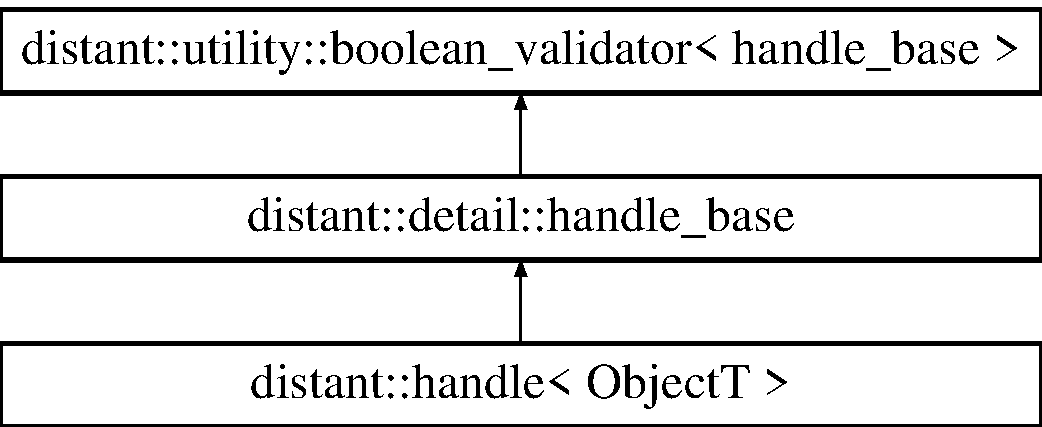
\includegraphics[height=3.000000cm]{classdistant_1_1handle}
\end{center}
\end{figure}
\subsection*{Public Types}
\begin{DoxyCompactItemize}
\item 
\mbox{\Hypertarget{classdistant_1_1handle_ad0687033839123a1babb00fd9d3735e9}\label{classdistant_1_1handle_ad0687033839123a1babb00fd9d3735e9}} 
using {\bfseries object\+\_\+type} = ObjectT
\end{DoxyCompactItemize}
\subsection*{Public Member Functions}
\begin{DoxyCompactItemize}
\item 
constexpr \mbox{\hyperlink{classdistant_1_1handle_a62c90d8be9b15cce2e0ec0ac85aab687}{handle}} (native\+\_\+type \mbox{\hyperlink{classdistant_1_1detail_1_1handle__base_a3207e125c17f2ebb59cab614083f782b}{native\+\_\+handle}}, flag\+\_\+type \mbox{\hyperlink{classdistant_1_1detail_1_1handle__base_adc97dc91543d76d0b89f43fee5f5f26b}{flags}}=flag\+\_\+type\+::inherit, bool \mbox{\hyperlink{classdistant_1_1detail_1_1handle__base_abd5ad44b32fda79418c5faada682336a}{closed}}=false) noexcept
\item 
constexpr \mbox{\hyperlink{classdistant_1_1handle_af2f4a42da3e2c88b0593cefa439e20ed}{handle}} (nullptr\+\_\+t h) noexcept
\item 
\mbox{\Hypertarget{classdistant_1_1handle_a05cdf625487c59ffdfee11470fad5d41}\label{classdistant_1_1handle_a05cdf625487c59ffdfee11470fad5d41}} 
constexpr \mbox{\hyperlink{classdistant_1_1handle_a05cdf625487c59ffdfee11470fad5d41}{handle}} () noexcept
\begin{DoxyCompactList}\small\item\em Invalid handle literal constructor. \end{DoxyCompactList}\item 
\mbox{\Hypertarget{classdistant_1_1handle_ae4a3ee70142af4ac84eab8542e4cac17}\label{classdistant_1_1handle_ae4a3ee70142af4ac84eab8542e4cac17}} 
{\footnotesize template$<$typename OtherT , typename  = std\+::enable\+\_\+if\+\_\+t$<$is\+\_\+quasiconvertible$<$\+Object\+T, Other\+T$>$\+::value$>$$>$ }\\{\bfseries handle} (\mbox{\hyperlink{classdistant_1_1handle}{handle}}$<$ OtherT $>$ \&\&other) noexcept
\item 
\mbox{\Hypertarget{classdistant_1_1handle_a4d6d2690a64a8105236d236168f60f1c}\label{classdistant_1_1handle_a4d6d2690a64a8105236d236168f60f1c}} 
{\footnotesize template$<$typename OtherT , typename  = std\+::enable\+\_\+if\+\_\+t$<$is\+\_\+quasiconvertible$<$\+Object\+T, Other\+T$>$\+::value$>$$>$ }\\\mbox{\hyperlink{classdistant_1_1handle}{handle}} \& {\bfseries operator=} (\mbox{\hyperlink{classdistant_1_1handle}{handle}}$<$ OtherT $>$ \&\&) noexcept
\item 
\mbox{\Hypertarget{classdistant_1_1handle_a1aeeca85db91bd5c1596f2c79680315f}\label{classdistant_1_1handle_a1aeeca85db91bd5c1596f2c79680315f}} 
{\bfseries handle} (\mbox{\hyperlink{classdistant_1_1handle}{handle}} \&\&) noexcept=default
\item 
\mbox{\Hypertarget{classdistant_1_1handle_a74bb937d5bd3f82a1bbf96d4fa2202cb}\label{classdistant_1_1handle_a74bb937d5bd3f82a1bbf96d4fa2202cb}} 
\mbox{\hyperlink{classdistant_1_1handle}{handle}} \& {\bfseries operator=} (\mbox{\hyperlink{classdistant_1_1handle}{handle}} \&\&) noexcept=default
\item 
\mbox{\Hypertarget{classdistant_1_1handle_a8bcd9d7f086f2f2660ff1864cbd21989}\label{classdistant_1_1handle_a8bcd9d7f086f2f2660ff1864cbd21989}} 
{\footnotesize template$<$typename U $>$ }\\void {\bfseries swap} (\mbox{\hyperlink{classdistant_1_1handle}{handle}}$<$ U $>$ \&other) noexcept
\item 
\mbox{\Hypertarget{classdistant_1_1handle_a5c2bed1faa6a28060e9090fdc9536fd3}\label{classdistant_1_1handle_a5c2bed1faa6a28060e9090fdc9536fd3}} 
{\footnotesize template$<$typename OtherT , typename $>$ }\\\mbox{\hyperlink{classdistant_1_1handle}{handle}}$<$ T $>$ \& {\bfseries operator=} (\mbox{\hyperlink{classdistant_1_1handle}{handle}}$<$ OtherT $>$ \&\&other) noexcept
\end{DoxyCompactItemize}
\subsection*{Friends}
\begin{DoxyCompactItemize}
\item 
\mbox{\Hypertarget{classdistant_1_1handle_a09563db836b1abb27abbd07b38d77cf7}\label{classdistant_1_1handle_a09563db836b1abb27abbd07b38d77cf7}} 
{\footnotesize template$<$typename $>$ }\\class {\bfseries handle}
\item 
\mbox{\Hypertarget{classdistant_1_1handle_aa0ed784cab3502540e32427581986e33}\label{classdistant_1_1handle_aa0ed784cab3502540e32427581986e33}} 
{\footnotesize template$<$typename T , typename U $>$ }\\constexpr bool {\bfseries operator==} (const \mbox{\hyperlink{classdistant_1_1handle}{handle}}$<$ T $>$ \&, const \mbox{\hyperlink{classdistant_1_1handle}{handle}}$<$ U $>$ \&) noexcept
\item 
\mbox{\Hypertarget{classdistant_1_1handle_a874fe586ac59c5b364dff2691ddbc263}\label{classdistant_1_1handle_a874fe586ac59c5b364dff2691ddbc263}} 
{\footnotesize template$<$typename T , typename U $>$ }\\constexpr bool {\bfseries operator!=} (const \mbox{\hyperlink{classdistant_1_1handle}{handle}}$<$ T $>$ \&, const \mbox{\hyperlink{classdistant_1_1handle}{handle}}$<$ U $>$ \&) noexcept
\end{DoxyCompactItemize}
\subsection*{Additional Inherited Members}


\subsection{Detailed Description}
\subsubsection*{template$<$typename ObjectT$>$\newline
class distant\+::handle$<$ Object\+T $>$}

Type-\/safe handle for windows objects. 

\subsection{Constructor \& Destructor Documentation}
\mbox{\Hypertarget{classdistant_1_1handle_a62c90d8be9b15cce2e0ec0ac85aab687}\label{classdistant_1_1handle_a62c90d8be9b15cce2e0ec0ac85aab687}} 
\index{distant\+::handle@{distant\+::handle}!handle@{handle}}
\index{handle@{handle}!distant\+::handle@{distant\+::handle}}
\subsubsection{\texorpdfstring{handle()}{handle()}\hspace{0.1cm}{\footnotesize\ttfamily [1/2]}}
{\footnotesize\ttfamily template$<$typename T $>$ \\
constexpr \mbox{\hyperlink{classdistant_1_1handle}{distant\+::handle}}$<$ T $>$\+::\mbox{\hyperlink{classdistant_1_1handle}{handle}} (\begin{DoxyParamCaption}\item[{native\+\_\+type}]{native\+\_\+handle,  }\item[{flag\+\_\+type}]{flags = {\ttfamily flag\+\_\+type\+:\+:inherit},  }\item[{bool}]{closed = {\ttfamily false} }\end{DoxyParamCaption})\hspace{0.3cm}{\ttfamily [explicit]}, {\ttfamily [noexcept]}}


\begin{DoxyParams}{Parameters}
{\em native\+\_\+handle} & the native handle value. \\
\hline
{\em flags} & handle flags . \\
\hline
{\em closed} & whether or not the handle is closed. \\
\hline
\end{DoxyParams}
\mbox{\Hypertarget{classdistant_1_1handle_af2f4a42da3e2c88b0593cefa439e20ed}\label{classdistant_1_1handle_af2f4a42da3e2c88b0593cefa439e20ed}} 
\index{distant\+::handle@{distant\+::handle}!handle@{handle}}
\index{handle@{handle}!distant\+::handle@{distant\+::handle}}
\subsubsection{\texorpdfstring{handle()}{handle()}\hspace{0.1cm}{\footnotesize\ttfamily [2/2]}}
{\footnotesize\ttfamily template$<$typename T $>$ \\
constexpr \mbox{\hyperlink{classdistant_1_1handle}{distant\+::handle}}$<$ T $>$\+::\mbox{\hyperlink{classdistant_1_1handle}{handle}} (\begin{DoxyParamCaption}\item[{nullptr\+\_\+t}]{h }\end{DoxyParamCaption})\hspace{0.3cm}{\ttfamily [noexcept]}}

Construct an invalid handle. This allows handles to be comparable with nullptr. 
\begin{DoxyParams}{Parameters}
{\em h} & the nullptr. \\
\hline
\end{DoxyParams}


The documentation for this class was generated from the following files\+:\begin{DoxyCompactItemize}
\item 
C\+:/\+Users/dinne/source/repos/distant dev/distant dev/include/distant/fwd.\+hpp\item 
C\+:/\+Users/dinne/source/repos/distant dev/distant dev/include/distant/handle.\+hpp\item 
C\+:/\+Users/dinne/source/repos/distant dev/distant dev/include/distant/impl/handle.\+hxx\end{DoxyCompactItemize}

\hypertarget{classdistant_1_1detail_1_1handle__base}{}\section{distant\+:\+:detail\+:\+:handle\+\_\+base Class Reference}
\label{classdistant_1_1detail_1_1handle__base}\index{distant\+::detail\+::handle\+\_\+base@{distant\+::detail\+::handle\+\_\+base}}
Inheritance diagram for distant\+:\+:detail\+:\+:handle\+\_\+base\+:\begin{figure}[H]
\begin{center}
\leavevmode
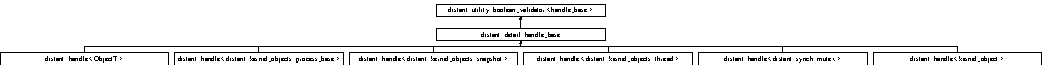
\includegraphics[height=0.840841cm]{classdistant_1_1detail_1_1handle__base}
\end{center}
\end{figure}
\subsection*{Public Types}
\begin{DoxyCompactItemize}
\item 
\mbox{\Hypertarget{classdistant_1_1detail_1_1handle__base_a5a10c6b2cfee1bcb626aead0a443561b}\label{classdistant_1_1detail_1_1handle__base_a5a10c6b2cfee1bcb626aead0a443561b}} 
using {\bfseries native\+\_\+type} = boost\+::winapi\+::\+H\+A\+N\+D\+L\+E\+\_\+
\item 
\mbox{\Hypertarget{classdistant_1_1detail_1_1handle__base_ad1b2c8670613be87fd9ca3f36222c406}\label{classdistant_1_1detail_1_1handle__base_ad1b2c8670613be87fd9ca3f36222c406}} 
using {\bfseries flag\+\_\+type} = access\+\_\+rights\+::handle
\end{DoxyCompactItemize}
\subsection*{Public Member Functions}
\begin{DoxyCompactItemize}
\item 
constexpr \mbox{\hyperlink{classdistant_1_1detail_1_1handle__base_a9f2003ece2e3183973e4fc9d7e6c99a7}{handle\+\_\+base}} (native\+\_\+type h, flag\+\_\+type \mbox{\hyperlink{classdistant_1_1detail_1_1handle__base_adc97dc91543d76d0b89f43fee5f5f26b}{flags}}=flag\+\_\+type\+::inherit, bool \mbox{\hyperlink{classdistant_1_1detail_1_1handle__base_abd5ad44b32fda79418c5faada682336a}{closed}}=false) noexcept
\item 
constexpr \mbox{\hyperlink{classdistant_1_1detail_1_1handle__base_a1a7acece6f6efdf438c2e5092451c8ec}{handle\+\_\+base}} (nullptr\+\_\+t h) noexcept
\item 
constexpr \mbox{\hyperlink{classdistant_1_1detail_1_1handle__base_aab5ad3c3cd411c27b87da8187ea51447}{handle\+\_\+base}} () noexcept
\item 
\mbox{\Hypertarget{classdistant_1_1detail_1_1handle__base_a7afbb166fe281e513aa0933a49eca638}\label{classdistant_1_1detail_1_1handle__base_a7afbb166fe281e513aa0933a49eca638}} 
\mbox{\hyperlink{classdistant_1_1detail_1_1handle__base_a7afbb166fe281e513aa0933a49eca638}{handle\+\_\+base}} (\mbox{\hyperlink{classdistant_1_1detail_1_1handle__base}{handle\+\_\+base}} \&\&) noexcept
\begin{DoxyCompactList}\small\item\em Move copyable. \end{DoxyCompactList}\item 
\mbox{\Hypertarget{classdistant_1_1detail_1_1handle__base_a2890bf2bab82df625da8a945e9be72df}\label{classdistant_1_1detail_1_1handle__base_a2890bf2bab82df625da8a945e9be72df}} 
\mbox{\hyperlink{classdistant_1_1detail_1_1handle__base}{handle\+\_\+base}} \& \mbox{\hyperlink{classdistant_1_1detail_1_1handle__base_a2890bf2bab82df625da8a945e9be72df}{operator=}} (\mbox{\hyperlink{classdistant_1_1detail_1_1handle__base}{handle\+\_\+base}} \&\&) noexcept
\begin{DoxyCompactList}\small\item\em Move assignable. \end{DoxyCompactList}\item 
\mbox{\Hypertarget{classdistant_1_1detail_1_1handle__base_ab7edeab674b5dee8f330ea8b210f4e01}\label{classdistant_1_1detail_1_1handle__base_ab7edeab674b5dee8f330ea8b210f4e01}} 
{\bfseries handle\+\_\+base} (const \mbox{\hyperlink{classdistant_1_1detail_1_1handle__base}{handle\+\_\+base}} \&)=delete
\item 
\mbox{\Hypertarget{classdistant_1_1detail_1_1handle__base_ac1e69f9ae94a849c04a4d25a684bb6f2}\label{classdistant_1_1detail_1_1handle__base_ac1e69f9ae94a849c04a4d25a684bb6f2}} 
\mbox{\hyperlink{classdistant_1_1detail_1_1handle__base}{handle\+\_\+base}} \& {\bfseries operator=} (const \mbox{\hyperlink{classdistant_1_1detail_1_1handle__base}{handle\+\_\+base}} \&)=delete
\item 
\mbox{\hyperlink{classdistant_1_1detail_1_1handle__base_aca25c1c62b12456c616ff3e010c61a8d}{$\sim$handle\+\_\+base}} () noexcept
\item 
bool \mbox{\hyperlink{classdistant_1_1detail_1_1handle__base_aa138b2e6e919a0199225403558e1b63d}{valid}} () const noexcept
\item 
bool \mbox{\hyperlink{classdistant_1_1detail_1_1handle__base_a6474b8752ffa2a3f3c75586be2fcf6b9}{close\+\_\+protected}} () const noexcept
\item 
bool \mbox{\hyperlink{classdistant_1_1detail_1_1handle__base_abd5ad44b32fda79418c5faada682336a}{closed}} () const noexcept
\item 
\mbox{\Hypertarget{classdistant_1_1detail_1_1handle__base_a761be454d0d8de053378d561abfb5afd}\label{classdistant_1_1detail_1_1handle__base_a761be454d0d8de053378d561abfb5afd}} 
bool \mbox{\hyperlink{classdistant_1_1detail_1_1handle__base_a761be454d0d8de053378d561abfb5afd}{close}} () noexcept
\begin{DoxyCompactList}\small\item\em Close the handle, if it is valid and its closure wasn\textquotesingle{}t observed. \end{DoxyCompactList}\item 
native\+\_\+type \mbox{\hyperlink{classdistant_1_1detail_1_1handle__base_a3207e125c17f2ebb59cab614083f782b}{native\+\_\+handle}} () const noexcept
\end{DoxyCompactItemize}
\subsection*{Protected Member Functions}
\begin{DoxyCompactItemize}
\item 
\mbox{\Hypertarget{classdistant_1_1detail_1_1handle__base_a6c93e0715a2cd1d29f65290b37d31504}\label{classdistant_1_1detail_1_1handle__base_a6c93e0715a2cd1d29f65290b37d31504}} 
void \mbox{\hyperlink{classdistant_1_1detail_1_1handle__base_a6c93e0715a2cd1d29f65290b37d31504}{invalidate}} () noexcept
\begin{DoxyCompactList}\small\item\em Numerically invalidate and close protect our handle. \end{DoxyCompactList}\item 
\mbox{\Hypertarget{classdistant_1_1detail_1_1handle__base_a8c70a0ccd10860c774b54d8656cbb910}\label{classdistant_1_1detail_1_1handle__base_a8c70a0ccd10860c774b54d8656cbb910}} 
void \mbox{\hyperlink{classdistant_1_1detail_1_1handle__base_a8c70a0ccd10860c774b54d8656cbb910}{protect}} () noexcept
\begin{DoxyCompactList}\small\item\em Protect the handle from being closed. \end{DoxyCompactList}\item 
flag\+\_\+type \mbox{\hyperlink{classdistant_1_1detail_1_1handle__base_adc97dc91543d76d0b89f43fee5f5f26b}{flags}} () const noexcept
\end{DoxyCompactItemize}
\subsection*{Protected Attributes}
\begin{DoxyCompactItemize}
\item 
\mbox{\Hypertarget{classdistant_1_1detail_1_1handle__base_ad46610dae2b7f1b3e0e2ab6bb8ef6b2e}\label{classdistant_1_1detail_1_1handle__base_ad46610dae2b7f1b3e0e2ab6bb8ef6b2e}} 
native\+\_\+type \mbox{\hyperlink{classdistant_1_1detail_1_1handle__base_ad46610dae2b7f1b3e0e2ab6bb8ef6b2e}{native\+\_\+handle\+\_\+}}
\begin{DoxyCompactList}\small\item\em native H\+A\+N\+D\+LE value \end{DoxyCompactList}\item 
\mbox{\Hypertarget{classdistant_1_1detail_1_1handle__base_af55692a0434e08d17849e92ad86c420d}\label{classdistant_1_1detail_1_1handle__base_af55692a0434e08d17849e92ad86c420d}} 
std\+::bitset$<$ 3 $>$ \mbox{\hyperlink{classdistant_1_1detail_1_1handle__base_af55692a0434e08d17849e92ad86c420d}{flags\+\_\+}}
\begin{DoxyCompactList}\small\item\em Switch to check if closure was observed. \end{DoxyCompactList}\end{DoxyCompactItemize}
\subsection*{Friends}
\begin{DoxyCompactItemize}
\item 
\mbox{\Hypertarget{classdistant_1_1detail_1_1handle__base_ae79375b4f4c33db8b147562e2ae3ef5d}\label{classdistant_1_1detail_1_1handle__base_ae79375b4f4c33db8b147562e2ae3ef5d}} 
constexpr bool {\bfseries operator==} (const \mbox{\hyperlink{classdistant_1_1detail_1_1handle__base}{handle\+\_\+base}} \&, const \mbox{\hyperlink{classdistant_1_1detail_1_1handle__base}{handle\+\_\+base}} \&) noexcept
\item 
\mbox{\Hypertarget{classdistant_1_1detail_1_1handle__base_a5d3970f4614aa751704be5d8749066e2}\label{classdistant_1_1detail_1_1handle__base_a5d3970f4614aa751704be5d8749066e2}} 
constexpr bool {\bfseries operator!=} (const \mbox{\hyperlink{classdistant_1_1detail_1_1handle__base}{handle\+\_\+base}} \&, const \mbox{\hyperlink{classdistant_1_1detail_1_1handle__base}{handle\+\_\+base}} \&) noexcept
\end{DoxyCompactItemize}


\subsection{Constructor \& Destructor Documentation}
\mbox{\Hypertarget{classdistant_1_1detail_1_1handle__base_a9f2003ece2e3183973e4fc9d7e6c99a7}\label{classdistant_1_1detail_1_1handle__base_a9f2003ece2e3183973e4fc9d7e6c99a7}} 
\index{distant\+::detail\+::handle\+\_\+base@{distant\+::detail\+::handle\+\_\+base}!handle\+\_\+base@{handle\+\_\+base}}
\index{handle\+\_\+base@{handle\+\_\+base}!distant\+::detail\+::handle\+\_\+base@{distant\+::detail\+::handle\+\_\+base}}
\subsubsection{\texorpdfstring{handle\+\_\+base()}{handle\_base()}\hspace{0.1cm}{\footnotesize\ttfamily [1/3]}}
{\footnotesize\ttfamily constexpr distant\+::detail\+::handle\+\_\+base\+::handle\+\_\+base (\begin{DoxyParamCaption}\item[{native\+\_\+type}]{h,  }\item[{flag\+\_\+type}]{flags = {\ttfamily flag\+\_\+type\+:\+:inherit},  }\item[{bool}]{closed = {\ttfamily false} }\end{DoxyParamCaption})\hspace{0.3cm}{\ttfamily [inline]}, {\ttfamily [explicit]}, {\ttfamily [noexcept]}}

Construct using native handle. 
\begin{DoxyParams}{Parameters}
{\em h} & the native handle value \\
\hline
{\em flags} & handle flags \\
\hline
\end{DoxyParams}
\mbox{\Hypertarget{classdistant_1_1detail_1_1handle__base_a1a7acece6f6efdf438c2e5092451c8ec}\label{classdistant_1_1detail_1_1handle__base_a1a7acece6f6efdf438c2e5092451c8ec}} 
\index{distant\+::detail\+::handle\+\_\+base@{distant\+::detail\+::handle\+\_\+base}!handle\+\_\+base@{handle\+\_\+base}}
\index{handle\+\_\+base@{handle\+\_\+base}!distant\+::detail\+::handle\+\_\+base@{distant\+::detail\+::handle\+\_\+base}}
\subsubsection{\texorpdfstring{handle\+\_\+base()}{handle\_base()}\hspace{0.1cm}{\footnotesize\ttfamily [2/3]}}
{\footnotesize\ttfamily constexpr distant\+::detail\+::handle\+\_\+base\+::handle\+\_\+base (\begin{DoxyParamCaption}\item[{nullptr\+\_\+t}]{h }\end{DoxyParamCaption})\hspace{0.3cm}{\ttfamily [inline]}, {\ttfamily [noexcept]}}

Construct an invalid handle. This allows handles to be comparable with nullptr. 
\begin{DoxyParams}{Parameters}
{\em h} & the nullptr. \\
\hline
\end{DoxyParams}
\mbox{\Hypertarget{classdistant_1_1detail_1_1handle__base_aab5ad3c3cd411c27b87da8187ea51447}\label{classdistant_1_1detail_1_1handle__base_aab5ad3c3cd411c27b87da8187ea51447}} 
\index{distant\+::detail\+::handle\+\_\+base@{distant\+::detail\+::handle\+\_\+base}!handle\+\_\+base@{handle\+\_\+base}}
\index{handle\+\_\+base@{handle\+\_\+base}!distant\+::detail\+::handle\+\_\+base@{distant\+::detail\+::handle\+\_\+base}}
\subsubsection{\texorpdfstring{handle\+\_\+base()}{handle\_base()}\hspace{0.1cm}{\footnotesize\ttfamily [3/3]}}
{\footnotesize\ttfamily constexpr distant\+::detail\+::handle\+\_\+base\+::handle\+\_\+base (\begin{DoxyParamCaption}{ }\end{DoxyParamCaption})\hspace{0.3cm}{\ttfamily [inline]}, {\ttfamily [noexcept]}}

Construct invalid handle. This calls the nullptr constructor. \mbox{\Hypertarget{classdistant_1_1detail_1_1handle__base_aca25c1c62b12456c616ff3e010c61a8d}\label{classdistant_1_1detail_1_1handle__base_aca25c1c62b12456c616ff3e010c61a8d}} 
\index{distant\+::detail\+::handle\+\_\+base@{distant\+::detail\+::handle\+\_\+base}!````~handle\+\_\+base@{$\sim$handle\+\_\+base}}
\index{````~handle\+\_\+base@{$\sim$handle\+\_\+base}!distant\+::detail\+::handle\+\_\+base@{distant\+::detail\+::handle\+\_\+base}}
\subsubsection{\texorpdfstring{$\sim$handle\+\_\+base()}{~handle\_base()}}
{\footnotesize\ttfamily distant\+::detail\+::handle\+\_\+base\+::$\sim$handle\+\_\+base (\begin{DoxyParamCaption}{ }\end{DoxyParamCaption})\hspace{0.3cm}{\ttfamily [inline]}, {\ttfamily [noexcept]}}

Close handle to windows object. Handle must be weakly valid in order to close the handle. 

\subsection{Member Function Documentation}
\mbox{\Hypertarget{classdistant_1_1detail_1_1handle__base_a6474b8752ffa2a3f3c75586be2fcf6b9}\label{classdistant_1_1detail_1_1handle__base_a6474b8752ffa2a3f3c75586be2fcf6b9}} 
\index{distant\+::detail\+::handle\+\_\+base@{distant\+::detail\+::handle\+\_\+base}!close\+\_\+protected@{close\+\_\+protected}}
\index{close\+\_\+protected@{close\+\_\+protected}!distant\+::detail\+::handle\+\_\+base@{distant\+::detail\+::handle\+\_\+base}}
\subsubsection{\texorpdfstring{close\+\_\+protected()}{close\_protected()}}
{\footnotesize\ttfamily bool distant\+::detail\+::handle\+\_\+base\+::close\+\_\+protected (\begin{DoxyParamCaption}{ }\end{DoxyParamCaption}) const\hspace{0.3cm}{\ttfamily [inline]}, {\ttfamily [noexcept]}}

Check if the handle is close protected \begin{DoxyReturn}{Returns}
true if the handle cannot be closed, false otherwise 
\end{DoxyReturn}
\mbox{\Hypertarget{classdistant_1_1detail_1_1handle__base_abd5ad44b32fda79418c5faada682336a}\label{classdistant_1_1detail_1_1handle__base_abd5ad44b32fda79418c5faada682336a}} 
\index{distant\+::detail\+::handle\+\_\+base@{distant\+::detail\+::handle\+\_\+base}!closed@{closed}}
\index{closed@{closed}!distant\+::detail\+::handle\+\_\+base@{distant\+::detail\+::handle\+\_\+base}}
\subsubsection{\texorpdfstring{closed()}{closed()}}
{\footnotesize\ttfamily bool distant\+::detail\+::handle\+\_\+base\+::closed (\begin{DoxyParamCaption}{ }\end{DoxyParamCaption}) const\hspace{0.3cm}{\ttfamily [inline]}, {\ttfamily [noexcept]}}

Check if handle\textquotesingle{}s closure has been observed \begin{DoxyReturn}{Returns}
true if the handle\textquotesingle{}s closure was observed, and false otherwise 
\end{DoxyReturn}
\mbox{\Hypertarget{classdistant_1_1detail_1_1handle__base_adc97dc91543d76d0b89f43fee5f5f26b}\label{classdistant_1_1detail_1_1handle__base_adc97dc91543d76d0b89f43fee5f5f26b}} 
\index{distant\+::detail\+::handle\+\_\+base@{distant\+::detail\+::handle\+\_\+base}!flags@{flags}}
\index{flags@{flags}!distant\+::detail\+::handle\+\_\+base@{distant\+::detail\+::handle\+\_\+base}}
\subsubsection{\texorpdfstring{flags()}{flags()}}
{\footnotesize\ttfamily handle\+\_\+base\+::flag\+\_\+type distant\+::detail\+::handle\+\_\+base\+::flags (\begin{DoxyParamCaption}{ }\end{DoxyParamCaption}) const\hspace{0.3cm}{\ttfamily [inline]}, {\ttfamily [protected]}, {\ttfamily [noexcept]}}

Get the handle\textquotesingle{}s flag type \begin{DoxyReturn}{Returns}
distant\+::access\+\_\+rights\+::handle flag type 
\end{DoxyReturn}
\mbox{\Hypertarget{classdistant_1_1detail_1_1handle__base_a3207e125c17f2ebb59cab614083f782b}\label{classdistant_1_1detail_1_1handle__base_a3207e125c17f2ebb59cab614083f782b}} 
\index{distant\+::detail\+::handle\+\_\+base@{distant\+::detail\+::handle\+\_\+base}!native\+\_\+handle@{native\+\_\+handle}}
\index{native\+\_\+handle@{native\+\_\+handle}!distant\+::detail\+::handle\+\_\+base@{distant\+::detail\+::handle\+\_\+base}}
\subsubsection{\texorpdfstring{native\+\_\+handle()}{native\_handle()}}
{\footnotesize\ttfamily handle\+\_\+base\+::native\+\_\+type distant\+::detail\+::handle\+\_\+base\+::native\+\_\+handle (\begin{DoxyParamCaption}{ }\end{DoxyParamCaption}) const\hspace{0.3cm}{\ttfamily [inline]}, {\ttfamily [noexcept]}}

Get the value of the native handle \begin{DoxyReturn}{Returns}
value of the native handle 
\end{DoxyReturn}
\mbox{\Hypertarget{classdistant_1_1detail_1_1handle__base_aa138b2e6e919a0199225403558e1b63d}\label{classdistant_1_1detail_1_1handle__base_aa138b2e6e919a0199225403558e1b63d}} 
\index{distant\+::detail\+::handle\+\_\+base@{distant\+::detail\+::handle\+\_\+base}!valid@{valid}}
\index{valid@{valid}!distant\+::detail\+::handle\+\_\+base@{distant\+::detail\+::handle\+\_\+base}}
\subsubsection{\texorpdfstring{valid()}{valid()}}
{\footnotesize\ttfamily bool distant\+::detail\+::handle\+\_\+base\+::valid (\begin{DoxyParamCaption}{ }\end{DoxyParamCaption}) const\hspace{0.3cm}{\ttfamily [inline]}, {\ttfamily [noexcept]}}

Checks the if the native handle is valid \begin{DoxyReturn}{Returns}
true if the native\+\_\+handle is not N\+U\+LL, and false otherwise 
\end{DoxyReturn}


The documentation for this class was generated from the following files\+:\begin{DoxyCompactItemize}
\item 
C\+:/\+Users/dinne/source/repos/distant dev/distant dev/include/distant/detail/handle\+\_\+base.\+hpp\item 
C\+:/\+Users/dinne/source/repos/distant dev/distant dev/include/distant/impl/handle\+\_\+base.\+hxx\end{DoxyCompactItemize}

\hypertarget{structdistant_1_1kernel__objects_1_1detail_1_1has__token__access}{}\section{distant\+:\+:kernel\+\_\+objects\+:\+:detail\+:\+:has\+\_\+token\+\_\+access$<$ typename $>$ Struct Template Reference}
\label{structdistant_1_1kernel__objects_1_1detail_1_1has__token__access}\index{distant\+::kernel\+\_\+objects\+::detail\+::has\+\_\+token\+\_\+access$<$ typename $>$@{distant\+::kernel\+\_\+objects\+::detail\+::has\+\_\+token\+\_\+access$<$ typename $>$}}


The documentation for this struct was generated from the following file\+:\begin{DoxyCompactItemize}
\item 
C\+:/\+Users/dinne/source/repos/distant dev/distant dev/include/distant/kernel\+\_\+objects/type\+\_\+traits.\+hpp\end{DoxyCompactItemize}

\hypertarget{structdistant_1_1kernel__objects_1_1detail_1_1has__token__access_3_01process_3_01_a_01_4_01_4}{}\section{distant\+:\+:kernel\+\_\+objects\+:\+:detail\+:\+:has\+\_\+token\+\_\+access$<$ process$<$ A $>$ $>$ Struct Template Reference}
\label{structdistant_1_1kernel__objects_1_1detail_1_1has__token__access_3_01process_3_01_a_01_4_01_4}\index{distant\+::kernel\+\_\+objects\+::detail\+::has\+\_\+token\+\_\+access$<$ process$<$ A $>$ $>$@{distant\+::kernel\+\_\+objects\+::detail\+::has\+\_\+token\+\_\+access$<$ process$<$ A $>$ $>$}}
\subsection*{Static Public Attributes}
\begin{DoxyCompactItemize}
\item 
\mbox{\Hypertarget{structdistant_1_1kernel__objects_1_1detail_1_1has__token__access_3_01process_3_01_a_01_4_01_4_a8e5a5e4e0c4e6b3d2786f89ea293812b}\label{structdistant_1_1kernel__objects_1_1detail_1_1has__token__access_3_01process_3_01_a_01_4_01_4_a8e5a5e4e0c4e6b3d2786f89ea293812b}} 
static constexpr bool {\bfseries value} = check\+\_\+permission(A, process\+\_\+rights\+::query\+\_\+information)
\end{DoxyCompactItemize}


The documentation for this struct was generated from the following file\+:\begin{DoxyCompactItemize}
\item 
C\+:/\+Users/dinne/source/repos/distant dev/distant dev/include/distant/kernel\+\_\+objects/type\+\_\+traits.\+hpp\end{DoxyCompactItemize}

\hypertarget{structdistant_1_1utility_1_1meta_1_1hash}{}\section{distant\+:\+:utility\+:\+:meta\+:\+:hash$<$ T $>$ Struct Template Reference}
\label{structdistant_1_1utility_1_1meta_1_1hash}\index{distant\+::utility\+::meta\+::hash$<$ T $>$@{distant\+::utility\+::meta\+::hash$<$ T $>$}}
\subsection*{Public Member Functions}
\begin{DoxyCompactItemize}
\item 
\mbox{\Hypertarget{structdistant_1_1utility_1_1meta_1_1hash_a471097e58bb0da13db4c6a9f3f79f208}\label{structdistant_1_1utility_1_1meta_1_1hash_a471097e58bb0da13db4c6a9f3f79f208}} 
constexpr std\+::size\+\_\+t {\bfseries operator()} (const T \&key) const noexcept
\end{DoxyCompactItemize}


The documentation for this struct was generated from the following files\+:\begin{DoxyCompactItemize}
\item 
C\+:/\+Users/dinne/source/repos/distant dev/distant dev/include/distant/utility/meta/hash.\+hpp\item 
C\+:/\+Users/dinne/source/repos/distant dev/distant dev/include/distant/utility/meta/impl/hash.\+hxx\end{DoxyCompactItemize}

\hypertarget{structstd_1_1hash_3_01distant_1_1memory_1_1address_3_01_a_01_4_01_4}{}\section{std\+:\+:hash$<$ distant\+:\+:memory\+:\+:address$<$ A $>$ $>$ Struct Template Reference}
\label{structstd_1_1hash_3_01distant_1_1memory_1_1address_3_01_a_01_4_01_4}\index{std\+::hash$<$ distant\+::memory\+::address$<$ A $>$ $>$@{std\+::hash$<$ distant\+::memory\+::address$<$ A $>$ $>$}}
\subsection*{Public Types}
\begin{DoxyCompactItemize}
\item 
\mbox{\Hypertarget{structstd_1_1hash_3_01distant_1_1memory_1_1address_3_01_a_01_4_01_4_acc28636c44fb1d5eeddb61942f3bdbcf}\label{structstd_1_1hash_3_01distant_1_1memory_1_1address_3_01_a_01_4_01_4_acc28636c44fb1d5eeddb61942f3bdbcf}} 
using {\bfseries argument\+\_\+type} = \mbox{\hyperlink{classdistant_1_1memory_1_1address}{distant\+::memory\+::address}}$<$ A $>$
\item 
\mbox{\Hypertarget{structstd_1_1hash_3_01distant_1_1memory_1_1address_3_01_a_01_4_01_4_a8dee9ef0ee1f2ac63756bf24b180ed7e}\label{structstd_1_1hash_3_01distant_1_1memory_1_1address_3_01_a_01_4_01_4_a8dee9ef0ee1f2ac63756bf24b180ed7e}} 
using {\bfseries result\+\_\+type} = std\+::size\+\_\+t
\end{DoxyCompactItemize}
\subsection*{Public Member Functions}
\begin{DoxyCompactItemize}
\item 
\mbox{\Hypertarget{structstd_1_1hash_3_01distant_1_1memory_1_1address_3_01_a_01_4_01_4_ae8e520d90f9d08b949333c2908a70118}\label{structstd_1_1hash_3_01distant_1_1memory_1_1address_3_01_a_01_4_01_4_ae8e520d90f9d08b949333c2908a70118}} 
result\+\_\+type {\bfseries operator()} (const \mbox{\hyperlink{classdistant_1_1memory_1_1address}{argument\+\_\+type}} \&address) const noexcept
\end{DoxyCompactItemize}


The documentation for this struct was generated from the following file\+:\begin{DoxyCompactItemize}
\item 
C\+:/\+Users/dinne/source/repos/distant dev/distant dev/include/distant/memory/impl/address.\+hxx\end{DoxyCompactItemize}

\hypertarget{classdistant_1_1synch_1_1wait_1_1infinite}{}\section{distant\+:\+:synch\+:\+:wait\+:\+:infinite Class Reference}
\label{classdistant_1_1synch_1_1wait_1_1infinite}\index{distant\+::synch\+::wait\+::infinite@{distant\+::synch\+::wait\+::infinite}}
Inheritance diagram for distant\+:\+:synch\+:\+:wait\+:\+:infinite\+:\begin{figure}[H]
\begin{center}
\leavevmode
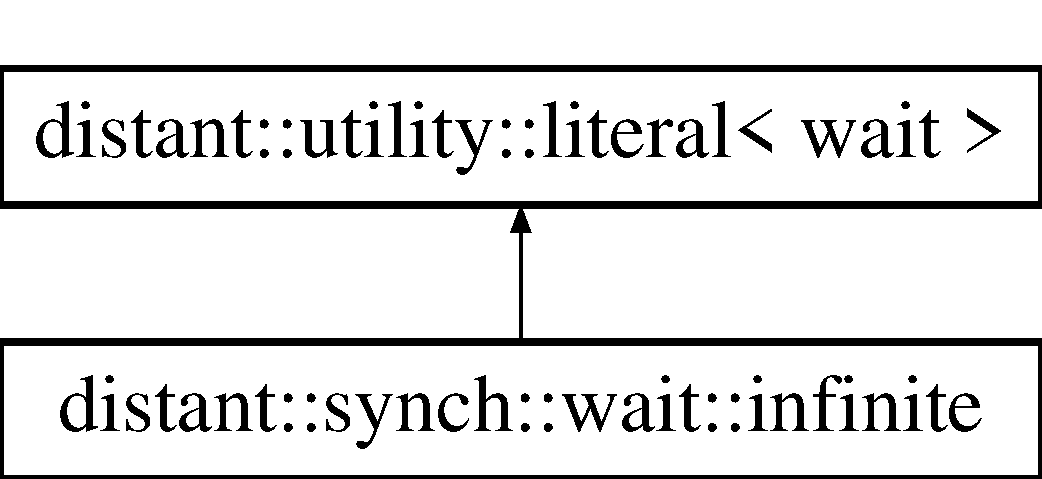
\includegraphics[height=2.000000cm]{classdistant_1_1synch_1_1wait_1_1infinite}
\end{center}
\end{figure}
\subsection*{Additional Inherited Members}


The documentation for this class was generated from the following file\+:\begin{DoxyCompactItemize}
\item 
C\+:/\+Users/dinne/source/repos/distant dev/distant dev/include/distant/synch/wait.\+hpp\end{DoxyCompactItemize}

\hypertarget{structdistant_1_1is__kernel__object}{}\section{distant\+:\+:is\+\_\+kernel\+\_\+object$<$ T $>$ Struct Template Reference}
\label{structdistant_1_1is__kernel__object}\index{distant\+::is\+\_\+kernel\+\_\+object$<$ T $>$@{distant\+::is\+\_\+kernel\+\_\+object$<$ T $>$}}
\subsection*{Public Types}
\begin{DoxyCompactItemize}
\item 
\mbox{\Hypertarget{structdistant_1_1is__kernel__object_a6d8a379fa5475e8f974817395ebe3dc7}\label{structdistant_1_1is__kernel__object_a6d8a379fa5475e8f974817395ebe3dc7}} 
using {\bfseries result} = std\+::conditional\+\_\+t$<$ std\+::is\+\_\+convertible$<$ T, \mbox{\hyperlink{classdistant_1_1kernel__objects_1_1kernel__object}{kernel\+\_\+objects\+::kernel\+\_\+object}} $>$\+::value, std\+::true\+\_\+type, std\+::false\+\_\+type $>$
\end{DoxyCompactItemize}
\subsection*{Static Public Attributes}
\begin{DoxyCompactItemize}
\item 
\mbox{\Hypertarget{structdistant_1_1is__kernel__object_a1addaa93158a790ca5bda1532b4f6c8a}\label{structdistant_1_1is__kernel__object_a1addaa93158a790ca5bda1532b4f6c8a}} 
static constexpr bool {\bfseries value} = result\+::value
\end{DoxyCompactItemize}


The documentation for this struct was generated from the following file\+:\begin{DoxyCompactItemize}
\item 
C\+:/\+Users/dinne/source/repos/distant dev/distant dev/include/distant/type\+\_\+traits.\+hpp\end{DoxyCompactItemize}

\hypertarget{structstd_1_1iterator__traits_3_01distant_1_1memory_1_1virtual__ptr_3_01_element_00_01_address_t_01_4_01_4}{}\section{std\+:\+:iterator\+\_\+traits$<$ distant\+:\+:memory\+:\+:virtual\+\_\+ptr$<$ Element, AddressT $>$ $>$ Struct Template Reference}
\label{structstd_1_1iterator__traits_3_01distant_1_1memory_1_1virtual__ptr_3_01_element_00_01_address_t_01_4_01_4}\index{std\+::iterator\+\_\+traits$<$ distant\+::memory\+::virtual\+\_\+ptr$<$ Element, Address\+T $>$ $>$@{std\+::iterator\+\_\+traits$<$ distant\+::memory\+::virtual\+\_\+ptr$<$ Element, Address\+T $>$ $>$}}
\subsection*{Public Types}
\begin{DoxyCompactItemize}
\item 
\mbox{\Hypertarget{structstd_1_1iterator__traits_3_01distant_1_1memory_1_1virtual__ptr_3_01_element_00_01_address_t_01_4_01_4_a0574fcbe68898aabe830c86f39a2679d}\label{structstd_1_1iterator__traits_3_01distant_1_1memory_1_1virtual__ptr_3_01_element_00_01_address_t_01_4_01_4_a0574fcbe68898aabe830c86f39a2679d}} 
using {\bfseries difference\+\_\+type} = typename pointer\+\_\+traits$<$ \mbox{\hyperlink{classdistant_1_1memory_1_1virtual__ptr}{vptr\+\_\+t}} $>$\+::difference\+\_\+type
\item 
\mbox{\Hypertarget{structstd_1_1iterator__traits_3_01distant_1_1memory_1_1virtual__ptr_3_01_element_00_01_address_t_01_4_01_4_af3dc39ab8e8fcda98f26a58b6eef64a0}\label{structstd_1_1iterator__traits_3_01distant_1_1memory_1_1virtual__ptr_3_01_element_00_01_address_t_01_4_01_4_af3dc39ab8e8fcda98f26a58b6eef64a0}} 
using {\bfseries pointer} = typename pointer\+\_\+traits$<$ \mbox{\hyperlink{classdistant_1_1memory_1_1virtual__ptr}{vptr\+\_\+t}} $>$\+::pointer
\item 
\mbox{\Hypertarget{structstd_1_1iterator__traits_3_01distant_1_1memory_1_1virtual__ptr_3_01_element_00_01_address_t_01_4_01_4_a97c5fe38887d6eabf3a75871c5e8d49c}\label{structstd_1_1iterator__traits_3_01distant_1_1memory_1_1virtual__ptr_3_01_element_00_01_address_t_01_4_01_4_a97c5fe38887d6eabf3a75871c5e8d49c}} 
using {\bfseries value\+\_\+type} = typename pointer\+\_\+traits$<$ \mbox{\hyperlink{classdistant_1_1memory_1_1virtual__ptr}{vptr\+\_\+t}} $>$\+::element\+\_\+type
\item 
\mbox{\Hypertarget{structstd_1_1iterator__traits_3_01distant_1_1memory_1_1virtual__ptr_3_01_element_00_01_address_t_01_4_01_4_a73730119926d04f012b91ab1cedec94e}\label{structstd_1_1iterator__traits_3_01distant_1_1memory_1_1virtual__ptr_3_01_element_00_01_address_t_01_4_01_4_a73730119926d04f012b91ab1cedec94e}} 
using {\bfseries reference} = \mbox{\hyperlink{classdistant_1_1memory_1_1virtual__reference}{distant\+::memory\+::virtual\+\_\+reference}}$<$ Element, AddressT $>$
\item 
\mbox{\Hypertarget{structstd_1_1iterator__traits_3_01distant_1_1memory_1_1virtual__ptr_3_01_element_00_01_address_t_01_4_01_4_a808047c9bf3da29e18c6e8717df8b14c}\label{structstd_1_1iterator__traits_3_01distant_1_1memory_1_1virtual__ptr_3_01_element_00_01_address_t_01_4_01_4_a808047c9bf3da29e18c6e8717df8b14c}} 
using {\bfseries iterator\+\_\+category} = std\+::random\+\_\+access\+\_\+iterator\+\_\+tag
\end{DoxyCompactItemize}


The documentation for this struct was generated from the following file\+:\begin{DoxyCompactItemize}
\item 
C\+:/\+Users/dinne/source/repos/distant dev/distant dev/include/distant/memory/virtual\+\_\+ptr.\+hpp\end{DoxyCompactItemize}

\hypertarget{classdistant_1_1kernel__objects_1_1kernel__object}{}\section{distant\+:\+:kernel\+\_\+objects\+:\+:kernel\+\_\+object Class Reference}
\label{classdistant_1_1kernel__objects_1_1kernel__object}\index{distant\+::kernel\+\_\+objects\+::kernel\+\_\+object@{distant\+::kernel\+\_\+objects\+::kernel\+\_\+object}}


Base class for kernel objects.  




{\ttfamily \#include $<$kernel\+\_\+object.\+hpp$>$}

Inheritance diagram for distant\+:\+:kernel\+\_\+objects\+:\+:kernel\+\_\+object\+:\begin{figure}[H]
\begin{center}
\leavevmode
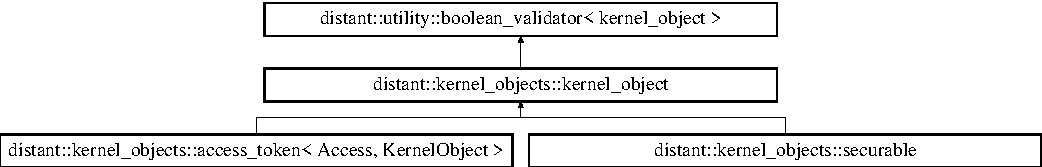
\includegraphics[height=2.234043cm]{classdistant_1_1kernel__objects_1_1kernel__object}
\end{center}
\end{figure}
\subsection*{Public Types}
\begin{DoxyCompactItemize}
\item 
\mbox{\Hypertarget{classdistant_1_1kernel__objects_1_1kernel__object_aa51e24680263a8b22bcf8b8ac77380a3}\label{classdistant_1_1kernel__objects_1_1kernel__object_aa51e24680263a8b22bcf8b8ac77380a3}} 
using {\bfseries handle\+\_\+type} = \mbox{\hyperlink{classdistant_1_1handle}{handle}}$<$ \mbox{\hyperlink{classdistant_1_1kernel__objects_1_1kernel__object}{kernel\+\_\+object}} $>$
\end{DoxyCompactItemize}
\subsection*{Public Member Functions}
\begin{DoxyCompactItemize}
\item 
\mbox{\Hypertarget{classdistant_1_1kernel__objects_1_1kernel__object_a460b6e2e735af256b6ef6c155c9bada7}\label{classdistant_1_1kernel__objects_1_1kernel__object_a460b6e2e735af256b6ef6c155c9bada7}} 
{\footnotesize template$<$typename Kernel\+Object , typename  = std\+::enable\+\_\+if\+\_\+t$<$std\+::is\+\_\+convertible$<$\+Kernel\+Object, kernel\+\_\+object$>$\+::value$>$$>$ }\\const \mbox{\hyperlink{classdistant_1_1handle}{distant\+::handle}}$<$ Kernel\+Object $>$ \& \mbox{\hyperlink{classdistant_1_1kernel__objects_1_1kernel__object_a460b6e2e735af256b6ef6c155c9bada7}{handle}} () const noexcept
\begin{DoxyCompactList}\small\item\em Bivariant type cast for kernel objects. \end{DoxyCompactList}\item 
const \mbox{\hyperlink{classdistant_1_1handle}{distant\+::handle}}$<$ \mbox{\hyperlink{classdistant_1_1kernel__objects_1_1kernel__object}{kernel\+\_\+object}} $>$ \& \mbox{\hyperlink{classdistant_1_1kernel__objects_1_1kernel__object_ad987412d770537d60500a007d7bc3d9e}{handle}} () const noexcept
\begin{DoxyCompactList}\small\item\em Get a handle to the \mbox{\hyperlink{classdistant_1_1kernel__objects_1_1kernel__object}{kernel\+\_\+object}}. \end{DoxyCompactList}\item 
virtual bool \mbox{\hyperlink{classdistant_1_1kernel__objects_1_1kernel__object_a07c26f8b2f2121367d9a71c64d3bf2c4}{valid}} () const noexcept
\begin{DoxyCompactList}\small\item\em Check if the \mbox{\hyperlink{classdistant_1_1kernel__objects_1_1kernel__object}{kernel\+\_\+object}} is valid. \end{DoxyCompactList}\item 
\mbox{\Hypertarget{classdistant_1_1kernel__objects_1_1kernel__object_a7288c3a2239ab03b1e24ba6970349723}\label{classdistant_1_1kernel__objects_1_1kernel__object_a7288c3a2239ab03b1e24ba6970349723}} 
virtual \mbox{\hyperlink{classdistant_1_1kernel__objects_1_1kernel__object_a7288c3a2239ab03b1e24ba6970349723}{$\sim$kernel\+\_\+object}} ()=default
\begin{DoxyCompactList}\small\item\em Declare the destructor virtual to prevent slicing. \end{DoxyCompactList}\item 
\mbox{\Hypertarget{classdistant_1_1kernel__objects_1_1kernel__object_a4c301e6f3c9df1ad43f803907fc20150}\label{classdistant_1_1kernel__objects_1_1kernel__object_a4c301e6f3c9df1ad43f803907fc20150}} 
\mbox{\hyperlink{classdistant_1_1kernel__objects_1_1kernel__object_a4c301e6f3c9df1ad43f803907fc20150}{kernel\+\_\+object}} () noexcept
\begin{DoxyCompactList}\small\item\em Invalid handle default constructor. \end{DoxyCompactList}\item 
\mbox{\Hypertarget{classdistant_1_1kernel__objects_1_1kernel__object_a7a192cbe9a25c132506a39ea9f3af93a}\label{classdistant_1_1kernel__objects_1_1kernel__object_a7a192cbe9a25c132506a39ea9f3af93a}} 
{\bfseries kernel\+\_\+object} (\mbox{\hyperlink{classdistant_1_1handle}{handle\+\_\+type}} \&\&\mbox{\hyperlink{classdistant_1_1handle}{handle}}) noexcept
\item 
\mbox{\Hypertarget{classdistant_1_1kernel__objects_1_1kernel__object_a2e6dfdf7488d70a99b3066b3568c1c23}\label{classdistant_1_1kernel__objects_1_1kernel__object_a2e6dfdf7488d70a99b3066b3568c1c23}} 
\mbox{\hyperlink{classdistant_1_1kernel__objects_1_1kernel__object_a2e6dfdf7488d70a99b3066b3568c1c23}{kernel\+\_\+object}} (\mbox{\hyperlink{classdistant_1_1kernel__objects_1_1kernel__object}{kernel\+\_\+object}} \&\&other) noexcept=default
\begin{DoxyCompactList}\small\item\em Move constructible. \end{DoxyCompactList}\item 
\mbox{\Hypertarget{classdistant_1_1kernel__objects_1_1kernel__object_ae6ecda6a08c6cd9a5e9ac6740d549644}\label{classdistant_1_1kernel__objects_1_1kernel__object_ae6ecda6a08c6cd9a5e9ac6740d549644}} 
\mbox{\hyperlink{classdistant_1_1kernel__objects_1_1kernel__object}{kernel\+\_\+object}} \& \mbox{\hyperlink{classdistant_1_1kernel__objects_1_1kernel__object_ae6ecda6a08c6cd9a5e9ac6740d549644}{operator=}} (\mbox{\hyperlink{classdistant_1_1kernel__objects_1_1kernel__object}{kernel\+\_\+object}} \&\&other) noexcept=default
\begin{DoxyCompactList}\small\item\em Move assignable. \end{DoxyCompactList}\end{DoxyCompactItemize}
\subsection*{Protected Attributes}
\begin{DoxyCompactItemize}
\item 
\mbox{\Hypertarget{classdistant_1_1kernel__objects_1_1kernel__object_ad1107811388709bb8c59eebc64101b31}\label{classdistant_1_1kernel__objects_1_1kernel__object_ad1107811388709bb8c59eebc64101b31}} 
\mbox{\hyperlink{classdistant_1_1handle}{handle\+\_\+type}} {\bfseries handle\+\_\+}
\end{DoxyCompactItemize}


\subsection{Detailed Description}
Base class for kernel objects. 

\subsection{Member Function Documentation}
\mbox{\Hypertarget{classdistant_1_1kernel__objects_1_1kernel__object_ad987412d770537d60500a007d7bc3d9e}\label{classdistant_1_1kernel__objects_1_1kernel__object_ad987412d770537d60500a007d7bc3d9e}} 
\index{distant\+::kernel\+\_\+objects\+::kernel\+\_\+object@{distant\+::kernel\+\_\+objects\+::kernel\+\_\+object}!handle@{handle}}
\index{handle@{handle}!distant\+::kernel\+\_\+objects\+::kernel\+\_\+object@{distant\+::kernel\+\_\+objects\+::kernel\+\_\+object}}
\subsubsection{\texorpdfstring{handle()}{handle()}}
{\footnotesize\ttfamily const \mbox{\hyperlink{classdistant_1_1handle}{distant\+::handle}}$<$ \mbox{\hyperlink{classdistant_1_1kernel__objects_1_1kernel__object}{kernel\+\_\+object}} $>$ \& distant\+::kernel\+\_\+objects\+::kernel\+\_\+object\+::handle (\begin{DoxyParamCaption}{ }\end{DoxyParamCaption}) const\hspace{0.3cm}{\ttfamily [inline]}, {\ttfamily [noexcept]}}



Get a handle to the \mbox{\hyperlink{classdistant_1_1kernel__objects_1_1kernel__object}{kernel\+\_\+object}}. 

\begin{DoxyReturn}{Returns}
a type-\/safe handle to the \mbox{\hyperlink{classdistant_1_1kernel__objects_1_1kernel__object}{kernel\+\_\+object}}. 
\end{DoxyReturn}
\mbox{\Hypertarget{classdistant_1_1kernel__objects_1_1kernel__object_a07c26f8b2f2121367d9a71c64d3bf2c4}\label{classdistant_1_1kernel__objects_1_1kernel__object_a07c26f8b2f2121367d9a71c64d3bf2c4}} 
\index{distant\+::kernel\+\_\+objects\+::kernel\+\_\+object@{distant\+::kernel\+\_\+objects\+::kernel\+\_\+object}!valid@{valid}}
\index{valid@{valid}!distant\+::kernel\+\_\+objects\+::kernel\+\_\+object@{distant\+::kernel\+\_\+objects\+::kernel\+\_\+object}}
\subsubsection{\texorpdfstring{valid()}{valid()}}
{\footnotesize\ttfamily bool distant\+::kernel\+\_\+objects\+::kernel\+\_\+object\+::valid (\begin{DoxyParamCaption}{ }\end{DoxyParamCaption}) const\hspace{0.3cm}{\ttfamily [inline]}, {\ttfamily [virtual]}, {\ttfamily [noexcept]}}



Check if the \mbox{\hyperlink{classdistant_1_1kernel__objects_1_1kernel__object}{kernel\+\_\+object}} is valid. 

\begin{DoxyReturn}{Returns}
true if the \mbox{\hyperlink{classdistant_1_1kernel__objects_1_1kernel__object}{kernel\+\_\+object}} is valid. 
\end{DoxyReturn}


The documentation for this class was generated from the following files\+:\begin{DoxyCompactItemize}
\item 
C\+:/\+Users/dinne/source/repos/distant dev/distant dev/include/distant/kernel\+\_\+objects/kernel\+\_\+object.\+hpp\item 
C\+:/\+Users/dinne/source/repos/distant dev/distant dev/include/distant/kernel\+\_\+objects/impl/kernel\+\_\+object.\+hxx\end{DoxyCompactItemize}

\hypertarget{structdistant_1_1kernel__object__traits}{}\section{distant\+:\+:kernel\+\_\+object\+\_\+traits$<$ T $>$ Struct Template Reference}
\label{structdistant_1_1kernel__object__traits}\index{distant\+::kernel\+\_\+object\+\_\+traits$<$ T $>$@{distant\+::kernel\+\_\+object\+\_\+traits$<$ T $>$}}


Contains kernel\+\_\+object traits.  




{\ttfamily \#include $<$type\+\_\+traits.\+hpp$>$}

\subsection*{Public Types}
\begin{DoxyCompactItemize}
\item 
\mbox{\Hypertarget{structdistant_1_1kernel__object__traits_a937d5543766e1377cba1a5cfa2033efc}\label{structdistant_1_1kernel__object__traits_a937d5543766e1377cba1a5cfa2033efc}} 
using {\bfseries handle\+\_\+type} = \mbox{\hyperlink{classdistant_1_1handle}{handle}}$<$ T $>$
\item 
\mbox{\Hypertarget{structdistant_1_1kernel__object__traits_a9effba9262500c321af99969236b72a6}\label{structdistant_1_1kernel__object__traits_a9effba9262500c321af99969236b72a6}} 
using {\bfseries native\+\_\+handle\+\_\+type} = void $\ast$
\item 
\mbox{\Hypertarget{structdistant_1_1kernel__object__traits_a5dba6e5dfc0831aea1e024edd4cfb7d3}\label{structdistant_1_1kernel__object__traits_a5dba6e5dfc0831aea1e024edd4cfb7d3}} 
using {\bfseries error\+\_\+type} = \mbox{\hyperlink{classdistant_1_1error_1_1windows__error__code}{error\+::windows\+\_\+error\+\_\+code}}
\item 
\mbox{\Hypertarget{structdistant_1_1kernel__object__traits_a7e9548e129037c9dfcd73c816019360e}\label{structdistant_1_1kernel__object__traits_a7e9548e129037c9dfcd73c816019360e}} 
using {\bfseries object\+\_\+type} = T
\end{DoxyCompactItemize}


\subsection{Detailed Description}
\subsubsection*{template$<$class T$>$\newline
struct distant\+::kernel\+\_\+object\+\_\+traits$<$ T $>$}

Contains kernel\+\_\+object traits. 

The documentation for this struct was generated from the following file\+:\begin{DoxyCompactItemize}
\item 
C\+:/\+Users/dinne/source/repos/distant dev/distant dev/include/distant/type\+\_\+traits.\+hpp\end{DoxyCompactItemize}

\hypertarget{classdistant_1_1utility_1_1literal}{}\section{distant\+:\+:utility\+:\+:literal$<$ LiteralT $>$ Class Template Reference}
\label{classdistant_1_1utility_1_1literal}\index{distant\+::utility\+::literal$<$ Literal\+T $>$@{distant\+::utility\+::literal$<$ Literal\+T $>$}}
\subsection*{Public Member Functions}
\begin{DoxyCompactItemize}
\item 
\mbox{\Hypertarget{classdistant_1_1utility_1_1literal_a71180d2699c72362c9210d261fc7210e}\label{classdistant_1_1utility_1_1literal_a71180d2699c72362c9210d261fc7210e}} 
void $\ast$ {\bfseries operator new} (std\+::size\+\_\+t)=delete
\item 
\mbox{\Hypertarget{classdistant_1_1utility_1_1literal_ad56dcf3bf89a82c6c9c7f6845a2fdcab}\label{classdistant_1_1utility_1_1literal_ad56dcf3bf89a82c6c9c7f6845a2fdcab}} 
void {\bfseries operator delete} (void $\ast$)=delete
\item 
\mbox{\Hypertarget{classdistant_1_1utility_1_1literal_a66fbff5d5fb0600a3ae661168af86ed5}\label{classdistant_1_1utility_1_1literal_a66fbff5d5fb0600a3ae661168af86ed5}} 
void {\bfseries operator\&} ()=delete
\item 
\mbox{\Hypertarget{classdistant_1_1utility_1_1literal_a42efe6ba50cd1acd57dbd1e50cf3d1e8}\label{classdistant_1_1utility_1_1literal_a42efe6ba50cd1acd57dbd1e50cf3d1e8}} 
void {\bfseries operator=} (const \mbox{\hyperlink{classdistant_1_1utility_1_1literal}{literal}} \&)=delete
\end{DoxyCompactItemize}


The documentation for this class was generated from the following file\+:\begin{DoxyCompactItemize}
\item 
C\+:/\+Users/dinne/source/repos/distant dev/distant dev/include/distant/utility/literal.\+hpp\end{DoxyCompactItemize}

\hypertarget{classdistant_1_1synch_1_1lock__guard}{}\section{distant\+:\+:synch\+:\+:lock\+\_\+guard$<$ Mutex $>$ Class Template Reference}
\label{classdistant_1_1synch_1_1lock__guard}\index{distant\+::synch\+::lock\+\_\+guard$<$ Mutex $>$@{distant\+::synch\+::lock\+\_\+guard$<$ Mutex $>$}}
\subsection*{Public Member Functions}
\begin{DoxyCompactItemize}
\item 
\mbox{\hyperlink{classdistant_1_1synch_1_1lock__guard_afe37b69ebfc05c1c97eb474cfdf9b4f1}{lock\+\_\+guard}} (Mutex \&\mbox{\hyperlink{classdistant_1_1synch_1_1mutex}{mutex}}, bool adopt\+\_\+mutex=false)
\begin{DoxyCompactList}\small\item\em Construct a guard that will attempt to lock the mutex, or will do nothing if the mutex is adopted. \end{DoxyCompactList}\item 
\mbox{\Hypertarget{classdistant_1_1synch_1_1lock__guard_a27c4df5411f53f7ba466abe100660dd3}\label{classdistant_1_1synch_1_1lock__guard_a27c4df5411f53f7ba466abe100660dd3}} 
\mbox{\hyperlink{classdistant_1_1synch_1_1lock__guard_a27c4df5411f53f7ba466abe100660dd3}{$\sim$lock\+\_\+guard}} () noexcept
\begin{DoxyCompactList}\small\item\em Unlock the mutex upon destruction of the guard. \end{DoxyCompactList}\item 
\mbox{\Hypertarget{classdistant_1_1synch_1_1lock__guard_aab05fca878249d4b4ba94b80653ffd59}\label{classdistant_1_1synch_1_1lock__guard_aab05fca878249d4b4ba94b80653ffd59}} 
{\bfseries lock\+\_\+guard} (const \mbox{\hyperlink{classdistant_1_1synch_1_1lock__guard}{lock\+\_\+guard}} \&)=delete
\item 
\mbox{\Hypertarget{classdistant_1_1synch_1_1lock__guard_aebcc75617792e91eb555f721f3d4e838}\label{classdistant_1_1synch_1_1lock__guard_aebcc75617792e91eb555f721f3d4e838}} 
\mbox{\hyperlink{classdistant_1_1synch_1_1lock__guard}{lock\+\_\+guard}} \& {\bfseries operator=} (const \mbox{\hyperlink{classdistant_1_1synch_1_1lock__guard}{lock\+\_\+guard}} \&)=delete
\end{DoxyCompactItemize}


\subsection{Constructor \& Destructor Documentation}
\mbox{\Hypertarget{classdistant_1_1synch_1_1lock__guard_afe37b69ebfc05c1c97eb474cfdf9b4f1}\label{classdistant_1_1synch_1_1lock__guard_afe37b69ebfc05c1c97eb474cfdf9b4f1}} 
\index{distant\+::synch\+::lock\+\_\+guard@{distant\+::synch\+::lock\+\_\+guard}!lock\+\_\+guard@{lock\+\_\+guard}}
\index{lock\+\_\+guard@{lock\+\_\+guard}!distant\+::synch\+::lock\+\_\+guard@{distant\+::synch\+::lock\+\_\+guard}}
\subsubsection{\texorpdfstring{lock\+\_\+guard()}{lock\_guard()}}
{\footnotesize\ttfamily template$<$typename Mutex $>$ \\
\mbox{\hyperlink{classdistant_1_1synch_1_1lock__guard}{distant\+::synch\+::lock\+\_\+guard}}$<$ Mutex $>$\+::\mbox{\hyperlink{classdistant_1_1synch_1_1lock__guard}{lock\+\_\+guard}} (\begin{DoxyParamCaption}\item[{Mutex \&}]{mutex,  }\item[{bool}]{adopt\+\_\+mutex = {\ttfamily false} }\end{DoxyParamCaption})}



Construct a guard that will attempt to lock the mutex, or will do nothing if the mutex is adopted. 


\begin{DoxyParams}{Parameters}
{\em mutex} & the mutex to guard. \\
\hline
{\em adopt\+\_\+mutex} & determines whether the mutex will be locked or not. \\
\hline
\end{DoxyParams}


The documentation for this class was generated from the following files\+:\begin{DoxyCompactItemize}
\item 
C\+:/\+Users/dinne/source/repos/distant dev/distant dev/include/distant/synch/fwd.\+hpp\item 
C\+:/\+Users/dinne/source/repos/distant dev/distant dev/include/distant/synch/mutex.\+hpp\item 
C\+:/\+Users/dinne/source/repos/distant dev/distant dev/include/distant/synch/impl/mutex.\+hxx\end{DoxyCompactItemize}

\hypertarget{classdistant_1_1utility_1_1meta_1_1map}{}\section{distant\+:\+:utility\+:\+:meta\+:\+:map$<$ Key, Value, Capacity $>$ Class Template Reference}
\label{classdistant_1_1utility_1_1meta_1_1map}\index{distant\+::utility\+::meta\+::map$<$ Key, Value, Capacity $>$@{distant\+::utility\+::meta\+::map$<$ Key, Value, Capacity $>$}}
\subsection*{Public Types}
\begin{DoxyCompactItemize}
\item 
\mbox{\Hypertarget{classdistant_1_1utility_1_1meta_1_1map_a00546c122d1b95e247aecb268fda431d}\label{classdistant_1_1utility_1_1meta_1_1map_a00546c122d1b95e247aecb268fda431d}} 
using {\bfseries key\+\_\+type} = Key
\item 
\mbox{\Hypertarget{classdistant_1_1utility_1_1meta_1_1map_a6b28ae660d1179637deeab6e630648ce}\label{classdistant_1_1utility_1_1meta_1_1map_a6b28ae660d1179637deeab6e630648ce}} 
using {\bfseries value\+\_\+type} = Value
\item 
\mbox{\Hypertarget{classdistant_1_1utility_1_1meta_1_1map_a962000dd1ab39363be4741a3b198687d}\label{classdistant_1_1utility_1_1meta_1_1map_a962000dd1ab39363be4741a3b198687d}} 
using {\bfseries iterator} = typename std\+::array$<$ std\+::pair$<$ Key, Value $>$, Capacity $>$\+::iterator
\item 
\mbox{\Hypertarget{classdistant_1_1utility_1_1meta_1_1map_a975a621fd5599bd1565656d36258454c}\label{classdistant_1_1utility_1_1meta_1_1map_a975a621fd5599bd1565656d36258454c}} 
using {\bfseries const\+\_\+iterator} = iterator
\end{DoxyCompactItemize}
\subsection*{Public Member Functions}
\begin{DoxyCompactItemize}
\item 
\mbox{\Hypertarget{classdistant_1_1utility_1_1meta_1_1map_a8c1f0b8add4b58fd71c38e4fa6fca65d}\label{classdistant_1_1utility_1_1meta_1_1map_a8c1f0b8add4b58fd71c38e4fa6fca65d}} 
constexpr iterator {\bfseries begin} () const noexcept
\item 
\mbox{\Hypertarget{classdistant_1_1utility_1_1meta_1_1map_ad481213dd21963bc4ac338a91a59e36c}\label{classdistant_1_1utility_1_1meta_1_1map_ad481213dd21963bc4ac338a91a59e36c}} 
constexpr iterator {\bfseries end} () const noexcept
\item 
\mbox{\Hypertarget{classdistant_1_1utility_1_1meta_1_1map_a58696964be8ddd4aa2c3e291b6e485d3}\label{classdistant_1_1utility_1_1meta_1_1map_a58696964be8ddd4aa2c3e291b6e485d3}} 
constexpr std\+::size\+\_\+t {\bfseries size} () const noexcept
\item 
\mbox{\Hypertarget{classdistant_1_1utility_1_1meta_1_1map_a044924de54a7bcd7460474290f0fac97}\label{classdistant_1_1utility_1_1meta_1_1map_a044924de54a7bcd7460474290f0fac97}} 
constexpr bool {\bfseries empty} () const noexcept
\item 
\mbox{\Hypertarget{classdistant_1_1utility_1_1meta_1_1map_a468f0e39acf991565650c517843dbb03}\label{classdistant_1_1utility_1_1meta_1_1map_a468f0e39acf991565650c517843dbb03}} 
constexpr const value\+\_\+type \& {\bfseries operator\mbox{[}$\,$\mbox{]}} (const key\+\_\+type \&key) const
\item 
\mbox{\Hypertarget{classdistant_1_1utility_1_1meta_1_1map_af09b8bd203dde8bc2ca8ff687c0a08f5}\label{classdistant_1_1utility_1_1meta_1_1map_af09b8bd203dde8bc2ca8ff687c0a08f5}} 
constexpr std\+::size\+\_\+t {\bfseries count} (const key\+\_\+type \&key) const
\item 
\mbox{\Hypertarget{classdistant_1_1utility_1_1meta_1_1map_a00dc857565edb204dc01d8db521ce629}\label{classdistant_1_1utility_1_1meta_1_1map_a00dc857565edb204dc01d8db521ce629}} 
constexpr iterator {\bfseries find} (const key\+\_\+type \&key) const
\item 
\mbox{\Hypertarget{classdistant_1_1utility_1_1meta_1_1map_a6973a5d6003b29b8c3f1b178afb06de6}\label{classdistant_1_1utility_1_1meta_1_1map_a6973a5d6003b29b8c3f1b178afb06de6}} 
{\footnotesize template$<$std\+::size\+\_\+t I$>$ }\\constexpr std\+::pair$<$ Key, Value $>$ {\bfseries get} () const noexcept
\item 
\mbox{\Hypertarget{classdistant_1_1utility_1_1meta_1_1map_a76ee9e133058142929cf9155b8c533e1}\label{classdistant_1_1utility_1_1meta_1_1map_a76ee9e133058142929cf9155b8c533e1}} 
constexpr {\bfseries map} (const std\+::array$<$ std\+::pair$<$ Key, Value $>$, Capacity $>$ \&) noexcept
\item 
\mbox{\Hypertarget{classdistant_1_1utility_1_1meta_1_1map_aa9c890b96f8eef089b2c55c6d5da3d7e}\label{classdistant_1_1utility_1_1meta_1_1map_aa9c890b96f8eef089b2c55c6d5da3d7e}} 
{\footnotesize template$<$typename... Ts$>$ }\\constexpr {\bfseries map} (Ts \&\&... ts)
\item 
\mbox{\Hypertarget{classdistant_1_1utility_1_1meta_1_1map_a4d6583657d943845c87ab2c2591b06e5}\label{classdistant_1_1utility_1_1meta_1_1map_a4d6583657d943845c87ab2c2591b06e5}} 
{\footnotesize template$<$std\+::size\+\_\+t I$>$ }\\constexpr std\+::pair$<$ K, V $>$ {\bfseries get} () const noexcept
\end{DoxyCompactItemize}


The documentation for this class was generated from the following files\+:\begin{DoxyCompactItemize}
\item 
C\+:/\+Users/dinne/source/repos/distant dev/distant dev/include/distant/utility/meta/map.\+hpp\item 
C\+:/\+Users/dinne/source/repos/distant dev/distant dev/include/distant/utility/meta/impl/map.\+hxx\end{DoxyCompactItemize}

\hypertarget{classdistant_1_1kernel__objects_1_1memory__status}{}\section{distant\+:\+:kernel\+\_\+objects\+:\+:memory\+\_\+status Class Reference}
\label{classdistant_1_1kernel__objects_1_1memory__status}\index{distant\+::kernel\+\_\+objects\+::memory\+\_\+status@{distant\+::kernel\+\_\+objects\+::memory\+\_\+status}}


A class containing memory information about a process.  




{\ttfamily \#include $<$memory\+\_\+status.\+hpp$>$}

\subsection*{Public Member Functions}
\begin{DoxyCompactItemize}
\item 
\mbox{\hyperlink{classdistant_1_1kernel__objects_1_1memory__status_a267b6aad3f1ea1ff0e8e203c8a66ff35}{memory\+\_\+status}} (const \mbox{\hyperlink{classdistant_1_1kernel__objects_1_1process}{process}}$<$ required\+\_\+status\+\_\+access $>$ \&\mbox{\hyperlink{classdistant_1_1kernel__objects_1_1process}{process}})
\begin{DoxyCompactList}\small\item\em Construct a status object for the given process. \end{DoxyCompactList}\item 
std\+::size\+\_\+t \mbox{\hyperlink{classdistant_1_1kernel__objects_1_1memory__status_a57ec9c390f9e729118138f4feabb6676}{private\+\_\+usage}} () const noexcept
\item 
std\+::size\+\_\+t \mbox{\hyperlink{classdistant_1_1kernel__objects_1_1memory__status_a3bdbed9b383bb506c1bc486585e0f527}{peak\+\_\+private\+\_\+usage}} () const noexcept
\item 
std\+::size\+\_\+t \mbox{\hyperlink{classdistant_1_1kernel__objects_1_1memory__status_a14532979665699d3818cc7319ba95b32}{working\+\_\+set}} () const noexcept
\item 
std\+::size\+\_\+t \mbox{\hyperlink{classdistant_1_1kernel__objects_1_1memory__status_acb17b85966da82e0d4110cc29b7cfa92}{peak\+\_\+working\+\_\+set}} () const noexcept
\item 
std\+::size\+\_\+t \mbox{\hyperlink{classdistant_1_1kernel__objects_1_1memory__status_addb2d11cb7afc3c9a7048818a7a3ee28}{page\+\_\+fault\+\_\+count}} () const noexcept
\end{DoxyCompactItemize}
\subsection*{Static Public Attributes}
\begin{DoxyCompactItemize}
\item 
\mbox{\Hypertarget{classdistant_1_1kernel__objects_1_1memory__status_a2473cb4a29119760e23570b6e61cc168}\label{classdistant_1_1kernel__objects_1_1memory__status_a2473cb4a29119760e23570b6e61cc168}} 
static constexpr auto {\bfseries required\+\_\+status\+\_\+access} = process\+\_\+rights\+::vm\+\_\+read $\vert$ process\+\_\+rights\+::query\+\_\+limited\+\_\+information
\end{DoxyCompactItemize}


\subsection{Detailed Description}
A class containing memory information about a process. 

\subsection{Constructor \& Destructor Documentation}
\mbox{\Hypertarget{classdistant_1_1kernel__objects_1_1memory__status_a267b6aad3f1ea1ff0e8e203c8a66ff35}\label{classdistant_1_1kernel__objects_1_1memory__status_a267b6aad3f1ea1ff0e8e203c8a66ff35}} 
\index{distant\+::kernel\+\_\+objects\+::memory\+\_\+status@{distant\+::kernel\+\_\+objects\+::memory\+\_\+status}!memory\+\_\+status@{memory\+\_\+status}}
\index{memory\+\_\+status@{memory\+\_\+status}!distant\+::kernel\+\_\+objects\+::memory\+\_\+status@{distant\+::kernel\+\_\+objects\+::memory\+\_\+status}}
\subsubsection{\texorpdfstring{memory\+\_\+status()}{memory\_status()}}
{\footnotesize\ttfamily distant\+::kernel\+\_\+objects\+::memory\+\_\+status\+::memory\+\_\+status (\begin{DoxyParamCaption}\item[{const \mbox{\hyperlink{classdistant_1_1kernel__objects_1_1process}{process}}$<$ required\+\_\+status\+\_\+access $>$ \&}]{process }\end{DoxyParamCaption})\hspace{0.3cm}{\ttfamily [inline]}, {\ttfamily [explicit]}}



Construct a status object for the given process. 

\begin{DoxyRemark}{Remarks}
The given process must have at least vm\+\_\+read and query\+\_\+limited\+\_\+information access rights. 
\end{DoxyRemark}


\subsection{Member Function Documentation}
\mbox{\Hypertarget{classdistant_1_1kernel__objects_1_1memory__status_addb2d11cb7afc3c9a7048818a7a3ee28}\label{classdistant_1_1kernel__objects_1_1memory__status_addb2d11cb7afc3c9a7048818a7a3ee28}} 
\index{distant\+::kernel\+\_\+objects\+::memory\+\_\+status@{distant\+::kernel\+\_\+objects\+::memory\+\_\+status}!page\+\_\+fault\+\_\+count@{page\+\_\+fault\+\_\+count}}
\index{page\+\_\+fault\+\_\+count@{page\+\_\+fault\+\_\+count}!distant\+::kernel\+\_\+objects\+::memory\+\_\+status@{distant\+::kernel\+\_\+objects\+::memory\+\_\+status}}
\subsubsection{\texorpdfstring{page\+\_\+fault\+\_\+count()}{page\_fault\_count()}}
{\footnotesize\ttfamily std\+::size\+\_\+t distant\+::kernel\+\_\+objects\+::memory\+\_\+status\+::page\+\_\+fault\+\_\+count (\begin{DoxyParamCaption}{ }\end{DoxyParamCaption}) const\hspace{0.3cm}{\ttfamily [inline]}, {\ttfamily [noexcept]}}

Number of page fault errors that have occurred over the course of its execution \begin{DoxyReturn}{Returns}
the number of page faults. 
\end{DoxyReturn}
\mbox{\Hypertarget{classdistant_1_1kernel__objects_1_1memory__status_a3bdbed9b383bb506c1bc486585e0f527}\label{classdistant_1_1kernel__objects_1_1memory__status_a3bdbed9b383bb506c1bc486585e0f527}} 
\index{distant\+::kernel\+\_\+objects\+::memory\+\_\+status@{distant\+::kernel\+\_\+objects\+::memory\+\_\+status}!peak\+\_\+private\+\_\+usage@{peak\+\_\+private\+\_\+usage}}
\index{peak\+\_\+private\+\_\+usage@{peak\+\_\+private\+\_\+usage}!distant\+::kernel\+\_\+objects\+::memory\+\_\+status@{distant\+::kernel\+\_\+objects\+::memory\+\_\+status}}
\subsubsection{\texorpdfstring{peak\+\_\+private\+\_\+usage()}{peak\_private\_usage()}}
{\footnotesize\ttfamily std\+::size\+\_\+t distant\+::kernel\+\_\+objects\+::memory\+\_\+status\+::peak\+\_\+private\+\_\+usage (\begin{DoxyParamCaption}{ }\end{DoxyParamCaption}) const\hspace{0.3cm}{\ttfamily [inline]}, {\ttfamily [noexcept]}}

Largest private usage (kb) over the course its execution \begin{DoxyReturn}{Returns}
the amount of memory in kilobytes. 
\end{DoxyReturn}
\mbox{\Hypertarget{classdistant_1_1kernel__objects_1_1memory__status_acb17b85966da82e0d4110cc29b7cfa92}\label{classdistant_1_1kernel__objects_1_1memory__status_acb17b85966da82e0d4110cc29b7cfa92}} 
\index{distant\+::kernel\+\_\+objects\+::memory\+\_\+status@{distant\+::kernel\+\_\+objects\+::memory\+\_\+status}!peak\+\_\+working\+\_\+set@{peak\+\_\+working\+\_\+set}}
\index{peak\+\_\+working\+\_\+set@{peak\+\_\+working\+\_\+set}!distant\+::kernel\+\_\+objects\+::memory\+\_\+status@{distant\+::kernel\+\_\+objects\+::memory\+\_\+status}}
\subsubsection{\texorpdfstring{peak\+\_\+working\+\_\+set()}{peak\_working\_set()}}
{\footnotesize\ttfamily std\+::size\+\_\+t distant\+::kernel\+\_\+objects\+::memory\+\_\+status\+::peak\+\_\+working\+\_\+set (\begin{DoxyParamCaption}{ }\end{DoxyParamCaption}) const\hspace{0.3cm}{\ttfamily [inline]}, {\ttfamily [noexcept]}}

Largest working set over the course its execution \begin{DoxyReturn}{Returns}
the amount of memory in kilobytes. 
\end{DoxyReturn}
\mbox{\Hypertarget{classdistant_1_1kernel__objects_1_1memory__status_a57ec9c390f9e729118138f4feabb6676}\label{classdistant_1_1kernel__objects_1_1memory__status_a57ec9c390f9e729118138f4feabb6676}} 
\index{distant\+::kernel\+\_\+objects\+::memory\+\_\+status@{distant\+::kernel\+\_\+objects\+::memory\+\_\+status}!private\+\_\+usage@{private\+\_\+usage}}
\index{private\+\_\+usage@{private\+\_\+usage}!distant\+::kernel\+\_\+objects\+::memory\+\_\+status@{distant\+::kernel\+\_\+objects\+::memory\+\_\+status}}
\subsubsection{\texorpdfstring{private\+\_\+usage()}{private\_usage()}}
{\footnotesize\ttfamily std\+::size\+\_\+t distant\+::kernel\+\_\+objects\+::memory\+\_\+status\+::private\+\_\+usage (\begin{DoxyParamCaption}{ }\end{DoxyParamCaption}) const\hspace{0.3cm}{\ttfamily [inline]}, {\ttfamily [noexcept]}}

Total amount of memory (kb) committed for the process \begin{DoxyReturn}{Returns}
the amount of memory in kilobytes. 
\end{DoxyReturn}
\mbox{\Hypertarget{classdistant_1_1kernel__objects_1_1memory__status_a14532979665699d3818cc7319ba95b32}\label{classdistant_1_1kernel__objects_1_1memory__status_a14532979665699d3818cc7319ba95b32}} 
\index{distant\+::kernel\+\_\+objects\+::memory\+\_\+status@{distant\+::kernel\+\_\+objects\+::memory\+\_\+status}!working\+\_\+set@{working\+\_\+set}}
\index{working\+\_\+set@{working\+\_\+set}!distant\+::kernel\+\_\+objects\+::memory\+\_\+status@{distant\+::kernel\+\_\+objects\+::memory\+\_\+status}}
\subsubsection{\texorpdfstring{working\+\_\+set()}{working\_set()}}
{\footnotesize\ttfamily std\+::size\+\_\+t distant\+::kernel\+\_\+objects\+::memory\+\_\+status\+::working\+\_\+set (\begin{DoxyParamCaption}{ }\end{DoxyParamCaption}) const\hspace{0.3cm}{\ttfamily [inline]}, {\ttfamily [noexcept]}}

The size of memory (kb) occupied by the process in R\+AM. See\+: \href{https://en.wikipedia.org/wiki/Resident_set_size}{\tt https\+://en.\+wikipedia.\+org/wiki/\+Resident\+\_\+set\+\_\+size} \begin{DoxyReturn}{Returns}
the amount of memory in kilobytes. 
\end{DoxyReturn}


The documentation for this class was generated from the following files\+:\begin{DoxyCompactItemize}
\item 
C\+:/\+Users/dinne/source/repos/distant dev/distant dev/include/distant/kernel\+\_\+objects/memory\+\_\+status.\+hpp\item 
C\+:/\+Users/dinne/source/repos/distant dev/distant dev/include/distant/kernel\+\_\+objects/impl/memory\+\_\+status.\+hxx\end{DoxyCompactItemize}

\hypertarget{classdistant_1_1kernel__objects_1_1module}{}\section{distant\+:\+:kernel\+\_\+objects\+:\+:module Class Reference}
\label{classdistant_1_1kernel__objects_1_1module}\index{distant\+::kernel\+\_\+objects\+::module@{distant\+::kernel\+\_\+objects\+::module}}


The documentation for this class was generated from the following file\+:\begin{DoxyCompactItemize}
\item 
C\+:/\+Users/dinne/source/repos/distant dev/distant dev/include/distant/kernel\+\_\+objects/module.\+hpp\end{DoxyCompactItemize}

\hypertarget{classdistant_1_1synch_1_1mutex}{}\section{distant\+:\+:synch\+:\+:mutex Class Reference}
\label{classdistant_1_1synch_1_1mutex}\index{distant\+::synch\+::mutex@{distant\+::synch\+::mutex}}


A system-\/wide mutex satisfying the \href{http://en.cppreference.com/w/cpp/concept/Lockable}{\tt Lockable} concept.  




{\ttfamily \#include $<$mutex.\+hpp$>$}

\subsection*{Public Types}
\begin{DoxyCompactItemize}
\item 
\mbox{\Hypertarget{classdistant_1_1synch_1_1mutex_a76302be241c3a302037958dbe59577e8}\label{classdistant_1_1synch_1_1mutex_a76302be241c3a302037958dbe59577e8}} 
using {\bfseries native\+\_\+handle\+\_\+type} = boost\+::winapi\+::\+H\+A\+N\+D\+L\+E\+\_\+
\end{DoxyCompactItemize}
\subsection*{Public Member Functions}
\begin{DoxyCompactItemize}
\item 
\mbox{\hyperlink{classdistant_1_1synch_1_1mutex_aea8a33da8746aae1d78ebb970d80bc1a}{mutex}} ()
\begin{DoxyCompactList}\small\item\em Default construct an anonymous mutex. The mutex is not initially locked. \end{DoxyCompactList}\item 
\mbox{\hyperlink{classdistant_1_1synch_1_1mutex_aa6a362d74dfe7447353d2d237e52a5f7}{mutex}} (const std\+::wstring \&name, bool create\+\_\+new=true)
\begin{DoxyCompactList}\small\item\em Construct a named mutex that can be newly created, or opens an existing mutex. The mutex is not initially locked. \end{DoxyCompactList}\item 
void \mbox{\hyperlink{classdistant_1_1synch_1_1mutex_a1a37630c7ff5ae38d76f408a56ec4e92}{lock}} ()
\begin{DoxyCompactList}\small\item\em Lock the mutex. \end{DoxyCompactList}\item 
\mbox{\Hypertarget{classdistant_1_1synch_1_1mutex_add8dd1b7088b9063c094bfc9b818db5e}\label{classdistant_1_1synch_1_1mutex_add8dd1b7088b9063c094bfc9b818db5e}} 
void \mbox{\hyperlink{classdistant_1_1synch_1_1mutex_add8dd1b7088b9063c094bfc9b818db5e}{unlock}} () noexcept
\begin{DoxyCompactList}\small\item\em Unlock the mutex. \end{DoxyCompactList}\item 
bool \mbox{\hyperlink{classdistant_1_1synch_1_1mutex_acea5e3450dfd9227185a55f558f4d024}{try\+\_\+lock}} ()
\begin{DoxyCompactList}\small\item\em Nonblocking lock that immediately returns. \end{DoxyCompactList}\item 
const \mbox{\hyperlink{classdistant_1_1handle}{distant\+::handle}}$<$ \mbox{\hyperlink{classdistant_1_1synch_1_1mutex}{mutex}} $>$ \& \mbox{\hyperlink{classdistant_1_1synch_1_1mutex_a8f590ad6a717569b87f4c4ab1b9d24c1}{handle}} () const noexcept
\begin{DoxyCompactList}\small\item\em Get the handle to the mutex. \end{DoxyCompactList}\item 
\mbox{\Hypertarget{classdistant_1_1synch_1_1mutex_adf5066835ff2753520bb4ead031c6a61}\label{classdistant_1_1synch_1_1mutex_adf5066835ff2753520bb4ead031c6a61}} 
{\bfseries mutex} (const \mbox{\hyperlink{classdistant_1_1synch_1_1mutex}{mutex}} \&)=delete
\item 
\mbox{\Hypertarget{classdistant_1_1synch_1_1mutex_a77692917eff76ae0cc43d803b75266b7}\label{classdistant_1_1synch_1_1mutex_a77692917eff76ae0cc43d803b75266b7}} 
\mbox{\hyperlink{classdistant_1_1synch_1_1mutex}{mutex}} \& {\bfseries operator=} (const \mbox{\hyperlink{classdistant_1_1synch_1_1mutex}{mutex}} \&)=delete
\end{DoxyCompactItemize}


\subsection{Detailed Description}
A system-\/wide mutex satisfying the \href{http://en.cppreference.com/w/cpp/concept/Lockable}{\tt Lockable} concept. 

\subsection{Constructor \& Destructor Documentation}
\mbox{\Hypertarget{classdistant_1_1synch_1_1mutex_aea8a33da8746aae1d78ebb970d80bc1a}\label{classdistant_1_1synch_1_1mutex_aea8a33da8746aae1d78ebb970d80bc1a}} 
\index{distant\+::synch\+::mutex@{distant\+::synch\+::mutex}!mutex@{mutex}}
\index{mutex@{mutex}!distant\+::synch\+::mutex@{distant\+::synch\+::mutex}}
\subsubsection{\texorpdfstring{mutex()}{mutex()}\hspace{0.1cm}{\footnotesize\ttfamily [1/2]}}
{\footnotesize\ttfamily distant\+::synch\+::mutex\+::mutex (\begin{DoxyParamCaption}{ }\end{DoxyParamCaption})\hspace{0.3cm}{\ttfamily [inline]}}



Default construct an anonymous mutex. The mutex is not initially locked. 


\begin{DoxyExceptions}{Exceptions}
{\em Throws} & a std\+::system\+\_\+error in the event an A\+PI call fails. \\
\hline
\end{DoxyExceptions}
\mbox{\Hypertarget{classdistant_1_1synch_1_1mutex_aa6a362d74dfe7447353d2d237e52a5f7}\label{classdistant_1_1synch_1_1mutex_aa6a362d74dfe7447353d2d237e52a5f7}} 
\index{distant\+::synch\+::mutex@{distant\+::synch\+::mutex}!mutex@{mutex}}
\index{mutex@{mutex}!distant\+::synch\+::mutex@{distant\+::synch\+::mutex}}
\subsubsection{\texorpdfstring{mutex()}{mutex()}\hspace{0.1cm}{\footnotesize\ttfamily [2/2]}}
{\footnotesize\ttfamily distant\+::synch\+::mutex\+::mutex (\begin{DoxyParamCaption}\item[{const std\+::wstring \&}]{name,  }\item[{bool}]{create\+\_\+new = {\ttfamily true} }\end{DoxyParamCaption})\hspace{0.3cm}{\ttfamily [inline]}, {\ttfamily [explicit]}}



Construct a named mutex that can be newly created, or opens an existing mutex. The mutex is not initially locked. 


\begin{DoxyParams}{Parameters}
{\em name} & the name of the mutex. \\
\hline
{\em create\+\_\+new} & specifies whether or not to create a new mutex, or to open an existing one. \\
\hline
\end{DoxyParams}

\begin{DoxyExceptions}{Exceptions}
{\em Throws} & a std\+::system\+\_\+error in the event an A\+PI call fails. \\
\hline
\end{DoxyExceptions}


\subsection{Member Function Documentation}
\mbox{\Hypertarget{classdistant_1_1synch_1_1mutex_a8f590ad6a717569b87f4c4ab1b9d24c1}\label{classdistant_1_1synch_1_1mutex_a8f590ad6a717569b87f4c4ab1b9d24c1}} 
\index{distant\+::synch\+::mutex@{distant\+::synch\+::mutex}!handle@{handle}}
\index{handle@{handle}!distant\+::synch\+::mutex@{distant\+::synch\+::mutex}}
\subsubsection{\texorpdfstring{handle()}{handle()}}
{\footnotesize\ttfamily const \mbox{\hyperlink{classdistant_1_1handle}{distant\+::handle}}$<$ \mbox{\hyperlink{classdistant_1_1synch_1_1mutex}{mutex}} $>$ \& distant\+::synch\+::mutex\+::handle (\begin{DoxyParamCaption}{ }\end{DoxyParamCaption}) const\hspace{0.3cm}{\ttfamily [inline]}, {\ttfamily [noexcept]}}



Get the handle to the mutex. 

\begin{DoxyReturn}{Returns}
the handle. 
\end{DoxyReturn}
\mbox{\Hypertarget{classdistant_1_1synch_1_1mutex_a1a37630c7ff5ae38d76f408a56ec4e92}\label{classdistant_1_1synch_1_1mutex_a1a37630c7ff5ae38d76f408a56ec4e92}} 
\index{distant\+::synch\+::mutex@{distant\+::synch\+::mutex}!lock@{lock}}
\index{lock@{lock}!distant\+::synch\+::mutex@{distant\+::synch\+::mutex}}
\subsubsection{\texorpdfstring{lock()}{lock()}}
{\footnotesize\ttfamily void distant\+::synch\+::mutex\+::lock (\begin{DoxyParamCaption}{ }\end{DoxyParamCaption})\hspace{0.3cm}{\ttfamily [inline]}}



Lock the mutex. 


\begin{DoxyExceptions}{Exceptions}
{\em Throws} & a std\+::system\+\_\+error in the event an A\+PI call fails. \\
\hline
\end{DoxyExceptions}
\mbox{\Hypertarget{classdistant_1_1synch_1_1mutex_acea5e3450dfd9227185a55f558f4d024}\label{classdistant_1_1synch_1_1mutex_acea5e3450dfd9227185a55f558f4d024}} 
\index{distant\+::synch\+::mutex@{distant\+::synch\+::mutex}!try\+\_\+lock@{try\+\_\+lock}}
\index{try\+\_\+lock@{try\+\_\+lock}!distant\+::synch\+::mutex@{distant\+::synch\+::mutex}}
\subsubsection{\texorpdfstring{try\+\_\+lock()}{try\_lock()}}
{\footnotesize\ttfamily bool distant\+::synch\+::mutex\+::try\+\_\+lock (\begin{DoxyParamCaption}{ }\end{DoxyParamCaption})\hspace{0.3cm}{\ttfamily [inline]}}



Nonblocking lock that immediately returns. 

\begin{DoxyReturn}{Returns}
true if the lock was successful, false otherwise. 
\end{DoxyReturn}

\begin{DoxyExceptions}{Exceptions}
{\em Throws} & a std\+::system\+\_\+error in the event an A\+PI call fails. \\
\hline
\end{DoxyExceptions}


The documentation for this class was generated from the following files\+:\begin{DoxyCompactItemize}
\item 
C\+:/\+Users/dinne/source/repos/distant dev/distant dev/include/distant/synch/mutex.\+hpp\item 
C\+:/\+Users/dinne/source/repos/distant dev/distant dev/include/distant/synch/impl/mutex.\+hxx\end{DoxyCompactItemize}

\hypertarget{structdistant_1_1utility_1_1nonesuch}{}\section{distant\+:\+:utility\+:\+:nonesuch Struct Reference}
\label{structdistant_1_1utility_1_1nonesuch}\index{distant\+::utility\+::nonesuch@{distant\+::utility\+::nonesuch}}
\subsection*{Public Member Functions}
\begin{DoxyCompactItemize}
\item 
\mbox{\Hypertarget{structdistant_1_1utility_1_1nonesuch_ab87b667a897c87a848f88efefc4b64ca}\label{structdistant_1_1utility_1_1nonesuch_ab87b667a897c87a848f88efefc4b64ca}} 
{\bfseries nonesuch} (\mbox{\hyperlink{structdistant_1_1utility_1_1nonesuch}{nonesuch}} const \&)=delete
\item 
\mbox{\Hypertarget{structdistant_1_1utility_1_1nonesuch_a1de338739dd272f2e6044f06190b0b38}\label{structdistant_1_1utility_1_1nonesuch_a1de338739dd272f2e6044f06190b0b38}} 
void {\bfseries operator=} (\mbox{\hyperlink{structdistant_1_1utility_1_1nonesuch}{nonesuch}} const \&)=delete
\end{DoxyCompactItemize}


The documentation for this struct was generated from the following file\+:\begin{DoxyCompactItemize}
\item 
C\+:/\+Users/dinne/source/repos/distant dev/distant dev/include/distant/utility/detection.\+hpp\end{DoxyCompactItemize}

\hypertarget{classdistant_1_1memory_1_1page}{}\section{distant\+:\+:memory\+:\+:page$<$ AddressT $>$ Class Template Reference}
\label{classdistant_1_1memory_1_1page}\index{distant\+::memory\+::page$<$ Address\+T $>$@{distant\+::memory\+::page$<$ Address\+T $>$}}


Represents a memory page in a process.  




{\ttfamily \#include $<$page.\+hpp$>$}

\subsection*{Public Member Functions}
\begin{DoxyCompactItemize}
\item 
\mbox{\Hypertarget{classdistant_1_1memory_1_1page_a93408ce89efd9cc5bc943e92ca655a88}\label{classdistant_1_1memory_1_1page_a93408ce89efd9cc5bc943e92ca655a88}} 
{\bfseries page} (\mbox{\hyperlink{classdistant_1_1memory_1_1address}{address}}$<$ AddressT $>$ \mbox{\hyperlink{classdistant_1_1memory_1_1address}{address}}) noexcept
\item 
\mbox{\Hypertarget{classdistant_1_1memory_1_1page_a60a5a745def4163cf6bf3fe867a059a0}\label{classdistant_1_1memory_1_1page_a60a5a745def4163cf6bf3fe867a059a0}} 
\mbox{\hyperlink{classdistant_1_1memory_1_1address}{address}}$<$ AddressT $>$ {\bfseries base} () const noexcept
\item 
\mbox{\Hypertarget{classdistant_1_1memory_1_1page_acd0ed852fb84036893b81c0165f3d772}\label{classdistant_1_1memory_1_1page_acd0ed852fb84036893b81c0165f3d772}} 
std\+::size\+\_\+t {\bfseries size} () const noexcept
\end{DoxyCompactItemize}


\subsection{Detailed Description}
\subsubsection*{template$<$typename AddressT$>$\newline
class distant\+::memory\+::page$<$ Address\+T $>$}

Represents a memory page in a process. 

The documentation for this class was generated from the following files\+:\begin{DoxyCompactItemize}
\item 
C\+:/\+Users/dinne/source/repos/distant dev/distant dev/include/distant/memory/fwd.\+hpp\item 
C\+:/\+Users/dinne/source/repos/distant dev/distant dev/include/distant/memory/page.\+hpp\end{DoxyCompactItemize}

\hypertarget{structstd_1_1pointer__traits_3_01distant_1_1memory_1_1virtual__ptr_3_01_element_00_01_address_t_01_4_01_4}{}\section{std\+:\+:pointer\+\_\+traits$<$ distant\+:\+:memory\+:\+:virtual\+\_\+ptr$<$ Element, AddressT $>$ $>$ Struct Template Reference}
\label{structstd_1_1pointer__traits_3_01distant_1_1memory_1_1virtual__ptr_3_01_element_00_01_address_t_01_4_01_4}\index{std\+::pointer\+\_\+traits$<$ distant\+::memory\+::virtual\+\_\+ptr$<$ Element, Address\+T $>$ $>$@{std\+::pointer\+\_\+traits$<$ distant\+::memory\+::virtual\+\_\+ptr$<$ Element, Address\+T $>$ $>$}}
\subsection*{Classes}
\begin{DoxyCompactItemize}
\item 
struct \mbox{\hyperlink{structstd_1_1pointer__traits_3_01distant_1_1memory_1_1virtual__ptr_3_01_element_00_01_address_t_01_4_01_4_1_1rebind}{rebind}}
\end{DoxyCompactItemize}
\subsection*{Public Types}
\begin{DoxyCompactItemize}
\item 
\mbox{\Hypertarget{structstd_1_1pointer__traits_3_01distant_1_1memory_1_1virtual__ptr_3_01_element_00_01_address_t_01_4_01_4_aae4043c377c927cc41710ef77db00698}\label{structstd_1_1pointer__traits_3_01distant_1_1memory_1_1virtual__ptr_3_01_element_00_01_address_t_01_4_01_4_aae4043c377c927cc41710ef77db00698}} 
using {\bfseries element\+\_\+type} = std\+::remove\+\_\+cv\+\_\+t$<$ Element $>$
\item 
\mbox{\Hypertarget{structstd_1_1pointer__traits_3_01distant_1_1memory_1_1virtual__ptr_3_01_element_00_01_address_t_01_4_01_4_a32bc109eb1d018fc9fc56f9982c5b3a8}\label{structstd_1_1pointer__traits_3_01distant_1_1memory_1_1virtual__ptr_3_01_element_00_01_address_t_01_4_01_4_a32bc109eb1d018fc9fc56f9982c5b3a8}} 
using {\bfseries pointer} = \mbox{\hyperlink{classdistant_1_1memory_1_1virtual__ptr}{vptr\+\_\+t}}$<$ Element $>$
\item 
\mbox{\Hypertarget{structstd_1_1pointer__traits_3_01distant_1_1memory_1_1virtual__ptr_3_01_element_00_01_address_t_01_4_01_4_ae5467bd0b8411fcff5399b43b1ded9aa}\label{structstd_1_1pointer__traits_3_01distant_1_1memory_1_1virtual__ptr_3_01_element_00_01_address_t_01_4_01_4_ae5467bd0b8411fcff5399b43b1ded9aa}} 
using {\bfseries difference\+\_\+type} = std\+::ptrdiff\+\_\+t
\end{DoxyCompactItemize}
\subsection*{Static Public Member Functions}
\begin{DoxyCompactItemize}
\item 
\mbox{\Hypertarget{structstd_1_1pointer__traits_3_01distant_1_1memory_1_1virtual__ptr_3_01_element_00_01_address_t_01_4_01_4_a3c29fdfa5d4e3808379f5449d71406c5}\label{structstd_1_1pointer__traits_3_01distant_1_1memory_1_1virtual__ptr_3_01_element_00_01_address_t_01_4_01_4_a3c29fdfa5d4e3808379f5449d71406c5}} 
static \mbox{\hyperlink{classdistant_1_1memory_1_1virtual__ptr}{pointer}} {\bfseries pointer\+\_\+to} (const \mbox{\hyperlink{classdistant_1_1memory_1_1virtual__reference}{distant\+::memory\+::virtual\+\_\+reference}}$<$ element\+\_\+type, AddressT $>$ \&reference)
\end{DoxyCompactItemize}


The documentation for this struct was generated from the following file\+:\begin{DoxyCompactItemize}
\item 
C\+:/\+Users/dinne/source/repos/distant dev/distant dev/include/distant/memory/virtual\+\_\+ptr.\+hpp\end{DoxyCompactItemize}

\hypertarget{classdistant_1_1security_1_1privilege}{}\section{distant\+:\+:security\+:\+:privilege Class Reference}
\label{classdistant_1_1security_1_1privilege}\index{distant\+::security\+::privilege@{distant\+::security\+::privilege}}


A \href{https://msdn.microsoft.com/en-us/library/windows/desktop/aa379306(v=vs.85).aspx}{\tt privilege} is the right of an account, such as a user or group account, to perform various system-\/related operations on the local computer, such as shutting down the system, loading device drivers, or changing the system time. a {\itshape \mbox{\hyperlink{classdistant_1_1security_1_1privilege}{security\+::privilege}}} allows one to modify a {\itshape kernel\+\_\+object\textquotesingle{}s} {\itshape access\+\_\+token} to constrain or relax permissions for the given {\itshape kernel\+\_\+object}.  




{\ttfamily \#include $<$privilege.\+hpp$>$}

\subsection*{Public Types}
\begin{DoxyCompactItemize}
\item 
\mbox{\Hypertarget{classdistant_1_1security_1_1privilege_a9bdb7bb426e514d33a216ba90cff72fc}\label{classdistant_1_1security_1_1privilege_a9bdb7bb426e514d33a216ba90cff72fc}} 
enum {\bfseries attributes} \+: long long int \{ {\bfseries enabled} = boost\+:\+:winapi\+:\+:S\+E\+\_\+\+P\+R\+I\+V\+I\+L\+E\+G\+E\+\_\+\+E\+N\+A\+B\+L\+E\+D\+\_\+, 
{\bfseries enabled\+\_\+by\+\_\+default} = boost\+:\+:winapi\+:\+:S\+E\+\_\+\+P\+R\+I\+V\+I\+L\+E\+G\+E\+\_\+\+E\+N\+A\+B\+L\+E\+D\+\_\+\+B\+Y\+\_\+\+D\+E\+F\+A\+U\+L\+T\+\_\+, 
{\bfseries removed} = boost\+:\+:winapi\+:\+:S\+E\+\_\+\+P\+R\+I\+V\+I\+L\+E\+G\+E\+\_\+\+R\+E\+M\+O\+V\+E\+D\+\_\+, 
{\bfseries used\+\_\+for\+\_\+access} = boost\+:\+:winapi\+:\+:S\+E\+\_\+\+P\+R\+I\+V\+I\+L\+E\+G\+E\+\_\+\+U\+S\+E\+D\+\_\+\+F\+O\+R\+\_\+\+A\+C\+C\+E\+S\+S\+\_\+
 \}
\end{DoxyCompactItemize}
\subsection*{Public Member Functions}
\begin{DoxyCompactItemize}
\item 
\mbox{\Hypertarget{classdistant_1_1security_1_1privilege_ad56794753d4ae10d25e250447b780dfd}\label{classdistant_1_1security_1_1privilege_ad56794753d4ae10d25e250447b780dfd}} 
constexpr \mbox{\hyperlink{classdistant_1_1security_1_1privilege_ad56794753d4ae10d25e250447b780dfd}{privilege}} () noexcept
\begin{DoxyCompactList}\small\item\em Constructs an invalid privilege object. \end{DoxyCompactList}\item 
\mbox{\Hypertarget{classdistant_1_1security_1_1privilege_a80bf48ca0eaa99021224e8c4b706342d}\label{classdistant_1_1security_1_1privilege_a80bf48ca0eaa99021224e8c4b706342d}} 
constexpr \mbox{\hyperlink{classdistant_1_1security_1_1privilege_a80bf48ca0eaa99021224e8c4b706342d}{privilege}} (const wchar\+\_\+t $\ast$privilege\+\_\+name) noexcept
\begin{DoxyCompactList}\small\item\em Constexpr constructor allowing the privilege\textquotesingle{}s data to be loaded on demand. \end{DoxyCompactList}\item 
\mbox{\hyperlink{classdistant_1_1security_1_1privilege_a6e2459e68912b91a2480c8610c6cf583}{operator boost\+::winapi\+::\+T\+O\+K\+E\+N\+\_\+\+P\+R\+I\+V\+I\+L\+E\+G\+E\+S\+\_\+}} () const noexcept
\item 
\mbox{\hyperlink{classdistant_1_1security_1_1privilege_ab03490c45a7706a1872a8d3aacdf5793}{operator boost\+::winapi\+::\+P\+R\+I\+V\+I\+L\+E\+G\+E\+\_\+\+S\+E\+T\+\_\+}} () const noexcept
\item 
\mbox{\hyperlink{structboost_1_1winapi_1_1___l_u_i_d__}{security\+::luid}} \mbox{\hyperlink{classdistant_1_1security_1_1privilege_a853ad254c23e6518a259d74e33836040}{luid}} () const noexcept
\item 
\mbox{\Hypertarget{classdistant_1_1security_1_1privilege_ad03d6c7a739815d805b5225a3145d5f2}\label{classdistant_1_1security_1_1privilege_ad03d6c7a739815d805b5225a3145d5f2}} 
{\bfseries operator bool} () const noexcept
\end{DoxyCompactItemize}


\subsection{Detailed Description}
A \href{https://msdn.microsoft.com/en-us/library/windows/desktop/aa379306(v=vs.85).aspx}{\tt privilege} is the right of an account, such as a user or group account, to perform various system-\/related operations on the local computer, such as shutting down the system, loading device drivers, or changing the system time. a {\itshape \mbox{\hyperlink{classdistant_1_1security_1_1privilege}{security\+::privilege}}} allows one to modify a {\itshape kernel\+\_\+object\textquotesingle{}s} {\itshape access\+\_\+token} to constrain or relax permissions for the given {\itshape kernel\+\_\+object}. 

\subsection{Member Function Documentation}
\mbox{\Hypertarget{classdistant_1_1security_1_1privilege_a853ad254c23e6518a259d74e33836040}\label{classdistant_1_1security_1_1privilege_a853ad254c23e6518a259d74e33836040}} 
\index{distant\+::security\+::privilege@{distant\+::security\+::privilege}!luid@{luid}}
\index{luid@{luid}!distant\+::security\+::privilege@{distant\+::security\+::privilege}}
\subsubsection{\texorpdfstring{luid()}{luid()}}
{\footnotesize\ttfamily \mbox{\hyperlink{structboost_1_1winapi_1_1___l_u_i_d__}{security\+::luid}} distant\+::security\+::privilege\+::luid (\begin{DoxyParamCaption}{ }\end{DoxyParamCaption}) const\hspace{0.3cm}{\ttfamily [inline]}, {\ttfamily [noexcept]}}

Get the Locally Unique Identifier associated with the given privilege. \begin{DoxyReturn}{Returns}
the luid returned by the operating system for the privilege. 
\end{DoxyReturn}
\mbox{\Hypertarget{classdistant_1_1security_1_1privilege_ab03490c45a7706a1872a8d3aacdf5793}\label{classdistant_1_1security_1_1privilege_ab03490c45a7706a1872a8d3aacdf5793}} 
\index{distant\+::security\+::privilege@{distant\+::security\+::privilege}!operator boost\+::winapi\+::\+P\+R\+I\+V\+I\+L\+E\+G\+E\+\_\+\+S\+E\+T\+\_\+@{operator boost\+::winapi\+::\+P\+R\+I\+V\+I\+L\+E\+G\+E\+\_\+\+S\+E\+T\+\_\+}}
\index{operator boost\+::winapi\+::\+P\+R\+I\+V\+I\+L\+E\+G\+E\+\_\+\+S\+E\+T\+\_\+@{operator boost\+::winapi\+::\+P\+R\+I\+V\+I\+L\+E\+G\+E\+\_\+\+S\+E\+T\+\_\+}!distant\+::security\+::privilege@{distant\+::security\+::privilege}}
\subsubsection{\texorpdfstring{operator boost\+::winapi\+::\+P\+R\+I\+V\+I\+L\+E\+G\+E\+\_\+\+S\+E\+T\+\_\+()}{operator boost::winapi::PRIVILEGE\_SET\_()}}
{\footnotesize\ttfamily distant\+::security\+::privilege\+::operator \mbox{\hyperlink{structboost_1_1winapi_1_1___p_r_i_v_i_l_e_g_e___s_e_t__}{boost\+::winapi\+::\+P\+R\+I\+V\+I\+L\+E\+G\+E\+\_\+\+S\+E\+T\+\_\+}} (\begin{DoxyParamCaption}{ }\end{DoxyParamCaption}) const\hspace{0.3cm}{\ttfamily [inline]}, {\ttfamily [noexcept]}}

Implicitly convertible to a P\+R\+I\+V\+I\+L\+E\+G\+E\+\_\+\+S\+E\+T\+\_\+ object. \begin{DoxyReturn}{Returns}
an instance of P\+R\+I\+V\+I\+L\+E\+G\+E\+\_\+\+S\+E\+T\+\_\+ filled with the current privilege\textquotesingle{}s data. 
\end{DoxyReturn}
\mbox{\Hypertarget{classdistant_1_1security_1_1privilege_a6e2459e68912b91a2480c8610c6cf583}\label{classdistant_1_1security_1_1privilege_a6e2459e68912b91a2480c8610c6cf583}} 
\index{distant\+::security\+::privilege@{distant\+::security\+::privilege}!operator boost\+::winapi\+::\+T\+O\+K\+E\+N\+\_\+\+P\+R\+I\+V\+I\+L\+E\+G\+E\+S\+\_\+@{operator boost\+::winapi\+::\+T\+O\+K\+E\+N\+\_\+\+P\+R\+I\+V\+I\+L\+E\+G\+E\+S\+\_\+}}
\index{operator boost\+::winapi\+::\+T\+O\+K\+E\+N\+\_\+\+P\+R\+I\+V\+I\+L\+E\+G\+E\+S\+\_\+@{operator boost\+::winapi\+::\+T\+O\+K\+E\+N\+\_\+\+P\+R\+I\+V\+I\+L\+E\+G\+E\+S\+\_\+}!distant\+::security\+::privilege@{distant\+::security\+::privilege}}
\subsubsection{\texorpdfstring{operator boost\+::winapi\+::\+T\+O\+K\+E\+N\+\_\+\+P\+R\+I\+V\+I\+L\+E\+G\+E\+S\+\_\+()}{operator boost::winapi::TOKEN\_PRIVILEGES\_()}}
{\footnotesize\ttfamily distant\+::security\+::privilege\+::operator \mbox{\hyperlink{structboost_1_1winapi_1_1___t_o_k_e_n___p_r_i_v_i_l_e_g_e_s__}{boost\+::winapi\+::\+T\+O\+K\+E\+N\+\_\+\+P\+R\+I\+V\+I\+L\+E\+G\+E\+S\+\_\+}} (\begin{DoxyParamCaption}{ }\end{DoxyParamCaption}) const\hspace{0.3cm}{\ttfamily [inline]}, {\ttfamily [noexcept]}}

Implicility convertible to the T\+O\+K\+E\+N\+\_\+\+P\+R\+I\+V\+I\+L\+E\+G\+E\+S\+\_\+ struct. \begin{DoxyReturn}{Returns}
an instance of T\+O\+K\+E\+N\+\_\+\+P\+R\+I\+V\+I\+L\+E\+G\+E\+S\+\_\+ filled with the current privilege\textquotesingle{}s data. 
\end{DoxyReturn}


The documentation for this class was generated from the following files\+:\begin{DoxyCompactItemize}
\item 
C\+:/\+Users/dinne/source/repos/distant dev/distant dev/include/distant/security/privilege.\+hpp\item 
C\+:/\+Users/dinne/source/repos/distant dev/distant dev/include/distant/security/impl/privilege.\+hxx\end{DoxyCompactItemize}

\hypertarget{classdistant_1_1kernel__objects_1_1process}{}\section{distant\+:\+:kernel\+\_\+objects\+:\+:process$<$ Access\+Rights $>$ Class Template Reference}
\label{classdistant_1_1kernel__objects_1_1process}\index{distant\+::kernel\+\_\+objects\+::process$<$ Access\+Rights $>$@{distant\+::kernel\+\_\+objects\+::process$<$ Access\+Rights $>$}}


distant\+::process represents a process, and has static type checking on the process access rights.  




{\ttfamily \#include $<$process.\+hpp$>$}

Inheritance diagram for distant\+:\+:kernel\+\_\+objects\+:\+:process$<$ Access\+Rights $>$\+:\begin{figure}[H]
\begin{center}
\leavevmode
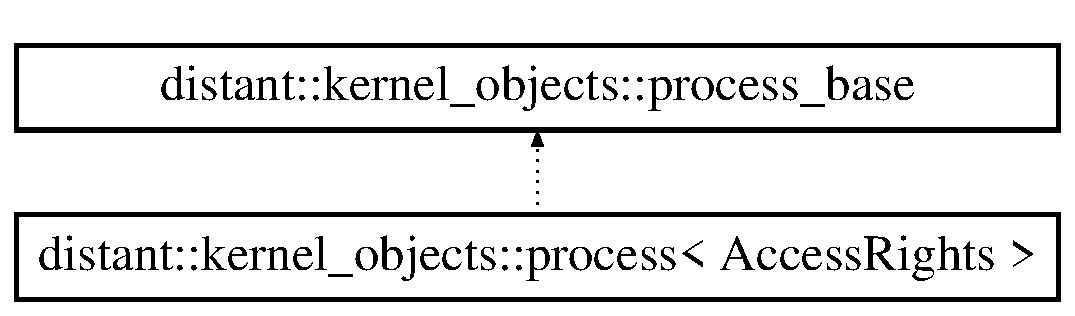
\includegraphics[height=2.000000cm]{classdistant_1_1kernel__objects_1_1process}
\end{center}
\end{figure}
\subsection*{Public Member Functions}
\begin{DoxyCompactItemize}
\item 
{\footnotesize template$<$typename Return  = void$>$ }\\auto \mbox{\hyperlink{classdistant_1_1kernel__objects_1_1process_a5740aade7f116777a17c84375b8643d2}{kill}} () -\/$>$ require\+\_\+permission$<$ process\+\_\+rights\+::terminate, Return $>$
\begin{DoxyCompactList}\small\item\em Terminate the process. \end{DoxyCompactList}\item 
{\footnotesize template$<$typename Return  = std\+::size\+\_\+t$>$ }\\auto \mbox{\hyperlink{classdistant_1_1kernel__objects_1_1process_a4db8ac7a1b08736c7b862862b02106c3}{handle\+\_\+count}} () const -\/$>$ require\+\_\+permission$<$ process\+\_\+rights\+::query\+\_\+limited\+\_\+information, Return $>$
\begin{DoxyCompactList}\small\item\em Get number of handles opened in the process. \end{DoxyCompactList}\item 
{\footnotesize template$<$typename Return  = bool$>$ }\\auto \mbox{\hyperlink{classdistant_1_1kernel__objects_1_1process_a40cfceaaded5c5f2a4c0ddc9cde8107e}{is\+\_\+active}} () const -\/$>$ require\+\_\+permission$<$ process\+\_\+rights\+::synchronize, Return $>$
\begin{DoxyCompactList}\small\item\em Query the process handle to see if it is still active. \end{DoxyCompactList}\item 
{\footnotesize template$<$typename Return  = bool$>$ }\\auto \mbox{\hyperlink{classdistant_1_1kernel__objects_1_1process_ae78ed9e64b111eee962f2fdaf59630ed}{is\+\_\+32bit}} () const -\/$>$ require\+\_\+permission$<$ process\+\_\+rights\+::query\+\_\+information$\vert$process\+\_\+rights\+::query\+\_\+limited\+\_\+information, Return $>$
\begin{DoxyCompactList}\small\item\em Test if the process is running under the W\+O\+W64 emulator. ~\newline
 If the process has been compiled to run on 32-\/bit system and is being run on a 64-\/bit system, it will be emulated. \end{DoxyCompactList}\item 
{\footnotesize template$<$typename Return  = bool$>$ }\\auto \mbox{\hyperlink{classdistant_1_1kernel__objects_1_1process_a9fc52566aa890d371eaedf82ad7a4868}{is\+\_\+64bit}} () const -\/$>$ require\+\_\+permission$<$ process\+\_\+rights\+::query\+\_\+information$\vert$process\+\_\+rights\+::query\+\_\+limited\+\_\+information, Return $>$
\begin{DoxyCompactList}\small\item\em Test if the process is being run in 64bit. \end{DoxyCompactList}\item 
{\footnotesize template$<$typename Return  = std\+::wstring$>$ }\\auto \mbox{\hyperlink{classdistant_1_1kernel__objects_1_1process_a380d7b1f70e856105848af6a9ae60d88}{name}} () const -\/$>$ require\+\_\+permission$<$ process\+\_\+rights\+::query\+\_\+information$\vert$process\+\_\+rights\+::query\+\_\+limited\+\_\+information, Return $>$
\begin{DoxyCompactList}\small\item\em Get the executable name of the process. \end{DoxyCompactList}\item 
{\footnotesize template$<$typename Return  = filesystem\+::path$>$ }\\auto \mbox{\hyperlink{classdistant_1_1kernel__objects_1_1process_abf8afdafb3ff75722ea2660aac7a7b22}{file\+\_\+path}} () const -\/$>$ require\+\_\+permission$<$ process\+\_\+rights\+::query\+\_\+information$\vert$process\+\_\+rights\+::query\+\_\+limited\+\_\+information, Return $>$
\begin{DoxyCompactList}\small\item\em Get the file path (in W\+I\+N32 format) of the process. \end{DoxyCompactList}\item 
\mbox{\Hypertarget{classdistant_1_1kernel__objects_1_1process_a2f6fbe7adb69ff892c305909545e15ab}\label{classdistant_1_1kernel__objects_1_1process_a2f6fbe7adb69ff892c305909545e15ab}} 
{\footnotesize template$<$process\+\_\+rights Other\+Access$>$ }\\\mbox{\hyperlink{classdistant_1_1kernel__objects_1_1process_a2f6fbe7adb69ff892c305909545e15ab}{operator process$<$ Other\+Access $>$ \&}} () noexcept
\begin{DoxyCompactList}\small\item\em Allows implicit conversion to a process with a lower level of access. \end{DoxyCompactList}\item 
\mbox{\Hypertarget{classdistant_1_1kernel__objects_1_1process_a7afdbe9eefdb12fe7c8cc5462b29ddcf}\label{classdistant_1_1kernel__objects_1_1process_a7afdbe9eefdb12fe7c8cc5462b29ddcf}} 
{\footnotesize template$<$process\+\_\+rights Other\+Access$>$ }\\\mbox{\hyperlink{classdistant_1_1kernel__objects_1_1process_a7afdbe9eefdb12fe7c8cc5462b29ddcf}{operator const process$<$ Other\+Access $>$ \&}} () const noexcept
\begin{DoxyCompactList}\small\item\em Allows implicit conversion to a process with a lower level of access. \end{DoxyCompactList}\item 
\mbox{\Hypertarget{classdistant_1_1kernel__objects_1_1process_a4df811c0599821d9c6940abb44162790}\label{classdistant_1_1kernel__objects_1_1process_a4df811c0599821d9c6940abb44162790}} 
constexpr \mbox{\hyperlink{classdistant_1_1kernel__objects_1_1process_a4df811c0599821d9c6940abb44162790}{process}} () noexcept
\begin{DoxyCompactList}\small\item\em Default process constructor. \end{DoxyCompactList}\item 
\mbox{\Hypertarget{classdistant_1_1kernel__objects_1_1process_a3006196cbaf28858afb6f6185f05b6f0}\label{classdistant_1_1kernel__objects_1_1process_a3006196cbaf28858afb6f6185f05b6f0}} 
\mbox{\hyperlink{classdistant_1_1kernel__objects_1_1process_a3006196cbaf28858afb6f6185f05b6f0}{process}} (std\+::size\+\_\+t \mbox{\hyperlink{classdistant_1_1kernel__objects_1_1process__base_a553b90767de864164d807075f67c1402}{id}}) noexcept
\begin{DoxyCompactList}\small\item\em Open process by id. \end{DoxyCompactList}\item 
\mbox{\Hypertarget{classdistant_1_1kernel__objects_1_1process_a7366312910893bf4ad49d947bc0fb172}\label{classdistant_1_1kernel__objects_1_1process_a7366312910893bf4ad49d947bc0fb172}} 
\mbox{\hyperlink{classdistant_1_1kernel__objects_1_1process_a7366312910893bf4ad49d947bc0fb172}{process}} (\mbox{\hyperlink{classdistant_1_1kernel__objects_1_1process}{process}} \&\&other) noexcept
\begin{DoxyCompactList}\small\item\em Move constructible. \end{DoxyCompactList}\item 
\mbox{\Hypertarget{classdistant_1_1kernel__objects_1_1process_aacea90575aaa7e9c84e2f80fa93fe62f}\label{classdistant_1_1kernel__objects_1_1process_aacea90575aaa7e9c84e2f80fa93fe62f}} 
\mbox{\hyperlink{classdistant_1_1kernel__objects_1_1process}{process}} \& \mbox{\hyperlink{classdistant_1_1kernel__objects_1_1process_aacea90575aaa7e9c84e2f80fa93fe62f}{operator=}} (\mbox{\hyperlink{classdistant_1_1kernel__objects_1_1process}{process}} \&\&other) noexcept
\begin{DoxyCompactList}\small\item\em Move assignable. \end{DoxyCompactList}\item 
\mbox{\Hypertarget{classdistant_1_1kernel__objects_1_1process_a83240e5580484794f24fcd57851e8c6f}\label{classdistant_1_1kernel__objects_1_1process_a83240e5580484794f24fcd57851e8c6f}} 
{\bfseries process} (\mbox{\hyperlink{classdistant_1_1handle}{distant\+::handle}}$<$ \mbox{\hyperlink{classdistant_1_1kernel__objects_1_1process}{process}} $>$ \&\&\mbox{\hyperlink{classdistant_1_1handle}{handle}}) noexcept
\item 
\mbox{\Hypertarget{classdistant_1_1kernel__objects_1_1process_a02b13d92ae5626f6816b3b17cb930cc3}\label{classdistant_1_1kernel__objects_1_1process_a02b13d92ae5626f6816b3b17cb930cc3}} 
{\footnotesize template$<$process\+\_\+rights Other\+Access, typename $>$ }\\{\bfseries operator process$<$ Other\+Access $>$ \&} () noexcept
\item 
\mbox{\Hypertarget{classdistant_1_1kernel__objects_1_1process_aed99eb2084963e9fe73278f845f2da39}\label{classdistant_1_1kernel__objects_1_1process_aed99eb2084963e9fe73278f845f2da39}} 
{\footnotesize template$<$process\+\_\+rights Other\+Access, typename $>$ }\\{\bfseries operator const process$<$ Other\+Access $>$ \&} () const noexcept
\item 
bool \mbox{\hyperlink{classdistant_1_1kernel__objects_1_1process_a9acb308895639407b1925ad238f05344}{is\+\_\+being\+\_\+debugged}} () const
\begin{DoxyCompactList}\small\item\em Test if the process is being debugged by another process. \end{DoxyCompactList}\item 
flag\+\_\+type \mbox{\hyperlink{classdistant_1_1kernel__objects_1_1process_a28b2a7b7297714d4c7c4d320a0c4fbbc}{access\+\_\+rights}} () const noexcept
\begin{DoxyCompactList}\small\item\em Get the access rights that were used to open the current process. \end{DoxyCompactList}\item 
\mbox{\Hypertarget{classdistant_1_1kernel__objects_1_1process_a3476af5b30ce778a41eed891fdd93ece}\label{classdistant_1_1kernel__objects_1_1process_a3476af5b30ce778a41eed891fdd93ece}} 
const \mbox{\hyperlink{classdistant_1_1handle}{distant\+::handle}}$<$ \mbox{\hyperlink{classdistant_1_1kernel__objects_1_1process__base}{process\+\_\+base}} $>$ \& {\bfseries handle} () const noexcept
\item 
bool \mbox{\hyperlink{classdistant_1_1kernel__objects_1_1process_ab023cd4a4d27ccef7879d1a3c513148b}{is\+\_\+zombie}} () const
\begin{DoxyCompactList}\small\item\em Test if the process is a \char`\"{}zombie\char`\"{} process. A zombie process in this case is one that is not listed upon process list enumeration, but still has an active handle in the operating system. \end{DoxyCompactList}\item 
bool \mbox{\hyperlink{classdistant_1_1kernel__objects_1_1process_a6299b49ad8fb1c22e54dc9aa6c3a09b2}{valid}} () const noexcept
\begin{DoxyCompactList}\small\item\em Test if the process \mbox{\hyperlink{classdistant_1_1kernel__objects_1_1kernel__object}{kernel\+\_\+object}} is valid. \end{DoxyCompactList}\item 
std\+::size\+\_\+t \mbox{\hyperlink{classdistant_1_1kernel__objects_1_1process_a553b90767de864164d807075f67c1402}{id}} () const noexcept
\begin{DoxyCompactList}\small\item\em Retrieve the process id. \end{DoxyCompactList}\end{DoxyCompactItemize}
\subsection*{Friends}
\begin{DoxyCompactItemize}
\item 
\mbox{\Hypertarget{classdistant_1_1kernel__objects_1_1process_adaff6948d20e49253266449bb112a8e8}\label{classdistant_1_1kernel__objects_1_1process_adaff6948d20e49253266449bb112a8e8}} 
class {\bfseries memory\+\_\+status}
\end{DoxyCompactItemize}


\subsection{Detailed Description}
\subsubsection*{template$<$process\+\_\+rights Access\+Rights = process\+\_\+rights\+::all\+\_\+access$>$\newline
class distant\+::kernel\+\_\+objects\+::process$<$ Access\+Rights $>$}

distant\+::process represents a process, and has static type checking on the process access rights. 


\begin{DoxyTemplParams}{Template Parameters}
{\em Access\+Rights} & the desired permissions to open the process with. \\
\hline
\end{DoxyTemplParams}
\begin{DoxySeeAlso}{See also}
process\+\_\+rights 
\end{DoxySeeAlso}


\subsection{Member Function Documentation}
\mbox{\Hypertarget{classdistant_1_1kernel__objects_1_1process_a28b2a7b7297714d4c7c4d320a0c4fbbc}\label{classdistant_1_1kernel__objects_1_1process_a28b2a7b7297714d4c7c4d320a0c4fbbc}} 
\index{distant\+::kernel\+\_\+objects\+::process@{distant\+::kernel\+\_\+objects\+::process}!access\+\_\+rights@{access\+\_\+rights}}
\index{access\+\_\+rights@{access\+\_\+rights}!distant\+::kernel\+\_\+objects\+::process@{distant\+::kernel\+\_\+objects\+::process}}
\subsubsection{\texorpdfstring{access\+\_\+rights()}{access\_rights()}}
{\footnotesize\ttfamily template$<$process\+\_\+rights Access\+Rights = process\+\_\+rights\+::all\+\_\+access$>$ \\
flag\+\_\+type distant\+::kernel\+\_\+objects\+::process\+\_\+base\+::access\+\_\+rights\hspace{0.3cm}{\ttfamily [inline]}, {\ttfamily [noexcept]}}



Get the access rights that were used to open the current process. 

\begin{DoxyReturn}{Returns}
process \mbox{\hyperlink{structdistant_1_1access__rights}{access\+\_\+rights}} indicating the level of access we have to the process. 
\end{DoxyReturn}
\mbox{\Hypertarget{classdistant_1_1kernel__objects_1_1process_abf8afdafb3ff75722ea2660aac7a7b22}\label{classdistant_1_1kernel__objects_1_1process_abf8afdafb3ff75722ea2660aac7a7b22}} 
\index{distant\+::kernel\+\_\+objects\+::process@{distant\+::kernel\+\_\+objects\+::process}!file\+\_\+path@{file\+\_\+path}}
\index{file\+\_\+path@{file\+\_\+path}!distant\+::kernel\+\_\+objects\+::process@{distant\+::kernel\+\_\+objects\+::process}}
\subsubsection{\texorpdfstring{file\+\_\+path()}{file\_path()}}
{\footnotesize\ttfamily template$<$access\+\_\+rights\+::process T$>$ \\
template$<$typename Return $>$ \\
auto \mbox{\hyperlink{classdistant_1_1kernel__objects_1_1process}{distant\+::kernel\+\_\+objects\+::process}}$<$ T $>$\+::file\+\_\+path (\begin{DoxyParamCaption}{ }\end{DoxyParamCaption}) const -\/$>$ require\+\_\+permission$<$process\+\_\+rights\+::query\+\_\+information $\vert$ process\+\_\+rights\+::query\+\_\+limited\+\_\+information, Return$>$}



Get the file path (in W\+I\+N32 format) of the process. 

\begin{DoxySeeAlso}{See also}
process\+\_\+rights 
\end{DoxySeeAlso}
\begin{DoxyReturn}{Returns}
filesystem\+::path\+: the absolute path to the executable image for the given process. 
\end{DoxyReturn}
\begin{DoxyRemark}{Remarks}
Requires {\itshape Access\+Rights} $>$= {\itshape query\+\_\+limited\+\_\+information} or {\itshape Access\+Rights} $>$= {\itshape query\+\_\+information}. 
\end{DoxyRemark}
\mbox{\Hypertarget{classdistant_1_1kernel__objects_1_1process_a4db8ac7a1b08736c7b862862b02106c3}\label{classdistant_1_1kernel__objects_1_1process_a4db8ac7a1b08736c7b862862b02106c3}} 
\index{distant\+::kernel\+\_\+objects\+::process@{distant\+::kernel\+\_\+objects\+::process}!handle\+\_\+count@{handle\+\_\+count}}
\index{handle\+\_\+count@{handle\+\_\+count}!distant\+::kernel\+\_\+objects\+::process@{distant\+::kernel\+\_\+objects\+::process}}
\subsubsection{\texorpdfstring{handle\+\_\+count()}{handle\_count()}}
{\footnotesize\ttfamily template$<$access\+\_\+rights\+::process T$>$ \\
template$<$typename Return $>$ \\
auto \mbox{\hyperlink{classdistant_1_1kernel__objects_1_1process}{distant\+::kernel\+\_\+objects\+::process}}$<$ T $>$\+::handle\+\_\+count (\begin{DoxyParamCaption}{ }\end{DoxyParamCaption}) const -\/$>$ require\+\_\+permission$<$process\+\_\+rights\+::query\+\_\+limited\+\_\+information, Return$>$}



Get number of handles opened in the process. 

\begin{DoxySeeAlso}{See also}
process\+\_\+rights 
\end{DoxySeeAlso}
\begin{DoxyReturn}{Returns}
unsigned int\+: the number of handles 
\end{DoxyReturn}
\begin{DoxyRemark}{Remarks}
Requires {\itshape Access\+Rights} $>$= {\itshape query\+\_\+limited\+\_\+information}. 
\end{DoxyRemark}
\mbox{\Hypertarget{classdistant_1_1kernel__objects_1_1process_a553b90767de864164d807075f67c1402}\label{classdistant_1_1kernel__objects_1_1process_a553b90767de864164d807075f67c1402}} 
\index{distant\+::kernel\+\_\+objects\+::process@{distant\+::kernel\+\_\+objects\+::process}!id@{id}}
\index{id@{id}!distant\+::kernel\+\_\+objects\+::process@{distant\+::kernel\+\_\+objects\+::process}}
\subsubsection{\texorpdfstring{id()}{id()}}
{\footnotesize\ttfamily template$<$process\+\_\+rights Access\+Rights = process\+\_\+rights\+::all\+\_\+access$>$ \\
std\+::size\+\_\+t distant\+::kernel\+\_\+objects\+::process\+\_\+base\+::id\hspace{0.3cm}{\ttfamily [inline]}, {\ttfamily [noexcept]}}



Retrieve the process id. 

\begin{DoxyReturn}{Returns}
the process id. 
\end{DoxyReturn}
\mbox{\Hypertarget{classdistant_1_1kernel__objects_1_1process_ae78ed9e64b111eee962f2fdaf59630ed}\label{classdistant_1_1kernel__objects_1_1process_ae78ed9e64b111eee962f2fdaf59630ed}} 
\index{distant\+::kernel\+\_\+objects\+::process@{distant\+::kernel\+\_\+objects\+::process}!is\+\_\+32bit@{is\+\_\+32bit}}
\index{is\+\_\+32bit@{is\+\_\+32bit}!distant\+::kernel\+\_\+objects\+::process@{distant\+::kernel\+\_\+objects\+::process}}
\subsubsection{\texorpdfstring{is\+\_\+32bit()}{is\_32bit()}}
{\footnotesize\ttfamily template$<$access\+\_\+rights\+::process T$>$ \\
template$<$typename Return $>$ \\
auto \mbox{\hyperlink{classdistant_1_1kernel__objects_1_1process}{distant\+::kernel\+\_\+objects\+::process}}$<$ T $>$\+::is\+\_\+32bit (\begin{DoxyParamCaption}{ }\end{DoxyParamCaption}) const -\/$>$ require\+\_\+permission$<$process\+\_\+rights\+::query\+\_\+information $\vert$ process\+\_\+rights\+::query\+\_\+limited\+\_\+information, Return$>$}



Test if the process is running under the W\+O\+W64 emulator. ~\newline
 If the process has been compiled to run on 32-\/bit system and is being run on a 64-\/bit system, it will be emulated. 

\begin{DoxySeeAlso}{See also}
process\+\_\+rights 
\end{DoxySeeAlso}
\begin{DoxyReturn}{Returns}
bool\+: {\itshape true} if the process is being emulated, and {\itshape false} otherwise. 
\end{DoxyReturn}
\begin{DoxyRemark}{Remarks}
Requires {\itshape Access\+Rights} $>$= {\itshape query\+\_\+limited\+\_\+information} or {\itshape Access\+Rights} $>$= {\itshape query\+\_\+information}. 
\end{DoxyRemark}
\mbox{\Hypertarget{classdistant_1_1kernel__objects_1_1process_a9fc52566aa890d371eaedf82ad7a4868}\label{classdistant_1_1kernel__objects_1_1process_a9fc52566aa890d371eaedf82ad7a4868}} 
\index{distant\+::kernel\+\_\+objects\+::process@{distant\+::kernel\+\_\+objects\+::process}!is\+\_\+64bit@{is\+\_\+64bit}}
\index{is\+\_\+64bit@{is\+\_\+64bit}!distant\+::kernel\+\_\+objects\+::process@{distant\+::kernel\+\_\+objects\+::process}}
\subsubsection{\texorpdfstring{is\+\_\+64bit()}{is\_64bit()}}
{\footnotesize\ttfamily template$<$access\+\_\+rights\+::process T$>$ \\
template$<$typename Return $>$ \\
auto \mbox{\hyperlink{classdistant_1_1kernel__objects_1_1process}{distant\+::kernel\+\_\+objects\+::process}}$<$ T $>$\+::is\+\_\+64bit (\begin{DoxyParamCaption}{ }\end{DoxyParamCaption}) const -\/$>$ require\+\_\+permission$<$process\+\_\+rights\+::query\+\_\+information $\vert$ process\+\_\+rights\+::query\+\_\+limited\+\_\+information, Return$>$}



Test if the process is being run in 64bit. 

\begin{DoxySeeAlso}{See also}
process\+\_\+rights 
\end{DoxySeeAlso}
\begin{DoxyReturn}{Returns}
bool\+: {\itshape true} if the process is being run in 64bit mode, and {\itshape false} otherwise. 
\end{DoxyReturn}
\begin{DoxyRemark}{Remarks}
Requires {\itshape Access\+Rights} $>$= {\itshape query\+\_\+limited\+\_\+information} or {\itshape Access\+Rights} $>$= {\itshape query\+\_\+information}. 
\end{DoxyRemark}
\mbox{\Hypertarget{classdistant_1_1kernel__objects_1_1process_a40cfceaaded5c5f2a4c0ddc9cde8107e}\label{classdistant_1_1kernel__objects_1_1process_a40cfceaaded5c5f2a4c0ddc9cde8107e}} 
\index{distant\+::kernel\+\_\+objects\+::process@{distant\+::kernel\+\_\+objects\+::process}!is\+\_\+active@{is\+\_\+active}}
\index{is\+\_\+active@{is\+\_\+active}!distant\+::kernel\+\_\+objects\+::process@{distant\+::kernel\+\_\+objects\+::process}}
\subsubsection{\texorpdfstring{is\+\_\+active()}{is\_active()}}
{\footnotesize\ttfamily template$<$access\+\_\+rights\+::process T$>$ \\
template$<$typename Return $>$ \\
auto \mbox{\hyperlink{classdistant_1_1kernel__objects_1_1process}{distant\+::kernel\+\_\+objects\+::process}}$<$ T $>$\+::is\+\_\+active (\begin{DoxyParamCaption}{ }\end{DoxyParamCaption}) const -\/$>$ require\+\_\+permission$<$process\+\_\+rights\+::synchronize, Return$>$}



Query the process handle to see if it is still active. 

\begin{DoxySeeAlso}{See also}
process\+\_\+rights 
\end{DoxySeeAlso}
\begin{DoxyReturn}{Returns}
bool\+: {\itshape true} if the process is active, and {\itshape false} otherwise 
\end{DoxyReturn}
\begin{DoxyRemark}{Remarks}
Requires {\itshape Access\+Rights} $>$= {\itshape synchronize}. 
\end{DoxyRemark}
\mbox{\Hypertarget{classdistant_1_1kernel__objects_1_1process_a9acb308895639407b1925ad238f05344}\label{classdistant_1_1kernel__objects_1_1process_a9acb308895639407b1925ad238f05344}} 
\index{distant\+::kernel\+\_\+objects\+::process@{distant\+::kernel\+\_\+objects\+::process}!is\+\_\+being\+\_\+debugged@{is\+\_\+being\+\_\+debugged}}
\index{is\+\_\+being\+\_\+debugged@{is\+\_\+being\+\_\+debugged}!distant\+::kernel\+\_\+objects\+::process@{distant\+::kernel\+\_\+objects\+::process}}
\subsubsection{\texorpdfstring{is\+\_\+being\+\_\+debugged()}{is\_being\_debugged()}}
{\footnotesize\ttfamily template$<$process\+\_\+rights Access\+Rights = process\+\_\+rights\+::all\+\_\+access$>$ \\
bool distant\+::kernel\+\_\+objects\+::process\+\_\+base\+::is\+\_\+being\+\_\+debugged\hspace{0.3cm}{\ttfamily [inline]}}



Test if the process is being debugged by another process. 

\begin{DoxyReturn}{Returns}
true if the process is being debugged, and false if it is not. 
\end{DoxyReturn}
\mbox{\Hypertarget{classdistant_1_1kernel__objects_1_1process_ab023cd4a4d27ccef7879d1a3c513148b}\label{classdistant_1_1kernel__objects_1_1process_ab023cd4a4d27ccef7879d1a3c513148b}} 
\index{distant\+::kernel\+\_\+objects\+::process@{distant\+::kernel\+\_\+objects\+::process}!is\+\_\+zombie@{is\+\_\+zombie}}
\index{is\+\_\+zombie@{is\+\_\+zombie}!distant\+::kernel\+\_\+objects\+::process@{distant\+::kernel\+\_\+objects\+::process}}
\subsubsection{\texorpdfstring{is\+\_\+zombie()}{is\_zombie()}}
{\footnotesize\ttfamily template$<$process\+\_\+rights Access\+Rights = process\+\_\+rights\+::all\+\_\+access$>$ \\
bool distant\+::kernel\+\_\+objects\+::process\+\_\+base\+::is\+\_\+zombie\hspace{0.3cm}{\ttfamily [inline]}}



Test if the process is a \char`\"{}zombie\char`\"{} process. A zombie process in this case is one that is not listed upon process list enumeration, but still has an active handle in the operating system. 

\begin{DoxyReturn}{Returns}
true if the process is a zombie. 
\end{DoxyReturn}
\mbox{\Hypertarget{classdistant_1_1kernel__objects_1_1process_a5740aade7f116777a17c84375b8643d2}\label{classdistant_1_1kernel__objects_1_1process_a5740aade7f116777a17c84375b8643d2}} 
\index{distant\+::kernel\+\_\+objects\+::process@{distant\+::kernel\+\_\+objects\+::process}!kill@{kill}}
\index{kill@{kill}!distant\+::kernel\+\_\+objects\+::process@{distant\+::kernel\+\_\+objects\+::process}}
\subsubsection{\texorpdfstring{kill()}{kill()}}
{\footnotesize\ttfamily template$<$access\+\_\+rights\+::process T$>$ \\
template$<$typename Return $>$ \\
auto \mbox{\hyperlink{classdistant_1_1kernel__objects_1_1process}{distant\+::kernel\+\_\+objects\+::process}}$<$ T $>$\+::kill (\begin{DoxyParamCaption}{ }\end{DoxyParamCaption}) -\/$>$ require\+\_\+permission$<$process\+\_\+rights\+::terminate, Return$>$}



Terminate the process. 

\begin{DoxySeeAlso}{See also}
process\+\_\+rights 
\end{DoxySeeAlso}
\begin{DoxyRemark}{Remarks}
Requires {\itshape Access\+Rights} $>$= {\itshape terminate}. 
\end{DoxyRemark}
\mbox{\Hypertarget{classdistant_1_1kernel__objects_1_1process_a380d7b1f70e856105848af6a9ae60d88}\label{classdistant_1_1kernel__objects_1_1process_a380d7b1f70e856105848af6a9ae60d88}} 
\index{distant\+::kernel\+\_\+objects\+::process@{distant\+::kernel\+\_\+objects\+::process}!name@{name}}
\index{name@{name}!distant\+::kernel\+\_\+objects\+::process@{distant\+::kernel\+\_\+objects\+::process}}
\subsubsection{\texorpdfstring{name()}{name()}}
{\footnotesize\ttfamily template$<$access\+\_\+rights\+::process T$>$ \\
template$<$typename Return $>$ \\
auto \mbox{\hyperlink{classdistant_1_1kernel__objects_1_1process}{distant\+::kernel\+\_\+objects\+::process}}$<$ T $>$\+::name (\begin{DoxyParamCaption}{ }\end{DoxyParamCaption}) const -\/$>$ require\+\_\+permission$<$process\+\_\+rights\+::query\+\_\+information $\vert$ process\+\_\+rights\+::query\+\_\+limited\+\_\+information, Return$>$}



Get the executable name of the process. 

\begin{DoxySeeAlso}{See also}
process\+\_\+rights 
\end{DoxySeeAlso}
\begin{DoxyReturn}{Returns}
std\+::wstring\+: the executable image name for the given process. 
\end{DoxyReturn}
\begin{DoxyRemark}{Remarks}
Requires {\itshape Access\+Rights} $>$= {\itshape query\+\_\+limited\+\_\+information} or {\itshape Access\+Rights} $>$= {\itshape query\+\_\+information}. 
\end{DoxyRemark}
\mbox{\Hypertarget{classdistant_1_1kernel__objects_1_1process_a6299b49ad8fb1c22e54dc9aa6c3a09b2}\label{classdistant_1_1kernel__objects_1_1process_a6299b49ad8fb1c22e54dc9aa6c3a09b2}} 
\index{distant\+::kernel\+\_\+objects\+::process@{distant\+::kernel\+\_\+objects\+::process}!valid@{valid}}
\index{valid@{valid}!distant\+::kernel\+\_\+objects\+::process@{distant\+::kernel\+\_\+objects\+::process}}
\subsubsection{\texorpdfstring{valid()}{valid()}}
{\footnotesize\ttfamily template$<$process\+\_\+rights Access\+Rights = process\+\_\+rights\+::all\+\_\+access$>$ \\
bool distant\+::kernel\+\_\+objects\+::process\+\_\+base\+::valid\hspace{0.3cm}{\ttfamily [inline]}, {\ttfamily [noexcept]}}



Test if the process \mbox{\hyperlink{classdistant_1_1kernel__objects_1_1kernel__object}{kernel\+\_\+object}} is valid. 

\begin{DoxyReturn}{Returns}
true if the process is valid, false otherwise. 
\end{DoxyReturn}


The documentation for this class was generated from the following files\+:\begin{DoxyCompactItemize}
\item 
C\+:/\+Users/dinne/source/repos/distant dev/distant dev/include/distant/kernel\+\_\+objects/fwd.\+hpp\item 
C\+:/\+Users/dinne/source/repos/distant dev/distant dev/include/distant/kernel\+\_\+objects/process.\+hpp\item 
C\+:/\+Users/dinne/source/repos/distant dev/distant dev/include/distant/kernel\+\_\+objects/impl/process.\+hxx\end{DoxyCompactItemize}

\hypertarget{classdistant_1_1kernel__objects_1_1process__base}{}\section{distant\+:\+:kernel\+\_\+objects\+:\+:process\+\_\+base Class Reference}
\label{classdistant_1_1kernel__objects_1_1process__base}\index{distant\+::kernel\+\_\+objects\+::process\+\_\+base@{distant\+::kernel\+\_\+objects\+::process\+\_\+base}}


Base type of distant\+::process This version does not have static \mbox{\hyperlink{structdistant_1_1access__rights}{access\+\_\+rights}} checking.  




{\ttfamily \#include $<$process\+\_\+base.\+hpp$>$}

Inheritance diagram for distant\+:\+:kernel\+\_\+objects\+:\+:process\+\_\+base\+:\begin{figure}[H]
\begin{center}
\leavevmode
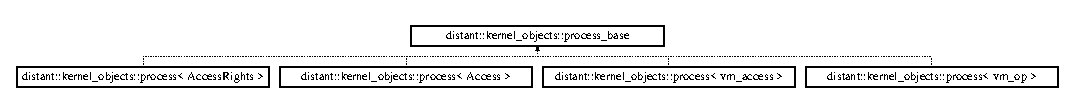
\includegraphics[height=0.949153cm]{classdistant_1_1kernel__objects_1_1process__base}
\end{center}
\end{figure}
\subsection*{Public Types}
\begin{DoxyCompactItemize}
\item 
\mbox{\Hypertarget{classdistant_1_1kernel__objects_1_1process__base_a2bbdf1b2c69e2f076aba267294dac8a5}\label{classdistant_1_1kernel__objects_1_1process__base_a2bbdf1b2c69e2f076aba267294dac8a5}} 
using {\bfseries base\+\_\+type} = \mbox{\hyperlink{classdistant_1_1kernel__objects_1_1kernel__object}{kernel\+\_\+object}}
\item 
\mbox{\Hypertarget{classdistant_1_1kernel__objects_1_1process__base_af6e123be2cae7818d2695fd98a904f1e}\label{classdistant_1_1kernel__objects_1_1process__base_af6e123be2cae7818d2695fd98a904f1e}} 
using {\bfseries error\+\_\+type} = \mbox{\hyperlink{structdistant_1_1kernel__object__traits}{kernel\+\_\+object\+\_\+traits}}$<$ \mbox{\hyperlink{classdistant_1_1kernel__objects_1_1process__base}{process\+\_\+base}} $>$\+::\mbox{\hyperlink{classdistant_1_1error_1_1windows__error__code}{error\+\_\+type}}
\item 
\mbox{\Hypertarget{classdistant_1_1kernel__objects_1_1process__base_a8dc331497fcc1d116c595bf412b0b6c8}\label{classdistant_1_1kernel__objects_1_1process__base_a8dc331497fcc1d116c595bf412b0b6c8}} 
using {\bfseries handle\+\_\+type} = \mbox{\hyperlink{structdistant_1_1kernel__object__traits}{kernel\+\_\+object\+\_\+traits}}$<$ \mbox{\hyperlink{classdistant_1_1kernel__objects_1_1process__base}{process\+\_\+base}} $>$\+::\mbox{\hyperlink{classdistant_1_1handle}{handle\+\_\+type}}
\item 
\mbox{\Hypertarget{classdistant_1_1kernel__objects_1_1process__base_a167dca0d4baabe8ca206b2e6e1b03282}\label{classdistant_1_1kernel__objects_1_1process__base_a167dca0d4baabe8ca206b2e6e1b03282}} 
using {\bfseries native\+\_\+handle\+\_\+type} = \mbox{\hyperlink{structdistant_1_1kernel__object__traits}{kernel\+\_\+object\+\_\+traits}}$<$ \mbox{\hyperlink{classdistant_1_1kernel__objects_1_1process__base}{process\+\_\+base}} $>$\+::native\+\_\+handle\+\_\+type
\item 
\mbox{\Hypertarget{classdistant_1_1kernel__objects_1_1process__base_a551a3e72af7a0c58c6b4eb4f6c4f7d0e}\label{classdistant_1_1kernel__objects_1_1process__base_a551a3e72af7a0c58c6b4eb4f6c4f7d0e}} 
using {\bfseries access\+\_\+rights\+\_\+t} = process\+\_\+rights
\item 
\mbox{\Hypertarget{classdistant_1_1kernel__objects_1_1process__base_a66d761572fa3db89575a79d396277667}\label{classdistant_1_1kernel__objects_1_1process__base_a66d761572fa3db89575a79d396277667}} 
using {\bfseries flag\+\_\+type} = access\+\_\+rights\+\_\+t
\end{DoxyCompactItemize}
\subsection*{Public Member Functions}
\begin{DoxyCompactItemize}
\item 
\mbox{\Hypertarget{classdistant_1_1kernel__objects_1_1process__base_a3f1bf976485f4c55ab5e12b972382836}\label{classdistant_1_1kernel__objects_1_1process__base_a3f1bf976485f4c55ab5e12b972382836}} 
void \mbox{\hyperlink{classdistant_1_1kernel__objects_1_1process__base_a3f1bf976485f4c55ab5e12b972382836}{kill}} ()
\begin{DoxyCompactList}\small\item\em Terminate the process. \end{DoxyCompactList}\item 
bool \mbox{\hyperlink{classdistant_1_1kernel__objects_1_1process__base_ac3d56fd3e4c92b1e1dbbf2f5f9242fbe}{is\+\_\+active}} () const
\begin{DoxyCompactList}\small\item\em Query the process handle to see if it is still active. \end{DoxyCompactList}\item 
bool \mbox{\hyperlink{classdistant_1_1kernel__objects_1_1process__base_a4c71065703937a737865428b03af8e99}{is\+\_\+32bit}} () const
\begin{DoxyCompactList}\small\item\em Test if the process is running under the W\+O\+W64 emulator. If the process has been compiled to run on 32-\/bit system and is being run on a 64-\/bit system, it will be emulated. \end{DoxyCompactList}\item 
bool \mbox{\hyperlink{classdistant_1_1kernel__objects_1_1process__base_a9ac787a611e73f5347cd25a850fa0122}{is\+\_\+64bit}} () const
\begin{DoxyCompactList}\small\item\em Test if the process is being run in 64bit. \end{DoxyCompactList}\item 
std\+::wstring \mbox{\hyperlink{classdistant_1_1kernel__objects_1_1process__base_a465314221bd0fbea3ce48ffcf7213578}{name}} () const
\begin{DoxyCompactList}\small\item\em Get the name of the process executable. \end{DoxyCompactList}\item 
filesystem\+::path \mbox{\hyperlink{classdistant_1_1kernel__objects_1_1process__base_a0c1640e125f4667c139bf9d44f7cd096}{file\+\_\+path}} () const
\begin{DoxyCompactList}\small\item\em Get the path to the process executable. \end{DoxyCompactList}\item 
bool \mbox{\hyperlink{classdistant_1_1kernel__objects_1_1process__base_a9acb308895639407b1925ad238f05344}{is\+\_\+being\+\_\+debugged}} () const
\begin{DoxyCompactList}\small\item\em Test if the process is being debugged by another process. \end{DoxyCompactList}\item 
bool \mbox{\hyperlink{classdistant_1_1kernel__objects_1_1process__base_ab023cd4a4d27ccef7879d1a3c513148b}{is\+\_\+zombie}} () const
\begin{DoxyCompactList}\small\item\em Test if the process is a \char`\"{}zombie\char`\"{} process. A zombie process in this case is one that is not listed upon process list enumeration, but still has an active handle in the operating system. \end{DoxyCompactList}\item 
std\+::size\+\_\+t \mbox{\hyperlink{classdistant_1_1kernel__objects_1_1process__base_a8c14c3aca084496eafa68f23b7535567}{handle\+\_\+count}} () const
\item 
std\+::size\+\_\+t \mbox{\hyperlink{classdistant_1_1kernel__objects_1_1process__base_a553b90767de864164d807075f67c1402}{id}} () const noexcept
\begin{DoxyCompactList}\small\item\em Retrieve the process id. \end{DoxyCompactList}\item 
\mbox{\Hypertarget{classdistant_1_1kernel__objects_1_1process__base_a3476af5b30ce778a41eed891fdd93ece}\label{classdistant_1_1kernel__objects_1_1process__base_a3476af5b30ce778a41eed891fdd93ece}} 
const \mbox{\hyperlink{classdistant_1_1handle}{distant\+::handle}}$<$ \mbox{\hyperlink{classdistant_1_1kernel__objects_1_1process__base}{process\+\_\+base}} $>$ \& {\bfseries handle} () const noexcept
\item 
flag\+\_\+type \mbox{\hyperlink{classdistant_1_1kernel__objects_1_1process__base_a28b2a7b7297714d4c7c4d320a0c4fbbc}{access\+\_\+rights}} () const noexcept
\begin{DoxyCompactList}\small\item\em Get the access rights that were used to open the current process. \end{DoxyCompactList}\item 
bool \mbox{\hyperlink{classdistant_1_1kernel__objects_1_1process__base_a6299b49ad8fb1c22e54dc9aa6c3a09b2}{valid}} () const noexcept
\begin{DoxyCompactList}\small\item\em Test if the process \mbox{\hyperlink{classdistant_1_1kernel__objects_1_1kernel__object}{kernel\+\_\+object}} is valid. \end{DoxyCompactList}\item 
\mbox{\hyperlink{classdistant_1_1kernel__objects_1_1process__base_a0d69c4e7d61551e7246eed5dcaabc6d9}{operator bool}} () const noexcept
\begin{DoxyCompactList}\small\item\em Test if the process \mbox{\hyperlink{classdistant_1_1kernel__objects_1_1kernel__object}{kernel\+\_\+object}} is valid. \end{DoxyCompactList}\item 
\mbox{\Hypertarget{classdistant_1_1kernel__objects_1_1process__base_ad5aa6b7591af9560bf164b5ae75a295c}\label{classdistant_1_1kernel__objects_1_1process__base_ad5aa6b7591af9560bf164b5ae75a295c}} 
\mbox{\hyperlink{classdistant_1_1kernel__objects_1_1process__base_ad5aa6b7591af9560bf164b5ae75a295c}{process\+\_\+base}} () noexcept
\begin{DoxyCompactList}\small\item\em Construct an empty process. \end{DoxyCompactList}\item 
\mbox{\hyperlink{classdistant_1_1kernel__objects_1_1process__base_a845358a2126f878a2777acf7d855b79b}{process\+\_\+base}} (std\+::size\+\_\+t \mbox{\hyperlink{classdistant_1_1kernel__objects_1_1process__base_a553b90767de864164d807075f67c1402}{id}}, access\+\_\+rights\+\_\+t access=access\+\_\+rights\+\_\+t\+::all\+\_\+access) noexcept
\begin{DoxyCompactList}\small\item\em Open process by id. \end{DoxyCompactList}\item 
\mbox{\Hypertarget{classdistant_1_1kernel__objects_1_1process__base_a77b9fe42db8ee2b364cf6e56f369867b}\label{classdistant_1_1kernel__objects_1_1process__base_a77b9fe42db8ee2b364cf6e56f369867b}} 
{\bfseries process\+\_\+base} (\mbox{\hyperlink{classdistant_1_1kernel__objects_1_1process__base}{process\+\_\+base}} \&\&other) noexcept
\item 
\mbox{\Hypertarget{classdistant_1_1kernel__objects_1_1process__base_a449fa10bee50a4091db59a6550479598}\label{classdistant_1_1kernel__objects_1_1process__base_a449fa10bee50a4091db59a6550479598}} 
\mbox{\hyperlink{classdistant_1_1kernel__objects_1_1process__base}{process\+\_\+base}} \& {\bfseries operator=} (\mbox{\hyperlink{classdistant_1_1kernel__objects_1_1process__base}{process\+\_\+base}} \&\&other) noexcept
\item 
\mbox{\Hypertarget{classdistant_1_1kernel__objects_1_1process__base_a80ae44cbed38950723309d0a567af7c1}\label{classdistant_1_1kernel__objects_1_1process__base_a80ae44cbed38950723309d0a567af7c1}} 
{\bfseries process\+\_\+base} (\mbox{\hyperlink{classdistant_1_1handle}{distant\+::handle}}$<$ \mbox{\hyperlink{classdistant_1_1kernel__objects_1_1process__base}{process\+\_\+base}} $>$ \&\&\mbox{\hyperlink{classdistant_1_1handle}{handle}}, access\+\_\+rights\+\_\+t) noexcept
\end{DoxyCompactItemize}
\subsection*{Static Protected Member Functions}
\begin{DoxyCompactItemize}
\item 
\mbox{\Hypertarget{classdistant_1_1kernel__objects_1_1process__base_a4bad2a3570c2e76ded4a8bd22f4928a9}\label{classdistant_1_1kernel__objects_1_1process__base_a4bad2a3570c2e76ded4a8bd22f4928a9}} 
static \mbox{\hyperlink{classdistant_1_1handle}{handle\+\_\+type}} {\bfseries open} (std\+::size\+\_\+t, access\+\_\+rights\+\_\+t) noexcept
\item 
\mbox{\Hypertarget{classdistant_1_1kernel__objects_1_1process__base_a7bec537ad007e7439f81fc95c965958d}\label{classdistant_1_1kernel__objects_1_1process__base_a7bec537ad007e7439f81fc95c965958d}} 
static std\+::size\+\_\+t {\bfseries get\+\_\+pid} (const \mbox{\hyperlink{classdistant_1_1handle}{handle\+\_\+type}} \&) noexcept
\end{DoxyCompactItemize}
\subsection*{Protected Attributes}
\begin{DoxyCompactItemize}
\item 
\mbox{\Hypertarget{classdistant_1_1kernel__objects_1_1process__base_aa2f7eeea4b9769e9ebda10d907fea830}\label{classdistant_1_1kernel__objects_1_1process__base_aa2f7eeea4b9769e9ebda10d907fea830}} 
\mbox{\hyperlink{classdistant_1_1handle}{distant\+::handle}}$<$ \mbox{\hyperlink{classdistant_1_1kernel__objects_1_1process__base}{process\+\_\+base}} $>$ {\bfseries handle\+\_\+}
\item 
\mbox{\Hypertarget{classdistant_1_1kernel__objects_1_1process__base_a7fb322f6d108727fb48a986ac88a3199}\label{classdistant_1_1kernel__objects_1_1process__base_a7fb322f6d108727fb48a986ac88a3199}} 
std\+::size\+\_\+t {\bfseries id\+\_\+}
\item 
\mbox{\Hypertarget{classdistant_1_1kernel__objects_1_1process__base_af4f78745cb41d78979cc313b6e91f3b3}\label{classdistant_1_1kernel__objects_1_1process__base_af4f78745cb41d78979cc313b6e91f3b3}} 
access\+\_\+rights\+\_\+t {\bfseries access\+\_\+rights\+\_\+}
\end{DoxyCompactItemize}
\subsection*{Friends}
\begin{DoxyCompactItemize}
\item 
\mbox{\Hypertarget{classdistant_1_1kernel__objects_1_1process__base_a023b8a425917f7dddc2144678a3d5bfb}\label{classdistant_1_1kernel__objects_1_1process__base_a023b8a425917f7dddc2144678a3d5bfb}} 
bool {\bfseries operator==} (const \mbox{\hyperlink{classdistant_1_1kernel__objects_1_1process__base}{process\+\_\+base}} \&, const \mbox{\hyperlink{classdistant_1_1kernel__objects_1_1process__base}{process\+\_\+base}} \&) noexcept
\item 
\mbox{\Hypertarget{classdistant_1_1kernel__objects_1_1process__base_a5fd7d7dcf5b09480ae8c4b742562db1a}\label{classdistant_1_1kernel__objects_1_1process__base_a5fd7d7dcf5b09480ae8c4b742562db1a}} 
bool {\bfseries operator!=} (const \mbox{\hyperlink{classdistant_1_1kernel__objects_1_1process__base}{process\+\_\+base}} \&, const \mbox{\hyperlink{classdistant_1_1kernel__objects_1_1process__base}{process\+\_\+base}} \&) noexcept
\end{DoxyCompactItemize}


\subsection{Detailed Description}
Base type of distant\+::process This version does not have static \mbox{\hyperlink{structdistant_1_1access__rights}{access\+\_\+rights}} checking. 

\subsection{Constructor \& Destructor Documentation}
\mbox{\Hypertarget{classdistant_1_1kernel__objects_1_1process__base_a845358a2126f878a2777acf7d855b79b}\label{classdistant_1_1kernel__objects_1_1process__base_a845358a2126f878a2777acf7d855b79b}} 
\index{distant\+::kernel\+\_\+objects\+::process\+\_\+base@{distant\+::kernel\+\_\+objects\+::process\+\_\+base}!process\+\_\+base@{process\+\_\+base}}
\index{process\+\_\+base@{process\+\_\+base}!distant\+::kernel\+\_\+objects\+::process\+\_\+base@{distant\+::kernel\+\_\+objects\+::process\+\_\+base}}
\subsubsection{\texorpdfstring{process\+\_\+base()}{process\_base()}}
{\footnotesize\ttfamily distant\+::kernel\+\_\+objects\+::process\+\_\+base\+::process\+\_\+base (\begin{DoxyParamCaption}\item[{std\+::size\+\_\+t}]{id,  }\item[{access\+\_\+rights\+\_\+t}]{access = {\ttfamily access\+\_\+rights\+\_\+t\+:\+:all\+\_\+access} }\end{DoxyParamCaption})\hspace{0.3cm}{\ttfamily [inline]}, {\ttfamily [explicit]}, {\ttfamily [noexcept]}}



Open process by id. 


\begin{DoxyParams}{Parameters}
{\em id} & the pid (process id) of the process to open. \\
\hline
{\em access} & the requested access rights to open the process with. \\
\hline
\end{DoxyParams}


\subsection{Member Function Documentation}
\mbox{\Hypertarget{classdistant_1_1kernel__objects_1_1process__base_a28b2a7b7297714d4c7c4d320a0c4fbbc}\label{classdistant_1_1kernel__objects_1_1process__base_a28b2a7b7297714d4c7c4d320a0c4fbbc}} 
\index{distant\+::kernel\+\_\+objects\+::process\+\_\+base@{distant\+::kernel\+\_\+objects\+::process\+\_\+base}!access\+\_\+rights@{access\+\_\+rights}}
\index{access\+\_\+rights@{access\+\_\+rights}!distant\+::kernel\+\_\+objects\+::process\+\_\+base@{distant\+::kernel\+\_\+objects\+::process\+\_\+base}}
\subsubsection{\texorpdfstring{access\+\_\+rights()}{access\_rights()}}
{\footnotesize\ttfamily flag\+\_\+type distant\+::kernel\+\_\+objects\+::process\+\_\+base\+::access\+\_\+rights (\begin{DoxyParamCaption}{ }\end{DoxyParamCaption}) const\hspace{0.3cm}{\ttfamily [inline]}, {\ttfamily [noexcept]}}



Get the access rights that were used to open the current process. 

\begin{DoxyReturn}{Returns}
process \mbox{\hyperlink{structdistant_1_1access__rights}{access\+\_\+rights}} indicating the level of access we have to the process. 
\end{DoxyReturn}
\mbox{\Hypertarget{classdistant_1_1kernel__objects_1_1process__base_a0c1640e125f4667c139bf9d44f7cd096}\label{classdistant_1_1kernel__objects_1_1process__base_a0c1640e125f4667c139bf9d44f7cd096}} 
\index{distant\+::kernel\+\_\+objects\+::process\+\_\+base@{distant\+::kernel\+\_\+objects\+::process\+\_\+base}!file\+\_\+path@{file\+\_\+path}}
\index{file\+\_\+path@{file\+\_\+path}!distant\+::kernel\+\_\+objects\+::process\+\_\+base@{distant\+::kernel\+\_\+objects\+::process\+\_\+base}}
\subsubsection{\texorpdfstring{file\+\_\+path()}{file\_path()}}
{\footnotesize\ttfamily filesystem\+::path distant\+::kernel\+\_\+objects\+::process\+\_\+base\+::file\+\_\+path (\begin{DoxyParamCaption}{ }\end{DoxyParamCaption}) const\hspace{0.3cm}{\ttfamily [inline]}}



Get the path to the process executable. 

\begin{DoxyReturn}{Returns}
the path. 
\end{DoxyReturn}
\mbox{\Hypertarget{classdistant_1_1kernel__objects_1_1process__base_a8c14c3aca084496eafa68f23b7535567}\label{classdistant_1_1kernel__objects_1_1process__base_a8c14c3aca084496eafa68f23b7535567}} 
\index{distant\+::kernel\+\_\+objects\+::process\+\_\+base@{distant\+::kernel\+\_\+objects\+::process\+\_\+base}!handle\+\_\+count@{handle\+\_\+count}}
\index{handle\+\_\+count@{handle\+\_\+count}!distant\+::kernel\+\_\+objects\+::process\+\_\+base@{distant\+::kernel\+\_\+objects\+::process\+\_\+base}}
\subsubsection{\texorpdfstring{handle\+\_\+count()}{handle\_count()}}
{\footnotesize\ttfamily std\+::size\+\_\+t distant\+::kernel\+\_\+objects\+::process\+\_\+base\+::handle\+\_\+count (\begin{DoxyParamCaption}{ }\end{DoxyParamCaption}) const\hspace{0.3cm}{\ttfamily [inline]}}

Get number of handles opened in the process \begin{DoxyReturn}{Returns}
the number of handles 
\end{DoxyReturn}
\mbox{\Hypertarget{classdistant_1_1kernel__objects_1_1process__base_a553b90767de864164d807075f67c1402}\label{classdistant_1_1kernel__objects_1_1process__base_a553b90767de864164d807075f67c1402}} 
\index{distant\+::kernel\+\_\+objects\+::process\+\_\+base@{distant\+::kernel\+\_\+objects\+::process\+\_\+base}!id@{id}}
\index{id@{id}!distant\+::kernel\+\_\+objects\+::process\+\_\+base@{distant\+::kernel\+\_\+objects\+::process\+\_\+base}}
\subsubsection{\texorpdfstring{id()}{id()}}
{\footnotesize\ttfamily std\+::size\+\_\+t distant\+::kernel\+\_\+objects\+::process\+\_\+base\+::id (\begin{DoxyParamCaption}{ }\end{DoxyParamCaption}) const\hspace{0.3cm}{\ttfamily [inline]}, {\ttfamily [noexcept]}}



Retrieve the process id. 

\begin{DoxyReturn}{Returns}
the process id. 
\end{DoxyReturn}
\mbox{\Hypertarget{classdistant_1_1kernel__objects_1_1process__base_a4c71065703937a737865428b03af8e99}\label{classdistant_1_1kernel__objects_1_1process__base_a4c71065703937a737865428b03af8e99}} 
\index{distant\+::kernel\+\_\+objects\+::process\+\_\+base@{distant\+::kernel\+\_\+objects\+::process\+\_\+base}!is\+\_\+32bit@{is\+\_\+32bit}}
\index{is\+\_\+32bit@{is\+\_\+32bit}!distant\+::kernel\+\_\+objects\+::process\+\_\+base@{distant\+::kernel\+\_\+objects\+::process\+\_\+base}}
\subsubsection{\texorpdfstring{is\+\_\+32bit()}{is\_32bit()}}
{\footnotesize\ttfamily bool distant\+::kernel\+\_\+objects\+::process\+\_\+base\+::is\+\_\+32bit (\begin{DoxyParamCaption}{ }\end{DoxyParamCaption}) const\hspace{0.3cm}{\ttfamily [inline]}}



Test if the process is running under the W\+O\+W64 emulator. If the process has been compiled to run on 32-\/bit system and is being run on a 64-\/bit system, it will be emulated. 

\begin{DoxyReturn}{Returns}
true if the process is being emulated, and false if not. 
\end{DoxyReturn}
\mbox{\Hypertarget{classdistant_1_1kernel__objects_1_1process__base_a9ac787a611e73f5347cd25a850fa0122}\label{classdistant_1_1kernel__objects_1_1process__base_a9ac787a611e73f5347cd25a850fa0122}} 
\index{distant\+::kernel\+\_\+objects\+::process\+\_\+base@{distant\+::kernel\+\_\+objects\+::process\+\_\+base}!is\+\_\+64bit@{is\+\_\+64bit}}
\index{is\+\_\+64bit@{is\+\_\+64bit}!distant\+::kernel\+\_\+objects\+::process\+\_\+base@{distant\+::kernel\+\_\+objects\+::process\+\_\+base}}
\subsubsection{\texorpdfstring{is\+\_\+64bit()}{is\_64bit()}}
{\footnotesize\ttfamily bool distant\+::kernel\+\_\+objects\+::process\+\_\+base\+::is\+\_\+64bit (\begin{DoxyParamCaption}{ }\end{DoxyParamCaption}) const\hspace{0.3cm}{\ttfamily [inline]}}



Test if the process is being run in 64bit. 

\begin{DoxyReturn}{Returns}
true if the process is being run in 64bit mode, and false if not. 
\end{DoxyReturn}
\mbox{\Hypertarget{classdistant_1_1kernel__objects_1_1process__base_ac3d56fd3e4c92b1e1dbbf2f5f9242fbe}\label{classdistant_1_1kernel__objects_1_1process__base_ac3d56fd3e4c92b1e1dbbf2f5f9242fbe}} 
\index{distant\+::kernel\+\_\+objects\+::process\+\_\+base@{distant\+::kernel\+\_\+objects\+::process\+\_\+base}!is\+\_\+active@{is\+\_\+active}}
\index{is\+\_\+active@{is\+\_\+active}!distant\+::kernel\+\_\+objects\+::process\+\_\+base@{distant\+::kernel\+\_\+objects\+::process\+\_\+base}}
\subsubsection{\texorpdfstring{is\+\_\+active()}{is\_active()}}
{\footnotesize\ttfamily bool distant\+::kernel\+\_\+objects\+::process\+\_\+base\+::is\+\_\+active (\begin{DoxyParamCaption}{ }\end{DoxyParamCaption}) const\hspace{0.3cm}{\ttfamily [inline]}}



Query the process handle to see if it is still active. 

\begin{DoxyReturn}{Returns}
true if the process is active, false otherwise. 
\end{DoxyReturn}
\mbox{\Hypertarget{classdistant_1_1kernel__objects_1_1process__base_a9acb308895639407b1925ad238f05344}\label{classdistant_1_1kernel__objects_1_1process__base_a9acb308895639407b1925ad238f05344}} 
\index{distant\+::kernel\+\_\+objects\+::process\+\_\+base@{distant\+::kernel\+\_\+objects\+::process\+\_\+base}!is\+\_\+being\+\_\+debugged@{is\+\_\+being\+\_\+debugged}}
\index{is\+\_\+being\+\_\+debugged@{is\+\_\+being\+\_\+debugged}!distant\+::kernel\+\_\+objects\+::process\+\_\+base@{distant\+::kernel\+\_\+objects\+::process\+\_\+base}}
\subsubsection{\texorpdfstring{is\+\_\+being\+\_\+debugged()}{is\_being\_debugged()}}
{\footnotesize\ttfamily bool distant\+::kernel\+\_\+objects\+::process\+\_\+base\+::is\+\_\+being\+\_\+debugged (\begin{DoxyParamCaption}{ }\end{DoxyParamCaption}) const\hspace{0.3cm}{\ttfamily [inline]}}



Test if the process is being debugged by another process. 

\begin{DoxyReturn}{Returns}
true if the process is being debugged, and false if it is not. 
\end{DoxyReturn}
\mbox{\Hypertarget{classdistant_1_1kernel__objects_1_1process__base_ab023cd4a4d27ccef7879d1a3c513148b}\label{classdistant_1_1kernel__objects_1_1process__base_ab023cd4a4d27ccef7879d1a3c513148b}} 
\index{distant\+::kernel\+\_\+objects\+::process\+\_\+base@{distant\+::kernel\+\_\+objects\+::process\+\_\+base}!is\+\_\+zombie@{is\+\_\+zombie}}
\index{is\+\_\+zombie@{is\+\_\+zombie}!distant\+::kernel\+\_\+objects\+::process\+\_\+base@{distant\+::kernel\+\_\+objects\+::process\+\_\+base}}
\subsubsection{\texorpdfstring{is\+\_\+zombie()}{is\_zombie()}}
{\footnotesize\ttfamily bool distant\+::kernel\+\_\+objects\+::process\+\_\+base\+::is\+\_\+zombie (\begin{DoxyParamCaption}{ }\end{DoxyParamCaption}) const\hspace{0.3cm}{\ttfamily [inline]}}



Test if the process is a \char`\"{}zombie\char`\"{} process. A zombie process in this case is one that is not listed upon process list enumeration, but still has an active handle in the operating system. 

\begin{DoxyReturn}{Returns}
true if the process is a zombie. 
\end{DoxyReturn}
\mbox{\Hypertarget{classdistant_1_1kernel__objects_1_1process__base_a465314221bd0fbea3ce48ffcf7213578}\label{classdistant_1_1kernel__objects_1_1process__base_a465314221bd0fbea3ce48ffcf7213578}} 
\index{distant\+::kernel\+\_\+objects\+::process\+\_\+base@{distant\+::kernel\+\_\+objects\+::process\+\_\+base}!name@{name}}
\index{name@{name}!distant\+::kernel\+\_\+objects\+::process\+\_\+base@{distant\+::kernel\+\_\+objects\+::process\+\_\+base}}
\subsubsection{\texorpdfstring{name()}{name()}}
{\footnotesize\ttfamily std\+::wstring distant\+::kernel\+\_\+objects\+::process\+\_\+base\+::name (\begin{DoxyParamCaption}{ }\end{DoxyParamCaption}) const\hspace{0.3cm}{\ttfamily [inline]}}



Get the name of the process executable. 

\begin{DoxyReturn}{Returns}
string containing the name. 
\end{DoxyReturn}
\mbox{\Hypertarget{classdistant_1_1kernel__objects_1_1process__base_a0d69c4e7d61551e7246eed5dcaabc6d9}\label{classdistant_1_1kernel__objects_1_1process__base_a0d69c4e7d61551e7246eed5dcaabc6d9}} 
\index{distant\+::kernel\+\_\+objects\+::process\+\_\+base@{distant\+::kernel\+\_\+objects\+::process\+\_\+base}!operator bool@{operator bool}}
\index{operator bool@{operator bool}!distant\+::kernel\+\_\+objects\+::process\+\_\+base@{distant\+::kernel\+\_\+objects\+::process\+\_\+base}}
\subsubsection{\texorpdfstring{operator bool()}{operator bool()}}
{\footnotesize\ttfamily distant\+::kernel\+\_\+objects\+::process\+\_\+base\+::operator bool (\begin{DoxyParamCaption}{ }\end{DoxyParamCaption}) const\hspace{0.3cm}{\ttfamily [inline]}, {\ttfamily [noexcept]}}



Test if the process \mbox{\hyperlink{classdistant_1_1kernel__objects_1_1kernel__object}{kernel\+\_\+object}} is valid. 

\begin{DoxyReturn}{Returns}
true if the process is valid, false otherwise. 
\end{DoxyReturn}
\mbox{\Hypertarget{classdistant_1_1kernel__objects_1_1process__base_a6299b49ad8fb1c22e54dc9aa6c3a09b2}\label{classdistant_1_1kernel__objects_1_1process__base_a6299b49ad8fb1c22e54dc9aa6c3a09b2}} 
\index{distant\+::kernel\+\_\+objects\+::process\+\_\+base@{distant\+::kernel\+\_\+objects\+::process\+\_\+base}!valid@{valid}}
\index{valid@{valid}!distant\+::kernel\+\_\+objects\+::process\+\_\+base@{distant\+::kernel\+\_\+objects\+::process\+\_\+base}}
\subsubsection{\texorpdfstring{valid()}{valid()}}
{\footnotesize\ttfamily bool distant\+::kernel\+\_\+objects\+::process\+\_\+base\+::valid (\begin{DoxyParamCaption}{ }\end{DoxyParamCaption}) const\hspace{0.3cm}{\ttfamily [inline]}, {\ttfamily [noexcept]}}



Test if the process \mbox{\hyperlink{classdistant_1_1kernel__objects_1_1kernel__object}{kernel\+\_\+object}} is valid. 

\begin{DoxyReturn}{Returns}
true if the process is valid, false otherwise. 
\end{DoxyReturn}


The documentation for this class was generated from the following files\+:\begin{DoxyCompactItemize}
\item 
C\+:/\+Users/dinne/source/repos/distant dev/distant dev/include/distant/kernel\+\_\+objects/process\+\_\+base.\+hpp\item 
C\+:/\+Users/dinne/source/repos/distant dev/distant dev/include/distant/kernel\+\_\+objects/impl/process\+\_\+base.\+hxx\end{DoxyCompactItemize}

\hypertarget{classdistant_1_1detail_1_1process__base__tag}{}\section{distant\+:\+:detail\+:\+:process\+\_\+base\+\_\+tag Class Reference}
\label{classdistant_1_1detail_1_1process__base__tag}\index{distant\+::detail\+::process\+\_\+base\+\_\+tag@{distant\+::detail\+::process\+\_\+base\+\_\+tag}}


The documentation for this class was generated from the following file\+:\begin{DoxyCompactItemize}
\item 
C\+:/\+Users/dinne/source/repos/distant dev/distant dev/include/distant/detail/tags.\+hpp\end{DoxyCompactItemize}

\hypertarget{classdistant_1_1detail_1_1process__tag}{}\section{distant\+:\+:detail\+:\+:process\+\_\+tag Class Reference}
\label{classdistant_1_1detail_1_1process__tag}\index{distant\+::detail\+::process\+\_\+tag@{distant\+::detail\+::process\+\_\+tag}}


The documentation for this class was generated from the following file\+:\begin{DoxyCompactItemize}
\item 
C\+:/\+Users/dinne/source/repos/distant dev/distant dev/include/distant/detail/tags.\+hpp\end{DoxyCompactItemize}

\hypertarget{classdistant_1_1memory_1_1protect__guard}{}\section{distant\+:\+:memory\+:\+:protect\+\_\+guard$<$ AddressT $>$ Class Template Reference}
\label{classdistant_1_1memory_1_1protect__guard}\index{distant\+::memory\+::protect\+\_\+guard$<$ Address\+T $>$@{distant\+::memory\+::protect\+\_\+guard$<$ Address\+T $>$}}
\subsection*{Public Member Functions}
\begin{DoxyCompactItemize}
\item 
\mbox{\Hypertarget{classdistant_1_1memory_1_1protect__guard_a3abb6c24847c5526428c9b3347c1f09a}\label{classdistant_1_1memory_1_1protect__guard_a3abb6c24847c5526428c9b3347c1f09a}} 
{\bfseries protect\+\_\+guard} (const \mbox{\hyperlink{classdistant_1_1kernel__objects_1_1process}{process}}$<$ vm\+\_\+op $>$ \&\mbox{\hyperlink{classdistant_1_1kernel__objects_1_1process}{process}}, \mbox{\hyperlink{classdistant_1_1memory_1_1address}{address}}$<$ AddressT $>$ \mbox{\hyperlink{classdistant_1_1memory_1_1address}{address}}, const page\+\_\+protection protection, const std\+::size\+\_\+t size)
\item 
\mbox{\Hypertarget{classdistant_1_1memory_1_1protect__guard_ad898a35c595b9fb3805a0c05dddf4566}\label{classdistant_1_1memory_1_1protect__guard_ad898a35c595b9fb3805a0c05dddf4566}} 
{\bfseries protect\+\_\+guard} (\mbox{\hyperlink{classdistant_1_1memory_1_1protect__guard}{protect\+\_\+guard}} \&\&other) noexcept
\item 
\mbox{\Hypertarget{classdistant_1_1memory_1_1protect__guard_a86dbbc606beea50f0c7030b2ab9ff05d}\label{classdistant_1_1memory_1_1protect__guard_a86dbbc606beea50f0c7030b2ab9ff05d}} 
\mbox{\hyperlink{classdistant_1_1memory_1_1protect__guard}{protect\+\_\+guard}} \& {\bfseries operator=} (\mbox{\hyperlink{classdistant_1_1memory_1_1protect__guard}{protect\+\_\+guard}} \&\&other) noexcept
\item 
\mbox{\Hypertarget{classdistant_1_1memory_1_1protect__guard_ae467c34caab9d706b0f2ffdc5270492e}\label{classdistant_1_1memory_1_1protect__guard_ae467c34caab9d706b0f2ffdc5270492e}} 
{\bfseries protect\+\_\+guard} (const \mbox{\hyperlink{classdistant_1_1memory_1_1protect__guard}{protect\+\_\+guard}} \&)=delete
\item 
\mbox{\Hypertarget{classdistant_1_1memory_1_1protect__guard_ab1f7defcd0c60ab53eeb7cdf6f02192b}\label{classdistant_1_1memory_1_1protect__guard_ab1f7defcd0c60ab53eeb7cdf6f02192b}} 
\mbox{\hyperlink{classdistant_1_1memory_1_1protect__guard}{protect\+\_\+guard}} \& {\bfseries operator=} (const \mbox{\hyperlink{classdistant_1_1memory_1_1protect__guard}{protect\+\_\+guard}} \&)=delete
\end{DoxyCompactItemize}


The documentation for this class was generated from the following files\+:\begin{DoxyCompactItemize}
\item 
C\+:/\+Users/dinne/source/repos/distant dev/distant dev/include/distant/memory/fwd.\+hpp\item 
C\+:/\+Users/dinne/source/repos/distant dev/distant dev/include/distant/memory/protect\+\_\+guard.\+hpp\end{DoxyCompactItemize}

\hypertarget{structdistant_1_1memory_1_1virtual__allocator_1_1rebind}{}\section{distant\+:\+:memory\+:\+:virtual\+\_\+allocator$<$ T, Access, AddressT $>$\+:\+:rebind$<$ U $>$ Struct Template Reference}
\label{structdistant_1_1memory_1_1virtual__allocator_1_1rebind}\index{distant\+::memory\+::virtual\+\_\+allocator$<$ T, Access, Address\+T $>$\+::rebind$<$ U $>$@{distant\+::memory\+::virtual\+\_\+allocator$<$ T, Access, Address\+T $>$\+::rebind$<$ U $>$}}
\subsection*{Public Types}
\begin{DoxyCompactItemize}
\item 
\mbox{\Hypertarget{structdistant_1_1memory_1_1virtual__allocator_1_1rebind_a9ffd236ad77f69d1719ac1d95e93cd1b}\label{structdistant_1_1memory_1_1virtual__allocator_1_1rebind_a9ffd236ad77f69d1719ac1d95e93cd1b}} 
using {\bfseries other} = \mbox{\hyperlink{classdistant_1_1memory_1_1virtual__allocator}{virtual\+\_\+allocator}}$<$ U, Access, AddressT $>$
\end{DoxyCompactItemize}


The documentation for this struct was generated from the following file\+:\begin{DoxyCompactItemize}
\item 
C\+:/\+Users/dinne/source/repos/distant dev/distant dev/include/distant/memory/virtual\+\_\+allocator.\+hpp\end{DoxyCompactItemize}

\hypertarget{structstd_1_1pointer__traits_3_01distant_1_1memory_1_1virtual__ptr_3_01_element_00_01_address_t_01_4_01_4_1_1rebind}{}\section{std\+:\+:pointer\+\_\+traits$<$ distant\+:\+:memory\+:\+:virtual\+\_\+ptr$<$ Element, AddressT $>$ $>$\+:\+:rebind$<$ U $>$ Struct Template Reference}
\label{structstd_1_1pointer__traits_3_01distant_1_1memory_1_1virtual__ptr_3_01_element_00_01_address_t_01_4_01_4_1_1rebind}\index{std\+::pointer\+\_\+traits$<$ distant\+::memory\+::virtual\+\_\+ptr$<$ Element, Address\+T $>$ $>$\+::rebind$<$ U $>$@{std\+::pointer\+\_\+traits$<$ distant\+::memory\+::virtual\+\_\+ptr$<$ Element, Address\+T $>$ $>$\+::rebind$<$ U $>$}}
\subsection*{Public Types}
\begin{DoxyCompactItemize}
\item 
\mbox{\Hypertarget{structstd_1_1pointer__traits_3_01distant_1_1memory_1_1virtual__ptr_3_01_element_00_01_address_t_01_4_01_4_1_1rebind_a688f1640405f348734bd8b61d7f12076}\label{structstd_1_1pointer__traits_3_01distant_1_1memory_1_1virtual__ptr_3_01_element_00_01_address_t_01_4_01_4_1_1rebind_a688f1640405f348734bd8b61d7f12076}} 
using {\bfseries type} = \mbox{\hyperlink{classdistant_1_1memory_1_1virtual__ptr}{vptr\+\_\+t}}$<$ U $>$
\end{DoxyCompactItemize}


The documentation for this struct was generated from the following file\+:\begin{DoxyCompactItemize}
\item 
C\+:/\+Users/dinne/source/repos/distant dev/distant dev/include/distant/memory/virtual\+\_\+ptr.\+hpp\end{DoxyCompactItemize}

\hypertarget{structdistant_1_1memory_1_1detail_1_1required__vm__access}{}\section{distant\+:\+:memory\+:\+:detail\+:\+:required\+\_\+vm\+\_\+access$<$ Element $>$ Struct Template Reference}
\label{structdistant_1_1memory_1_1detail_1_1required__vm__access}\index{distant\+::memory\+::detail\+::required\+\_\+vm\+\_\+access$<$ Element $>$@{distant\+::memory\+::detail\+::required\+\_\+vm\+\_\+access$<$ Element $>$}}
\subsection*{Static Public Attributes}
\begin{DoxyCompactItemize}
\item 
static constexpr auto {\bfseries value}
\end{DoxyCompactItemize}


\subsection{Member Data Documentation}
\mbox{\Hypertarget{structdistant_1_1memory_1_1detail_1_1required__vm__access_ac0f150a75b4fed1af0193654cfb014dc}\label{structdistant_1_1memory_1_1detail_1_1required__vm__access_ac0f150a75b4fed1af0193654cfb014dc}} 
\index{distant\+::memory\+::detail\+::required\+\_\+vm\+\_\+access@{distant\+::memory\+::detail\+::required\+\_\+vm\+\_\+access}!value@{value}}
\index{value@{value}!distant\+::memory\+::detail\+::required\+\_\+vm\+\_\+access@{distant\+::memory\+::detail\+::required\+\_\+vm\+\_\+access}}
\subsubsection{\texorpdfstring{value}{value}}
{\footnotesize\ttfamily template$<$typename Element $>$ \\
constexpr auto \mbox{\hyperlink{structdistant_1_1memory_1_1detail_1_1required__vm__access}{distant\+::memory\+::detail\+::required\+\_\+vm\+\_\+access}}$<$ Element $>$\+::value\hspace{0.3cm}{\ttfamily [static]}}

{\bfseries Initial value\+:}
\begin{DoxyCode}
=
                (std::is\_const<Element>::value) ? distant::vm\_read : distant::vm\_rw\_op
\end{DoxyCode}


The documentation for this struct was generated from the following file\+:\begin{DoxyCompactItemize}
\item 
C\+:/\+Users/dinne/source/repos/distant dev/distant dev/include/distant/memory/type\+\_\+traits.\+hpp\end{DoxyCompactItemize}

\hypertarget{structdistant_1_1memory_1_1x86__calling__conventions_1_1safecall}{}\section{distant\+:\+:memory\+:\+:x86\+\_\+calling\+\_\+conventions\+:\+:safecall Struct Reference}
\label{structdistant_1_1memory_1_1x86__calling__conventions_1_1safecall}\index{distant\+::memory\+::x86\+\_\+calling\+\_\+conventions\+::safecall@{distant\+::memory\+::x86\+\_\+calling\+\_\+conventions\+::safecall}}


The documentation for this struct was generated from the following file\+:\begin{DoxyCompactItemize}
\item 
C\+:/\+Users/dinne/source/repos/distant dev/distant dev/include/distant/memory/x86\+\_\+calling\+\_\+conventions.\+hpp\end{DoxyCompactItemize}

\hypertarget{classdistant_1_1kernel__objects_1_1securable}{}\section{distant\+:\+:kernel\+\_\+objects\+:\+:securable Class Reference}
\label{classdistant_1_1kernel__objects_1_1securable}\index{distant\+::kernel\+\_\+objects\+::securable@{distant\+::kernel\+\_\+objects\+::securable}}
Inheritance diagram for distant\+:\+:kernel\+\_\+objects\+:\+:securable\+:\begin{figure}[H]
\begin{center}
\leavevmode
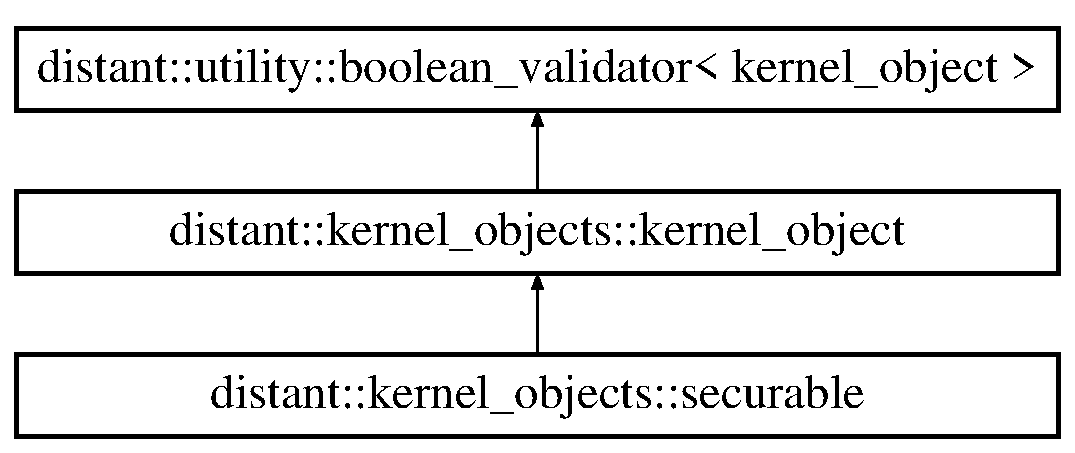
\includegraphics[height=3.000000cm]{classdistant_1_1kernel__objects_1_1securable}
\end{center}
\end{figure}
\subsection*{Public Member Functions}
\begin{DoxyCompactItemize}
\item 
\mbox{\hyperlink{classdistant_1_1kernel__objects_1_1securable_aec5d135541fe36243d7ec121e5bd36fa}{securable}} () noexcept=default
\item 
\mbox{\Hypertarget{classdistant_1_1kernel__objects_1_1securable_a83e1362b9c3c2264603c91d1640a6683}\label{classdistant_1_1kernel__objects_1_1securable_a83e1362b9c3c2264603c91d1640a6683}} 
{\bfseries securable} (\mbox{\hyperlink{classdistant_1_1handle}{distant\+::handle}}$<$ \mbox{\hyperlink{classdistant_1_1kernel__objects_1_1securable}{securable}} $>$ \&\&h)
\item 
\mbox{\Hypertarget{classdistant_1_1kernel__objects_1_1securable_aadf38da104d9aa1b6a66c0a042450d39}\label{classdistant_1_1kernel__objects_1_1securable_aadf38da104d9aa1b6a66c0a042450d39}} 
{\bfseries securable} (\mbox{\hyperlink{classdistant_1_1kernel__objects_1_1securable}{securable}} \&\&tmp) noexcept=default
\item 
\mbox{\Hypertarget{classdistant_1_1kernel__objects_1_1securable_aab9d9f6f85afd6295b031fe18f0ee821}\label{classdistant_1_1kernel__objects_1_1securable_aab9d9f6f85afd6295b031fe18f0ee821}} 
\mbox{\hyperlink{classdistant_1_1kernel__objects_1_1securable}{securable}} \& {\bfseries operator=} (\mbox{\hyperlink{classdistant_1_1kernel__objects_1_1securable}{securable}} \&\&other) noexcept=default
\end{DoxyCompactItemize}
\subsection*{Additional Inherited Members}


\subsection{Constructor \& Destructor Documentation}
\mbox{\Hypertarget{classdistant_1_1kernel__objects_1_1securable_aec5d135541fe36243d7ec121e5bd36fa}\label{classdistant_1_1kernel__objects_1_1securable_aec5d135541fe36243d7ec121e5bd36fa}} 
\index{distant\+::kernel\+\_\+objects\+::securable@{distant\+::kernel\+\_\+objects\+::securable}!securable@{securable}}
\index{securable@{securable}!distant\+::kernel\+\_\+objects\+::securable@{distant\+::kernel\+\_\+objects\+::securable}}
\subsubsection{\texorpdfstring{securable()}{securable()}}
{\footnotesize\ttfamily distant\+::kernel\+\_\+objects\+::securable\+::securable (\begin{DoxyParamCaption}{ }\end{DoxyParamCaption})\hspace{0.3cm}{\ttfamily [default]}, {\ttfamily [noexcept]}}

Windows Object constructors 

The documentation for this class was generated from the following file\+:\begin{DoxyCompactItemize}
\item 
C\+:/\+Users/dinne/source/repos/distant dev/distant dev/include/distant/kernel\+\_\+objects/securable.\+hpp\end{DoxyCompactItemize}

\hypertarget{classdistant_1_1kernel__objects_1_1snapshot}{}\section{distant\+:\+:kernel\+\_\+objects\+:\+:snapshot$<$ Kernel\+Object $>$ Class Template Reference}
\label{classdistant_1_1kernel__objects_1_1snapshot}\index{distant\+::kernel\+\_\+objects\+::snapshot$<$ Kernel\+Object $>$@{distant\+::kernel\+\_\+objects\+::snapshot$<$ Kernel\+Object $>$}}


A snapshot is a read-\/only copy of the current state of one or more of the following lists that reside in system memory\+: processes, threads, modules, and heaps. snapshot is a range modelling \href{http://en.cppreference.com/w/cpp/experimental/ranges/range/InputRange}{\tt Input\+Range} whose elements consist of valid instances of the specified {\itshape Kernel\+Object}.  




{\ttfamily \#include $<$snapshot.\+hpp$>$}

Inheritance diagram for distant\+:\+:kernel\+\_\+objects\+:\+:snapshot$<$ Kernel\+Object $>$\+:\begin{figure}[H]
\begin{center}
\leavevmode
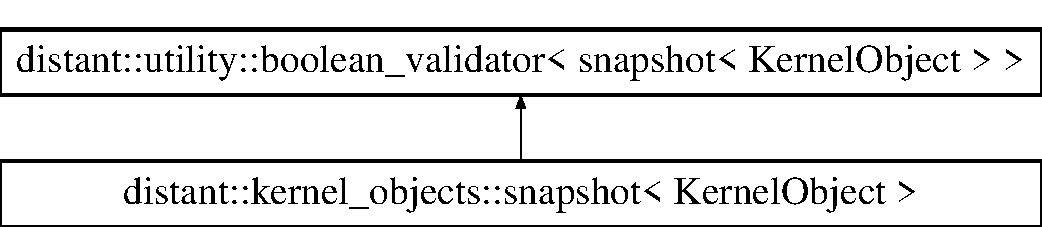
\includegraphics[height=2.000000cm]{classdistant_1_1kernel__objects_1_1snapshot}
\end{center}
\end{figure}
\subsection*{Public Types}
\begin{DoxyCompactItemize}
\item 
\mbox{\Hypertarget{classdistant_1_1kernel__objects_1_1snapshot_adedc8b82516c5fe51aa9a101ed0510db}\label{classdistant_1_1kernel__objects_1_1snapshot_adedc8b82516c5fe51aa9a101ed0510db}} 
using {\bfseries object\+\_\+type} = Kernel\+Object
\item 
\mbox{\Hypertarget{classdistant_1_1kernel__objects_1_1snapshot_a21acc69ce4300aad20f0a6a33aa09e66}\label{classdistant_1_1kernel__objects_1_1snapshot_a21acc69ce4300aad20f0a6a33aa09e66}} 
using {\bfseries handle\+\_\+type} = \mbox{\hyperlink{classdistant_1_1handle}{handle}}$<$ \mbox{\hyperlink{classdistant_1_1kernel__objects_1_1snapshot}{snapshot}} $>$
\item 
\mbox{\Hypertarget{classdistant_1_1kernel__objects_1_1snapshot_ad354c24667f1204e85025da5b45c2354}\label{classdistant_1_1kernel__objects_1_1snapshot_ad354c24667f1204e85025da5b45c2354}} 
using {\bfseries iterator} = \mbox{\hyperlink{classdistant_1_1kernel__objects_1_1snapshot__iterator}{snapshot\+\_\+iterator}}$<$ Kernel\+Object $>$
\item 
\mbox{\Hypertarget{classdistant_1_1kernel__objects_1_1snapshot_ae41a205d6d070f8b50242de623779ce0}\label{classdistant_1_1kernel__objects_1_1snapshot_ae41a205d6d070f8b50242de623779ce0}} 
using {\bfseries const\+\_\+iterator} = \mbox{\hyperlink{classdistant_1_1kernel__objects_1_1snapshot__iterator}{snapshot\+\_\+iterator}}$<$ Kernel\+Object $>$
\end{DoxyCompactItemize}
\subsection*{Public Member Functions}
\begin{DoxyCompactItemize}
\item 
\mbox{\hyperlink{classdistant_1_1kernel__objects_1_1snapshot__iterator}{iterator}} \mbox{\hyperlink{classdistant_1_1kernel__objects_1_1snapshot_a5e9c95fe747a3f4d28dc3d352874770e}{begin}} () const
\begin{DoxyCompactList}\small\item\em Retrieve the start of the snapshot. \end{DoxyCompactList}\item 
\mbox{\hyperlink{classdistant_1_1kernel__objects_1_1snapshot__iterator}{iterator}} \mbox{\hyperlink{classdistant_1_1kernel__objects_1_1snapshot_a4fd564b2c8dda5816fb134688e708924}{end}} () const
\begin{DoxyCompactList}\small\item\em The end of the snapshot. \end{DoxyCompactList}\item 
\mbox{\hyperlink{classdistant_1_1kernel__objects_1_1snapshot__iterator}{iterator}} \mbox{\hyperlink{classdistant_1_1kernel__objects_1_1snapshot_ab23f1b74e2799ece901299d4f69015cc}{begin}} ()
\begin{DoxyCompactList}\small\item\em Retrieve the start of the snapshot. \end{DoxyCompactList}\item 
\mbox{\hyperlink{classdistant_1_1kernel__objects_1_1snapshot__iterator}{iterator}} \mbox{\hyperlink{classdistant_1_1kernel__objects_1_1snapshot_a0ab636ba02b2ec13644a02b00317c4bb}{end}} ()
\begin{DoxyCompactList}\small\item\em The end of the snapshot. \end{DoxyCompactList}\item 
\mbox{\Hypertarget{classdistant_1_1kernel__objects_1_1snapshot_a4f852a80ef0db09296ca25d4af4d1800}\label{classdistant_1_1kernel__objects_1_1snapshot_a4f852a80ef0db09296ca25d4af4d1800}} 
{\footnotesize template$<$template$<$ typename, typename $>$ class Out\+Container$>$ }\\Out\+Container$<$ Kernel\+Object, std\+::allocator$<$ Kernel\+Object $>$ $>$ \mbox{\hyperlink{classdistant_1_1kernel__objects_1_1snapshot_a4f852a80ef0db09296ca25d4af4d1800}{as}} () const
\begin{DoxyCompactList}\small\item\em Store a permanent copy of the snapshot as a container. \end{DoxyCompactList}\item 
{\footnotesize template$<$template$<$ typename, typename $>$ class Out\+Container, typename Predicate $>$ }\\Out\+Container$<$ Kernel\+Object, std\+::allocator$<$ Kernel\+Object $>$ $>$ \mbox{\hyperlink{classdistant_1_1kernel__objects_1_1snapshot_a6e9d7ef5c4273d1dde5fee1055a63b7a}{as}} (Predicate) const
\begin{DoxyCompactList}\small\item\em Store a permanent copy of the snapshot as a container whose elements satisfy the given {\itshape Predicate}. \end{DoxyCompactList}\item 
\mbox{\Hypertarget{classdistant_1_1kernel__objects_1_1snapshot_ac5988aabacb149278b666a9903bbe9c7}\label{classdistant_1_1kernel__objects_1_1snapshot_ac5988aabacb149278b666a9903bbe9c7}} 
\mbox{\hyperlink{classdistant_1_1kernel__objects_1_1snapshot_ac5988aabacb149278b666a9903bbe9c7}{snapshot}} ()
\begin{DoxyCompactList}\small\item\em Default construct a snapshot of all {\itshape Kernel\+Objects} at the current time. \end{DoxyCompactList}\item 
\mbox{\Hypertarget{classdistant_1_1kernel__objects_1_1snapshot_a35c6b486633d03b207ab536771e86b16}\label{classdistant_1_1kernel__objects_1_1snapshot_a35c6b486633d03b207ab536771e86b16}} 
\mbox{\hyperlink{classdistant_1_1kernel__objects_1_1snapshot_a35c6b486633d03b207ab536771e86b16}{snapshot}} (const \mbox{\hyperlink{classdistant_1_1kernel__objects_1_1process}{process}}$<$$>$ \&)
\begin{DoxyCompactList}\small\item\em Construct a snapshot of {\itshape Kernel\+Objects} owned by the given process. \end{DoxyCompactList}\item 
\mbox{\Hypertarget{classdistant_1_1kernel__objects_1_1snapshot_a1a6f5f5e41cb82810a675b5d0b607ba2}\label{classdistant_1_1kernel__objects_1_1snapshot_a1a6f5f5e41cb82810a675b5d0b607ba2}} 
{\footnotesize template$<$template$<$ typename, typename $>$ class Out\+Container$>$ }\\Out\+Container$<$ O, std\+::allocator$<$ O $>$ $>$ {\bfseries as} () const
\item 
\mbox{\Hypertarget{classdistant_1_1kernel__objects_1_1snapshot_aa47a96259e30ef7fd2c495b2d75c18af}\label{classdistant_1_1kernel__objects_1_1snapshot_aa47a96259e30ef7fd2c495b2d75c18af}} 
{\footnotesize template$<$template$<$ typename, typename $>$ class Out\+Container, typename Predicate $>$ }\\Out\+Container$<$ O, std\+::allocator$<$ O $>$ $>$ {\bfseries as} (Predicate predicate) const
\end{DoxyCompactItemize}
\subsection*{Friends}
\begin{DoxyCompactItemize}
\item 
\mbox{\Hypertarget{classdistant_1_1kernel__objects_1_1snapshot_a67171474c4da6cc8efe0c7fafefd2b2d}\label{classdistant_1_1kernel__objects_1_1snapshot_a67171474c4da6cc8efe0c7fafefd2b2d}} 
class {\bfseries iterator}
\end{DoxyCompactItemize}


\subsection{Detailed Description}
\subsubsection*{template$<$typename Kernel\+Object$>$\newline
class distant\+::kernel\+\_\+objects\+::snapshot$<$ Kernel\+Object $>$}

A snapshot is a read-\/only copy of the current state of one or more of the following lists that reside in system memory\+: processes, threads, modules, and heaps. snapshot is a range modelling \href{http://en.cppreference.com/w/cpp/experimental/ranges/range/InputRange}{\tt Input\+Range} whose elements consist of valid instances of the specified {\itshape Kernel\+Object}. 


\begin{DoxyTemplParams}{Template Parameters}
{\em Kernel\+Object} & must be one of the following\+: process, thread, heap, module. \\
\hline
\end{DoxyTemplParams}


\subsection{Member Function Documentation}
\mbox{\Hypertarget{classdistant_1_1kernel__objects_1_1snapshot_a6e9d7ef5c4273d1dde5fee1055a63b7a}\label{classdistant_1_1kernel__objects_1_1snapshot_a6e9d7ef5c4273d1dde5fee1055a63b7a}} 
\index{distant\+::kernel\+\_\+objects\+::snapshot@{distant\+::kernel\+\_\+objects\+::snapshot}!as@{as}}
\index{as@{as}!distant\+::kernel\+\_\+objects\+::snapshot@{distant\+::kernel\+\_\+objects\+::snapshot}}
\subsubsection{\texorpdfstring{as()}{as()}}
{\footnotesize\ttfamily template$<$typename Kernel\+Object$>$ \\
template$<$template$<$ typename, typename $>$ class Out\+Container, typename Predicate $>$ \\
Out\+Container$<$Kernel\+Object, std\+::allocator$<$Kernel\+Object$>$ $>$ \mbox{\hyperlink{classdistant_1_1kernel__objects_1_1snapshot}{distant\+::kernel\+\_\+objects\+::snapshot}}$<$ Kernel\+Object $>$\+::as (\begin{DoxyParamCaption}\item[{Predicate}]{ }\end{DoxyParamCaption}) const}



Store a permanent copy of the snapshot as a container whose elements satisfy the given {\itshape Predicate}. 


\begin{DoxyTemplParams}{Template Parameters}
{\em Predicate} & the {\itshape Predicate} function {\itshape Kernel\+Objects} of the {\itshape Out\+Container} must satisfy. \\
\hline
{\em Out\+Container} & the container in which to store the {\itshape Kernel\+Objects}. \\
\hline
\end{DoxyTemplParams}
\mbox{\Hypertarget{classdistant_1_1kernel__objects_1_1snapshot_a5e9c95fe747a3f4d28dc3d352874770e}\label{classdistant_1_1kernel__objects_1_1snapshot_a5e9c95fe747a3f4d28dc3d352874770e}} 
\index{distant\+::kernel\+\_\+objects\+::snapshot@{distant\+::kernel\+\_\+objects\+::snapshot}!begin@{begin}}
\index{begin@{begin}!distant\+::kernel\+\_\+objects\+::snapshot@{distant\+::kernel\+\_\+objects\+::snapshot}}
\subsubsection{\texorpdfstring{begin()}{begin()}\hspace{0.1cm}{\footnotesize\ttfamily [1/2]}}
{\footnotesize\ttfamily template$<$typename O $>$ \\
\mbox{\hyperlink{classdistant_1_1kernel__objects_1_1snapshot}{snapshot}}$<$ O $>$\+::\mbox{\hyperlink{classdistant_1_1kernel__objects_1_1snapshot__iterator}{iterator}} \mbox{\hyperlink{classdistant_1_1kernel__objects_1_1snapshot}{distant\+::kernel\+\_\+objects\+::snapshot}}$<$ O $>$\+::begin (\begin{DoxyParamCaption}{ }\end{DoxyParamCaption}) const}



Retrieve the start of the snapshot. 

\begin{DoxyReturn}{Returns}
A {\itshape \mbox{\hyperlink{classdistant_1_1kernel__objects_1_1snapshot__iterator}{snapshot\+\_\+iterator}}} pointing to the first element in the snapshot. 
\end{DoxyReturn}
\mbox{\Hypertarget{classdistant_1_1kernel__objects_1_1snapshot_ab23f1b74e2799ece901299d4f69015cc}\label{classdistant_1_1kernel__objects_1_1snapshot_ab23f1b74e2799ece901299d4f69015cc}} 
\index{distant\+::kernel\+\_\+objects\+::snapshot@{distant\+::kernel\+\_\+objects\+::snapshot}!begin@{begin}}
\index{begin@{begin}!distant\+::kernel\+\_\+objects\+::snapshot@{distant\+::kernel\+\_\+objects\+::snapshot}}
\subsubsection{\texorpdfstring{begin()}{begin()}\hspace{0.1cm}{\footnotesize\ttfamily [2/2]}}
{\footnotesize\ttfamily template$<$typename O $>$ \\
\mbox{\hyperlink{classdistant_1_1kernel__objects_1_1snapshot}{snapshot}}$<$ O $>$\+::\mbox{\hyperlink{classdistant_1_1kernel__objects_1_1snapshot__iterator}{iterator}} \mbox{\hyperlink{classdistant_1_1kernel__objects_1_1snapshot}{distant\+::kernel\+\_\+objects\+::snapshot}}$<$ O $>$\+::begin (\begin{DoxyParamCaption}{ }\end{DoxyParamCaption})}



Retrieve the start of the snapshot. 

\begin{DoxyReturn}{Returns}
A {\itshape \mbox{\hyperlink{classdistant_1_1kernel__objects_1_1snapshot__iterator}{snapshot\+\_\+iterator}}} pointing to the first element in the snapshot. 
\end{DoxyReturn}
\mbox{\Hypertarget{classdistant_1_1kernel__objects_1_1snapshot_a4fd564b2c8dda5816fb134688e708924}\label{classdistant_1_1kernel__objects_1_1snapshot_a4fd564b2c8dda5816fb134688e708924}} 
\index{distant\+::kernel\+\_\+objects\+::snapshot@{distant\+::kernel\+\_\+objects\+::snapshot}!end@{end}}
\index{end@{end}!distant\+::kernel\+\_\+objects\+::snapshot@{distant\+::kernel\+\_\+objects\+::snapshot}}
\subsubsection{\texorpdfstring{end()}{end()}\hspace{0.1cm}{\footnotesize\ttfamily [1/2]}}
{\footnotesize\ttfamily template$<$typename O $>$ \\
\mbox{\hyperlink{classdistant_1_1kernel__objects_1_1snapshot}{snapshot}}$<$ O $>$\+::\mbox{\hyperlink{classdistant_1_1kernel__objects_1_1snapshot__iterator}{iterator}} \mbox{\hyperlink{classdistant_1_1kernel__objects_1_1snapshot}{distant\+::kernel\+\_\+objects\+::snapshot}}$<$ O $>$\+::end (\begin{DoxyParamCaption}{ }\end{DoxyParamCaption}) const}



The end of the snapshot. 

\begin{DoxyReturn}{Returns}
a {\itshape \mbox{\hyperlink{classdistant_1_1kernel__objects_1_1snapshot__iterator}{snapshot\+\_\+iterator}}} indicating an element past-\/the-\/end of the snapshot. 
\end{DoxyReturn}
\mbox{\Hypertarget{classdistant_1_1kernel__objects_1_1snapshot_a0ab636ba02b2ec13644a02b00317c4bb}\label{classdistant_1_1kernel__objects_1_1snapshot_a0ab636ba02b2ec13644a02b00317c4bb}} 
\index{distant\+::kernel\+\_\+objects\+::snapshot@{distant\+::kernel\+\_\+objects\+::snapshot}!end@{end}}
\index{end@{end}!distant\+::kernel\+\_\+objects\+::snapshot@{distant\+::kernel\+\_\+objects\+::snapshot}}
\subsubsection{\texorpdfstring{end()}{end()}\hspace{0.1cm}{\footnotesize\ttfamily [2/2]}}
{\footnotesize\ttfamily template$<$typename O $>$ \\
\mbox{\hyperlink{classdistant_1_1kernel__objects_1_1snapshot}{snapshot}}$<$ O $>$\+::\mbox{\hyperlink{classdistant_1_1kernel__objects_1_1snapshot__iterator}{iterator}} \mbox{\hyperlink{classdistant_1_1kernel__objects_1_1snapshot}{distant\+::kernel\+\_\+objects\+::snapshot}}$<$ O $>$\+::end (\begin{DoxyParamCaption}{ }\end{DoxyParamCaption})}



The end of the snapshot. 

\begin{DoxyReturn}{Returns}
a {\itshape \mbox{\hyperlink{classdistant_1_1kernel__objects_1_1snapshot__iterator}{snapshot\+\_\+iterator}}} pointing past-\/the-\/end of the last element in the snapshot. 
\end{DoxyReturn}


The documentation for this class was generated from the following files\+:\begin{DoxyCompactItemize}
\item 
C\+:/\+Users/dinne/source/repos/distant dev/distant dev/include/distant/kernel\+\_\+objects/fwd.\+hpp\item 
C\+:/\+Users/dinne/source/repos/distant dev/distant dev/include/distant/kernel\+\_\+objects/snapshot.\+hpp\item 
C\+:/\+Users/dinne/source/repos/distant dev/distant dev/include/distant/kernel\+\_\+objects/impl/snapshot.\+hxx\end{DoxyCompactItemize}

\hypertarget{structdistant_1_1kernel__objects_1_1detail_1_1snapshot__dispatcher}{}\section{distant\+:\+:kernel\+\_\+objects\+:\+:detail\+:\+:snapshot\+\_\+dispatcher$<$ T $>$ Struct Template Reference}
\label{structdistant_1_1kernel__objects_1_1detail_1_1snapshot__dispatcher}\index{distant\+::kernel\+\_\+objects\+::detail\+::snapshot\+\_\+dispatcher$<$ T $>$@{distant\+::kernel\+\_\+objects\+::detail\+::snapshot\+\_\+dispatcher$<$ T $>$}}


The documentation for this struct was generated from the following file\+:\begin{DoxyCompactItemize}
\item 
C\+:/\+Users/dinne/source/repos/distant dev/distant dev/include/distant/kernel\+\_\+objects/detail/snapshot\+\_\+traits.\+hpp\end{DoxyCompactItemize}

\hypertarget{structdistant_1_1kernel__objects_1_1detail_1_1snapshot__dispatcher_3_01kernel__objects_1_1process_3_01access_01_4_01_4}{}\section{distant\+:\+:kernel\+\_\+objects\+:\+:detail\+:\+:snapshot\+\_\+dispatcher$<$ kernel\+\_\+objects\+:\+:process$<$ access $>$ $>$ Struct Template Reference}
\label{structdistant_1_1kernel__objects_1_1detail_1_1snapshot__dispatcher_3_01kernel__objects_1_1process_3_01access_01_4_01_4}\index{distant\+::kernel\+\_\+objects\+::detail\+::snapshot\+\_\+dispatcher$<$ kernel\+\_\+objects\+::process$<$ access $>$ $>$@{distant\+::kernel\+\_\+objects\+::detail\+::snapshot\+\_\+dispatcher$<$ kernel\+\_\+objects\+::process$<$ access $>$ $>$}}
\subsection*{Public Types}
\begin{DoxyCompactItemize}
\item 
\mbox{\Hypertarget{structdistant_1_1kernel__objects_1_1detail_1_1snapshot__dispatcher_3_01kernel__objects_1_1process_3_01access_01_4_01_4_ac5366d8b356f0022d5035817149c355a}\label{structdistant_1_1kernel__objects_1_1detail_1_1snapshot__dispatcher_3_01kernel__objects_1_1process_3_01access_01_4_01_4_ac5366d8b356f0022d5035817149c355a}} 
using {\bfseries dispatch} = \mbox{\hyperlink{classdistant_1_1detail_1_1process__tag}{distant\+::detail\+::process\+\_\+tag}}
\item 
\mbox{\Hypertarget{structdistant_1_1kernel__objects_1_1detail_1_1snapshot__dispatcher_3_01kernel__objects_1_1process_3_01access_01_4_01_4_a64f7138cf29ff85be19dab0eb6603789}\label{structdistant_1_1kernel__objects_1_1detail_1_1snapshot__dispatcher_3_01kernel__objects_1_1process_3_01access_01_4_01_4_a64f7138cf29ff85be19dab0eb6603789}} 
using {\bfseries entry\+\_\+type} = \mbox{\hyperlink{structboost_1_1winapi_1_1tag_p_r_o_c_e_s_s_e_n_t_r_y32__}{boost\+::winapi\+::\+P\+R\+O\+C\+E\+S\+S\+E\+N\+T\+R\+Y32\+\_\+}}
\end{DoxyCompactItemize}


The documentation for this struct was generated from the following file\+:\begin{DoxyCompactItemize}
\item 
C\+:/\+Users/dinne/source/repos/distant dev/distant dev/include/distant/kernel\+\_\+objects/detail/snapshot\+\_\+traits.\+hpp\end{DoxyCompactItemize}

\hypertarget{structdistant_1_1kernel__objects_1_1detail_1_1snapshot__dispatcher_3_01kernel__objects_1_1process__base_01_4}{}\section{distant\+:\+:kernel\+\_\+objects\+:\+:detail\+:\+:snapshot\+\_\+dispatcher$<$ kernel\+\_\+objects\+:\+:process\+\_\+base $>$ Struct Template Reference}
\label{structdistant_1_1kernel__objects_1_1detail_1_1snapshot__dispatcher_3_01kernel__objects_1_1process__base_01_4}\index{distant\+::kernel\+\_\+objects\+::detail\+::snapshot\+\_\+dispatcher$<$ kernel\+\_\+objects\+::process\+\_\+base $>$@{distant\+::kernel\+\_\+objects\+::detail\+::snapshot\+\_\+dispatcher$<$ kernel\+\_\+objects\+::process\+\_\+base $>$}}
\subsection*{Public Types}
\begin{DoxyCompactItemize}
\item 
\mbox{\Hypertarget{structdistant_1_1kernel__objects_1_1detail_1_1snapshot__dispatcher_3_01kernel__objects_1_1process__base_01_4_acf87f4f154385f3781a1374b9618535f}\label{structdistant_1_1kernel__objects_1_1detail_1_1snapshot__dispatcher_3_01kernel__objects_1_1process__base_01_4_acf87f4f154385f3781a1374b9618535f}} 
using {\bfseries dispatch} = \mbox{\hyperlink{classdistant_1_1detail_1_1process__tag}{distant\+::detail\+::process\+\_\+tag}}
\item 
\mbox{\Hypertarget{structdistant_1_1kernel__objects_1_1detail_1_1snapshot__dispatcher_3_01kernel__objects_1_1process__base_01_4_a8bbf162cfc2b881188438a8f433e8296}\label{structdistant_1_1kernel__objects_1_1detail_1_1snapshot__dispatcher_3_01kernel__objects_1_1process__base_01_4_a8bbf162cfc2b881188438a8f433e8296}} 
using {\bfseries entry\+\_\+type} = \mbox{\hyperlink{structboost_1_1winapi_1_1tag_p_r_o_c_e_s_s_e_n_t_r_y32__}{boost\+::winapi\+::\+P\+R\+O\+C\+E\+S\+S\+E\+N\+T\+R\+Y32\+\_\+}}
\end{DoxyCompactItemize}


The documentation for this struct was generated from the following file\+:\begin{DoxyCompactItemize}
\item 
C\+:/\+Users/dinne/source/repos/distant dev/distant dev/include/distant/kernel\+\_\+objects/detail/snapshot\+\_\+traits.\+hpp\end{DoxyCompactItemize}

\hypertarget{classdistant_1_1kernel__objects_1_1snapshot__iterator}{}\section{distant\+:\+:kernel\+\_\+objects\+:\+:snapshot\+\_\+iterator$<$ Kernel\+Object $>$ Class Template Reference}
\label{classdistant_1_1kernel__objects_1_1snapshot__iterator}\index{distant\+::kernel\+\_\+objects\+::snapshot\+\_\+iterator$<$ Kernel\+Object $>$@{distant\+::kernel\+\_\+objects\+::snapshot\+\_\+iterator$<$ Kernel\+Object $>$}}
Inheritance diagram for distant\+:\+:kernel\+\_\+objects\+:\+:snapshot\+\_\+iterator$<$ Kernel\+Object $>$\+:\begin{figure}[H]
\begin{center}
\leavevmode
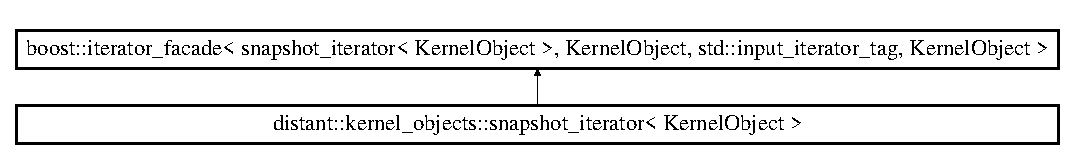
\includegraphics[height=1.707317cm]{classdistant_1_1kernel__objects_1_1snapshot__iterator}
\end{center}
\end{figure}
\subsection*{Public Member Functions}
\begin{DoxyCompactItemize}
\item 
\mbox{\Hypertarget{classdistant_1_1kernel__objects_1_1snapshot__iterator_adc4e283d1e1ea05bddcac342931baef7}\label{classdistant_1_1kernel__objects_1_1snapshot__iterator_adc4e283d1e1ea05bddcac342931baef7}} 
{\bfseries snapshot\+\_\+iterator} (const \mbox{\hyperlink{classdistant_1_1kernel__objects_1_1snapshot}{snapshot\+\_\+type}} \&\mbox{\hyperlink{classdistant_1_1kernel__objects_1_1snapshot}{snapshot}})
\end{DoxyCompactItemize}
\subsection*{Friends}
\begin{DoxyCompactItemize}
\item 
\mbox{\Hypertarget{classdistant_1_1kernel__objects_1_1snapshot__iterator_ac09f73e325921cc50ebcd96bed0f8096}\label{classdistant_1_1kernel__objects_1_1snapshot__iterator_ac09f73e325921cc50ebcd96bed0f8096}} 
class {\bfseries boost\+::iterator\+\_\+core\+\_\+access}
\end{DoxyCompactItemize}


The documentation for this class was generated from the following files\+:\begin{DoxyCompactItemize}
\item 
C\+:/\+Users/dinne/source/repos/distant dev/distant dev/include/distant/kernel\+\_\+objects/snapshot\+\_\+iterator.\+hpp\item 
C\+:/\+Users/dinne/source/repos/distant dev/distant dev/include/distant/kernel\+\_\+objects/impl/snapshot\+\_\+iterator.\+hxx\end{DoxyCompactItemize}

\hypertarget{classdistant_1_1assembly_1_1static__assembler}{}\section{distant\+:\+:assembly\+:\+:static\+\_\+assembler$<$ Size, Instr\+Count $>$ Class Template Reference}
\label{classdistant_1_1assembly_1_1static__assembler}\index{distant\+::assembly\+::static\+\_\+assembler$<$ Size, Instr\+Count $>$@{distant\+::assembly\+::static\+\_\+assembler$<$ Size, Instr\+Count $>$}}
\subsection*{Public Types}
\begin{DoxyCompactItemize}
\item 
\mbox{\Hypertarget{classdistant_1_1assembly_1_1static__assembler_a6844acc5b4275fdfa8e792ccc2c9d752}\label{classdistant_1_1assembly_1_1static__assembler_a6844acc5b4275fdfa8e792ccc2c9d752}} 
using {\bfseries iterator} = \mbox{\hyperlink{classdistant_1_1assembly_1_1static__assembler__iterator}{static\+\_\+assembler\+\_\+iterator}}$<$ Size, Instr\+Count $>$
\item 
\mbox{\Hypertarget{classdistant_1_1assembly_1_1static__assembler_aaa3429d102c44944957fbd42671409b7}\label{classdistant_1_1assembly_1_1static__assembler_aaa3429d102c44944957fbd42671409b7}} 
using {\bfseries const\+\_\+iterator} = \mbox{\hyperlink{classdistant_1_1assembly_1_1static__assembler__iterator}{iterator}}
\item 
\mbox{\Hypertarget{classdistant_1_1assembly_1_1static__assembler_a777c4da52660a04ea2cc8bc498577933}\label{classdistant_1_1assembly_1_1static__assembler_a777c4da52660a04ea2cc8bc498577933}} 
using {\bfseries index} = std\+::size\+\_\+t
\item 
\mbox{\Hypertarget{classdistant_1_1assembly_1_1static__assembler_a14772cbaaa951decb64dcb6b98e33aeb}\label{classdistant_1_1assembly_1_1static__assembler_a14772cbaaa951decb64dcb6b98e33aeb}} 
using {\bfseries opcode\+\_\+length} = std\+::size\+\_\+t
\item 
\mbox{\Hypertarget{classdistant_1_1assembly_1_1static__assembler_afd4e2df1cd2795194c011036327bf595}\label{classdistant_1_1assembly_1_1static__assembler_afd4e2df1cd2795194c011036327bf595}} 
using {\bfseries instruction\+\_\+length} = std\+::size\+\_\+t
\item 
\mbox{\Hypertarget{classdistant_1_1assembly_1_1static__assembler_ab6e0b98d80d6094fce23502f2010ffba}\label{classdistant_1_1assembly_1_1static__assembler_ab6e0b98d80d6094fce23502f2010ffba}} 
using {\bfseries instruction\+\_\+ptr} = std\+::tuple$<$ index, opcode\+\_\+length, instruction\+\_\+length $>$
\end{DoxyCompactItemize}
\subsection*{Public Member Functions}
\begin{DoxyCompactItemize}
\item 
\mbox{\Hypertarget{classdistant_1_1assembly_1_1static__assembler_ada840b6ad572d0d5786826ba9b3531d0}\label{classdistant_1_1assembly_1_1static__assembler_ada840b6ad572d0d5786826ba9b3531d0}} 
constexpr \mbox{\hyperlink{classdistant_1_1assembly_1_1static__assembler__iterator}{iterator}} {\bfseries begin} () const
\item 
\mbox{\Hypertarget{classdistant_1_1assembly_1_1static__assembler_a0354fc20fba2022df2a0346698fe7605}\label{classdistant_1_1assembly_1_1static__assembler_a0354fc20fba2022df2a0346698fe7605}} 
constexpr \mbox{\hyperlink{classdistant_1_1assembly_1_1static__assembler__iterator}{iterator}} {\bfseries end} () const
\item 
\mbox{\Hypertarget{classdistant_1_1assembly_1_1static__assembler_a26df9749ddfd9040b7def347ba50435c}\label{classdistant_1_1assembly_1_1static__assembler_a26df9749ddfd9040b7def347ba50435c}} 
constexpr {\bfseries static\+\_\+assembler} (const std\+::array$<$ byte, Size $>$ \&bytes, const std\+::array$<$ instruction\+\_\+ptr, Instr\+Count $>$ \&instruction\+\_\+ptrs) noexcept
\end{DoxyCompactItemize}
\subsection*{Friends}
\begin{DoxyCompactItemize}
\item 
\mbox{\Hypertarget{classdistant_1_1assembly_1_1static__assembler_a9604961da7981a7989f42842bd1273b8}\label{classdistant_1_1assembly_1_1static__assembler_a9604961da7981a7989f42842bd1273b8}} 
{\footnotesize template$<$std\+::size\+\_\+t S, std\+::size\+\_\+t IC$>$ }\\class {\bfseries static\+\_\+instruction}
\item 
\mbox{\Hypertarget{classdistant_1_1assembly_1_1static__assembler_a4dac94e37604f6ccf8734bdc7c336ea9}\label{classdistant_1_1assembly_1_1static__assembler_a4dac94e37604f6ccf8734bdc7c336ea9}} 
{\footnotesize template$<$std\+::size\+\_\+t S, std\+::size\+\_\+t IC$>$ }\\class {\bfseries static\+\_\+assembler\+\_\+iterator}
\item 
\mbox{\Hypertarget{classdistant_1_1assembly_1_1static__assembler_a340e6bcde814c6003c7bba5a0a9da5c3}\label{classdistant_1_1assembly_1_1static__assembler_a340e6bcde814c6003c7bba5a0a9da5c3}} 
{\footnotesize template$<$std\+::size\+\_\+t First, std\+::size\+\_\+t First\+Count, std\+::size\+\_\+t Second$>$ }\\constexpr \mbox{\hyperlink{classdistant_1_1assembly_1_1static__assembler}{static\+\_\+assembler}}$<$ First+Second, First\+Count+1 $>$ {\bfseries operator+} (const \mbox{\hyperlink{classdistant_1_1assembly_1_1static__assembler}{static\+\_\+assembler}}$<$ First, First\+Count $>$ \&first, const \mbox{\hyperlink{classdistant_1_1assembly_1_1static__assembler}{static\+\_\+assembler}}$<$ Second, 1 $>$ \&second) noexcept
\end{DoxyCompactItemize}


The documentation for this class was generated from the following files\+:\begin{DoxyCompactItemize}
\item 
C\+:/\+Users/dinne/source/repos/distant dev/distant dev/include/distant/assembly/static\+\_\+assembler.\+hpp\item 
C\+:/\+Users/dinne/source/repos/distant dev/distant dev/include/distant/assembly/impl/static\+\_\+assembler.\+hxx\end{DoxyCompactItemize}

\hypertarget{classdistant_1_1assembly_1_1static__assembler__iterator}{}\section{distant\+:\+:assembly\+:\+:static\+\_\+assembler\+\_\+iterator$<$ Assembler\+Size, Instr\+Count $>$ Class Template Reference}
\label{classdistant_1_1assembly_1_1static__assembler__iterator}\index{distant\+::assembly\+::static\+\_\+assembler\+\_\+iterator$<$ Assembler\+Size, Instr\+Count $>$@{distant\+::assembly\+::static\+\_\+assembler\+\_\+iterator$<$ Assembler\+Size, Instr\+Count $>$}}
Inheritance diagram for distant\+:\+:assembly\+:\+:static\+\_\+assembler\+\_\+iterator$<$ Assembler\+Size, Instr\+Count $>$\+:\begin{figure}[H]
\begin{center}
\leavevmode
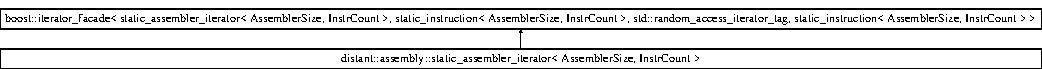
\includegraphics[height=0.916530cm]{classdistant_1_1assembly_1_1static__assembler__iterator}
\end{center}
\end{figure}
\subsection*{Public Member Functions}
\begin{DoxyCompactItemize}
\item 
\mbox{\Hypertarget{classdistant_1_1assembly_1_1static__assembler__iterator_a62f897d79152940b480de52bbeeed76e}\label{classdistant_1_1assembly_1_1static__assembler__iterator_a62f897d79152940b480de52bbeeed76e}} 
constexpr {\bfseries static\+\_\+assembler\+\_\+iterator} (const \mbox{\hyperlink{classdistant_1_1assembly_1_1static__assembler}{static\+\_\+assembler}}$<$ Assembler\+Size, Instr\+Count $>$ \&assembler, std\+::size\+\_\+t index) noexcept
\end{DoxyCompactItemize}
\subsection*{Friends}
\begin{DoxyCompactItemize}
\item 
\mbox{\Hypertarget{classdistant_1_1assembly_1_1static__assembler__iterator_ac09f73e325921cc50ebcd96bed0f8096}\label{classdistant_1_1assembly_1_1static__assembler__iterator_ac09f73e325921cc50ebcd96bed0f8096}} 
class {\bfseries boost\+::iterator\+\_\+core\+\_\+access}
\item 
\mbox{\Hypertarget{classdistant_1_1assembly_1_1static__assembler__iterator_a4dac94e37604f6ccf8734bdc7c336ea9}\label{classdistant_1_1assembly_1_1static__assembler__iterator_a4dac94e37604f6ccf8734bdc7c336ea9}} 
{\footnotesize template$<$std\+::size\+\_\+t S, std\+::size\+\_\+t C$>$ }\\class {\bfseries static\+\_\+assembler\+\_\+iterator}
\end{DoxyCompactItemize}


The documentation for this class was generated from the following files\+:\begin{DoxyCompactItemize}
\item 
C\+:/\+Users/dinne/source/repos/distant dev/distant dev/include/distant/assembly/static\+\_\+assembler\+\_\+iterator.\+hpp\item 
C\+:/\+Users/dinne/source/repos/distant dev/distant dev/include/distant/assembly/impl/static\+\_\+assembler\+\_\+iterator.\+hxx\end{DoxyCompactItemize}

\hypertarget{classdistant_1_1utility_1_1static__downcast}{}\section{distant\+:\+:utility\+:\+:static\+\_\+downcast$<$ derived $>$ Class Template Reference}
\label{classdistant_1_1utility_1_1static__downcast}\index{distant\+::utility\+::static\+\_\+downcast$<$ derived $>$@{distant\+::utility\+::static\+\_\+downcast$<$ derived $>$}}
\subsection*{Public Member Functions}
\begin{DoxyCompactItemize}
\item 
\mbox{\Hypertarget{classdistant_1_1utility_1_1static__downcast_aa6837097d259a39129fab430e0fb9f40}\label{classdistant_1_1utility_1_1static__downcast_aa6837097d259a39129fab430e0fb9f40}} 
const derived $\ast$ {\bfseries self} () const
\item 
\mbox{\Hypertarget{classdistant_1_1utility_1_1static__downcast_a3178f691b633ebaabefb87a221bace63}\label{classdistant_1_1utility_1_1static__downcast_a3178f691b633ebaabefb87a221bace63}} 
derived $\ast$ {\bfseries self} ()
\end{DoxyCompactItemize}


The documentation for this class was generated from the following file\+:\begin{DoxyCompactItemize}
\item 
C\+:/\+Users/dinne/source/repos/distant dev/distant dev/include/distant/utility/static\+\_\+downcast.\+hpp\end{DoxyCompactItemize}

\hypertarget{classdistant_1_1assembly_1_1static__instruction}{}\section{distant\+:\+:assembly\+:\+:static\+\_\+instruction Class Reference}
\label{classdistant_1_1assembly_1_1static__instruction}\index{distant\+::assembly\+::static\+\_\+instruction@{distant\+::assembly\+::static\+\_\+instruction}}
\subsection*{Public Member Functions}
\begin{DoxyCompactItemize}
\item 
\mbox{\Hypertarget{classdistant_1_1assembly_1_1static__instruction_a66479e12ac3dcceeb3fb1460a96e9c70}\label{classdistant_1_1assembly_1_1static__instruction_a66479e12ac3dcceeb3fb1460a96e9c70}} 
constexpr std\+::size\+\_\+t {\bfseries size} () const noexcept
\end{DoxyCompactItemize}


The documentation for this class was generated from the following file\+:\begin{DoxyCompactItemize}
\item 
C\+:/\+Users/dinne/source/repos/distant dev/distant dev/include/distant/assembly/static\+\_\+instruction.\+hpp\end{DoxyCompactItemize}

\hypertarget{classdistant_1_1memory_1_1static__instruction}{}\section{distant\+:\+:memory\+:\+:static\+\_\+instruction$<$ S, C $>$ Class Template Reference}
\label{classdistant_1_1memory_1_1static__instruction}\index{distant\+::memory\+::static\+\_\+instruction$<$ S, C $>$@{distant\+::memory\+::static\+\_\+instruction$<$ S, C $>$}}


The documentation for this class was generated from the following file\+:\begin{DoxyCompactItemize}
\item 
C\+:/\+Users/dinne/source/repos/distant dev/distant dev/include/distant/detail/to\+\_\+string.\+hpp\end{DoxyCompactItemize}

\hypertarget{structdistant_1_1memory_1_1x86__calling__conventions_1_1stdcall}{}\section{distant\+:\+:memory\+:\+:x86\+\_\+calling\+\_\+conventions\+:\+:stdcall Struct Reference}
\label{structdistant_1_1memory_1_1x86__calling__conventions_1_1stdcall}\index{distant\+::memory\+::x86\+\_\+calling\+\_\+conventions\+::stdcall@{distant\+::memory\+::x86\+\_\+calling\+\_\+conventions\+::stdcall}}


The documentation for this struct was generated from the following file\+:\begin{DoxyCompactItemize}
\item 
C\+:/\+Users/dinne/source/repos/distant dev/distant dev/include/distant/memory/x86\+\_\+calling\+\_\+conventions.\+hpp\end{DoxyCompactItemize}

\hypertarget{structboost_1_1winapi_1_1tag_p_r_o_c_e_s_s_e_n_t_r_y32__}{}\section{boost\+:\+:winapi\+:\+:tag\+P\+R\+O\+C\+E\+S\+S\+E\+N\+T\+R\+Y32\+\_\+ Struct Reference}
\label{structboost_1_1winapi_1_1tag_p_r_o_c_e_s_s_e_n_t_r_y32__}\index{boost\+::winapi\+::tag\+P\+R\+O\+C\+E\+S\+S\+E\+N\+T\+R\+Y32\+\_\+@{boost\+::winapi\+::tag\+P\+R\+O\+C\+E\+S\+S\+E\+N\+T\+R\+Y32\+\_\+}}
\subsection*{Public Attributes}
\begin{DoxyCompactItemize}
\item 
\mbox{\Hypertarget{structboost_1_1winapi_1_1tag_p_r_o_c_e_s_s_e_n_t_r_y32___aa1302d8e2e28bbd50ef0f60ed53a8652}\label{structboost_1_1winapi_1_1tag_p_r_o_c_e_s_s_e_n_t_r_y32___aa1302d8e2e28bbd50ef0f60ed53a8652}} 
D\+W\+O\+R\+D\+\_\+ {\bfseries dw\+Size}
\item 
\mbox{\Hypertarget{structboost_1_1winapi_1_1tag_p_r_o_c_e_s_s_e_n_t_r_y32___a498cc39b1afbde0011c5a2956596bf93}\label{structboost_1_1winapi_1_1tag_p_r_o_c_e_s_s_e_n_t_r_y32___a498cc39b1afbde0011c5a2956596bf93}} 
D\+W\+O\+R\+D\+\_\+ {\bfseries cnt\+Usage}
\item 
\mbox{\Hypertarget{structboost_1_1winapi_1_1tag_p_r_o_c_e_s_s_e_n_t_r_y32___a6b92a9740a4b73d85cc12e5b3056a57e}\label{structboost_1_1winapi_1_1tag_p_r_o_c_e_s_s_e_n_t_r_y32___a6b92a9740a4b73d85cc12e5b3056a57e}} 
D\+W\+O\+R\+D\+\_\+ {\bfseries th32\+Process\+ID}
\item 
\mbox{\Hypertarget{structboost_1_1winapi_1_1tag_p_r_o_c_e_s_s_e_n_t_r_y32___a9d20048d3ac6eafc33d3dd3919fe86ea}\label{structboost_1_1winapi_1_1tag_p_r_o_c_e_s_s_e_n_t_r_y32___a9d20048d3ac6eafc33d3dd3919fe86ea}} 
U\+L\+O\+N\+G\+\_\+\+P\+T\+R\+\_\+ {\bfseries th32\+Default\+Heap\+ID}
\item 
\mbox{\Hypertarget{structboost_1_1winapi_1_1tag_p_r_o_c_e_s_s_e_n_t_r_y32___ad1fc79a06d9b3a80cf23e106ec5f3997}\label{structboost_1_1winapi_1_1tag_p_r_o_c_e_s_s_e_n_t_r_y32___ad1fc79a06d9b3a80cf23e106ec5f3997}} 
D\+W\+O\+R\+D\+\_\+ {\bfseries th32\+Module\+ID}
\item 
\mbox{\Hypertarget{structboost_1_1winapi_1_1tag_p_r_o_c_e_s_s_e_n_t_r_y32___a9dcff6a0c959b32be469650601b976c7}\label{structboost_1_1winapi_1_1tag_p_r_o_c_e_s_s_e_n_t_r_y32___a9dcff6a0c959b32be469650601b976c7}} 
D\+W\+O\+R\+D\+\_\+ {\bfseries cnt\+Threads}
\item 
\mbox{\Hypertarget{structboost_1_1winapi_1_1tag_p_r_o_c_e_s_s_e_n_t_r_y32___ad43b5f29ad60f685f26b3d8c0021784a}\label{structboost_1_1winapi_1_1tag_p_r_o_c_e_s_s_e_n_t_r_y32___ad43b5f29ad60f685f26b3d8c0021784a}} 
D\+W\+O\+R\+D\+\_\+ {\bfseries th32\+Parent\+Process\+ID}
\item 
\mbox{\Hypertarget{structboost_1_1winapi_1_1tag_p_r_o_c_e_s_s_e_n_t_r_y32___a1a565e99cc91271290af89e00d01e804}\label{structboost_1_1winapi_1_1tag_p_r_o_c_e_s_s_e_n_t_r_y32___a1a565e99cc91271290af89e00d01e804}} 
L\+O\+N\+G\+\_\+ {\bfseries pc\+Pri\+Class\+Base}
\item 
\mbox{\Hypertarget{structboost_1_1winapi_1_1tag_p_r_o_c_e_s_s_e_n_t_r_y32___afa52672c60b3c165097e9f211e2e81f5}\label{structboost_1_1winapi_1_1tag_p_r_o_c_e_s_s_e_n_t_r_y32___afa52672c60b3c165097e9f211e2e81f5}} 
D\+W\+O\+R\+D\+\_\+ {\bfseries dw\+Flags}
\item 
\mbox{\Hypertarget{structboost_1_1winapi_1_1tag_p_r_o_c_e_s_s_e_n_t_r_y32___a4d35f492f27d02b266685b7ef559408a}\label{structboost_1_1winapi_1_1tag_p_r_o_c_e_s_s_e_n_t_r_y32___a4d35f492f27d02b266685b7ef559408a}} 
C\+H\+A\+R\+\_\+ {\bfseries sz\+Exe\+File} \mbox{[}boost\+::winapi\+::max\+\_\+path\mbox{]}
\end{DoxyCompactItemize}


The documentation for this struct was generated from the following file\+:\begin{DoxyCompactItemize}
\item 
C\+:/\+Users/dinne/source/repos/distant dev/distant dev/include/distant/support/winapi/toolhelp32.\+hpp\end{DoxyCompactItemize}

\hypertarget{structboost_1_1winapi_1_1tag_p_r_o_c_e_s_s_e_n_t_r_y32_w__}{}\section{boost\+:\+:winapi\+:\+:tag\+P\+R\+O\+C\+E\+S\+S\+E\+N\+T\+R\+Y32\+W\+\_\+ Struct Reference}
\label{structboost_1_1winapi_1_1tag_p_r_o_c_e_s_s_e_n_t_r_y32_w__}\index{boost\+::winapi\+::tag\+P\+R\+O\+C\+E\+S\+S\+E\+N\+T\+R\+Y32\+W\+\_\+@{boost\+::winapi\+::tag\+P\+R\+O\+C\+E\+S\+S\+E\+N\+T\+R\+Y32\+W\+\_\+}}
\subsection*{Public Attributes}
\begin{DoxyCompactItemize}
\item 
\mbox{\Hypertarget{structboost_1_1winapi_1_1tag_p_r_o_c_e_s_s_e_n_t_r_y32_w___a7395a33f264c05be95c5520abfa27a7f}\label{structboost_1_1winapi_1_1tag_p_r_o_c_e_s_s_e_n_t_r_y32_w___a7395a33f264c05be95c5520abfa27a7f}} 
D\+W\+O\+R\+D\+\_\+ {\bfseries dw\+Size}
\item 
\mbox{\Hypertarget{structboost_1_1winapi_1_1tag_p_r_o_c_e_s_s_e_n_t_r_y32_w___ab36819d475e21b6f957a205e87043078}\label{structboost_1_1winapi_1_1tag_p_r_o_c_e_s_s_e_n_t_r_y32_w___ab36819d475e21b6f957a205e87043078}} 
D\+W\+O\+R\+D\+\_\+ {\bfseries cnt\+Usage}
\item 
\mbox{\Hypertarget{structboost_1_1winapi_1_1tag_p_r_o_c_e_s_s_e_n_t_r_y32_w___a27a95d97a2dfb5cff70e6b792832af99}\label{structboost_1_1winapi_1_1tag_p_r_o_c_e_s_s_e_n_t_r_y32_w___a27a95d97a2dfb5cff70e6b792832af99}} 
D\+W\+O\+R\+D\+\_\+ {\bfseries th32\+Process\+ID}
\item 
\mbox{\Hypertarget{structboost_1_1winapi_1_1tag_p_r_o_c_e_s_s_e_n_t_r_y32_w___a73542c5eef34f36065323cd997c0ee40}\label{structboost_1_1winapi_1_1tag_p_r_o_c_e_s_s_e_n_t_r_y32_w___a73542c5eef34f36065323cd997c0ee40}} 
U\+L\+O\+N\+G\+\_\+\+P\+T\+R\+\_\+ {\bfseries th32\+Default\+Heap\+ID}
\item 
\mbox{\Hypertarget{structboost_1_1winapi_1_1tag_p_r_o_c_e_s_s_e_n_t_r_y32_w___a185f2b842e9ccf687fbd74a6b6d2fb2d}\label{structboost_1_1winapi_1_1tag_p_r_o_c_e_s_s_e_n_t_r_y32_w___a185f2b842e9ccf687fbd74a6b6d2fb2d}} 
D\+W\+O\+R\+D\+\_\+ {\bfseries th32\+Module\+ID}
\item 
\mbox{\Hypertarget{structboost_1_1winapi_1_1tag_p_r_o_c_e_s_s_e_n_t_r_y32_w___ac4b75ac7da97185f44fdaa0305456ec7}\label{structboost_1_1winapi_1_1tag_p_r_o_c_e_s_s_e_n_t_r_y32_w___ac4b75ac7da97185f44fdaa0305456ec7}} 
D\+W\+O\+R\+D\+\_\+ {\bfseries cnt\+Threads}
\item 
\mbox{\Hypertarget{structboost_1_1winapi_1_1tag_p_r_o_c_e_s_s_e_n_t_r_y32_w___af2dfa5c4dee07d7f0b1f1e8ebd1657eb}\label{structboost_1_1winapi_1_1tag_p_r_o_c_e_s_s_e_n_t_r_y32_w___af2dfa5c4dee07d7f0b1f1e8ebd1657eb}} 
D\+W\+O\+R\+D\+\_\+ {\bfseries th32\+Parent\+Process\+ID}
\item 
\mbox{\Hypertarget{structboost_1_1winapi_1_1tag_p_r_o_c_e_s_s_e_n_t_r_y32_w___a9aa2e403d8ff37dcd01e345211d345a6}\label{structboost_1_1winapi_1_1tag_p_r_o_c_e_s_s_e_n_t_r_y32_w___a9aa2e403d8ff37dcd01e345211d345a6}} 
L\+O\+N\+G\+\_\+ {\bfseries pc\+Pri\+Class\+Base}
\item 
\mbox{\Hypertarget{structboost_1_1winapi_1_1tag_p_r_o_c_e_s_s_e_n_t_r_y32_w___a455ca1e6fd2198652c8db083f7166000}\label{structboost_1_1winapi_1_1tag_p_r_o_c_e_s_s_e_n_t_r_y32_w___a455ca1e6fd2198652c8db083f7166000}} 
D\+W\+O\+R\+D\+\_\+ {\bfseries dw\+Flags}
\item 
\mbox{\Hypertarget{structboost_1_1winapi_1_1tag_p_r_o_c_e_s_s_e_n_t_r_y32_w___a396dfe264f873bf19f13ea0a6378a133}\label{structboost_1_1winapi_1_1tag_p_r_o_c_e_s_s_e_n_t_r_y32_w___a396dfe264f873bf19f13ea0a6378a133}} 
W\+C\+H\+A\+R\+\_\+ {\bfseries sz\+Exe\+File} \mbox{[}M\+A\+X\+\_\+\+P\+A\+T\+H\+\_\+\mbox{]}
\end{DoxyCompactItemize}


The documentation for this struct was generated from the following file\+:\begin{DoxyCompactItemize}
\item 
C\+:/\+Users/dinne/source/repos/distant dev/distant dev/include/distant/support/winapi/toolhelp32.\+hpp\end{DoxyCompactItemize}

\hypertarget{structdistant_1_1memory_1_1x86__calling__conventions_1_1thiscall}{}\section{distant\+:\+:memory\+:\+:x86\+\_\+calling\+\_\+conventions\+:\+:thiscall Struct Reference}
\label{structdistant_1_1memory_1_1x86__calling__conventions_1_1thiscall}\index{distant\+::memory\+::x86\+\_\+calling\+\_\+conventions\+::thiscall@{distant\+::memory\+::x86\+\_\+calling\+\_\+conventions\+::thiscall}}


The documentation for this struct was generated from the following file\+:\begin{DoxyCompactItemize}
\item 
C\+:/\+Users/dinne/source/repos/distant dev/distant dev/include/distant/memory/x86\+\_\+calling\+\_\+conventions.\+hpp\end{DoxyCompactItemize}

\hypertarget{classdistant_1_1kernel__objects_1_1thread}{}\section{distant\+:\+:kernel\+\_\+objects\+:\+:thread Class Reference}
\label{classdistant_1_1kernel__objects_1_1thread}\index{distant\+::kernel\+\_\+objects\+::thread@{distant\+::kernel\+\_\+objects\+::thread}}
\subsection*{Public Member Functions}
\begin{DoxyCompactItemize}
\item 
\mbox{\Hypertarget{classdistant_1_1kernel__objects_1_1thread_a512cd30df2cd62136b004c71b559b870}\label{classdistant_1_1kernel__objects_1_1thread_a512cd30df2cd62136b004c71b559b870}} 
void {\bfseries join} ()
\item 
\mbox{\Hypertarget{classdistant_1_1kernel__objects_1_1thread_a5831cdd5ad10a869e419d80638a14352}\label{classdistant_1_1kernel__objects_1_1thread_a5831cdd5ad10a869e419d80638a14352}} 
void {\bfseries detach} ()
\item 
\mbox{\Hypertarget{classdistant_1_1kernel__objects_1_1thread_a48906753faf5873948c6862bcee13057}\label{classdistant_1_1kernel__objects_1_1thread_a48906753faf5873948c6862bcee13057}} 
void {\bfseries swap} (\mbox{\hyperlink{classdistant_1_1kernel__objects_1_1thread}{thread}} \&other) noexcept
\item 
\mbox{\Hypertarget{classdistant_1_1kernel__objects_1_1thread_ad65a1b00c3aa79c504e328afc9673684}\label{classdistant_1_1kernel__objects_1_1thread_ad65a1b00c3aa79c504e328afc9673684}} 
unsigned int {\bfseries id} () const noexcept
\item 
\mbox{\Hypertarget{classdistant_1_1kernel__objects_1_1thread_a8acda3802aea3811cadb932b7b59e0da}\label{classdistant_1_1kernel__objects_1_1thread_a8acda3802aea3811cadb932b7b59e0da}} 
bool {\bfseries joinable} () const noexcept
\item 
\mbox{\Hypertarget{classdistant_1_1kernel__objects_1_1thread_a528e3ad13c927f14ca156b9b502387ef}\label{classdistant_1_1kernel__objects_1_1thread_a528e3ad13c927f14ca156b9b502387ef}} 
const \mbox{\hyperlink{classdistant_1_1handle}{distant\+::handle}}$<$ \mbox{\hyperlink{classdistant_1_1kernel__objects_1_1thread}{thread}} $>$ \& {\bfseries handle} () const noexcept
\item 
\mbox{\Hypertarget{classdistant_1_1kernel__objects_1_1thread_ae078a839ced841194bd200c58a0e1dba}\label{classdistant_1_1kernel__objects_1_1thread_ae078a839ced841194bd200c58a0e1dba}} 
{\footnotesize template$<$typename Fn , typename... Args$>$ }\\{\bfseries thread} (const \mbox{\hyperlink{classdistant_1_1kernel__objects_1_1process}{process}}$<$ required\+\_\+access $>$ \&, \mbox{\hyperlink{classdistant_1_1memory_1_1function}{function}}$<$ int $>$, Args \&\&... args)
\item 
\mbox{\Hypertarget{classdistant_1_1kernel__objects_1_1thread_a5fddb325cc8c97f82f19f61cd7faa28a}\label{classdistant_1_1kernel__objects_1_1thread_a5fddb325cc8c97f82f19f61cd7faa28a}} 
{\bfseries thread} (\mbox{\hyperlink{classdistant_1_1kernel__objects_1_1thread}{thread}} \&\&other) noexcept
\item 
\mbox{\Hypertarget{classdistant_1_1kernel__objects_1_1thread_a2cd0031da63fcdbd03748cc53d19bbf2}\label{classdistant_1_1kernel__objects_1_1thread_a2cd0031da63fcdbd03748cc53d19bbf2}} 
\mbox{\hyperlink{classdistant_1_1kernel__objects_1_1thread}{thread}} \& {\bfseries operator=} (\mbox{\hyperlink{classdistant_1_1kernel__objects_1_1thread}{thread}} \&\&other) noexcept
\item 
\mbox{\Hypertarget{classdistant_1_1kernel__objects_1_1thread_a970e7208d4c29b628f72cfe5b3799900}\label{classdistant_1_1kernel__objects_1_1thread_a970e7208d4c29b628f72cfe5b3799900}} 
{\bfseries thread} (const \mbox{\hyperlink{classdistant_1_1kernel__objects_1_1thread}{thread}} \&)=delete
\item 
\mbox{\Hypertarget{classdistant_1_1kernel__objects_1_1thread_acefab527ab136157070420f7f0ef0ab6}\label{classdistant_1_1kernel__objects_1_1thread_acefab527ab136157070420f7f0ef0ab6}} 
\mbox{\hyperlink{classdistant_1_1kernel__objects_1_1thread}{thread}} \& {\bfseries operator=} (const \mbox{\hyperlink{classdistant_1_1kernel__objects_1_1thread}{thread}} \&)=delete
\end{DoxyCompactItemize}
\subsection*{Static Public Member Functions}
\begin{DoxyCompactItemize}
\item 
\mbox{\Hypertarget{classdistant_1_1kernel__objects_1_1thread_a1f51ac51c4c9a7129b7226dc6578a5c5}\label{classdistant_1_1kernel__objects_1_1thread_a1f51ac51c4c9a7129b7226dc6578a5c5}} 
static unsigned int {\bfseries hardware\+\_\+concurrency} () noexcept
\end{DoxyCompactItemize}
\subsection*{Static Public Attributes}
\begin{DoxyCompactItemize}
\item 
\mbox{\Hypertarget{classdistant_1_1kernel__objects_1_1thread_a74d71ef6367e7dbfc14edc3ff32c3a4e}\label{classdistant_1_1kernel__objects_1_1thread_a74d71ef6367e7dbfc14edc3ff32c3a4e}} 
static constexpr auto {\bfseries required\+\_\+access} = process\+\_\+rights\+::create\+\_\+thread $\vert$ process\+\_\+rights\+::query\+\_\+information $\vert$ vm\+\_\+rw\+\_\+op
\end{DoxyCompactItemize}


The documentation for this class was generated from the following files\+:\begin{DoxyCompactItemize}
\item 
C\+:/\+Users/dinne/source/repos/distant dev/distant dev/include/distant/kernel\+\_\+objects/thread.\+hpp\item 
C\+:/\+Users/dinne/source/repos/distant dev/distant dev/include/distant/kernel\+\_\+objects/impl/thread.\+hxx\end{DoxyCompactItemize}

\hypertarget{classdistant_1_1detail_1_1thread__tag}{}\section{distant\+:\+:detail\+:\+:thread\+\_\+tag Class Reference}
\label{classdistant_1_1detail_1_1thread__tag}\index{distant\+::detail\+::thread\+\_\+tag@{distant\+::detail\+::thread\+\_\+tag}}


The documentation for this class was generated from the following file\+:\begin{DoxyCompactItemize}
\item 
C\+:/\+Users/dinne/source/repos/distant dev/distant dev/include/distant/detail/tags.\+hpp\end{DoxyCompactItemize}

\hypertarget{classdistant_1_1detail_1_1attorney_1_1to__handle}{}\section{distant\+:\+:detail\+:\+:attorney\+:\+:to\+\_\+handle$<$ Accessor $>$ Class Template Reference}
\label{classdistant_1_1detail_1_1attorney_1_1to__handle}\index{distant\+::detail\+::attorney\+::to\+\_\+handle$<$ Accessor $>$@{distant\+::detail\+::attorney\+::to\+\_\+handle$<$ Accessor $>$}}


The documentation for this class was generated from the following file\+:\begin{DoxyCompactItemize}
\item 
C\+:/\+Users/dinne/source/repos/distant dev/distant dev/include/distant/detail/attorney.\+hpp\end{DoxyCompactItemize}

\hypertarget{classdistant_1_1detail_1_1token__tag}{}\section{distant\+:\+:detail\+:\+:token\+\_\+tag Class Reference}
\label{classdistant_1_1detail_1_1token__tag}\index{distant\+::detail\+::token\+\_\+tag@{distant\+::detail\+::token\+\_\+tag}}


The documentation for this class was generated from the following file\+:\begin{DoxyCompactItemize}
\item 
C\+:/\+Users/dinne/source/repos/distant dev/distant dev/include/distant/detail/tags.\+hpp\end{DoxyCompactItemize}

\hypertarget{structstd_1_1tuple__size_3_01distant_1_1utility_1_1meta_1_1map_3_01_key_00_01_value_00_01_size_01_4_01_4}{}\section{std\+:\+:tuple\+\_\+size$<$ distant\+:\+:utility\+:\+:meta\+:\+:map$<$ Key, Value, Size $>$ $>$ Struct Template Reference}
\label{structstd_1_1tuple__size_3_01distant_1_1utility_1_1meta_1_1map_3_01_key_00_01_value_00_01_size_01_4_01_4}\index{std\+::tuple\+\_\+size$<$ distant\+::utility\+::meta\+::map$<$ Key, Value, Size $>$ $>$@{std\+::tuple\+\_\+size$<$ distant\+::utility\+::meta\+::map$<$ Key, Value, Size $>$ $>$}}
\subsection*{Static Public Attributes}
\begin{DoxyCompactItemize}
\item 
\mbox{\Hypertarget{structstd_1_1tuple__size_3_01distant_1_1utility_1_1meta_1_1map_3_01_key_00_01_value_00_01_size_01_4_01_4_a341d096836568e90d3a65d0c623dadb5}\label{structstd_1_1tuple__size_3_01distant_1_1utility_1_1meta_1_1map_3_01_key_00_01_value_00_01_size_01_4_01_4_a341d096836568e90d3a65d0c623dadb5}} 
static constexpr auto {\bfseries value} = Size
\end{DoxyCompactItemize}


The documentation for this struct was generated from the following file\+:\begin{DoxyCompactItemize}
\item 
C\+:/\+Users/dinne/source/repos/distant dev/distant dev/include/distant/utility/meta/map.\+hpp\end{DoxyCompactItemize}

\hypertarget{structdistant_1_1memory_1_1x86__calling__conventions_1_1vectorcall}{}\section{distant\+:\+:memory\+:\+:x86\+\_\+calling\+\_\+conventions\+:\+:vectorcall Struct Reference}
\label{structdistant_1_1memory_1_1x86__calling__conventions_1_1vectorcall}\index{distant\+::memory\+::x86\+\_\+calling\+\_\+conventions\+::vectorcall@{distant\+::memory\+::x86\+\_\+calling\+\_\+conventions\+::vectorcall}}


The documentation for this struct was generated from the following file\+:\begin{DoxyCompactItemize}
\item 
C\+:/\+Users/dinne/source/repos/distant dev/distant dev/include/distant/memory/x86\+\_\+calling\+\_\+conventions.\+hpp\end{DoxyCompactItemize}

\hypertarget{classdistant_1_1memory_1_1virtual__allocator}{}\section{distant\+:\+:memory\+:\+:virtual\+\_\+allocator$<$ T, Access, AddressT $>$ Class Template Reference}
\label{classdistant_1_1memory_1_1virtual__allocator}\index{distant\+::memory\+::virtual\+\_\+allocator$<$ T, Access, Address\+T $>$@{distant\+::memory\+::virtual\+\_\+allocator$<$ T, Access, Address\+T $>$}}
\subsection*{Classes}
\begin{DoxyCompactItemize}
\item 
struct \mbox{\hyperlink{structdistant_1_1memory_1_1virtual__allocator_1_1rebind}{rebind}}
\end{DoxyCompactItemize}
\subsection*{Public Types}
\begin{DoxyCompactItemize}
\item 
\mbox{\Hypertarget{classdistant_1_1memory_1_1virtual__allocator_a5097eefa8e1f0b46aa521f6f3d0c0253}\label{classdistant_1_1memory_1_1virtual__allocator_a5097eefa8e1f0b46aa521f6f3d0c0253}} 
using {\bfseries value\+\_\+type} = T
\item 
\mbox{\Hypertarget{classdistant_1_1memory_1_1virtual__allocator_acc8faacc300591c67badf1c687f670af}\label{classdistant_1_1memory_1_1virtual__allocator_acc8faacc300591c67badf1c687f670af}} 
using {\bfseries pointer} = \mbox{\hyperlink{classdistant_1_1memory_1_1virtual__ptr}{virtual\+\_\+ptr}}$<$ T, AddressT $>$
\item 
\mbox{\Hypertarget{classdistant_1_1memory_1_1virtual__allocator_aa7fa8853e9fd1938e6fd0f9ceefd57d6}\label{classdistant_1_1memory_1_1virtual__allocator_aa7fa8853e9fd1938e6fd0f9ceefd57d6}} 
using {\bfseries const\+\_\+pointer} = \mbox{\hyperlink{classdistant_1_1memory_1_1virtual__ptr}{virtual\+\_\+ptr}}$<$ const T, AddressT $>$
\item 
\mbox{\Hypertarget{classdistant_1_1memory_1_1virtual__allocator_a4c669f4f3ecb8d4bbc9d408bf34e2db4}\label{classdistant_1_1memory_1_1virtual__allocator_a4c669f4f3ecb8d4bbc9d408bf34e2db4}} 
using {\bfseries reference} = \mbox{\hyperlink{classdistant_1_1memory_1_1virtual__reference}{virtual\+\_\+reference}}$<$ T, AddressT $>$
\item 
\mbox{\Hypertarget{classdistant_1_1memory_1_1virtual__allocator_a88342c274eff69899bcc4874b32514d1}\label{classdistant_1_1memory_1_1virtual__allocator_a88342c274eff69899bcc4874b32514d1}} 
using {\bfseries const\+\_\+reference} = \mbox{\hyperlink{classdistant_1_1memory_1_1virtual__reference}{virtual\+\_\+reference}}$<$ const T, AddressT $>$
\item 
\mbox{\Hypertarget{classdistant_1_1memory_1_1virtual__allocator_a7c04d5aab0eeb3891909441ef962c559}\label{classdistant_1_1memory_1_1virtual__allocator_a7c04d5aab0eeb3891909441ef962c559}} 
using {\bfseries size\+\_\+type} = std\+::size\+\_\+t
\item 
\mbox{\Hypertarget{classdistant_1_1memory_1_1virtual__allocator_a7a6974a04f6c47c53b26a1b36de66849}\label{classdistant_1_1memory_1_1virtual__allocator_a7a6974a04f6c47c53b26a1b36de66849}} 
using {\bfseries difference\+\_\+type} = \mbox{\hyperlink{classdistant_1_1memory_1_1address}{address}}$<$ AddressT $>$
\end{DoxyCompactItemize}
\subsection*{Public Member Functions}
\begin{DoxyCompactItemize}
\item 
\mbox{\Hypertarget{classdistant_1_1memory_1_1virtual__allocator_a98f83a116256ebe497b788aa23b3a56b}\label{classdistant_1_1memory_1_1virtual__allocator_a98f83a116256ebe497b788aa23b3a56b}} 
{\bfseries virtual\+\_\+allocator} (const \mbox{\hyperlink{classdistant_1_1kernel__objects_1_1process}{process}}$<$ Access $>$ \&\mbox{\hyperlink{classdistant_1_1kernel__objects_1_1process}{process}}) noexcept
\item 
\mbox{\Hypertarget{classdistant_1_1memory_1_1virtual__allocator_a9c9b28fbe61d4ec8d231527f2f2f1a25}\label{classdistant_1_1memory_1_1virtual__allocator_a9c9b28fbe61d4ec8d231527f2f2f1a25}} 
\mbox{\hyperlink{classdistant_1_1memory_1_1virtual__ptr}{pointer}} {\bfseries allocate} (size\+\_\+type count)
\item 
\mbox{\Hypertarget{classdistant_1_1memory_1_1virtual__allocator_ae04dc300d479920055cbce11b4a20256}\label{classdistant_1_1memory_1_1virtual__allocator_ae04dc300d479920055cbce11b4a20256}} 
void {\bfseries deallocate} (\mbox{\hyperlink{classdistant_1_1memory_1_1virtual__ptr}{pointer}} p, size\+\_\+type count)
\item 
\mbox{\Hypertarget{classdistant_1_1memory_1_1virtual__allocator_a6d68950bcc34434a6ff1fd6908471786}\label{classdistant_1_1memory_1_1virtual__allocator_a6d68950bcc34434a6ff1fd6908471786}} 
size\+\_\+type {\bfseries max\+\_\+size} () const noexcept
\end{DoxyCompactItemize}


The documentation for this class was generated from the following files\+:\begin{DoxyCompactItemize}
\item 
C\+:/\+Users/dinne/source/repos/distant dev/distant dev/include/distant/memory/virtual\+\_\+allocator.\+hpp\item 
C\+:/\+Users/dinne/source/repos/distant dev/distant dev/include/distant/memory/impl/virtual\+\_\+allocator.\+hxx\end{DoxyCompactItemize}

\hypertarget{classdistant_1_1memory_1_1virtual__ptr}{}\section{distant\+:\+:memory\+:\+:virtual\+\_\+ptr$<$ Element, AddressT $>$ Class Template Reference}
\label{classdistant_1_1memory_1_1virtual__ptr}\index{distant\+::memory\+::virtual\+\_\+ptr$<$ Element, Address\+T $>$@{distant\+::memory\+::virtual\+\_\+ptr$<$ Element, Address\+T $>$}}
Inheritance diagram for distant\+:\+:memory\+:\+:virtual\+\_\+ptr$<$ Element, AddressT $>$\+:\begin{figure}[H]
\begin{center}
\leavevmode
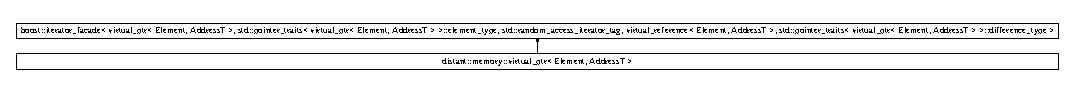
\includegraphics[height=0.704403cm]{classdistant_1_1memory_1_1virtual__ptr}
\end{center}
\end{figure}
\subsection*{Public Types}
\begin{DoxyCompactItemize}
\item 
\mbox{\Hypertarget{classdistant_1_1memory_1_1virtual__ptr_ac3e54c3aeee6754a34e24e4a197e7f28}\label{classdistant_1_1memory_1_1virtual__ptr_ac3e54c3aeee6754a34e24e4a197e7f28}} 
using {\bfseries element\+\_\+type} = typename std\+::pointer\+\_\+traits$<$ \mbox{\hyperlink{classdistant_1_1memory_1_1virtual__ptr}{virtual\+\_\+ptr}} $>$\+::element\+\_\+type
\item 
\mbox{\Hypertarget{classdistant_1_1memory_1_1virtual__ptr_a57c73631035f9adb29689dc8880f36fc}\label{classdistant_1_1memory_1_1virtual__ptr_a57c73631035f9adb29689dc8880f36fc}} 
using {\bfseries difference\+\_\+type} = typename std\+::pointer\+\_\+traits$<$ \mbox{\hyperlink{classdistant_1_1memory_1_1virtual__ptr}{virtual\+\_\+ptr}} $>$\+::difference\+\_\+type
\item 
\mbox{\Hypertarget{classdistant_1_1memory_1_1virtual__ptr_a8cf58b4f960ddffac40c0e9d7a7de0c6}\label{classdistant_1_1memory_1_1virtual__ptr_a8cf58b4f960ddffac40c0e9d7a7de0c6}} 
using {\bfseries reference} = \mbox{\hyperlink{classdistant_1_1memory_1_1virtual__reference}{virtual\+\_\+reference}}$<$ Element, AddressT $>$
\item 
\mbox{\Hypertarget{classdistant_1_1memory_1_1virtual__ptr_a5f6d081dc42a2a5ecb06eed60e16cb30}\label{classdistant_1_1memory_1_1virtual__ptr_a5f6d081dc42a2a5ecb06eed60e16cb30}} 
using {\bfseries const\+\_\+reference} = \mbox{\hyperlink{classdistant_1_1memory_1_1virtual__reference}{virtual\+\_\+reference}}$<$ const std\+::remove\+\_\+cv\+\_\+t$<$ Element $>$, AddressT $>$
\item 
\mbox{\Hypertarget{classdistant_1_1memory_1_1virtual__ptr_afb93921e8522362404fc705956c6a6ef}\label{classdistant_1_1memory_1_1virtual__ptr_afb93921e8522362404fc705956c6a6ef}} 
{\footnotesize template$<$typename T $>$ }\\using {\bfseries require\+\_\+vm\+\_\+access\+\_\+to} = std\+::enable\+\_\+if\+\_\+t$<$(\mbox{\hyperlink{structdistant_1_1memory_1_1detail_1_1required__vm__access}{detail\+::required\+\_\+vm\+\_\+access}}$<$ T $>$\+::value $>$=vm\+\_\+access) \&\&std\+::is\+\_\+convertible$<$ T, Element $>$\+::value, T $>$
\end{DoxyCompactItemize}
\subsection*{Public Member Functions}
\begin{DoxyCompactItemize}
\item 
\mbox{\Hypertarget{classdistant_1_1memory_1_1virtual__ptr_a41a69dbe4c826121b9a2105543baf894}\label{classdistant_1_1memory_1_1virtual__ptr_a41a69dbe4c826121b9a2105543baf894}} 
{\bfseries virtual\+\_\+ptr} (nullptr\+\_\+t) noexcept
\item 
\mbox{\Hypertarget{classdistant_1_1memory_1_1virtual__ptr_afab90fab354fb8126b466ba64d54059c}\label{classdistant_1_1memory_1_1virtual__ptr_afab90fab354fb8126b466ba64d54059c}} 
{\bfseries virtual\+\_\+ptr} (const \mbox{\hyperlink{classdistant_1_1kernel__objects_1_1process}{process}}$<$ vm\+\_\+access $>$ \&\mbox{\hyperlink{classdistant_1_1kernel__objects_1_1process}{process}}, \mbox{\hyperlink{classdistant_1_1memory_1_1address}{address}}$<$ AddressT $>$ \mbox{\hyperlink{classdistant_1_1memory_1_1address}{address}}=0) noexcept
\item 
\mbox{\Hypertarget{classdistant_1_1memory_1_1virtual__ptr_a825c03034067ef4f7355f039d5f8dc5c}\label{classdistant_1_1memory_1_1virtual__ptr_a825c03034067ef4f7355f039d5f8dc5c}} 
{\footnotesize template$<$typename OtherT , typename Other\+AddressT , typename  = require\+\_\+vm\+\_\+access\+\_\+to$<$\+Other\+T$>$$>$ }\\{\bfseries virtual\+\_\+ptr} (\mbox{\hyperlink{classdistant_1_1memory_1_1virtual__ptr}{virtual\+\_\+ptr}}$<$ OtherT, Other\+AddressT $>$ pointer) noexcept
\item 
\mbox{\Hypertarget{classdistant_1_1memory_1_1virtual__ptr_a531f1da61b77dbcb8ede230567692d0b}\label{classdistant_1_1memory_1_1virtual__ptr_a531f1da61b77dbcb8ede230567692d0b}} 
\mbox{\hyperlink{classdistant_1_1memory_1_1address}{address}}$<$ AddressT $>$ {\bfseries get} () const noexcept
\item 
\mbox{\Hypertarget{classdistant_1_1memory_1_1virtual__ptr_a9d3a380ad6f5068014769d55a414bc15}\label{classdistant_1_1memory_1_1virtual__ptr_a9d3a380ad6f5068014769d55a414bc15}} 
const \mbox{\hyperlink{classdistant_1_1kernel__objects_1_1process}{kernel\+\_\+objects\+::process}}$<$ vm\+\_\+access $>$ \& {\bfseries ambient\+\_\+process} () const noexcept
\end{DoxyCompactItemize}
\subsection*{Static Public Attributes}
\begin{DoxyCompactItemize}
\item 
\mbox{\Hypertarget{classdistant_1_1memory_1_1virtual__ptr_a1dacaef418accf1e994d51d25f734f65}\label{classdistant_1_1memory_1_1virtual__ptr_a1dacaef418accf1e994d51d25f734f65}} 
static constexpr auto {\bfseries vm\+\_\+access} = \mbox{\hyperlink{structdistant_1_1memory_1_1virtual__traits}{virtual\+\_\+traits}}$<$\mbox{\hyperlink{classdistant_1_1memory_1_1virtual__ptr}{virtual\+\_\+ptr}}$>$\+::vm\+\_\+access
\end{DoxyCompactItemize}
\subsection*{Friends}
\begin{DoxyCompactItemize}
\item 
\mbox{\Hypertarget{classdistant_1_1memory_1_1virtual__ptr_ac09f73e325921cc50ebcd96bed0f8096}\label{classdistant_1_1memory_1_1virtual__ptr_ac09f73e325921cc50ebcd96bed0f8096}} 
class {\bfseries boost\+::iterator\+\_\+core\+\_\+access}
\item 
\mbox{\Hypertarget{classdistant_1_1memory_1_1virtual__ptr_acebd62ead6c46eaab65bf9900edf2492}\label{classdistant_1_1memory_1_1virtual__ptr_acebd62ead6c46eaab65bf9900edf2492}} 
{\footnotesize template$<$typename E , typename T $>$ }\\class {\bfseries virtual\+\_\+reference}
\item 
\mbox{\Hypertarget{classdistant_1_1memory_1_1virtual__ptr_abd803c82999262af198dd4b0e0262801}\label{classdistant_1_1memory_1_1virtual__ptr_abd803c82999262af198dd4b0e0262801}} 
{\footnotesize template$<$typename E , typename T $>$ }\\class {\bfseries virtual\+\_\+ptr}
\end{DoxyCompactItemize}


The documentation for this class was generated from the following files\+:\begin{DoxyCompactItemize}
\item 
C\+:/\+Users/dinne/source/repos/distant dev/distant dev/include/distant/memory/fwd.\+hpp\item 
C\+:/\+Users/dinne/source/repos/distant dev/distant dev/include/distant/memory/virtual\+\_\+ptr.\+hpp\item 
C\+:/\+Users/dinne/source/repos/distant dev/distant dev/include/distant/memory/impl/virtual\+\_\+ptr.\+hxx\end{DoxyCompactItemize}

\hypertarget{classdistant_1_1memory_1_1virtual__reference}{}\section{distant\+:\+:memory\+:\+:virtual\+\_\+reference$<$ Element, AddressT $>$ Class Template Reference}
\label{classdistant_1_1memory_1_1virtual__reference}\index{distant\+::memory\+::virtual\+\_\+reference$<$ Element, Address\+T $>$@{distant\+::memory\+::virtual\+\_\+reference$<$ Element, Address\+T $>$}}
\subsection*{Public Types}
\begin{DoxyCompactItemize}
\item 
\mbox{\Hypertarget{classdistant_1_1memory_1_1virtual__reference_a090a34daa4d50c65e1f55da5b112c62b}\label{classdistant_1_1memory_1_1virtual__reference_a090a34daa4d50c65e1f55da5b112c62b}} 
using {\bfseries pointer} = typename std\+::pointer\+\_\+traits$<$ \mbox{\hyperlink{classdistant_1_1memory_1_1virtual__ptr}{virtual\+\_\+ptr}}$<$ Element, AddressT $>$ $>$\+::pointer
\item 
\mbox{\Hypertarget{classdistant_1_1memory_1_1virtual__reference_ad4e7bbf25b6c72240c08e08b11060c68}\label{classdistant_1_1memory_1_1virtual__reference_ad4e7bbf25b6c72240c08e08b11060c68}} 
using {\bfseries value\+\_\+type} = typename std\+::pointer\+\_\+traits$<$ \mbox{\hyperlink{classdistant_1_1memory_1_1virtual__ptr}{virtual\+\_\+ptr}}$<$ Element, AddressT $>$ $>$\+::element\+\_\+type
\item 
\mbox{\Hypertarget{classdistant_1_1memory_1_1virtual__reference_a43d4fc28c6ec679068ffd5163d6ee947}\label{classdistant_1_1memory_1_1virtual__reference_a43d4fc28c6ec679068ffd5163d6ee947}} 
{\footnotesize template$<$typename T $>$ }\\using {\bfseries require\+\_\+vm\+\_\+access\+\_\+to} = std\+::enable\+\_\+if\+\_\+t$<$ \mbox{\hyperlink{structdistant_1_1memory_1_1detail_1_1required__vm__access}{detail\+::required\+\_\+vm\+\_\+access}}$<$ T $>$\+::value $>$=vm\+\_\+access $>$
\end{DoxyCompactItemize}
\subsection*{Public Member Functions}
\begin{DoxyCompactItemize}
\item 
\mbox{\Hypertarget{classdistant_1_1memory_1_1virtual__reference_a14cb9b6c4f14334a9c98d38bd5187b7b}\label{classdistant_1_1memory_1_1virtual__reference_a14cb9b6c4f14334a9c98d38bd5187b7b}} 
{\bfseries virtual\+\_\+reference} (pointer ptr) noexcept
\item 
\mbox{\Hypertarget{classdistant_1_1memory_1_1virtual__reference_a5f3256bbfd67220c8e08b063deed43c8}\label{classdistant_1_1memory_1_1virtual__reference_a5f3256bbfd67220c8e08b063deed43c8}} 
{\footnotesize template$<$typename Other\+Element , typename Other\+AddressT , typename  = require\+\_\+vm\+\_\+access\+\_\+to$<$\+Other\+Element$>$$>$ }\\{\bfseries virtual\+\_\+reference} (\mbox{\hyperlink{classdistant_1_1memory_1_1virtual__reference}{virtual\+\_\+reference}}$<$ Other\+Element, Other\+AddressT $>$ other) noexcept
\item 
\mbox{\Hypertarget{classdistant_1_1memory_1_1virtual__reference_aa4cdb7a271a618acb61120702099b1d7}\label{classdistant_1_1memory_1_1virtual__reference_aa4cdb7a271a618acb61120702099b1d7}} 
{\footnotesize template$<$typename Other\+Element , typename Other\+AddressT , typename  = require\+\_\+vm\+\_\+access\+\_\+to$<$\+Other\+Element$>$$>$ }\\\mbox{\hyperlink{classdistant_1_1memory_1_1virtual__reference}{virtual\+\_\+reference}} \& {\bfseries operator=} (\mbox{\hyperlink{classdistant_1_1memory_1_1virtual__reference}{virtual\+\_\+reference}}$<$ Other\+Element, Other\+AddressT $>$ other) noexcept
\item 
\mbox{\Hypertarget{classdistant_1_1memory_1_1virtual__reference_a0b6a48d5de31a3b83a07b660d4c2127c}\label{classdistant_1_1memory_1_1virtual__reference_a0b6a48d5de31a3b83a07b660d4c2127c}} 
{\footnotesize template$<$typename Value , typename  = std\+::enable\+\_\+if\+\_\+t$<$					std\+::is\+\_\+convertible$<$\+Value, value\+\_\+type$>$\+::value \&\& 					!std\+::is\+\_\+const$<$\+Value$>$\+::value				$>$$>$ }\\\mbox{\hyperlink{classdistant_1_1memory_1_1virtual__reference}{virtual\+\_\+reference}} \& {\bfseries operator=} (const Value \&x)
\item 
\mbox{\Hypertarget{classdistant_1_1memory_1_1virtual__reference_a4862e98044e44bea303a7cb0f69837a1}\label{classdistant_1_1memory_1_1virtual__reference_a4862e98044e44bea303a7cb0f69837a1}} 
pointer {\bfseries operator \&} () const noexcept
\item 
\mbox{\Hypertarget{classdistant_1_1memory_1_1virtual__reference_aafca1ebac190375eb6a7c61a80c3a745}\label{classdistant_1_1memory_1_1virtual__reference_aafca1ebac190375eb6a7c61a80c3a745}} 
{\bfseries operator value\+\_\+type} () const
\item 
\mbox{\Hypertarget{classdistant_1_1memory_1_1virtual__reference_a4df2c5ec5426ade0787f65f5103e1975}\label{classdistant_1_1memory_1_1virtual__reference_a4df2c5ec5426ade0787f65f5103e1975}} 
void {\bfseries swap} (\mbox{\hyperlink{classdistant_1_1memory_1_1virtual__reference}{virtual\+\_\+reference}} \&other)
\item 
\mbox{\Hypertarget{classdistant_1_1memory_1_1virtual__reference_a198444ab95daf929c66c2b1852697f85}\label{classdistant_1_1memory_1_1virtual__reference_a198444ab95daf929c66c2b1852697f85}} 
\mbox{\hyperlink{classdistant_1_1memory_1_1virtual__reference}{virtual\+\_\+reference}} \& {\bfseries operator++} ()
\item 
\mbox{\Hypertarget{classdistant_1_1memory_1_1virtual__reference_abbe6e8da456b3078518b8cc0016e04c5}\label{classdistant_1_1memory_1_1virtual__reference_abbe6e8da456b3078518b8cc0016e04c5}} 
value\+\_\+type {\bfseries operator++} (int)
\item 
\mbox{\Hypertarget{classdistant_1_1memory_1_1virtual__reference_ac1efbb3eaecc44dcb172a84221827193}\label{classdistant_1_1memory_1_1virtual__reference_ac1efbb3eaecc44dcb172a84221827193}} 
\mbox{\hyperlink{classdistant_1_1memory_1_1virtual__reference}{virtual\+\_\+reference}} \& {\bfseries operator-\/-\/} ()
\item 
\mbox{\Hypertarget{classdistant_1_1memory_1_1virtual__reference_a59da90f9a5725fbba813238e0667b2f6}\label{classdistant_1_1memory_1_1virtual__reference_a59da90f9a5725fbba813238e0667b2f6}} 
value\+\_\+type {\bfseries operator-\/-\/} (int)
\item 
\mbox{\Hypertarget{classdistant_1_1memory_1_1virtual__reference_aa37c065bf2aebe45c6ab09ded283eb70}\label{classdistant_1_1memory_1_1virtual__reference_aa37c065bf2aebe45c6ab09ded283eb70}} 
\mbox{\hyperlink{classdistant_1_1memory_1_1virtual__reference}{virtual\+\_\+reference}} \& {\bfseries operator+=} (const value\+\_\+type \&rhs)
\item 
\mbox{\Hypertarget{classdistant_1_1memory_1_1virtual__reference_a9640b1d3df2eadd6e7ef28390f4367e2}\label{classdistant_1_1memory_1_1virtual__reference_a9640b1d3df2eadd6e7ef28390f4367e2}} 
\mbox{\hyperlink{classdistant_1_1memory_1_1virtual__reference}{virtual\+\_\+reference}} \& {\bfseries operator-\/=} (const value\+\_\+type \&rhs)
\item 
\mbox{\Hypertarget{classdistant_1_1memory_1_1virtual__reference_ae2d5551f38b87820182304e46d1cef28}\label{classdistant_1_1memory_1_1virtual__reference_ae2d5551f38b87820182304e46d1cef28}} 
\mbox{\hyperlink{classdistant_1_1memory_1_1virtual__reference}{virtual\+\_\+reference}} \& {\bfseries operator$\ast$=} (const value\+\_\+type \&rhs)
\item 
\mbox{\Hypertarget{classdistant_1_1memory_1_1virtual__reference_a10ae0aa83e390b28468d06f04321970e}\label{classdistant_1_1memory_1_1virtual__reference_a10ae0aa83e390b28468d06f04321970e}} 
\mbox{\hyperlink{classdistant_1_1memory_1_1virtual__reference}{virtual\+\_\+reference}} \& {\bfseries operator/=} (const value\+\_\+type \&rhs)
\item 
\mbox{\Hypertarget{classdistant_1_1memory_1_1virtual__reference_a0be66a6374d779acfad9c7905e8a413c}\label{classdistant_1_1memory_1_1virtual__reference_a0be66a6374d779acfad9c7905e8a413c}} 
\mbox{\hyperlink{classdistant_1_1memory_1_1virtual__reference}{virtual\+\_\+reference}} \& {\bfseries operator\%=} (const value\+\_\+type \&rhs)
\item 
\mbox{\Hypertarget{classdistant_1_1memory_1_1virtual__reference_a32b9224ec27044edb0e478621cdde667}\label{classdistant_1_1memory_1_1virtual__reference_a32b9224ec27044edb0e478621cdde667}} 
\mbox{\hyperlink{classdistant_1_1memory_1_1virtual__reference}{virtual\+\_\+reference}} \& {\bfseries operator$<$$<$=} (const value\+\_\+type \&rhs)
\item 
\mbox{\Hypertarget{classdistant_1_1memory_1_1virtual__reference_a20125d7872fa404b6df2488ce096362f}\label{classdistant_1_1memory_1_1virtual__reference_a20125d7872fa404b6df2488ce096362f}} 
\mbox{\hyperlink{classdistant_1_1memory_1_1virtual__reference}{virtual\+\_\+reference}} \& {\bfseries operator$>$$>$=} (const value\+\_\+type \&rhs)
\item 
\mbox{\Hypertarget{classdistant_1_1memory_1_1virtual__reference_ae6cf249bb2520a34a8ec43d54c1dbbe2}\label{classdistant_1_1memory_1_1virtual__reference_ae6cf249bb2520a34a8ec43d54c1dbbe2}} 
\mbox{\hyperlink{classdistant_1_1memory_1_1virtual__reference}{virtual\+\_\+reference}} \& {\bfseries operator \&=} (const value\+\_\+type \&rhs)
\item 
\mbox{\Hypertarget{classdistant_1_1memory_1_1virtual__reference_afc040b310fdbc8b8873681796542fd70}\label{classdistant_1_1memory_1_1virtual__reference_afc040b310fdbc8b8873681796542fd70}} 
\mbox{\hyperlink{classdistant_1_1memory_1_1virtual__reference}{virtual\+\_\+reference}} \& {\bfseries operator$\vert$=} (const value\+\_\+type \&rhs)
\item 
\mbox{\Hypertarget{classdistant_1_1memory_1_1virtual__reference_aaa76cb144af3d98d50cfcc826d31cbd5}\label{classdistant_1_1memory_1_1virtual__reference_aaa76cb144af3d98d50cfcc826d31cbd5}} 
\mbox{\hyperlink{classdistant_1_1memory_1_1virtual__reference}{virtual\+\_\+reference}} \& {\bfseries operator$^\wedge$=} (const value\+\_\+type \&rhs)
\item 
\mbox{\Hypertarget{classdistant_1_1memory_1_1virtual__reference_a6877c4d5d9728a2585507fc2a4cb2857}\label{classdistant_1_1memory_1_1virtual__reference_a6877c4d5d9728a2585507fc2a4cb2857}} 
{\footnotesize template$<$typename OE , typename OT , typename $>$ }\\{\bfseries virtual\+\_\+reference} (\mbox{\hyperlink{classdistant_1_1memory_1_1virtual__reference}{virtual\+\_\+reference}}$<$ OE, OT $>$ other) noexcept
\item 
\mbox{\Hypertarget{classdistant_1_1memory_1_1virtual__reference_a707f1268d986e8a94985fbc5a28a824c}\label{classdistant_1_1memory_1_1virtual__reference_a707f1268d986e8a94985fbc5a28a824c}} 
{\footnotesize template$<$typename OE , typename OT , typename $>$ }\\\mbox{\hyperlink{classdistant_1_1memory_1_1virtual__reference}{virtual\+\_\+reference}}$<$ E, T $>$ \& {\bfseries operator=} (\mbox{\hyperlink{classdistant_1_1memory_1_1virtual__reference}{virtual\+\_\+reference}}$<$ OE, OT $>$ other) noexcept
\item 
\mbox{\Hypertarget{classdistant_1_1memory_1_1virtual__reference_a89391719d337fe7387fa772a574ab402}\label{classdistant_1_1memory_1_1virtual__reference_a89391719d337fe7387fa772a574ab402}} 
{\footnotesize template$<$typename Value , typename $>$ }\\\mbox{\hyperlink{classdistant_1_1memory_1_1virtual__reference}{virtual\+\_\+reference}}$<$ E, T $>$ \& {\bfseries operator=} (const Value \&x)
\end{DoxyCompactItemize}
\subsection*{Static Public Attributes}
\begin{DoxyCompactItemize}
\item 
\mbox{\Hypertarget{classdistant_1_1memory_1_1virtual__reference_a35d50a515cc6b37dd7372b28ba6e163c}\label{classdistant_1_1memory_1_1virtual__reference_a35d50a515cc6b37dd7372b28ba6e163c}} 
static constexpr auto {\bfseries vm\+\_\+access} = \mbox{\hyperlink{structdistant_1_1memory_1_1virtual__traits}{virtual\+\_\+traits}}$<$\mbox{\hyperlink{classdistant_1_1memory_1_1virtual__reference}{virtual\+\_\+reference}}$>$\+::vm\+\_\+access
\end{DoxyCompactItemize}
\subsection*{Friends}
\begin{DoxyCompactItemize}
\item 
\mbox{\Hypertarget{classdistant_1_1memory_1_1virtual__reference_acebd62ead6c46eaab65bf9900edf2492}\label{classdistant_1_1memory_1_1virtual__reference_acebd62ead6c46eaab65bf9900edf2492}} 
{\footnotesize template$<$typename E , typename Ad $>$ }\\class {\bfseries virtual\+\_\+reference}
\item 
\mbox{\Hypertarget{classdistant_1_1memory_1_1virtual__reference_abd803c82999262af198dd4b0e0262801}\label{classdistant_1_1memory_1_1virtual__reference_abd803c82999262af198dd4b0e0262801}} 
{\footnotesize template$<$typename E , typename Ad $>$ }\\class {\bfseries virtual\+\_\+ptr}
\end{DoxyCompactItemize}


The documentation for this class was generated from the following files\+:\begin{DoxyCompactItemize}
\item 
C\+:/\+Users/dinne/source/repos/distant dev/distant dev/include/distant/memory/fwd.\+hpp\item 
C\+:/\+Users/dinne/source/repos/distant dev/distant dev/include/distant/memory/virtual\+\_\+reference.\+hpp\item 
C\+:/\+Users/dinne/source/repos/distant dev/distant dev/include/distant/memory/impl/virtual\+\_\+reference.\+hxx\end{DoxyCompactItemize}

\hypertarget{structdistant_1_1memory_1_1virtual__traits}{}\section{distant\+:\+:memory\+:\+:virtual\+\_\+traits$<$ Virtual $>$ Struct Template Reference}
\label{structdistant_1_1memory_1_1virtual__traits}\index{distant\+::memory\+::virtual\+\_\+traits$<$ Virtual $>$@{distant\+::memory\+::virtual\+\_\+traits$<$ Virtual $>$}}


The documentation for this struct was generated from the following file\+:\begin{DoxyCompactItemize}
\item 
C\+:/\+Users/dinne/source/repos/distant dev/distant dev/include/distant/memory/type\+\_\+traits.\+hpp\end{DoxyCompactItemize}

\hypertarget{structdistant_1_1memory_1_1virtual__traits_3_01virtual__ptr_3_01_element_00_01_address_t_01_4_01_4}{}\section{distant\+:\+:memory\+:\+:virtual\+\_\+traits$<$ virtual\+\_\+ptr$<$ Element, AddressT $>$ $>$ Struct Template Reference}
\label{structdistant_1_1memory_1_1virtual__traits_3_01virtual__ptr_3_01_element_00_01_address_t_01_4_01_4}\index{distant\+::memory\+::virtual\+\_\+traits$<$ virtual\+\_\+ptr$<$ Element, Address\+T $>$ $>$@{distant\+::memory\+::virtual\+\_\+traits$<$ virtual\+\_\+ptr$<$ Element, Address\+T $>$ $>$}}
Inheritance diagram for distant\+:\+:memory\+:\+:virtual\+\_\+traits$<$ virtual\+\_\+ptr$<$ Element, AddressT $>$ $>$\+:\begin{figure}[H]
\begin{center}
\leavevmode
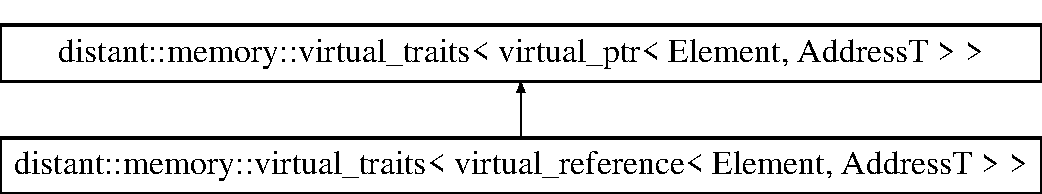
\includegraphics[height=2.000000cm]{structdistant_1_1memory_1_1virtual__traits_3_01virtual__ptr_3_01_element_00_01_address_t_01_4_01_4}
\end{center}
\end{figure}
\subsection*{Static Public Attributes}
\begin{DoxyCompactItemize}
\item 
\mbox{\Hypertarget{structdistant_1_1memory_1_1virtual__traits_3_01virtual__ptr_3_01_element_00_01_address_t_01_4_01_4_ac7737f243d20ae767ae91db79add8c1b}\label{structdistant_1_1memory_1_1virtual__traits_3_01virtual__ptr_3_01_element_00_01_address_t_01_4_01_4_ac7737f243d20ae767ae91db79add8c1b}} 
static constexpr auto {\bfseries vm\+\_\+access} = \mbox{\hyperlink{structdistant_1_1memory_1_1detail_1_1required__vm__access}{detail\+::required\+\_\+vm\+\_\+access}}$<$Element$>$\+::value
\end{DoxyCompactItemize}


The documentation for this struct was generated from the following file\+:\begin{DoxyCompactItemize}
\item 
C\+:/\+Users/dinne/source/repos/distant dev/distant dev/include/distant/memory/virtual\+\_\+ptr.\+hpp\end{DoxyCompactItemize}

\hypertarget{structdistant_1_1memory_1_1virtual__traits_3_01virtual__reference_3_01_element_00_01_address_t_01_4_01_4}{}\section{distant\+:\+:memory\+:\+:virtual\+\_\+traits$<$ virtual\+\_\+reference$<$ Element, AddressT $>$ $>$ Struct Template Reference}
\label{structdistant_1_1memory_1_1virtual__traits_3_01virtual__reference_3_01_element_00_01_address_t_01_4_01_4}\index{distant\+::memory\+::virtual\+\_\+traits$<$ virtual\+\_\+reference$<$ Element, Address\+T $>$ $>$@{distant\+::memory\+::virtual\+\_\+traits$<$ virtual\+\_\+reference$<$ Element, Address\+T $>$ $>$}}
Inheritance diagram for distant\+:\+:memory\+:\+:virtual\+\_\+traits$<$ virtual\+\_\+reference$<$ Element, AddressT $>$ $>$\+:\begin{figure}[H]
\begin{center}
\leavevmode
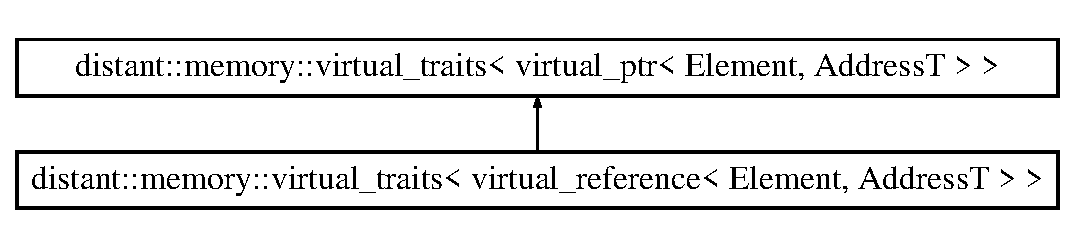
\includegraphics[height=2.000000cm]{structdistant_1_1memory_1_1virtual__traits_3_01virtual__reference_3_01_element_00_01_address_t_01_4_01_4}
\end{center}
\end{figure}
\subsection*{Additional Inherited Members}


The documentation for this struct was generated from the following file\+:\begin{DoxyCompactItemize}
\item 
C\+:/\+Users/dinne/source/repos/distant dev/distant dev/include/distant/memory/virtual\+\_\+reference.\+hpp\end{DoxyCompactItemize}

\hypertarget{classdistant_1_1synch_1_1wait}{}\section{distant\+:\+:synch\+:\+:wait Class Reference}
\label{classdistant_1_1synch_1_1wait}\index{distant\+::synch\+::wait@{distant\+::synch\+::wait}}
\subsection*{Classes}
\begin{DoxyCompactItemize}
\item 
class \mbox{\hyperlink{classdistant_1_1synch_1_1wait_1_1infinite}{infinite}}
\end{DoxyCompactItemize}
\subsection*{Public Types}
\begin{DoxyCompactItemize}
\item 
\mbox{\Hypertarget{classdistant_1_1synch_1_1wait_a32fac876e06a892057a902aeda135ea2}\label{classdistant_1_1synch_1_1wait_a32fac876e06a892057a902aeda135ea2}} 
enum {\bfseries state} \+: long long int \{ {\bfseries abandoned} = boost\+:\+:winapi\+:\+:W\+A\+I\+T\+\_\+\+A\+B\+A\+N\+D\+O\+N\+E\+D\+\_\+, 
{\bfseries signaled} = boost\+:\+:winapi\+:\+:W\+A\+I\+T\+\_\+\+O\+B\+J\+E\+C\+T\+\_\+0\+\_\+, 
{\bfseries timeout} = boost\+:\+:winapi\+:\+:W\+A\+I\+T\+\_\+\+T\+I\+M\+E\+O\+U\+T\+\_\+, 
{\bfseries failed} = boost\+:\+:winapi\+:\+:W\+A\+I\+T\+\_\+\+F\+A\+I\+L\+E\+D\+\_\+
 \}
\item 
\mbox{\Hypertarget{classdistant_1_1synch_1_1wait_ad3b91d21b04169ae77e5bc31ce1bc506}\label{classdistant_1_1synch_1_1wait_ad3b91d21b04169ae77e5bc31ce1bc506}} 
using {\bfseries time\+\_\+type} = boost\+::winapi\+::\+D\+W\+O\+R\+D\+\_\+
\end{DoxyCompactItemize}
\subsection*{Public Member Functions}
\begin{DoxyCompactItemize}
\item 
\mbox{\Hypertarget{classdistant_1_1synch_1_1wait_a090809d622ba2545bb2e61ea621efd5c}\label{classdistant_1_1synch_1_1wait_a090809d622ba2545bb2e61ea621efd5c}} 
{\footnotesize template$<$typename Kernel\+Object $>$ }\\wait\+::state {\bfseries operator()} (const Kernel\+Object \&obj, const time\+\_\+type time) const
\item 
\mbox{\Hypertarget{classdistant_1_1synch_1_1wait_a6e1e5bce76b3e4a5392a9392e0e8d369}\label{classdistant_1_1synch_1_1wait_a6e1e5bce76b3e4a5392a9392e0e8d369}} 
{\footnotesize template$<$typename Kernel\+Object $>$ }\\wait\+::state {\bfseries operator()} (const Kernel\+Object \&obj, \mbox{\hyperlink{classdistant_1_1synch_1_1wait_1_1infinite}{wait\+::infinite}} tag) const
\end{DoxyCompactItemize}


The documentation for this class was generated from the following file\+:\begin{DoxyCompactItemize}
\item 
C\+:/\+Users/dinne/source/repos/distant dev/distant dev/include/distant/synch/wait.\+hpp\end{DoxyCompactItemize}

\hypertarget{classdistant_1_1error_1_1windows__category}{}\section{distant\+:\+:error\+:\+:windows\+\_\+category Class Reference}
\label{classdistant_1_1error_1_1windows__category}\index{distant\+::error\+::windows\+\_\+category@{distant\+::error\+::windows\+\_\+category}}
Inheritance diagram for distant\+:\+:error\+:\+:windows\+\_\+category\+:\begin{figure}[H]
\begin{center}
\leavevmode
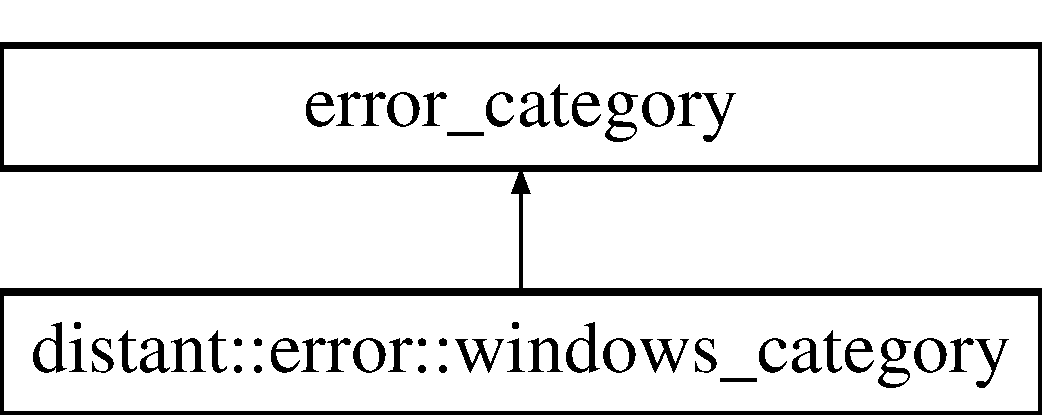
\includegraphics[height=2.000000cm]{classdistant_1_1error_1_1windows__category}
\end{center}
\end{figure}


The documentation for this class was generated from the following files\+:\begin{DoxyCompactItemize}
\item 
C\+:/\+Users/dinne/source/repos/distant dev/distant dev/include/distant/error/windows\+\_\+error.\+hpp\item 
C\+:/\+Users/dinne/source/repos/distant dev/distant dev/include/distant/error/impl/windows\+\_\+error.\+hxx\end{DoxyCompactItemize}

\hypertarget{classdistant_1_1error_1_1windows__error}{}\section{distant\+:\+:error\+:\+:windows\+\_\+error Class Reference}
\label{classdistant_1_1error_1_1windows__error}\index{distant\+::error\+::windows\+\_\+error@{distant\+::error\+::windows\+\_\+error}}
Inheritance diagram for distant\+:\+:error\+:\+:windows\+\_\+error\+:\begin{figure}[H]
\begin{center}
\leavevmode
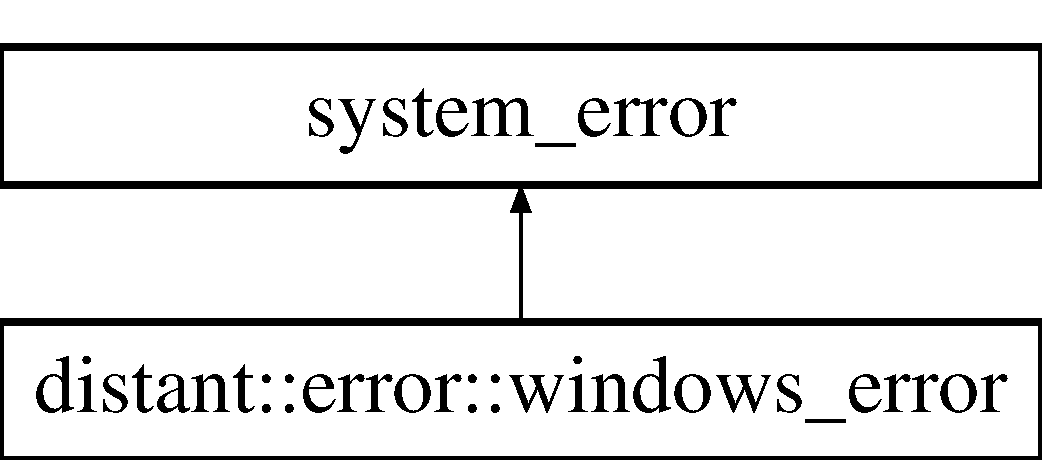
\includegraphics[height=2.000000cm]{classdistant_1_1error_1_1windows__error}
\end{center}
\end{figure}
\subsection*{Public Member Functions}
\begin{DoxyCompactItemize}
\item 
\mbox{\Hypertarget{classdistant_1_1error_1_1windows__error_a44323df6831761fbc7c820b5753d3a2d}\label{classdistant_1_1error_1_1windows__error_a44323df6831761fbc7c820b5753d3a2d}} 
{\bfseries windows\+\_\+error} (const std\+::string \&message)
\end{DoxyCompactItemize}


The documentation for this class was generated from the following files\+:\begin{DoxyCompactItemize}
\item 
C\+:/\+Users/dinne/source/repos/distant dev/distant dev/include/distant/error/windows\+\_\+error.\+hpp\item 
C\+:/\+Users/dinne/source/repos/distant dev/distant dev/include/distant/error/impl/windows\+\_\+error.\+hxx\end{DoxyCompactItemize}

\hypertarget{classdistant_1_1error_1_1windows__error__code}{}\section{distant\+:\+:error\+:\+:windows\+\_\+error\+\_\+code Class Reference}
\label{classdistant_1_1error_1_1windows__error__code}\index{distant\+::error\+::windows\+\_\+error\+\_\+code@{distant\+::error\+::windows\+\_\+error\+\_\+code}}


Windows error code.  




{\ttfamily \#include $<$windows\+\_\+error.\+hpp$>$}

Inheritance diagram for distant\+:\+:error\+:\+:windows\+\_\+error\+\_\+code\+:\begin{figure}[H]
\begin{center}
\leavevmode
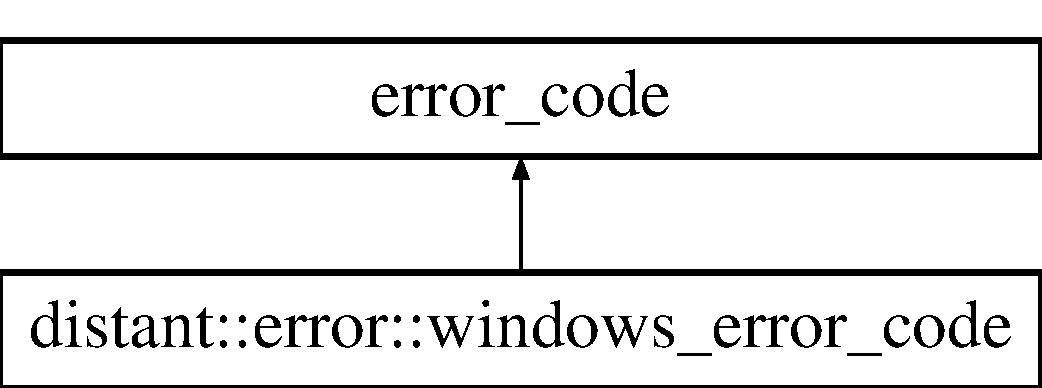
\includegraphics[height=2.000000cm]{classdistant_1_1error_1_1windows__error__code}
\end{center}
\end{figure}
\subsection*{Public Member Functions}
\begin{DoxyCompactItemize}
\item 
\mbox{\Hypertarget{classdistant_1_1error_1_1windows__error__code_a79178309b742d651f897310cb42c4ffc}\label{classdistant_1_1error_1_1windows__error__code_a79178309b742d651f897310cb42c4ffc}} 
\mbox{\hyperlink{classdistant_1_1error_1_1windows__error__code_a79178309b742d651f897310cb42c4ffc}{windows\+\_\+error\+\_\+code}} (boost\+::winapi\+::\+D\+W\+O\+R\+D\+\_\+ code) noexcept
\begin{DoxyCompactList}\small\item\em Construct an error code with the given code. \end{DoxyCompactList}\item 
\mbox{\Hypertarget{classdistant_1_1error_1_1windows__error__code_a2161718f19065dd703e9dce8a43a02e9}\label{classdistant_1_1error_1_1windows__error__code_a2161718f19065dd703e9dce8a43a02e9}} 
\mbox{\hyperlink{classdistant_1_1error_1_1windows__error__code_a2161718f19065dd703e9dce8a43a02e9}{windows\+\_\+error\+\_\+code}} (\mbox{\hyperlink{structdistant_1_1error_1_1gle}{gle}}) noexcept
\begin{DoxyCompactList}\small\item\em Construct an error code with the code obtained from \+::\+Get\+Last\+Error. \end{DoxyCompactList}\item 
\mbox{\Hypertarget{classdistant_1_1error_1_1windows__error__code_af7c2a999f121500dfd5be60a2d3e62ee}\label{classdistant_1_1error_1_1windows__error__code_af7c2a999f121500dfd5be60a2d3e62ee}} 
\mbox{\hyperlink{classdistant_1_1error_1_1windows__error__code_af7c2a999f121500dfd5be60a2d3e62ee}{windows\+\_\+error\+\_\+code}} () noexcept
\begin{DoxyCompactList}\small\item\em Construct an error code with no error. \end{DoxyCompactList}\item 
\mbox{\Hypertarget{classdistant_1_1error_1_1windows__error__code_a39a117bda3aed58ff21b5dff64488314}\label{classdistant_1_1error_1_1windows__error__code_a39a117bda3aed58ff21b5dff64488314}} 
void \mbox{\hyperlink{classdistant_1_1error_1_1windows__error__code_a39a117bda3aed58ff21b5dff64488314}{update\+\_\+last}} () noexcept
\begin{DoxyCompactList}\small\item\em Update the error code. \end{DoxyCompactList}\item 
\mbox{\Hypertarget{classdistant_1_1error_1_1windows__error__code_ac67c1fc88b2acdfd61d36d424c513de4}\label{classdistant_1_1error_1_1windows__error__code_ac67c1fc88b2acdfd61d36d424c513de4}} 
void {\bfseries set\+\_\+success} () noexcept
\item 
\mbox{\Hypertarget{classdistant_1_1error_1_1windows__error__code_a6a6337d6d1605ebc983330c8e3874747}\label{classdistant_1_1error_1_1windows__error__code_a6a6337d6d1605ebc983330c8e3874747}} 
void {\bfseries set} (boost\+::winapi\+::\+D\+W\+O\+R\+D\+\_\+ code) noexcept
\end{DoxyCompactItemize}


\subsection{Detailed Description}
Windows error code. 

The documentation for this class was generated from the following files\+:\begin{DoxyCompactItemize}
\item 
C\+:/\+Users/dinne/source/repos/distant dev/distant dev/include/distant/error/windows\+\_\+error.\+hpp\item 
C\+:/\+Users/dinne/source/repos/distant dev/distant dev/include/distant/error/impl/windows\+\_\+error.\+hxx\end{DoxyCompactItemize}

%--- End generated contents ---

% Index
\backmatter
\newpage
\phantomsection
\clearemptydoublepage
\addcontentsline{toc}{chapter}{Index}
\printindex

\end{document}
